\chapter{Anwendungsbeispiel auf simulierte Daten}
\label{chap:4}

In diesem Kapitel untersuchen wir die Leistung unseres Neuronale-Netze"=Regressionsschätzers aus Kapitel~\ref{chap:2} anhand von Anwendungsbeispielen auf simulierte Daten. Der Schätzer und die Beispiele wurden in \emph{Python}~\cite[Version 3.7.3]{van1995python} implementiert (vgl.\@ Appendix~\ref{chap:app}). 
%Dafür führen wir eine Simulation bei endlicher Stichprobengröße auf simulierte Daten durch.
Im ersten Abschnitt führen wir eine Parameterstudie für unseren Neuronale-Netze-Regressionsschätzer durch. Im zweiten Abschnitt quantifizieren wir im Rahmen eines Simulationsbeispiels die Leistung unseres Neuronale-Netze-Regressionsschätzers, indem wir den empirischen $L_2$-Fehler dieses Schätzers und weiterer Standardschätzer berechnen und vergleichen.
%Die Implementation der Standardschätzer erfolgte mithilfe der $Keras$ Bibliothek \cite{chollet2015keras}. Keras ist eine \emph{High-Level} Anwendungs-Programmierschnittstelle für neuronale Netze in Python. Wir haben uns für Keras entschieden, da diese Bibliothek einfaches und schnelles Erstellen von neuronalen Netzen durch Benutzerfreundlichkeit, Modularität und Erweiterbarkeit ermöglicht. 

\section{Parameterstudie}
\label{Studie}

In diesem Abschnitt führen wir für unseren Neuronale-Netze-Regressionsschätzer \textit{new\_neural\_network\_estimate} ($m_{n,1}$) eine Parameterstudie durch, um den Einfluss der Parameter auf den Schätzer zu überprüfen. Wir haben als Regressionsfunktion $m\colon [-3,3] \to \R$ mit
$$m(x) = \sin\big(\frac{\pi}{2} \cdot x^2\big)$$
gewählt.
Diese Funktion stellt als Potenzreihe und durch ihr starkes Schwingen für Regressionsschätzer und insbesondere für unseren Neuronale-Netze-Schätzer, welcher Polynome approximiert, eine Herausforderung dar. Wir erzeugen eine Stichprobe von $1000$ unabhängigen auf dem Intervall $[-3,3]$ gleichverteilten Zufallsvariablen und teilen diese Stichprobe in ein Learning-Sample der Größe $800$ und ein Testing-Sample \todo{was mach ich mit dem Sample? dieses Y aus Teil 2 brauch ich auch schon ...} der Größe $200$ auf. In der Parameterstudie verändern wir bei unserem Neuronale-Netze-Schätzer den Parameter~$N$, welcher den maximalen Grad der Polynome bestimmt, welche wir mit $f_{\net,\bj,\bi}$ schätzen möchten und die ihrerseits die Regressionsfunktion approximieren sollen (vgl.\@ Lemma~\ref{lem:5}). Zudem verändern wir den Parameter~$M$, welcher den Abstand zwischen zwei benachbarten Gitterpunkten steuert. Durch wachsendes $M$ verfeinert sich das Gitter, welches wir über das Intervall $[-3,3]$ legen und wir vermuten, dass sich dadurch die Approximationsgüte verbessert (vgl.\@ Lemma~\ref{lem:pcsmooth}). 

Um die Vergleichbarkeit der Ergebnisse sicherzustellen, erzeugen wir mit einem \emph{Seed} eine reproduzierbare Realisierung der Zufallsvariablen. In der Parameterstudie betrachten wir den Neuronale-Netze-Regressionsschätzer mit Parametern $d = 1$, $q = 2$, $R = 10^6$, $a = 3$, $M \in\{2,4,8,9,16\}$ und $N \in \{2,4,8,9,16\}$. Für die Wahl der Parameter haben wir uns an \cite{kohler19} orientiert.

In Abbildung~\ref{fig:subfig.a.1} erkennen wir die Approximation der Regressionsfunktion $m$ auf dem Testing-Sample durch unseren Neuronale-Netze-Regressionsschätzer, wobei wir $M = 2$ und $N \in \{2,4,8,16\}$ wählen. Visuell erkennen wir, dass sich die Approximation mit steigendem $N$ verbessert.
In Abbildung~\ref{fig:subfig.a.2} erkennen wir die Approximation der Regressionsfunktion $m$ auf dem Testing-Sample durch unseren Neuronale-Netze-Regressionsschätzer, wobei wir $N = 2$ und $M \in \{2,4,8,16\}$ wählen. Visuell erkennen wir, dass sich die Approximation mit steigendem $M$ verbessert. In Abbildung~\ref{fig:subfig.a.3} haben wir $N = 16$ fest gewählt und betrachten variables $M \in \{2,4,8,16\}$. Visuell erkennen wir, dass sich die Approximation mit steigendem $M$ verbessert.
In Abbildung~\ref{fig:subfig.a.4} haben wir $M = 16$ fest gewählt und betrachten variables $N \in \{2,4,8,16\}$. Visuell erkennen wir, dass sich die Approximation mit steigendem $N$ verbessert.
In Abbildung~\ref{fig:subfig.a.5} betrachten wir $M \in \{2,4,8,9,16\}$ und $N \in \{2,4,8,9,16\}$, wobei wir immer Kombinationen von $M$ und $N$ betrachten, sodass $(M + 1)\cdot(N + 1) \approx 51$ ergibt. Visuell erkennen wir, dass die Approximation besser ist, wenn einer der Parameter sehr groß ist, als wenn der kleiner Wert etwas höher und dafür der höhere etwas kleiner wird. Es ist zu beachten, dass die Approximation durch den Schätzer besser wird je höher die Parameter sind. Hohe Parameter führen aber auch zu einem höheren Ressourcenbedarf wie z.B. der Rechenzeit. Es ist daher auch interessant zu wissen, ob der Schätzer auch bei geringer Parameterwahl akzeptable Ergebnisse liefert. \todo{Sinn von Test und Sätze anders aufschreiben}
\begin{figure}
    \begin{subfigure}[b]{0.5\textwidth}
        \centering
        \scalebox{0.9}{
          % This file was created by tikzplotlib v0.9.0.
\begin{tikzpicture}

\begin{axis}[
tick align=outside,
tick pos=left,
title={$N = 2$, $M = 2$},
x grid style={white!69.0196078431373!black},
xmin=-3.34207441715318, xmax=3.35388433148518,
xtick style={color=black},
y grid style={white!69.0196078431373!black},
ymin=\ymin, ymax=\ymax,
ytick style={color=black}
]
\addplot [only marks, mark=x, draw=red, fill=red, colormap/viridis]
table{%
x                      y
2.76238288932011 0.0696236318238279
-2.97867143721344 0.633737080000907
1.34016626636584 0.248714554967007
-2.34602979642214 -0.182357969914886
0.262724949982951 0.276579929762546
0.761496100082008 0.579943587033136
-1.54231724537519 0.137487826890353
2.48306325147965 -0.209050168109025
0.733875172149707 0.581862620438073
-1.60983185163084 0.0944463650714438
1.62079312559885 0.0128238998441449
-2.36695752001599 -0.169806042172586
0.331351911188067 0.366935291492553
-2.43026358118505 -0.148779202921674
0.485904436050117 0.50608690784783
-1.48211932367887 0.182067639405539
0.896800847728478 0.540051784810156
1.29496171714908 0.303477121481799
0.145113687411967 0.0773410376422204
0.945128446218661 0.524945754879947
1.87976307195033 -0.191036365260491
1.84507362985819 -0.133432065216717
0.718091952323177 0.570885589137396
-0.293385227275351 0.310656856937984
-0.552300065715795 0.51805352131015
2.24848571942618 -0.281705380200185
1.21759039268623 0.345041357964498
-1.89038986575959 -0.110954426485695
0.39439287977558 0.42502169868815
2.45284819380034 -0.291049415195146
-2.09586004651037 -0.174790102547986
2.07310605318424 -0.258593913584902
1.9212147978921 -0.20819892091787
-0.00395339221299285 -0.213846884924733
-2.77449689108578 0.221864318492094
-2.11498496761839 -0.189604387705741
2.53583216813203 -0.186964112299095
-2.73507122380883 0.152535754337504
-0.765007401567843 0.567667271209152
0.714237808352825 0.574790029524826
-1.8183117665159 -0.0678797541792888
2.88647854344178 0.328580875841696
-2.06414860173947 -0.197580498970857
0.238075170967647 0.234706842829697
0.708067946079868 0.563210486112765
-1.61406030798178 0.0824455711739863
-0.202146064743951 0.181958653527321
-0.0539488252024247 -0.106001454253169
1.60117425795925 0.0268839866227892
0.80568451664324 0.569994864268828
-0.194699681607962 0.155109836510655
1.00165525916385 0.493954542768638
-0.27973544086681 0.289157685130155
0.154269548048458 0.0956456982377724
0.951408249350171 0.520713845991454
-1.91282770827683 -0.127397947271127
1.72829730703384 -0.0981881929027961
0.617192025230384 0.55205086222802
2.88199731082397 0.257672602530644
-1.66570083881295 0.0289289295878304
-0.202401155000559 0.173928900889795
2.37385081559668 -0.282189394553184
0.608600458192729 0.551859514930808
1.35575307509289 0.240605729820491
-0.517979014791838 0.509784695143142
1.10585773098792 0.433697362702257
2.67633017908538 -0.0581264373606373
-1.79888360556407 -0.0548319027405837
1.84419158326392 -0.16453292485422
2.81722807259938 0.129299858654392
-2.91258760942001 0.462533316200221
-1.70874248043343 -0.00265669709421586
-2.29573847812122 -0.197860934334551
1.60454110644872 0.0123043503044086
-2.5127004843436 -0.100211621541327
2.99048135154545 0.580477883172723
-0.662327904724169 0.562940735546021
2.43121659559824 -0.261737470590812
-1.86853437900319 -0.0867912316975652
-0.354766801066255 0.377849280746422
2.06887091403722 -0.263172932170869
0.571618684039537 0.540758268586486
-0.227051419851858 0.208952653519809
0.0758984805427056 -0.0660598577993334
0.443313161354085 0.467849231283596
-0.358084754486441 0.381040306623068
-1.83864625365714 -0.0820334262989837
-2.31620543124488 -0.185655582899956
-2.09263243577911 -0.193333018106388
-2.6850542168812 0.0741495862569121
0.352058466381789 0.400423386956392
2.08632608421606 -0.282303520605454
-0.845283966455336 0.561303048771281
-2.54813476418509 -0.0782902428983408
-0.445653528089303 0.462311761039538
0.612047030832008 0.551986963974434
-0.447579206546175 0.459834061505772
1.86432740164422 -0.179658424288866
2.65131747712023 -0.0627350597311313
2.21946463961013 -0.307059454464259
1.22399698967933 0.345021100869182
-0.178206451306949 0.1319605260999
1.09618825741951 0.429667535760761
-2.91949013666082 0.488183705540907
2.89486871101226 0.352203562036919
-1.96753600902662 -0.16045119359885
2.43756237577009 -0.288929628562372
1.84265940999664 -0.161298104879786
1.80083810632193 -0.141055692020237
-1.38638365328961 0.251869349071475
-1.68507716545645 0.0246260328122515
-0.427195842515467 0.443204831149814
2.09622660438393 -0.296207948253234
-0.297722145169678 0.312538376398336
2.61252068404237 -0.134573678836577
-0.883924036489572 0.546033270670057
0.716352994180558 0.570243797957124
2.88419421813468 0.263470255215231
0.86077513344483 0.544442885926027
-2.72701070375638 0.125755209385306
-0.218657454289729 0.195394301722511
-0.991491937718017 0.505110821563645
0.193089291130048 0.171200551825321
-1.29152274832121 0.329947721561154
-2.26643261861998 -0.190159426463652
1.00973393250481 0.502298921982884
1.08815852934784 0.455020376152709
2.20283579999453 -0.285933767539575
-2.20571103862358 -0.201050492351098
1.79172184966819 -0.111927190509838
1.96061243043077 -0.219791303528054
0.879299614506912 0.545472812107093
-1.7704671253162 -0.0291843733066064
-1.43147571356497 0.227746932556877
-0.489019094764946 0.487883854119478
0.250794436696388 0.274569478277348
-0.135372266446698 0.0500974715983145
-0.195240647727783 0.162354897047872
2.039044261186 -0.292797146638685
2.22061419184541 -0.287449503098603
1.9005237862606 -0.192106090073864
2.2668085118082 -0.274119117160396
0.426052571622439 0.44960618800233
2.78421680003449 0.140845652944863
0.639266089502806 0.572103220112891
0.623686446478088 0.553399251051943
-1.08421357755229 0.460697208765001
1.08722510470211 0.450440988578061
-2.68820586896783 0.0913492374542259
-2.19272147392835 -0.199964350161324
-2.21854699456341 -0.202163173332134
0.931207723348414 0.52067877587295
-1.94800444937197 -0.153516583129393
-0.953119060490716 0.52563240549111
-2.73413006500137 0.165634437169029
-1.59759383930094 0.086424839086587
2.78534594909577 0.142258860244893
0.0548364150982064 -0.0927990326237934
-2.09355288917141 -0.193557648022957
0.138051190406785 0.0789920873749814
2.66105630346648 -0.0658396521506408
2.194116084038 -0.295449086285518
-0.647604786417679 0.564919032371968
-1.29679490415958 0.313336184944381
1.57037917615645 0.0221899214320187
-1.55709405118147 0.121053137557245
-1.47460587205589 0.180047593251032
-2.49548187492042 -0.117716440387838
2.18486456858416 -0.330379017657128
-0.312606506278321 0.34142705463999
0.370717563659841 0.409033019659376
1.42026574616112 0.160195775442276
1.77893320278717 -0.109328186028923
-0.314951166058117 0.333188366110346
-1.89523466294521 -0.111587123211569
1.97239710916981 -0.220964999610406
-2.81401224103046 0.273043906979287
2.68036961764771 -0.0263855368729497
0.461867078865009 0.487366450058124
2.25233243070412 -0.302674491559908
0.651392621841352 0.565401484012899
-1.49004249508606 0.187522044760347
-1.22322045902457 0.368519554333596
0.197535354189919 0.18369781959133
2.77246927708256 0.0889320961106456
-1.89302637305893 -0.112964568570176
0.0593902688586541 -0.082299678630407
-0.937271379378934 0.530946198776765
1.61835206974311 0.0172177591909828
1.81719891859454 -0.147646715163199
-0.4526405381867 0.455338576591202
-1.77526500003398 -0.0287151264295879
-2.59746323802687 -0.0327566121202083
-1.80811041347663 -0.0564382347081382
-1.36559489922371 0.274966941442125
0.592733507455263 0.5512862734667
2.23850098364661 -0.301633261716772
-2.23061436692708 -0.202017047050301
2.74913245028938 -0.0145682835209204
1.09902506312488 0.438680147808397
};
\addplot [semithick, black]
table {%
-3 1
-2.99 0.995576734820054
-2.98 0.982404791977482
-2.97 0.960687140310815
-2.96 0.930698746339696
-2.95 0.892782465918225
-2.94 0.847344438774256
-2.93 0.794849046139829
-2.92 0.735813493407208
-2.91 0.670802080787205
-2.9 0.6004202253259
-2.89 0.525308297382294
-2.88 0.446135333817727
-2.87 0.363592688736647
-2.86 0.278387680690676
-2.85 0.191237292858769
-2.84 0.102861979893671
-2.83 0.0139796319282911
-2.82 -0.0747002572851044
-2.81 -0.162482174923344
-2.8 -0.248689887164819
-2.79 -0.332671415810564
-2.78 -0.413803662790115
-2.77 -0.491496656276015
-2.76000000000001 -0.565197396549224
-2.75000000000001 -0.63439328416361
-2.74000000000001 -0.698615117310616
-2.73000000000001 -0.7574396495474
-2.72000000000001 -0.810491703188593
-2.71000000000001 -0.857445837641644
-2.70000000000001 -0.898027575760592
-2.69000000000001 -0.932014194877928
-2.68000000000001 -0.959235092527838
-2.67000000000001 -0.979571739978357
-2.66000000000001 -0.992957239530362
-2.65000000000001 -0.999375504106505
-2.64000000000001 -0.998860079935072
-2.63000000000001 -0.991492635127341
-2.62000000000001 -0.977401138650261
-2.61000000000001 -0.956757755609883
-2.60000000000001 -0.929776485888277
-2.59000000000001 -0.896710574023413
-2.58000000000001 -0.857849718795458
-2.57000000000001 -0.813517111294285
-2.56000000000001 -0.764066330303094
-2.55000000000001 -0.709878123655345
-2.54000000000001 -0.651357103821107
-2.53000000000001 -0.588928385370132
-2.52000000000001 -0.523034191158988
-2.51000000000001 -0.454130453115695
-2.50000000000001 -0.382683432365167
-2.49000000000001 -0.309166382170306
-2.48000000000001 -0.234056275775223
-2.47000000000001 -0.157830619746354
-2.46000000000001 -0.0809643718325892
-2.45000000000001 -0.00392698072389465
-2.44000000000001 0.072820436603254
-2.43000000000001 0.148827765990005
-2.42000000000001 0.223658403427451
-2.41000000000001 0.296891588141009
-2.40000000000001 0.368124552684589
-2.39000000000001 0.43697448301218
-2.38000000000001 0.503080283168017
-2.37000000000001 0.56610414086275
-2.36000000000001 0.625732891772279
-2.35000000000001 0.681679181898872
-2.34000000000001 0.733682428763456
-2.33000000000001 0.781509583546624
-2.32000000000001 0.824955697558263
-2.31000000000001 0.863844297587357
-2.30000000000001 0.898027575760569
-2.29000000000002 0.927386400518292
-2.28000000000002 0.951830156198068
-2.27000000000002 0.971296419496836
-2.26000000000002 0.985750481765479
-2.25000000000002 0.995184726672186
-2.24000000000002 0.999617873256875
-2.23000000000002 0.999094094789406
-2.22000000000002 0.993682024142277
-2.21000000000002 0.983473656597255
-2.20000000000002 0.96858316112866
-2.19000000000002 0.949145611247931
-2.18000000000002 0.925315646459183
-2.17000000000002 0.897266075268519
-2.16000000000002 0.865186430515806
-2.15000000000002 0.829281487561826
-2.14000000000002 0.789769755571343
-2.13000000000002 0.746881951789148
-2.12000000000002 0.700859468316991
-2.11000000000002 0.651952840469899
-2.10000000000002 0.600420225325985
-2.09000000000002 0.546525898589853
-2.08000000000002 0.490538777371198
-2.07000000000002 0.432730975942088
-2.06000000000002 0.373376400983612
-2.05000000000002 0.31274939226965
-2.04000000000002 0.251123414166708
-2.03000000000002 0.188769802758421
-2.02000000000002 0.125956572835066
-2.01000000000002 0.062947288426061
-2.00000000000002 1.33870012014889e-13
-1.99000000000002 -0.062633749083271
-1.98000000000002 -0.124709844813965
-1.97000000000002 -0.185992451913749
-1.96000000000002 -0.246254789302508
-1.95000000000002 -0.305279831055913
-1.94000000000002 -0.3628609327075
-1.93000000000002 -0.418802383167873
-1.92000000000002 -0.472919882928091
-1.91000000000002 -0.525040949582032
-1.90000000000002 -0.575005252043164
-1.89000000000002 -0.622664875144035
-1.88000000000002 -0.667884516592001
-1.87000000000002 -0.710541618511978
-1.86000000000002 -0.750526436036607
-1.85000000000002 -0.787742045606543
-1.84000000000002 -0.822104295818981
-1.83000000000002 -0.85354170381174
-1.82000000000003 -0.881995300293982
-1.81000000000003 -0.907418426433774
-1.80000000000003 -0.929776485888198
-1.79000000000003 -0.949046655314642
-1.78000000000003 -0.965217556733346
-1.77000000000003 -0.978288895122437
-1.76000000000003 -0.988271064618766
-1.75000000000003 -0.995184726672183
-1.74000000000003 -0.99906036345861
-1.73000000000003 -0.999937809799883
-1.72000000000003 -0.997865766766904
-1.71000000000003 -0.992901300058717
-1.70000000000003 -0.985109326154799
-1.69000000000003 -0.974562089132473
-1.68000000000003 -0.961338630927184
-1.67000000000003 -0.945524257691589
-1.66000000000003 -0.92721000478115
-1.65000000000003 -0.906492102760418
-1.64000000000003 -0.883471446686396
-1.63000000000003 -0.858253070784441
-1.62000000000003 -0.830945630488965
-1.61000000000003 -0.801660893676759
-1.60000000000003 -0.770513242775885
-1.59000000000003 -0.737619189288572
-1.58000000000003 -0.703096902123257
-1.57000000000003 -0.667065750989361
-1.56000000000003 -0.629645865969377
-1.55000000000003 -0.590957714246878
-1.54000000000003 -0.5511216948366
-1.53000000000003 -0.510257752034371
-1.52000000000003 -0.468485008180726
-1.51000000000003 -0.425921416212823
-1.50000000000003 -0.382683432365229
-1.49000000000003 -0.338885709271396
-1.48000000000003 -0.29464080961443
-1.47000000000003 -0.250058940378286
-1.46000000000003 -0.205247707658841
-1.45000000000003 -0.16031189190854
-1.44000000000003 -0.115353243408457
-1.43000000000003 -0.0704702976877775
-1.42000000000003 -0.0257582105426693
-1.41000000000003 0.018691387755514
-1.40000000000003 0.0627905195291638
-1.39000000000003 0.106454968557562
-1.38000000000003 0.149604371296494
-1.37000000000003 0.192162291056312
-1.36000000000003 0.234056275774993
-1.35000000000004 0.275217900052248
-1.34000000000004 0.315582792135412
-1.33000000000004 0.355090646567928
-1.32000000000004 0.393685223226887
-1.31000000000004 0.431314333487567
-1.30000000000004 0.467929814260443
-1.29000000000004 0.503487490649953
-1.28000000000004 0.537947127984647
-1.27000000000004 0.571272373965398
-1.26000000000004 0.603430691672474
-1.25000000000004 0.634393284163532
-1.24000000000004 0.664135011383361
-1.23000000000004 0.692634300092632
-1.22000000000004 0.719873047507249
-1.21000000000004 0.745836519322339
-1.20000000000004 0.770513242775697
-1.19000000000004 0.79389489538482
-1.18000000000004 0.815976189969678
-1.17000000000004 0.836754756550324
-1.16000000000004 0.856231021684473
-1.15000000000004 0.87440808578545
-1.14000000000004 0.891291598935659
-1.13000000000004 0.906889635684947
-1.12000000000004 0.921212569297285
-1.11000000000004 0.93427294588298
-1.10000000000004 0.9460853588275
-1.09000000000004 0.956666323901834
-1.08000000000004 0.966034155413461
-1.07000000000004 0.974208843731348
-1.06000000000004 0.981211934493193
-1.05000000000004 0.987066409778344
-1.04000000000004 0.991796571505593
-1.03000000000004 0.995427927291427
-1.02000000000004 0.997987078981312
-1.01000000000004 0.999501614044331
-1.00000000000004 1
-0.990000000000043 0.999511482025296
-0.980000000000043 0.998065983870084
-0.970000000000043 0.995694012190007
-0.960000000000043 0.992426564387702
-0.950000000000044 0.988295040035889
-0.940000000000044 0.983331155939389
-0.930000000000044 0.977566864877576
-0.920000000000044 0.971034278054095
-0.910000000000045 0.963765591266851
-0.900000000000045 0.955793014798367
-0.890000000000045 0.94714870701456
-0.880000000000045 0.937864711648732
-0.870000000000045 0.927972898737259
-0.860000000000046 0.917504909163832
-0.850000000000046 0.906492102760406
-0.840000000000046 0.894965509904969
-0.830000000000046 0.882955786549018
-0.820000000000046 0.870493172601118
-0.810000000000047 0.857607453587072
-0.800000000000047 0.844327925502078
-0.790000000000047 0.830683362765738
-0.780000000000047 0.816701989186866
-0.770000000000048 0.802411451841723
-0.760000000000048 0.787838797766522
-0.750000000000048 0.773010453362809
-0.740000000000048 0.757952206412552
-0.730000000000048 0.742689190598499
-0.720000000000049 0.727245872424471
-0.710000000000049 0.711646040429847
-0.700000000000049 0.695912796592392
-0.690000000000049 0.68006854981388
-0.680000000000049 0.664135011383549
-0.67000000000005 0.648133192315342
-0.66000000000005 0.632083402456062
-0.65000000000005 0.61600525126299
-0.64000000000005 0.599917650151169
-0.630000000000051 0.583838816312412
-0.620000000000051 0.567786277910133
-0.610000000000051 0.551776880556293
-0.600000000000051 0.535826794979078
-0.590000000000051 0.519951525792427
-0.580000000000052 0.504165921281037
-0.570000000000052 0.488484184117171
-0.560000000000052 0.472919882928293
-0.550000000000052 0.457485964637341
-0.540000000000052 0.442194767500267
-0.530000000000053 0.427058034768333
-0.520000000000053 0.4120869289055
-0.510000000000053 0.397292046294142
-0.500000000000053 0.382683432365167
-0.490000000000054 0.368270597091477
-0.480000000000054 0.354062530786545
-0.470000000000054 0.340067720152659
-0.460000000000054 0.326294164526146
-0.450000000000054 0.312749392269599
-0.440000000000055 0.299440477263786
-0.430000000000055 0.286374055454505
-0.420000000000055 0.273556341412193
-0.410000000000055 0.260993144864562
-0.400000000000055 0.248689887164922
-0.390000000000056 0.23665161766118
-0.380000000000056 0.22488302993274
-0.370000000000056 0.213388477864702
-0.360000000000056 0.202171991530836
-0.350000000000056 0.191237292858801
-0.340000000000057 0.180587811053027
-0.330000000000057 0.170226697752469
-0.320000000000057 0.160156841902239
-0.310000000000057 0.150380884319751
-0.300000000000058 0.140901231937636
-0.290000000000058 0.131720071707145
-0.280000000000058 0.122839384147215
-0.270000000000058 0.114260956525697
-0.260000000000058 0.105986395660502
-0.250000000000059 0.0980171403296064
-0.240000000000059 0.0903544732799798
-0.230000000000059 0.0829995328265039
-0.220000000000059 0.0759533240329385
-0.210000000000059 0.0692167294678623
-0.20000000000006 0.0627905195293508
-0.19000000000006 0.0566753623329036
-0.18000000000006 0.0508718331578319
-0.17000000000006 0.0453804234479493
-0.160000000000061 0.0402015493629836
-0.150000000000061 0.0353355598776498
-0.140000000000061 0.0307827444257893
-0.130000000000061 0.0265433400874004
-0.120000000000061 0.0226175383167529
-0.110000000000062 0.019005491210107
-0.100000000000062 0.0157073173118401
-0.090000000000062 0.012723106958029
-0.0800000000000622 0.0100529271567463
-0.0700000000000625 0.00769682600450373
-0.0600000000000627 0.00565483663842069
-0.0500000000000629 0.00392698072381588
-0.0400000000000631 0.00251327147701166
-0.0300000000000633 0.00141371622321359
-0.0200000000000635 0.000628318489380248
-0.0100000000000637 0.000157079632035528
-6.3948846218409e-14 6.42370078682459e-27
0.00999999999993584 0.00015707963203151
0.0199999999999356 0.000628318489372212
0.0299999999999354 0.00141371622320154
0.0399999999999352 0.00251327147699558
0.049999999999935 0.00392698072379579
0.0599999999999348 0.00565483663839659
0.0699999999999346 0.00769682600447561
0.0799999999999343 0.0100529271567142
0.0899999999999341 0.0127231069579928
0.0999999999999339 0.0157073173117999
0.109999999999934 0.0190054912100628
0.119999999999933 0.0226175383167047
0.129999999999933 0.0265433400873482
0.139999999999933 0.0307827444257331
0.149999999999933 0.0353355598775896
0.159999999999933 0.0402015493629194
0.169999999999932 0.045380423447881
0.179999999999932 0.0508718331577597
0.189999999999932 0.0566753623328273
0.199999999999932 0.0627905195292706
0.209999999999932 0.0692167294677781
0.219999999999931 0.0759533240328503
0.229999999999931 0.0829995328264118
0.239999999999931 0.0903544732798837
0.249999999999931 0.0980171403295065
0.259999999999931 0.105986395660398
0.26999999999993 0.114260956525589
0.27999999999993 0.122839384147103
0.28999999999993 0.131720071707029
0.29999999999993 0.140901231937517
0.309999999999929 0.150380884319628
0.319999999999929 0.160156841902112
0.329999999999929 0.170226697752338
0.339999999999929 0.180587811052893
0.349999999999929 0.191237292858663
0.359999999999928 0.202171991530694
0.369999999999928 0.213388477864557
0.379999999999928 0.224883029932591
0.389999999999928 0.236651617661028
0.399999999999928 0.248689887164767
0.409999999999927 0.260993144864403
0.419999999999927 0.273556341412031
0.429999999999927 0.28637405545434
0.439999999999927 0.299440477263618
0.449999999999926 0.312749392269427
0.459999999999926 0.326294164525971
0.469999999999926 0.340067720152481
0.479999999999926 0.354062530786364
0.489999999999926 0.368270597091294
0.499999999999925 0.382683432364981
0.509999999999925 0.397292046293954
0.519999999999925 0.412086928905309
0.529999999999925 0.42705803476814
0.539999999999925 0.442194767500072
0.549999999999924 0.457485964637144
0.559999999999924 0.472919882928095
0.569999999999924 0.488484184116971
0.579999999999924 0.504165921280836
0.589999999999923 0.519951525792225
0.599999999999923 0.535826794978874
0.609999999999923 0.551776880556088
0.619999999999923 0.567786277909928
0.629999999999923 0.583838816312206
0.639999999999922 0.599917650150963
0.649999999999922 0.616005251262785
0.659999999999922 0.632083402455857
0.669999999999922 0.648133192315137
0.679999999999922 0.664135011383345
0.689999999999921 0.680068549813677
0.699999999999921 0.69591279659219
0.709999999999921 0.711646040429646
0.719999999999921 0.727245872424273
0.72999999999992 0.742689190598303
0.73999999999992 0.757952206412358
0.74999999999992 0.773010453362617
0.75999999999992 0.787838797766334
0.76999999999992 0.802411451841539
0.779999999999919 0.816701989186685
0.789999999999919 0.830683362765561
0.799999999999919 0.844327925501906
0.809999999999919 0.857607453586905
0.819999999999919 0.870493172600956
0.829999999999918 0.882955786548861
0.839999999999918 0.894965509904818
0.849999999999918 0.906492102760262
0.859999999999918 0.917504909163694
0.869999999999918 0.927972898737128
0.879999999999917 0.93786471164861
0.889999999999917 0.947148707014445
0.899999999999917 0.955793014798261
0.909999999999917 0.963765591266753
0.919999999999916 0.971034278054007
0.929999999999916 0.977566864877497
0.939999999999916 0.98333115593932
0.949999999999916 0.988295040035831
0.959999999999916 0.992426564387655
0.969999999999915 0.995694012189971
0.979999999999915 0.99806598387006
0.989999999999915 0.999511482025283
0.999999999999915 1
1.00999999999991 0.999501614044344
1.01999999999991 0.997987078981338
1.02999999999991 0.995427927291467
1.03999999999991 0.991796571505646
1.04999999999991 0.987066409778411
1.05999999999991 0.981211934493276
1.06999999999991 0.974208843731445
1.07999999999991 0.966034155413573
1.08999999999991 0.956666323901962
1.09999999999991 0.946085358827643
1.10999999999991 0.934272945883139
1.11999999999991 0.92121256929746
1.12999999999991 0.906889635685138
1.13999999999991 0.891291598935866
1.14999999999991 0.874408085785674
1.15999999999991 0.856231021684713
1.16999999999991 0.836754756550582
1.17999999999991 0.815976189969952
1.18999999999991 0.793894895385111
1.19999999999991 0.770513242776004
1.20999999999991 0.745836519322663
1.21999999999991 0.719873047507589
1.22999999999991 0.692634300092988
1.23999999999991 0.664135011383733
1.24999999999991 0.63439328416392
1.25999999999991 0.603430691672878
1.26999999999991 0.571272373965817
1.27999999999991 0.537947127985081
1.28999999999991 0.503487490650401
1.29999999999991 0.467929814260904
1.30999999999991 0.431314333488042
1.31999999999991 0.393685223227375
1.32999999999991 0.355090646568427
1.33999999999991 0.315582792135923
1.34999999999991 0.27521790005277
1.35999999999991 0.234056275775525
1.36999999999991 0.192162291056853
1.37999999999991 0.149604371297043
1.38999999999991 0.106454968558117
1.39999999999991 0.0627905195297253
1.40999999999991 0.0186913877560805
1.41999999999991 -0.0257582105420993
1.42999999999991 -0.0704702976872039
1.43999999999991 -0.115353243407883
1.44999999999991 -0.160311891907964
1.4599999999999 -0.205247707658268
1.4699999999999 -0.250058940377715
1.4799999999999 -0.294640809613862
1.4899999999999 -0.338885709270833
1.4999999999999 -0.382683432364672
1.5099999999999 -0.425921416212274
1.5199999999999 -0.468485008180186
1.5299999999999 -0.510257752033843
1.5399999999999 -0.551121694836084
1.5499999999999 -0.590957714246376
1.5599999999999 -0.62964586596889
1.5699999999999 -0.667065750988891
1.5799999999999 -0.703096902122806
1.5899999999999 -0.73761918928814
1.5999999999999 -0.770513242775475
1.6099999999999 -0.801660893676373
1.6199999999999 -0.830945630488602
1.6299999999999 -0.858253070784105
1.6399999999999 -0.883471446686087
1.6499999999999 -0.906492102760138
1.6599999999999 -0.9272100047809
1.6699999999999 -0.945524257691371
1.6799999999999 -0.961338630926998
1.6899999999999 -0.974562089132321
1.6999999999999 -0.985109326154682
1.7099999999999 -0.992901300058635
1.7199999999999 -0.997865766766859
1.7299999999999 -0.999937809799876
1.7399999999999 -0.99906036345864
1.7499999999999 -0.995184726672251
1.7599999999999 -0.988271064618874
1.7699999999999 -0.978288895122584
1.7799999999999 -0.965217556733533
1.7899999999999 -0.949046655314868
1.7999999999999 -0.929776485888465
1.8099999999999 -0.90741842643408
1.8199999999999 -0.881995300294327
1.8299999999999 -0.853541703812123
1.8399999999999 -0.822104295819402
1.8499999999999 -0.787742045607001
1.8599999999999 -0.750526436037101
1.8699999999999 -0.710541618512508
1.8799999999999 -0.667884516592564
1.8899999999999 -0.622664875144629
1.8999999999999 -0.575005252043788
1.9099999999999 -0.525040949582685
1.9199999999999 -0.47291988292877
1.92999999999989 -0.418802383168577
1.93999999999989 -0.362860932708227
1.94999999999989 -0.305279831056659
1.95999999999989 -0.246254789303272
1.96999999999989 -0.185992451914526
1.97999999999989 -0.124709844814754
1.98999999999989 -0.0626337490840697
1.99999999999989 -6.69931457813724e-13
2.00999999999989 0.0629472884252544
2.01999999999989 0.12595657283426
2.02999999999989 0.18876980275762
2.03999999999989 0.251123414165916
2.04999999999989 0.312749392268867
2.05999999999989 0.373376400982844
2.06999999999989 0.432730975941339
2.07999999999989 0.490538777370471
2.08999999999989 0.54652589858915
2.09999999999989 0.600420225325311
2.10999999999989 0.651952840469257
2.11999999999989 0.700859468316383
2.12999999999989 0.746881951788579
2.13999999999989 0.789769755570817
2.14999999999989 0.829281487561343
2.15999999999989 0.865186430515371
2.16999999999989 0.897266075268134
2.17999999999989 0.925315646458851
2.18999999999989 0.949145611247653
2.19999999999989 0.968583161128441
2.20999999999989 0.983473656597094
2.21999999999989 0.993682024142177
2.22999999999989 0.999094094789368
2.23999999999989 0.9996178732569
2.24999999999989 0.995184726672274
2.25999999999989 0.985750481765632
2.26999999999989 0.971296419497053
2.27999999999989 0.951830156198348
2.28999999999989 0.927386400518636
2.29999999999989 0.898027575760974
2.30999999999989 0.863844297587825
2.31999999999989 0.82495569755879
2.32999999999989 0.781509583547208
2.33999999999989 0.733682428764095
2.34999999999989 0.681679181899562
2.35999999999989 0.625732891773019
2.36999999999989 0.566104140863535
2.37999999999989 0.503080283168843
2.38999999999989 0.436974483013044
2.39999999999988 0.368124552685486
2.40999999999988 0.296891588141934
2.41999999999988 0.2236584034284
2.42999999999988 0.148827765990971
2.43999999999988 0.072820436604232
2.44999999999988 -0.00392698072291233
2.45999999999988 -0.0809643718316048
2.46999999999988 -0.157830619745374
2.47999999999988 -0.234056275774253
2.48999999999988 -0.309166382169355
2.49999999999988 -0.382683432364238
2.50999999999988 -0.454130453114798
2.51999999999988 -0.523034191158123
2.52999999999988 -0.58892838536931
2.53999999999988 -0.651357103820333
2.54999999999988 -0.709878123654623
2.55999999999988 -0.764066330302429
2.56999999999988 -0.813517111293685
2.57999999999988 -0.857849718794925
2.58999999999988 -0.896710574022952
2.59999999999988 -0.929776485887892
2.60999999999988 -0.956757755609577
2.61999999999988 -0.977401138650039
2.62999999999988 -0.991492635127203
2.63999999999988 -0.998860079935021
2.64999999999988 -0.999375504106543
2.65999999999988 -0.992957239530489
2.66999999999988 -0.979571739978573
2.67999999999988 -0.959235092528142
2.68999999999988 -0.93201419487832
2.69999999999988 -0.898027575761069
2.70999999999988 -0.857445837642205
2.71999999999988 -0.810491703189233
2.72999999999988 -0.757439649548115
2.73999999999988 -0.698615117311402
2.74999999999988 -0.634393284164464
2.75999999999988 -0.565197396550139
2.76999999999988 -0.491496656276984
2.77999999999988 -0.413803662791132
2.78999999999988 -0.332671415811622
2.79999999999988 -0.248689887165909
2.80999999999988 -0.162482174924459
2.81999999999988 -0.0747002572862345
2.82999999999988 0.0139796319271562
2.83999999999988 0.102861979892536
2.84999999999988 0.191237292857646
2.85999999999988 0.278387680689572
2.86999999999987 0.36359268873557
2.87999999999987 0.44613533381669
2.88999999999987 0.525308297381304
2.89999999999987 0.600420225324967
2.90999999999987 0.670802080786339
2.91999999999987 0.735813493406414
2.92999999999987 0.794849046139114
2.93999999999987 0.847344438773628
2.94999999999987 0.892782465917691
2.95999999999987 0.930698746339261
2.96999999999987 0.960687140310484
2.97999999999987 0.982404791977258
2.98999999999987 0.995576734819941
};
\end{axis}

\end{tikzpicture}
}
        \label{fig:subfig1n2m2}
    \end{subfigure}
    \begin{subfigure}[b]{0.5\textwidth}
    \centering
    \scalebox{0.9}{
           % This file was created by tikzplotlib v0.9.0.
\begin{tikzpicture}

\begin{axis}[
tick align=outside,
tick pos=left,
title={$N = 4$, $M = 2$},
x grid style={white!69.0196078431373!black},
xmin=-3.34207441715318, xmax=3.35388433148518,
xtick style={color=black},
y grid style={white!69.0196078431373!black},
ymin=\ymin, ymax=\ymax,
ytick style={color=black}
]
\addplot [only marks, mark=x, draw=red, fill=red, colormap/viridis]
table{%
x                      y
2.76238288932011 0.215993854742725
-2.97867143721344 0.383562990955163
1.34016626636584 0.173133173832091
-2.34602979642214 -0.054995205556807
0.262724949982951 0.257607692059348
0.761496100082008 0.704307434897989
-1.54231724537519 0.03237488224538
2.48306325147965 -0.0871154902508709
0.733875172149707 0.688139850214593
-1.60983185163084 -0.0220136107471029
1.62079312559885 -0.120964516638922
-2.36695752001599 -0.052526911035308
0.331351911188067 0.396400985226535
-2.43026358118505 0.00441158293713298
0.485904436050117 0.572133845108355
-1.48211932367887 0.087462242002748
0.896800847728478 0.618073555958349
1.29496171714908 0.242389152423221
0.145113687411967 -0.00597046763712739
0.945128446218661 0.607891789569604
1.87976307195033 -0.273037758768127
1.84507362985819 -0.217900399161494
0.718091952323177 0.68319607887285
-0.293385227275351 0.330236780837026
-0.552300065715795 0.617452494859731
2.24848571942618 -0.179518979952434
1.21759039268623 0.321953734341263
-1.89038986575959 -0.183188813295542
0.39439287977558 0.499209963464443
2.45284819380034 -0.109420968111586
-2.09586004651037 -0.17710241803189
2.07310605318424 -0.279865324593726
1.9212147978921 -0.24680658847719
-0.00395339221299285 -0.411832842756488
-2.77449689108578 0.297564858614109
-2.11498496761839 -0.176723180081173
2.53583216813203 -0.0100774655313567
-2.73507122380883 0.273815863859744
-0.765007401567843 0.669919568239641
0.714237808352825 0.671772215868284
-1.8183117665159 -0.161171274166689
2.88647854344178 0.138233358270663
-2.06414860173947 -0.200600052671152
0.238075170967647 0.239678444301551
0.708067946079868 0.67696418775092
-1.61406030798178 -0.040764025603113
-0.202146064743951 0.134623108111876
-0.0539488252024247 -0.238439387069522
1.60117425795925 -0.0738358742121092
0.80568451664324 0.663273177914168
-0.194699681607962 0.131065554292085
1.00165525916385 0.54153310307057
-0.27973544086681 0.306618384632155
0.154269548048458 0.0199414759481348
0.951408249350171 0.591943979950486
-1.91282770827683 -0.188435819790596
1.72829730703384 -0.202132203674195
0.617192025230384 0.658272321564068
2.88199731082397 0.173255104478057
-1.66570083881295 -0.0782290806849862
-0.202401155000559 0.147903130821854
2.37385081559668 -0.130216833598572
0.608600458192729 0.660645156039646
1.35575307509289 0.164109248124989
-0.517979014791838 0.60112893051117
1.10585773098792 0.431264759354839
2.67633017908538 0.0643900200543046
-1.79888360556407 -0.150540749917955
1.84419158326392 -0.292652908682211
2.81722807259938 0.181623989787203
-2.91258760942001 0.36864534186384
-1.70874248043343 -0.113898812086009
-2.29573847812122 -0.0961555869430826
1.60454110644872 -0.127783942194319
-2.5127004843436 0.0637847023168782
2.99048135154545 0.0663006700588272
-0.662327904724169 0.665422780080641
2.43121659559824 -0.082745398594122
-1.86853437900319 -0.16973029971549
-0.354766801066255 0.42797128687527
2.06887091403722 -0.264038496212221
0.571618684039537 0.651662267605411
-0.227051419851858 0.182957022159616
0.0758984805427056 -0.226798886441832
0.443313161354085 0.542368708383766
-0.358084754486441 0.435825897463495
-1.83864625365714 -0.175523570621684
-2.31620543124488 -0.0764261745001628
-2.09263243577911 -0.191933068513321
-2.6850542168812 0.23334943893234
0.352058466381789 0.456961453494231
2.08632608421606 -0.276993580051929
-0.845283966455336 0.630879728236586
-2.54813476418509 0.0856203706344714
-0.445653528089303 0.535051190397735
0.612047030832008 0.678802389584241
-0.447579206546175 0.543544218509256
1.86432740164422 -0.268426692256393
2.65131747712023 0.0706628199266322
2.21946463961013 -0.242632241291112
1.22399698967933 0.326520153227445
-0.178206451306949 0.104097417234881
1.09618825741951 0.429736077569631
-2.91949013666082 0.374888620593324
2.89486871101226 0.185547644487652
-1.96753600902662 -0.20502249012496
2.43756237577009 -0.0672850839733763
1.84265940999664 -0.284998576580843
1.80083810632193 -0.260009161105022
-1.38638365328961 0.168328219870391
-1.68507716545645 -0.0715139966874709
-0.427195842515467 0.530795142924848
2.09622660438393 -0.273189501607766
-0.297722145169678 0.339632663956642
2.61252068404237 0.0215426246913328
-0.883924036489572 0.61587614428833
0.716352994180558 0.691425410987029
2.88419421813468 0.171566859099513
0.86077513344483 0.633656686733713
-2.72701070375638 0.266144479259906
-0.218657454289729 0.188552971867046
-0.991491937718017 0.54968997475159
0.193089291130048 0.137335433312971
-1.29152274832121 0.267264635468214
-2.26643261861998 -0.108080081690873
1.00973393250481 0.549290008988725
1.08815852934784 0.489106712211995
2.20283579999453 -0.232133629897367
-2.20571103862358 -0.151243040777285
1.79172184966819 -0.215827213637793
1.96061243043077 -0.284958881899907
0.879299614506912 0.632355439882909
-1.7704671253162 -0.136094852397874
-1.43147571356497 0.127103860998339
-0.489019094764946 0.561801494108479
0.250794436696388 0.25207678295683
-0.135372266446698 -0.0154397761690814
-0.195240647727783 0.134671543011898
2.039044261186 -0.304635618036016
2.22061419184541 -0.182868627527222
1.9005237862606 -0.253279715296771
2.2668085118082 -0.172687151557603
0.426052571622439 0.508168959362487
2.78421680003449 0.1498338065286
0.639266089502806 0.703294962044895
0.623686446478088 0.652663163383786
-1.08421357755229 0.470344577789277
1.08722510470211 0.478190447500159
-2.68820586896783 0.24193876559844
-2.19272147392835 -0.155504785561586
-2.21854699456341 -0.149472013480099
0.931207723348414 0.574568823218625
-1.94800444937197 -0.200533896578875
-0.953119060490716 0.582120367068166
-2.73413006500137 0.259702477595686
-1.59759383930094 -0.0177250114567723
2.78534594909577 0.172267703067831
0.0548364150982064 -0.199733349894404
-2.09355288917141 -0.179399469051089
0.138051190406785 -0.0508835303978526
2.66105630346648 0.139573125544525
2.194116084038 -0.205930654177246
-0.647604786417679 0.655533758386194
-1.29679490415958 0.260458507725412
1.57037917615645 -0.106528761083085
-1.55709405118147 0.0259264902061479
-1.47460587205589 0.0891538124961841
-2.49548187492042 0.0504779152090068
2.18486456858416 -0.291993199257052
-0.312606506278321 0.373805385801238
0.370717563659841 0.472243383761647
1.42026574616112 0.0619447026307786
1.77893320278717 -0.244992504102341
-0.314951166058117 0.368355635162772
-1.89523466294521 -0.187004445709799
1.97239710916981 -0.307623219720196
-2.81401224103046 0.334604611366569
2.68036961764771 0.0607107138284172
0.461867078865009 0.567159654571135
2.25233243070412 -0.185763110914753
0.651392621841352 0.689564736875596
-1.49004249508606 0.0669573399487844
-1.22322045902457 0.333935682220644
0.197535354189919 0.143098919383505
2.77246927708256 0.194312741697428
-1.89302637305893 -0.188541861981839
0.0593902688586541 -0.211839715546317
-0.937271379378934 0.585843348467031
1.61835206974311 -0.116948929141007
1.81719891859454 -0.27411407175678
-0.4526405381867 0.532734210261239
-1.77526500003398 -0.131976473515851
-2.59746323802687 0.152238086111747
-1.80811041347663 -0.151578276449821
-1.36559489922371 0.184235133169123
0.592733507455263 0.680896582472589
2.23850098364661 -0.21144609829889
-2.23061436692708 -0.131892732994671
2.74913245028938 0.115751845637736
1.09902506312488 0.449177327950592
};
\addplot [semithick, black]
table {%
-3 1
-2.99 0.995576734820054
-2.98 0.982404791977482
-2.97 0.960687140310815
-2.96 0.930698746339696
-2.95 0.892782465918225
-2.94 0.847344438774256
-2.93 0.794849046139829
-2.92 0.735813493407208
-2.91 0.670802080787205
-2.9 0.6004202253259
-2.89 0.525308297382294
-2.88 0.446135333817727
-2.87 0.363592688736647
-2.86 0.278387680690676
-2.85 0.191237292858769
-2.84 0.102861979893671
-2.83 0.0139796319282911
-2.82 -0.0747002572851044
-2.81 -0.162482174923344
-2.8 -0.248689887164819
-2.79 -0.332671415810564
-2.78 -0.413803662790115
-2.77 -0.491496656276015
-2.76000000000001 -0.565197396549224
-2.75000000000001 -0.63439328416361
-2.74000000000001 -0.698615117310616
-2.73000000000001 -0.7574396495474
-2.72000000000001 -0.810491703188593
-2.71000000000001 -0.857445837641644
-2.70000000000001 -0.898027575760592
-2.69000000000001 -0.932014194877928
-2.68000000000001 -0.959235092527838
-2.67000000000001 -0.979571739978357
-2.66000000000001 -0.992957239530362
-2.65000000000001 -0.999375504106505
-2.64000000000001 -0.998860079935072
-2.63000000000001 -0.991492635127341
-2.62000000000001 -0.977401138650261
-2.61000000000001 -0.956757755609883
-2.60000000000001 -0.929776485888277
-2.59000000000001 -0.896710574023413
-2.58000000000001 -0.857849718795458
-2.57000000000001 -0.813517111294285
-2.56000000000001 -0.764066330303094
-2.55000000000001 -0.709878123655345
-2.54000000000001 -0.651357103821107
-2.53000000000001 -0.588928385370132
-2.52000000000001 -0.523034191158988
-2.51000000000001 -0.454130453115695
-2.50000000000001 -0.382683432365167
-2.49000000000001 -0.309166382170306
-2.48000000000001 -0.234056275775223
-2.47000000000001 -0.157830619746354
-2.46000000000001 -0.0809643718325892
-2.45000000000001 -0.00392698072389465
-2.44000000000001 0.072820436603254
-2.43000000000001 0.148827765990005
-2.42000000000001 0.223658403427451
-2.41000000000001 0.296891588141009
-2.40000000000001 0.368124552684589
-2.39000000000001 0.43697448301218
-2.38000000000001 0.503080283168017
-2.37000000000001 0.56610414086275
-2.36000000000001 0.625732891772279
-2.35000000000001 0.681679181898872
-2.34000000000001 0.733682428763456
-2.33000000000001 0.781509583546624
-2.32000000000001 0.824955697558263
-2.31000000000001 0.863844297587357
-2.30000000000001 0.898027575760569
-2.29000000000002 0.927386400518292
-2.28000000000002 0.951830156198068
-2.27000000000002 0.971296419496836
-2.26000000000002 0.985750481765479
-2.25000000000002 0.995184726672186
-2.24000000000002 0.999617873256875
-2.23000000000002 0.999094094789406
-2.22000000000002 0.993682024142277
-2.21000000000002 0.983473656597255
-2.20000000000002 0.96858316112866
-2.19000000000002 0.949145611247931
-2.18000000000002 0.925315646459183
-2.17000000000002 0.897266075268519
-2.16000000000002 0.865186430515806
-2.15000000000002 0.829281487561826
-2.14000000000002 0.789769755571343
-2.13000000000002 0.746881951789148
-2.12000000000002 0.700859468316991
-2.11000000000002 0.651952840469899
-2.10000000000002 0.600420225325985
-2.09000000000002 0.546525898589853
-2.08000000000002 0.490538777371198
-2.07000000000002 0.432730975942088
-2.06000000000002 0.373376400983612
-2.05000000000002 0.31274939226965
-2.04000000000002 0.251123414166708
-2.03000000000002 0.188769802758421
-2.02000000000002 0.125956572835066
-2.01000000000002 0.062947288426061
-2.00000000000002 1.33870012014889e-13
-1.99000000000002 -0.062633749083271
-1.98000000000002 -0.124709844813965
-1.97000000000002 -0.185992451913749
-1.96000000000002 -0.246254789302508
-1.95000000000002 -0.305279831055913
-1.94000000000002 -0.3628609327075
-1.93000000000002 -0.418802383167873
-1.92000000000002 -0.472919882928091
-1.91000000000002 -0.525040949582032
-1.90000000000002 -0.575005252043164
-1.89000000000002 -0.622664875144035
-1.88000000000002 -0.667884516592001
-1.87000000000002 -0.710541618511978
-1.86000000000002 -0.750526436036607
-1.85000000000002 -0.787742045606543
-1.84000000000002 -0.822104295818981
-1.83000000000002 -0.85354170381174
-1.82000000000003 -0.881995300293982
-1.81000000000003 -0.907418426433774
-1.80000000000003 -0.929776485888198
-1.79000000000003 -0.949046655314642
-1.78000000000003 -0.965217556733346
-1.77000000000003 -0.978288895122437
-1.76000000000003 -0.988271064618766
-1.75000000000003 -0.995184726672183
-1.74000000000003 -0.99906036345861
-1.73000000000003 -0.999937809799883
-1.72000000000003 -0.997865766766904
-1.71000000000003 -0.992901300058717
-1.70000000000003 -0.985109326154799
-1.69000000000003 -0.974562089132473
-1.68000000000003 -0.961338630927184
-1.67000000000003 -0.945524257691589
-1.66000000000003 -0.92721000478115
-1.65000000000003 -0.906492102760418
-1.64000000000003 -0.883471446686396
-1.63000000000003 -0.858253070784441
-1.62000000000003 -0.830945630488965
-1.61000000000003 -0.801660893676759
-1.60000000000003 -0.770513242775885
-1.59000000000003 -0.737619189288572
-1.58000000000003 -0.703096902123257
-1.57000000000003 -0.667065750989361
-1.56000000000003 -0.629645865969377
-1.55000000000003 -0.590957714246878
-1.54000000000003 -0.5511216948366
-1.53000000000003 -0.510257752034371
-1.52000000000003 -0.468485008180726
-1.51000000000003 -0.425921416212823
-1.50000000000003 -0.382683432365229
-1.49000000000003 -0.338885709271396
-1.48000000000003 -0.29464080961443
-1.47000000000003 -0.250058940378286
-1.46000000000003 -0.205247707658841
-1.45000000000003 -0.16031189190854
-1.44000000000003 -0.115353243408457
-1.43000000000003 -0.0704702976877775
-1.42000000000003 -0.0257582105426693
-1.41000000000003 0.018691387755514
-1.40000000000003 0.0627905195291638
-1.39000000000003 0.106454968557562
-1.38000000000003 0.149604371296494
-1.37000000000003 0.192162291056312
-1.36000000000003 0.234056275774993
-1.35000000000004 0.275217900052248
-1.34000000000004 0.315582792135412
-1.33000000000004 0.355090646567928
-1.32000000000004 0.393685223226887
-1.31000000000004 0.431314333487567
-1.30000000000004 0.467929814260443
-1.29000000000004 0.503487490649953
-1.28000000000004 0.537947127984647
-1.27000000000004 0.571272373965398
-1.26000000000004 0.603430691672474
-1.25000000000004 0.634393284163532
-1.24000000000004 0.664135011383361
-1.23000000000004 0.692634300092632
-1.22000000000004 0.719873047507249
-1.21000000000004 0.745836519322339
-1.20000000000004 0.770513242775697
-1.19000000000004 0.79389489538482
-1.18000000000004 0.815976189969678
-1.17000000000004 0.836754756550324
-1.16000000000004 0.856231021684473
-1.15000000000004 0.87440808578545
-1.14000000000004 0.891291598935659
-1.13000000000004 0.906889635684947
-1.12000000000004 0.921212569297285
-1.11000000000004 0.93427294588298
-1.10000000000004 0.9460853588275
-1.09000000000004 0.956666323901834
-1.08000000000004 0.966034155413461
-1.07000000000004 0.974208843731348
-1.06000000000004 0.981211934493193
-1.05000000000004 0.987066409778344
-1.04000000000004 0.991796571505593
-1.03000000000004 0.995427927291427
-1.02000000000004 0.997987078981312
-1.01000000000004 0.999501614044331
-1.00000000000004 1
-0.990000000000043 0.999511482025296
-0.980000000000043 0.998065983870084
-0.970000000000043 0.995694012190007
-0.960000000000043 0.992426564387702
-0.950000000000044 0.988295040035889
-0.940000000000044 0.983331155939389
-0.930000000000044 0.977566864877576
-0.920000000000044 0.971034278054095
-0.910000000000045 0.963765591266851
-0.900000000000045 0.955793014798367
-0.890000000000045 0.94714870701456
-0.880000000000045 0.937864711648732
-0.870000000000045 0.927972898737259
-0.860000000000046 0.917504909163832
-0.850000000000046 0.906492102760406
-0.840000000000046 0.894965509904969
-0.830000000000046 0.882955786549018
-0.820000000000046 0.870493172601118
-0.810000000000047 0.857607453587072
-0.800000000000047 0.844327925502078
-0.790000000000047 0.830683362765738
-0.780000000000047 0.816701989186866
-0.770000000000048 0.802411451841723
-0.760000000000048 0.787838797766522
-0.750000000000048 0.773010453362809
-0.740000000000048 0.757952206412552
-0.730000000000048 0.742689190598499
-0.720000000000049 0.727245872424471
-0.710000000000049 0.711646040429847
-0.700000000000049 0.695912796592392
-0.690000000000049 0.68006854981388
-0.680000000000049 0.664135011383549
-0.67000000000005 0.648133192315342
-0.66000000000005 0.632083402456062
-0.65000000000005 0.61600525126299
-0.64000000000005 0.599917650151169
-0.630000000000051 0.583838816312412
-0.620000000000051 0.567786277910133
-0.610000000000051 0.551776880556293
-0.600000000000051 0.535826794979078
-0.590000000000051 0.519951525792427
-0.580000000000052 0.504165921281037
-0.570000000000052 0.488484184117171
-0.560000000000052 0.472919882928293
-0.550000000000052 0.457485964637341
-0.540000000000052 0.442194767500267
-0.530000000000053 0.427058034768333
-0.520000000000053 0.4120869289055
-0.510000000000053 0.397292046294142
-0.500000000000053 0.382683432365167
-0.490000000000054 0.368270597091477
-0.480000000000054 0.354062530786545
-0.470000000000054 0.340067720152659
-0.460000000000054 0.326294164526146
-0.450000000000054 0.312749392269599
-0.440000000000055 0.299440477263786
-0.430000000000055 0.286374055454505
-0.420000000000055 0.273556341412193
-0.410000000000055 0.260993144864562
-0.400000000000055 0.248689887164922
-0.390000000000056 0.23665161766118
-0.380000000000056 0.22488302993274
-0.370000000000056 0.213388477864702
-0.360000000000056 0.202171991530836
-0.350000000000056 0.191237292858801
-0.340000000000057 0.180587811053027
-0.330000000000057 0.170226697752469
-0.320000000000057 0.160156841902239
-0.310000000000057 0.150380884319751
-0.300000000000058 0.140901231937636
-0.290000000000058 0.131720071707145
-0.280000000000058 0.122839384147215
-0.270000000000058 0.114260956525697
-0.260000000000058 0.105986395660502
-0.250000000000059 0.0980171403296064
-0.240000000000059 0.0903544732799798
-0.230000000000059 0.0829995328265039
-0.220000000000059 0.0759533240329385
-0.210000000000059 0.0692167294678623
-0.20000000000006 0.0627905195293508
-0.19000000000006 0.0566753623329036
-0.18000000000006 0.0508718331578319
-0.17000000000006 0.0453804234479493
-0.160000000000061 0.0402015493629836
-0.150000000000061 0.0353355598776498
-0.140000000000061 0.0307827444257893
-0.130000000000061 0.0265433400874004
-0.120000000000061 0.0226175383167529
-0.110000000000062 0.019005491210107
-0.100000000000062 0.0157073173118401
-0.090000000000062 0.012723106958029
-0.0800000000000622 0.0100529271567463
-0.0700000000000625 0.00769682600450373
-0.0600000000000627 0.00565483663842069
-0.0500000000000629 0.00392698072381588
-0.0400000000000631 0.00251327147701166
-0.0300000000000633 0.00141371622321359
-0.0200000000000635 0.000628318489380248
-0.0100000000000637 0.000157079632035528
-6.3948846218409e-14 6.42370078682459e-27
0.00999999999993584 0.00015707963203151
0.0199999999999356 0.000628318489372212
0.0299999999999354 0.00141371622320154
0.0399999999999352 0.00251327147699558
0.049999999999935 0.00392698072379579
0.0599999999999348 0.00565483663839659
0.0699999999999346 0.00769682600447561
0.0799999999999343 0.0100529271567142
0.0899999999999341 0.0127231069579928
0.0999999999999339 0.0157073173117999
0.109999999999934 0.0190054912100628
0.119999999999933 0.0226175383167047
0.129999999999933 0.0265433400873482
0.139999999999933 0.0307827444257331
0.149999999999933 0.0353355598775896
0.159999999999933 0.0402015493629194
0.169999999999932 0.045380423447881
0.179999999999932 0.0508718331577597
0.189999999999932 0.0566753623328273
0.199999999999932 0.0627905195292706
0.209999999999932 0.0692167294677781
0.219999999999931 0.0759533240328503
0.229999999999931 0.0829995328264118
0.239999999999931 0.0903544732798837
0.249999999999931 0.0980171403295065
0.259999999999931 0.105986395660398
0.26999999999993 0.114260956525589
0.27999999999993 0.122839384147103
0.28999999999993 0.131720071707029
0.29999999999993 0.140901231937517
0.309999999999929 0.150380884319628
0.319999999999929 0.160156841902112
0.329999999999929 0.170226697752338
0.339999999999929 0.180587811052893
0.349999999999929 0.191237292858663
0.359999999999928 0.202171991530694
0.369999999999928 0.213388477864557
0.379999999999928 0.224883029932591
0.389999999999928 0.236651617661028
0.399999999999928 0.248689887164767
0.409999999999927 0.260993144864403
0.419999999999927 0.273556341412031
0.429999999999927 0.28637405545434
0.439999999999927 0.299440477263618
0.449999999999926 0.312749392269427
0.459999999999926 0.326294164525971
0.469999999999926 0.340067720152481
0.479999999999926 0.354062530786364
0.489999999999926 0.368270597091294
0.499999999999925 0.382683432364981
0.509999999999925 0.397292046293954
0.519999999999925 0.412086928905309
0.529999999999925 0.42705803476814
0.539999999999925 0.442194767500072
0.549999999999924 0.457485964637144
0.559999999999924 0.472919882928095
0.569999999999924 0.488484184116971
0.579999999999924 0.504165921280836
0.589999999999923 0.519951525792225
0.599999999999923 0.535826794978874
0.609999999999923 0.551776880556088
0.619999999999923 0.567786277909928
0.629999999999923 0.583838816312206
0.639999999999922 0.599917650150963
0.649999999999922 0.616005251262785
0.659999999999922 0.632083402455857
0.669999999999922 0.648133192315137
0.679999999999922 0.664135011383345
0.689999999999921 0.680068549813677
0.699999999999921 0.69591279659219
0.709999999999921 0.711646040429646
0.719999999999921 0.727245872424273
0.72999999999992 0.742689190598303
0.73999999999992 0.757952206412358
0.74999999999992 0.773010453362617
0.75999999999992 0.787838797766334
0.76999999999992 0.802411451841539
0.779999999999919 0.816701989186685
0.789999999999919 0.830683362765561
0.799999999999919 0.844327925501906
0.809999999999919 0.857607453586905
0.819999999999919 0.870493172600956
0.829999999999918 0.882955786548861
0.839999999999918 0.894965509904818
0.849999999999918 0.906492102760262
0.859999999999918 0.917504909163694
0.869999999999918 0.927972898737128
0.879999999999917 0.93786471164861
0.889999999999917 0.947148707014445
0.899999999999917 0.955793014798261
0.909999999999917 0.963765591266753
0.919999999999916 0.971034278054007
0.929999999999916 0.977566864877497
0.939999999999916 0.98333115593932
0.949999999999916 0.988295040035831
0.959999999999916 0.992426564387655
0.969999999999915 0.995694012189971
0.979999999999915 0.99806598387006
0.989999999999915 0.999511482025283
0.999999999999915 1
1.00999999999991 0.999501614044344
1.01999999999991 0.997987078981338
1.02999999999991 0.995427927291467
1.03999999999991 0.991796571505646
1.04999999999991 0.987066409778411
1.05999999999991 0.981211934493276
1.06999999999991 0.974208843731445
1.07999999999991 0.966034155413573
1.08999999999991 0.956666323901962
1.09999999999991 0.946085358827643
1.10999999999991 0.934272945883139
1.11999999999991 0.92121256929746
1.12999999999991 0.906889635685138
1.13999999999991 0.891291598935866
1.14999999999991 0.874408085785674
1.15999999999991 0.856231021684713
1.16999999999991 0.836754756550582
1.17999999999991 0.815976189969952
1.18999999999991 0.793894895385111
1.19999999999991 0.770513242776004
1.20999999999991 0.745836519322663
1.21999999999991 0.719873047507589
1.22999999999991 0.692634300092988
1.23999999999991 0.664135011383733
1.24999999999991 0.63439328416392
1.25999999999991 0.603430691672878
1.26999999999991 0.571272373965817
1.27999999999991 0.537947127985081
1.28999999999991 0.503487490650401
1.29999999999991 0.467929814260904
1.30999999999991 0.431314333488042
1.31999999999991 0.393685223227375
1.32999999999991 0.355090646568427
1.33999999999991 0.315582792135923
1.34999999999991 0.27521790005277
1.35999999999991 0.234056275775525
1.36999999999991 0.192162291056853
1.37999999999991 0.149604371297043
1.38999999999991 0.106454968558117
1.39999999999991 0.0627905195297253
1.40999999999991 0.0186913877560805
1.41999999999991 -0.0257582105420993
1.42999999999991 -0.0704702976872039
1.43999999999991 -0.115353243407883
1.44999999999991 -0.160311891907964
1.4599999999999 -0.205247707658268
1.4699999999999 -0.250058940377715
1.4799999999999 -0.294640809613862
1.4899999999999 -0.338885709270833
1.4999999999999 -0.382683432364672
1.5099999999999 -0.425921416212274
1.5199999999999 -0.468485008180186
1.5299999999999 -0.510257752033843
1.5399999999999 -0.551121694836084
1.5499999999999 -0.590957714246376
1.5599999999999 -0.62964586596889
1.5699999999999 -0.667065750988891
1.5799999999999 -0.703096902122806
1.5899999999999 -0.73761918928814
1.5999999999999 -0.770513242775475
1.6099999999999 -0.801660893676373
1.6199999999999 -0.830945630488602
1.6299999999999 -0.858253070784105
1.6399999999999 -0.883471446686087
1.6499999999999 -0.906492102760138
1.6599999999999 -0.9272100047809
1.6699999999999 -0.945524257691371
1.6799999999999 -0.961338630926998
1.6899999999999 -0.974562089132321
1.6999999999999 -0.985109326154682
1.7099999999999 -0.992901300058635
1.7199999999999 -0.997865766766859
1.7299999999999 -0.999937809799876
1.7399999999999 -0.99906036345864
1.7499999999999 -0.995184726672251
1.7599999999999 -0.988271064618874
1.7699999999999 -0.978288895122584
1.7799999999999 -0.965217556733533
1.7899999999999 -0.949046655314868
1.7999999999999 -0.929776485888465
1.8099999999999 -0.90741842643408
1.8199999999999 -0.881995300294327
1.8299999999999 -0.853541703812123
1.8399999999999 -0.822104295819402
1.8499999999999 -0.787742045607001
1.8599999999999 -0.750526436037101
1.8699999999999 -0.710541618512508
1.8799999999999 -0.667884516592564
1.8899999999999 -0.622664875144629
1.8999999999999 -0.575005252043788
1.9099999999999 -0.525040949582685
1.9199999999999 -0.47291988292877
1.92999999999989 -0.418802383168577
1.93999999999989 -0.362860932708227
1.94999999999989 -0.305279831056659
1.95999999999989 -0.246254789303272
1.96999999999989 -0.185992451914526
1.97999999999989 -0.124709844814754
1.98999999999989 -0.0626337490840697
1.99999999999989 -6.69931457813724e-13
2.00999999999989 0.0629472884252544
2.01999999999989 0.12595657283426
2.02999999999989 0.18876980275762
2.03999999999989 0.251123414165916
2.04999999999989 0.312749392268867
2.05999999999989 0.373376400982844
2.06999999999989 0.432730975941339
2.07999999999989 0.490538777370471
2.08999999999989 0.54652589858915
2.09999999999989 0.600420225325311
2.10999999999989 0.651952840469257
2.11999999999989 0.700859468316383
2.12999999999989 0.746881951788579
2.13999999999989 0.789769755570817
2.14999999999989 0.829281487561343
2.15999999999989 0.865186430515371
2.16999999999989 0.897266075268134
2.17999999999989 0.925315646458851
2.18999999999989 0.949145611247653
2.19999999999989 0.968583161128441
2.20999999999989 0.983473656597094
2.21999999999989 0.993682024142177
2.22999999999989 0.999094094789368
2.23999999999989 0.9996178732569
2.24999999999989 0.995184726672274
2.25999999999989 0.985750481765632
2.26999999999989 0.971296419497053
2.27999999999989 0.951830156198348
2.28999999999989 0.927386400518636
2.29999999999989 0.898027575760974
2.30999999999989 0.863844297587825
2.31999999999989 0.82495569755879
2.32999999999989 0.781509583547208
2.33999999999989 0.733682428764095
2.34999999999989 0.681679181899562
2.35999999999989 0.625732891773019
2.36999999999989 0.566104140863535
2.37999999999989 0.503080283168843
2.38999999999989 0.436974483013044
2.39999999999988 0.368124552685486
2.40999999999988 0.296891588141934
2.41999999999988 0.2236584034284
2.42999999999988 0.148827765990971
2.43999999999988 0.072820436604232
2.44999999999988 -0.00392698072291233
2.45999999999988 -0.0809643718316048
2.46999999999988 -0.157830619745374
2.47999999999988 -0.234056275774253
2.48999999999988 -0.309166382169355
2.49999999999988 -0.382683432364238
2.50999999999988 -0.454130453114798
2.51999999999988 -0.523034191158123
2.52999999999988 -0.58892838536931
2.53999999999988 -0.651357103820333
2.54999999999988 -0.709878123654623
2.55999999999988 -0.764066330302429
2.56999999999988 -0.813517111293685
2.57999999999988 -0.857849718794925
2.58999999999988 -0.896710574022952
2.59999999999988 -0.929776485887892
2.60999999999988 -0.956757755609577
2.61999999999988 -0.977401138650039
2.62999999999988 -0.991492635127203
2.63999999999988 -0.998860079935021
2.64999999999988 -0.999375504106543
2.65999999999988 -0.992957239530489
2.66999999999988 -0.979571739978573
2.67999999999988 -0.959235092528142
2.68999999999988 -0.93201419487832
2.69999999999988 -0.898027575761069
2.70999999999988 -0.857445837642205
2.71999999999988 -0.810491703189233
2.72999999999988 -0.757439649548115
2.73999999999988 -0.698615117311402
2.74999999999988 -0.634393284164464
2.75999999999988 -0.565197396550139
2.76999999999988 -0.491496656276984
2.77999999999988 -0.413803662791132
2.78999999999988 -0.332671415811622
2.79999999999988 -0.248689887165909
2.80999999999988 -0.162482174924459
2.81999999999988 -0.0747002572862345
2.82999999999988 0.0139796319271562
2.83999999999988 0.102861979892536
2.84999999999988 0.191237292857646
2.85999999999988 0.278387680689572
2.86999999999987 0.36359268873557
2.87999999999987 0.44613533381669
2.88999999999987 0.525308297381304
2.89999999999987 0.600420225324967
2.90999999999987 0.670802080786339
2.91999999999987 0.735813493406414
2.92999999999987 0.794849046139114
2.93999999999987 0.847344438773628
2.94999999999987 0.892782465917691
2.95999999999987 0.930698746339261
2.96999999999987 0.960687140310484
2.97999999999987 0.982404791977258
2.98999999999987 0.995576734819941
};
\end{axis}

\end{tikzpicture}
}
        \label{fig:subfig1n4m2}
    \end{subfigure}
       \hspace{0.1cm}
    \begin{subfigure}[b]{0.5\textwidth}
    \centering
    \scalebox{0.9}{
	% This file was created by tikzplotlib v0.9.0.
\begin{tikzpicture}

\begin{axis}[
tick align=outside,
tick pos=left,
title={$N = 8$, $M = 2$},
x grid style={white!69.0196078431373!black},
xmin=-3.34207441715318, xmax=3.35388433148518,
xtick style={color=black},
y grid style={white!69.0196078431373!black},
ymin=\ymin, ymax=\ymax,
ytick style={color=black}
]
\addplot [only marks, mark=x, draw=red, fill=red, colormap/viridis]
table{%
x                      y
2.76238288932011 -0.995138289120771
-2.97867143721344 2.14219630319016
1.34016626636584 0.118287118009856
-2.34602979642214 0.298576582443931
0.262724949982951 -0.136899688401975
0.761496100082008 0.885123741697427
-1.54231724537519 -0.322285192216859
2.48306325147965 0.228406548506401
0.733875172149707 0.890543932132395
-1.60983185163084 -0.440257985360951
1.62079312559885 -0.562112018216724
-2.36695752001599 0.457958943410021
0.331351911188067 0.0420337807407489
-2.43026358118505 0.182015944937
0.485904436050117 0.335555060537999
-1.48211932367887 -0.223235582732003
0.896800847728478 1.02672885155092
1.29496171714908 0.106258323621996
0.145113687411967 -0.0290421084314719
0.945128446218661 1.02308896306322
1.87976307195033 -0.318396737916552
1.84507362985819 -0.443790764335584
0.718091952323177 0.915755845572143
-0.293385227275351 0.160401267312584
-0.552300065715795 0.663291663169561
2.24848571942618 0.200771605335718
1.21759039268623 0.445648043739723
-1.89038986575959 -0.270493456147449
0.39439287977558 0.201432558610787
2.45284819380034 0.668654913690271
-2.09586004651037 0.150979051714162
2.07310605318424 0.0941444192827845
1.9212147978921 -0.304362341684513
-0.00395339221299285 -0.060090989356712
-2.77449689108578 -0.227144589562704
-2.11498496761839 0.17186261336498
2.53583216813203 0.164825588743847
-2.73507122380883 -0.426275761195188
-0.765007401567843 0.867696007012506
0.714237808352825 0.892139048378105
-1.8183117665159 -0.357269994014736
2.88647854344178 0.198864361868405
-2.06414860173947 0.0702512755679183
0.238075170967647 0.138885511183639
0.708067946079868 0.922132539755546
-1.61406030798178 -0.379655665941301
-0.202146064743951 0.00774944715889105
-0.0539488252024247 -0.00515882505385164
1.60117425795925 -0.536263826006373
0.80568451664324 0.918020481054628
-0.194699681607962 0.069862439231213
1.00165525916385 0.88235627095998
-0.27973544086681 0.156783360139023
0.154269548048458 -0.0738671053443907
0.951408249350171 1.05484533078568
-1.91282770827683 -0.199018717212732
1.72829730703384 -0.569043046109962
0.617192025230384 0.716667200355397
2.88199731082397 -0.0335074165865272
-1.66570083881295 -0.399522830643638
-0.202401155000559 0.0704762554002217
2.37385081559668 0.372300433047918
0.608600458192729 0.647918690573997
1.35575307509289 -0.0040218308247098
-0.517979014791838 0.572583906197549
1.10585773098792 0.803216959511112
2.67633017908538 -0.744193172846341
-1.79888360556407 -0.35929117458837
1.84419158326392 -0.409399848130173
2.81722807259938 0.16976699457712
-2.91258760942001 0.241925862898858
-1.70874248043343 -0.389799060330873
-2.29573847812122 0.403974615825415
1.60454110644872 -0.457768445631785
-2.5127004843436 0.234923399860586
2.99048135154545 2.13410624676615
-0.662327904724169 0.807185084564229
2.43121659559824 0.0664630741677129
-1.86853437900319 -0.259962248557693
-0.354766801066255 0.286665391037568
2.06887091403722 -0.0588958431534025
0.571618684039537 0.716055055111712
-0.227051419851858 0.083514325856137
0.0758984805427056 -0.124494110954348
0.443313161354085 0.269353911290238
-0.358084754486441 0.284125211651354
-1.83864625365714 -0.303760939615571
-2.31620543124488 0.402752311026455
-2.09263243577911 0.138758055350925
-2.6850542168812 -0.729650229593598
0.352058466381789 0.137065621668843
2.08632608421606 0.151019322241061
-0.845283966455336 0.86935454010877
-2.54813476418509 0.293746288383809
-0.445653528089303 0.454373140104983
0.612047030832008 0.776991491845514
-0.447579206546175 0.47638175073643
1.86432740164422 -0.392534601371185
2.65131747712023 -0.56854913295138
2.21946463961013 0.482677134791686
1.22399698967933 0.398382263701268
-0.178206451306949 0.0340243631557858
1.09618825741951 0.834466995587559
-2.91949013666082 0.357666229691486
2.89486871101226 -0.787106756627363
-1.96753600902662 -0.121643206406625
2.43756237577009 0.296716649707793
1.84265940999664 -0.415657686947596
1.80083810632193 -0.383391848687904
-1.38638365328961 -0.0351780486807521
-1.68507716545645 -0.416041826668381
-0.427195842515467 0.418077066690403
2.09622660438393 0.247220270605595
-0.297722145169678 0.18323933503056
2.61252068404237 -0.212777935519997
-0.883924036489572 0.86986274201368
0.716352994180558 0.930717128454263
2.88419421813468 0.167809009768152
0.86077513344483 1.04743988497045
-2.72701070375638 -0.404624155112223
-0.218657454289729 0.112328595605662
-0.991491937718017 0.793857100464331
0.193089291130048 -0.0667792339875427
-1.29152274832121 0.187346171798035
-2.26643261861998 0.367872090082459
1.00973393250481 0.961764911768528
1.08815852934784 0.733006916197749
2.20283579999453 0.359810424140815
-2.20571103862358 0.330720170699951
1.79172184966819 -0.523920039810452
1.96061243043077 -0.162669658640173
0.879299614506912 1.02664397563456
-1.7704671253162 -0.378929593171884
-1.43147571356497 -0.116870807776934
-0.489019094764946 0.523018489699295
0.250794436696388 -0.00952315372293372
-0.135372266446698 0.0158122831192558
-0.195240647727783 0.0372001363864597
2.039044261186 0.145128846937862
2.22061419184541 0.172264192540019
1.9005237862606 -0.30266451909263
2.2668085118082 0.281743548705487
0.426052571622439 0.293107353136994
2.78421680003449 -1.33103391518787
0.639266089502806 0.832451061753071
0.623686446478088 0.852429727506119
-1.08421357755229 0.62062007647499
1.08722510470211 0.749924672307185
-2.68820586896783 -0.498888839198223
-2.19272147392835 0.250418661308679
-2.21854699456341 0.450293506298898
0.931207723348414 1.00683579523343
-1.94800444937197 -0.222907015056524
-0.953119060490716 0.822099978169306
-2.73413006500137 -0.475311349681301
-1.59759383930094 -0.380898286503933
2.78534594909577 -1.20537073898729
0.0548364150982064 -0.281587625527147
-2.09355288917141 0.011612919641417
0.138051190406785 0.10478913001157
2.66105630346648 -0.583441605863667
2.194116084038 0.207778468031125
-0.647604786417679 0.74161768628407
-1.29679490415958 0.188795787568458
1.57037917615645 -0.422404620276825
-1.55709405118147 -0.33251575920455
-1.47460587205589 -0.225739743082261
-2.49548187492042 0.22374169451175
2.18486456858416 0.527684678784735
-0.312606506278321 0.165767124668891
0.370717563659841 0.193788158276786
1.42026574616112 -0.0779395226978815
1.77893320278717 -0.573078062532542
-0.314951166058117 0.198156426497138
-1.89523466294521 -0.266034524774838
1.97239710916981 -0.143219841158182
-2.81401224103046 -0.686734711600477
2.68036961764771 -0.986883086968395
0.461867078865009 0.349575071165786
2.25233243070412 0.315746358307643
0.651392621841352 0.874032903659951
-1.49004249508606 -0.208040631492717
-1.22322045902457 0.348009446351331
0.197535354189919 0.00488562326321013
2.77246927708256 -1.34536754414676
-1.89302637305893 -0.326988341985274
0.0593902688586541 0.0358626315913157
-0.937271379378934 0.859382338273945
1.61835206974311 -0.50412722102738
1.81719891859454 -0.408516157433449
-0.4526405381867 0.529084682269442
-1.77526500003398 -0.387591411624072
-2.59746323802687 -0.340548042847392
-1.80811041347663 -0.432312994947557
-1.36559489922371 0.0437161991467525
0.592733507455263 0.679903467772044
2.23850098364661 0.201205396492642
-2.23061436692708 0.214203838063614
2.74913245028938 -0.0632364358454222
1.09902506312488 0.697370861569097
};
\addplot [semithick, black]
table {%
-3 1
-2.99 0.995576734820054
-2.98 0.982404791977482
-2.97 0.960687140310815
-2.96 0.930698746339696
-2.95 0.892782465918225
-2.94 0.847344438774256
-2.93 0.794849046139829
-2.92 0.735813493407208
-2.91 0.670802080787205
-2.9 0.6004202253259
-2.89 0.525308297382294
-2.88 0.446135333817727
-2.87 0.363592688736647
-2.86 0.278387680690676
-2.85 0.191237292858769
-2.84 0.102861979893671
-2.83 0.0139796319282911
-2.82 -0.0747002572851044
-2.81 -0.162482174923344
-2.8 -0.248689887164819
-2.79 -0.332671415810564
-2.78 -0.413803662790115
-2.77 -0.491496656276015
-2.76000000000001 -0.565197396549224
-2.75000000000001 -0.63439328416361
-2.74000000000001 -0.698615117310616
-2.73000000000001 -0.7574396495474
-2.72000000000001 -0.810491703188593
-2.71000000000001 -0.857445837641644
-2.70000000000001 -0.898027575760592
-2.69000000000001 -0.932014194877928
-2.68000000000001 -0.959235092527838
-2.67000000000001 -0.979571739978357
-2.66000000000001 -0.992957239530362
-2.65000000000001 -0.999375504106505
-2.64000000000001 -0.998860079935072
-2.63000000000001 -0.991492635127341
-2.62000000000001 -0.977401138650261
-2.61000000000001 -0.956757755609883
-2.60000000000001 -0.929776485888277
-2.59000000000001 -0.896710574023413
-2.58000000000001 -0.857849718795458
-2.57000000000001 -0.813517111294285
-2.56000000000001 -0.764066330303094
-2.55000000000001 -0.709878123655345
-2.54000000000001 -0.651357103821107
-2.53000000000001 -0.588928385370132
-2.52000000000001 -0.523034191158988
-2.51000000000001 -0.454130453115695
-2.50000000000001 -0.382683432365167
-2.49000000000001 -0.309166382170306
-2.48000000000001 -0.234056275775223
-2.47000000000001 -0.157830619746354
-2.46000000000001 -0.0809643718325892
-2.45000000000001 -0.00392698072389465
-2.44000000000001 0.072820436603254
-2.43000000000001 0.148827765990005
-2.42000000000001 0.223658403427451
-2.41000000000001 0.296891588141009
-2.40000000000001 0.368124552684589
-2.39000000000001 0.43697448301218
-2.38000000000001 0.503080283168017
-2.37000000000001 0.56610414086275
-2.36000000000001 0.625732891772279
-2.35000000000001 0.681679181898872
-2.34000000000001 0.733682428763456
-2.33000000000001 0.781509583546624
-2.32000000000001 0.824955697558263
-2.31000000000001 0.863844297587357
-2.30000000000001 0.898027575760569
-2.29000000000002 0.927386400518292
-2.28000000000002 0.951830156198068
-2.27000000000002 0.971296419496836
-2.26000000000002 0.985750481765479
-2.25000000000002 0.995184726672186
-2.24000000000002 0.999617873256875
-2.23000000000002 0.999094094789406
-2.22000000000002 0.993682024142277
-2.21000000000002 0.983473656597255
-2.20000000000002 0.96858316112866
-2.19000000000002 0.949145611247931
-2.18000000000002 0.925315646459183
-2.17000000000002 0.897266075268519
-2.16000000000002 0.865186430515806
-2.15000000000002 0.829281487561826
-2.14000000000002 0.789769755571343
-2.13000000000002 0.746881951789148
-2.12000000000002 0.700859468316991
-2.11000000000002 0.651952840469899
-2.10000000000002 0.600420225325985
-2.09000000000002 0.546525898589853
-2.08000000000002 0.490538777371198
-2.07000000000002 0.432730975942088
-2.06000000000002 0.373376400983612
-2.05000000000002 0.31274939226965
-2.04000000000002 0.251123414166708
-2.03000000000002 0.188769802758421
-2.02000000000002 0.125956572835066
-2.01000000000002 0.062947288426061
-2.00000000000002 1.33870012014889e-13
-1.99000000000002 -0.062633749083271
-1.98000000000002 -0.124709844813965
-1.97000000000002 -0.185992451913749
-1.96000000000002 -0.246254789302508
-1.95000000000002 -0.305279831055913
-1.94000000000002 -0.3628609327075
-1.93000000000002 -0.418802383167873
-1.92000000000002 -0.472919882928091
-1.91000000000002 -0.525040949582032
-1.90000000000002 -0.575005252043164
-1.89000000000002 -0.622664875144035
-1.88000000000002 -0.667884516592001
-1.87000000000002 -0.710541618511978
-1.86000000000002 -0.750526436036607
-1.85000000000002 -0.787742045606543
-1.84000000000002 -0.822104295818981
-1.83000000000002 -0.85354170381174
-1.82000000000003 -0.881995300293982
-1.81000000000003 -0.907418426433774
-1.80000000000003 -0.929776485888198
-1.79000000000003 -0.949046655314642
-1.78000000000003 -0.965217556733346
-1.77000000000003 -0.978288895122437
-1.76000000000003 -0.988271064618766
-1.75000000000003 -0.995184726672183
-1.74000000000003 -0.99906036345861
-1.73000000000003 -0.999937809799883
-1.72000000000003 -0.997865766766904
-1.71000000000003 -0.992901300058717
-1.70000000000003 -0.985109326154799
-1.69000000000003 -0.974562089132473
-1.68000000000003 -0.961338630927184
-1.67000000000003 -0.945524257691589
-1.66000000000003 -0.92721000478115
-1.65000000000003 -0.906492102760418
-1.64000000000003 -0.883471446686396
-1.63000000000003 -0.858253070784441
-1.62000000000003 -0.830945630488965
-1.61000000000003 -0.801660893676759
-1.60000000000003 -0.770513242775885
-1.59000000000003 -0.737619189288572
-1.58000000000003 -0.703096902123257
-1.57000000000003 -0.667065750989361
-1.56000000000003 -0.629645865969377
-1.55000000000003 -0.590957714246878
-1.54000000000003 -0.5511216948366
-1.53000000000003 -0.510257752034371
-1.52000000000003 -0.468485008180726
-1.51000000000003 -0.425921416212823
-1.50000000000003 -0.382683432365229
-1.49000000000003 -0.338885709271396
-1.48000000000003 -0.29464080961443
-1.47000000000003 -0.250058940378286
-1.46000000000003 -0.205247707658841
-1.45000000000003 -0.16031189190854
-1.44000000000003 -0.115353243408457
-1.43000000000003 -0.0704702976877775
-1.42000000000003 -0.0257582105426693
-1.41000000000003 0.018691387755514
-1.40000000000003 0.0627905195291638
-1.39000000000003 0.106454968557562
-1.38000000000003 0.149604371296494
-1.37000000000003 0.192162291056312
-1.36000000000003 0.234056275774993
-1.35000000000004 0.275217900052248
-1.34000000000004 0.315582792135412
-1.33000000000004 0.355090646567928
-1.32000000000004 0.393685223226887
-1.31000000000004 0.431314333487567
-1.30000000000004 0.467929814260443
-1.29000000000004 0.503487490649953
-1.28000000000004 0.537947127984647
-1.27000000000004 0.571272373965398
-1.26000000000004 0.603430691672474
-1.25000000000004 0.634393284163532
-1.24000000000004 0.664135011383361
-1.23000000000004 0.692634300092632
-1.22000000000004 0.719873047507249
-1.21000000000004 0.745836519322339
-1.20000000000004 0.770513242775697
-1.19000000000004 0.79389489538482
-1.18000000000004 0.815976189969678
-1.17000000000004 0.836754756550324
-1.16000000000004 0.856231021684473
-1.15000000000004 0.87440808578545
-1.14000000000004 0.891291598935659
-1.13000000000004 0.906889635684947
-1.12000000000004 0.921212569297285
-1.11000000000004 0.93427294588298
-1.10000000000004 0.9460853588275
-1.09000000000004 0.956666323901834
-1.08000000000004 0.966034155413461
-1.07000000000004 0.974208843731348
-1.06000000000004 0.981211934493193
-1.05000000000004 0.987066409778344
-1.04000000000004 0.991796571505593
-1.03000000000004 0.995427927291427
-1.02000000000004 0.997987078981312
-1.01000000000004 0.999501614044331
-1.00000000000004 1
-0.990000000000043 0.999511482025296
-0.980000000000043 0.998065983870084
-0.970000000000043 0.995694012190007
-0.960000000000043 0.992426564387702
-0.950000000000044 0.988295040035889
-0.940000000000044 0.983331155939389
-0.930000000000044 0.977566864877576
-0.920000000000044 0.971034278054095
-0.910000000000045 0.963765591266851
-0.900000000000045 0.955793014798367
-0.890000000000045 0.94714870701456
-0.880000000000045 0.937864711648732
-0.870000000000045 0.927972898737259
-0.860000000000046 0.917504909163832
-0.850000000000046 0.906492102760406
-0.840000000000046 0.894965509904969
-0.830000000000046 0.882955786549018
-0.820000000000046 0.870493172601118
-0.810000000000047 0.857607453587072
-0.800000000000047 0.844327925502078
-0.790000000000047 0.830683362765738
-0.780000000000047 0.816701989186866
-0.770000000000048 0.802411451841723
-0.760000000000048 0.787838797766522
-0.750000000000048 0.773010453362809
-0.740000000000048 0.757952206412552
-0.730000000000048 0.742689190598499
-0.720000000000049 0.727245872424471
-0.710000000000049 0.711646040429847
-0.700000000000049 0.695912796592392
-0.690000000000049 0.68006854981388
-0.680000000000049 0.664135011383549
-0.67000000000005 0.648133192315342
-0.66000000000005 0.632083402456062
-0.65000000000005 0.61600525126299
-0.64000000000005 0.599917650151169
-0.630000000000051 0.583838816312412
-0.620000000000051 0.567786277910133
-0.610000000000051 0.551776880556293
-0.600000000000051 0.535826794979078
-0.590000000000051 0.519951525792427
-0.580000000000052 0.504165921281037
-0.570000000000052 0.488484184117171
-0.560000000000052 0.472919882928293
-0.550000000000052 0.457485964637341
-0.540000000000052 0.442194767500267
-0.530000000000053 0.427058034768333
-0.520000000000053 0.4120869289055
-0.510000000000053 0.397292046294142
-0.500000000000053 0.382683432365167
-0.490000000000054 0.368270597091477
-0.480000000000054 0.354062530786545
-0.470000000000054 0.340067720152659
-0.460000000000054 0.326294164526146
-0.450000000000054 0.312749392269599
-0.440000000000055 0.299440477263786
-0.430000000000055 0.286374055454505
-0.420000000000055 0.273556341412193
-0.410000000000055 0.260993144864562
-0.400000000000055 0.248689887164922
-0.390000000000056 0.23665161766118
-0.380000000000056 0.22488302993274
-0.370000000000056 0.213388477864702
-0.360000000000056 0.202171991530836
-0.350000000000056 0.191237292858801
-0.340000000000057 0.180587811053027
-0.330000000000057 0.170226697752469
-0.320000000000057 0.160156841902239
-0.310000000000057 0.150380884319751
-0.300000000000058 0.140901231937636
-0.290000000000058 0.131720071707145
-0.280000000000058 0.122839384147215
-0.270000000000058 0.114260956525697
-0.260000000000058 0.105986395660502
-0.250000000000059 0.0980171403296064
-0.240000000000059 0.0903544732799798
-0.230000000000059 0.0829995328265039
-0.220000000000059 0.0759533240329385
-0.210000000000059 0.0692167294678623
-0.20000000000006 0.0627905195293508
-0.19000000000006 0.0566753623329036
-0.18000000000006 0.0508718331578319
-0.17000000000006 0.0453804234479493
-0.160000000000061 0.0402015493629836
-0.150000000000061 0.0353355598776498
-0.140000000000061 0.0307827444257893
-0.130000000000061 0.0265433400874004
-0.120000000000061 0.0226175383167529
-0.110000000000062 0.019005491210107
-0.100000000000062 0.0157073173118401
-0.090000000000062 0.012723106958029
-0.0800000000000622 0.0100529271567463
-0.0700000000000625 0.00769682600450373
-0.0600000000000627 0.00565483663842069
-0.0500000000000629 0.00392698072381588
-0.0400000000000631 0.00251327147701166
-0.0300000000000633 0.00141371622321359
-0.0200000000000635 0.000628318489380248
-0.0100000000000637 0.000157079632035528
-6.3948846218409e-14 6.42370078682459e-27
0.00999999999993584 0.00015707963203151
0.0199999999999356 0.000628318489372212
0.0299999999999354 0.00141371622320154
0.0399999999999352 0.00251327147699558
0.049999999999935 0.00392698072379579
0.0599999999999348 0.00565483663839659
0.0699999999999346 0.00769682600447561
0.0799999999999343 0.0100529271567142
0.0899999999999341 0.0127231069579928
0.0999999999999339 0.0157073173117999
0.109999999999934 0.0190054912100628
0.119999999999933 0.0226175383167047
0.129999999999933 0.0265433400873482
0.139999999999933 0.0307827444257331
0.149999999999933 0.0353355598775896
0.159999999999933 0.0402015493629194
0.169999999999932 0.045380423447881
0.179999999999932 0.0508718331577597
0.189999999999932 0.0566753623328273
0.199999999999932 0.0627905195292706
0.209999999999932 0.0692167294677781
0.219999999999931 0.0759533240328503
0.229999999999931 0.0829995328264118
0.239999999999931 0.0903544732798837
0.249999999999931 0.0980171403295065
0.259999999999931 0.105986395660398
0.26999999999993 0.114260956525589
0.27999999999993 0.122839384147103
0.28999999999993 0.131720071707029
0.29999999999993 0.140901231937517
0.309999999999929 0.150380884319628
0.319999999999929 0.160156841902112
0.329999999999929 0.170226697752338
0.339999999999929 0.180587811052893
0.349999999999929 0.191237292858663
0.359999999999928 0.202171991530694
0.369999999999928 0.213388477864557
0.379999999999928 0.224883029932591
0.389999999999928 0.236651617661028
0.399999999999928 0.248689887164767
0.409999999999927 0.260993144864403
0.419999999999927 0.273556341412031
0.429999999999927 0.28637405545434
0.439999999999927 0.299440477263618
0.449999999999926 0.312749392269427
0.459999999999926 0.326294164525971
0.469999999999926 0.340067720152481
0.479999999999926 0.354062530786364
0.489999999999926 0.368270597091294
0.499999999999925 0.382683432364981
0.509999999999925 0.397292046293954
0.519999999999925 0.412086928905309
0.529999999999925 0.42705803476814
0.539999999999925 0.442194767500072
0.549999999999924 0.457485964637144
0.559999999999924 0.472919882928095
0.569999999999924 0.488484184116971
0.579999999999924 0.504165921280836
0.589999999999923 0.519951525792225
0.599999999999923 0.535826794978874
0.609999999999923 0.551776880556088
0.619999999999923 0.567786277909928
0.629999999999923 0.583838816312206
0.639999999999922 0.599917650150963
0.649999999999922 0.616005251262785
0.659999999999922 0.632083402455857
0.669999999999922 0.648133192315137
0.679999999999922 0.664135011383345
0.689999999999921 0.680068549813677
0.699999999999921 0.69591279659219
0.709999999999921 0.711646040429646
0.719999999999921 0.727245872424273
0.72999999999992 0.742689190598303
0.73999999999992 0.757952206412358
0.74999999999992 0.773010453362617
0.75999999999992 0.787838797766334
0.76999999999992 0.802411451841539
0.779999999999919 0.816701989186685
0.789999999999919 0.830683362765561
0.799999999999919 0.844327925501906
0.809999999999919 0.857607453586905
0.819999999999919 0.870493172600956
0.829999999999918 0.882955786548861
0.839999999999918 0.894965509904818
0.849999999999918 0.906492102760262
0.859999999999918 0.917504909163694
0.869999999999918 0.927972898737128
0.879999999999917 0.93786471164861
0.889999999999917 0.947148707014445
0.899999999999917 0.955793014798261
0.909999999999917 0.963765591266753
0.919999999999916 0.971034278054007
0.929999999999916 0.977566864877497
0.939999999999916 0.98333115593932
0.949999999999916 0.988295040035831
0.959999999999916 0.992426564387655
0.969999999999915 0.995694012189971
0.979999999999915 0.99806598387006
0.989999999999915 0.999511482025283
0.999999999999915 1
1.00999999999991 0.999501614044344
1.01999999999991 0.997987078981338
1.02999999999991 0.995427927291467
1.03999999999991 0.991796571505646
1.04999999999991 0.987066409778411
1.05999999999991 0.981211934493276
1.06999999999991 0.974208843731445
1.07999999999991 0.966034155413573
1.08999999999991 0.956666323901962
1.09999999999991 0.946085358827643
1.10999999999991 0.934272945883139
1.11999999999991 0.92121256929746
1.12999999999991 0.906889635685138
1.13999999999991 0.891291598935866
1.14999999999991 0.874408085785674
1.15999999999991 0.856231021684713
1.16999999999991 0.836754756550582
1.17999999999991 0.815976189969952
1.18999999999991 0.793894895385111
1.19999999999991 0.770513242776004
1.20999999999991 0.745836519322663
1.21999999999991 0.719873047507589
1.22999999999991 0.692634300092988
1.23999999999991 0.664135011383733
1.24999999999991 0.63439328416392
1.25999999999991 0.603430691672878
1.26999999999991 0.571272373965817
1.27999999999991 0.537947127985081
1.28999999999991 0.503487490650401
1.29999999999991 0.467929814260904
1.30999999999991 0.431314333488042
1.31999999999991 0.393685223227375
1.32999999999991 0.355090646568427
1.33999999999991 0.315582792135923
1.34999999999991 0.27521790005277
1.35999999999991 0.234056275775525
1.36999999999991 0.192162291056853
1.37999999999991 0.149604371297043
1.38999999999991 0.106454968558117
1.39999999999991 0.0627905195297253
1.40999999999991 0.0186913877560805
1.41999999999991 -0.0257582105420993
1.42999999999991 -0.0704702976872039
1.43999999999991 -0.115353243407883
1.44999999999991 -0.160311891907964
1.4599999999999 -0.205247707658268
1.4699999999999 -0.250058940377715
1.4799999999999 -0.294640809613862
1.4899999999999 -0.338885709270833
1.4999999999999 -0.382683432364672
1.5099999999999 -0.425921416212274
1.5199999999999 -0.468485008180186
1.5299999999999 -0.510257752033843
1.5399999999999 -0.551121694836084
1.5499999999999 -0.590957714246376
1.5599999999999 -0.62964586596889
1.5699999999999 -0.667065750988891
1.5799999999999 -0.703096902122806
1.5899999999999 -0.73761918928814
1.5999999999999 -0.770513242775475
1.6099999999999 -0.801660893676373
1.6199999999999 -0.830945630488602
1.6299999999999 -0.858253070784105
1.6399999999999 -0.883471446686087
1.6499999999999 -0.906492102760138
1.6599999999999 -0.9272100047809
1.6699999999999 -0.945524257691371
1.6799999999999 -0.961338630926998
1.6899999999999 -0.974562089132321
1.6999999999999 -0.985109326154682
1.7099999999999 -0.992901300058635
1.7199999999999 -0.997865766766859
1.7299999999999 -0.999937809799876
1.7399999999999 -0.99906036345864
1.7499999999999 -0.995184726672251
1.7599999999999 -0.988271064618874
1.7699999999999 -0.978288895122584
1.7799999999999 -0.965217556733533
1.7899999999999 -0.949046655314868
1.7999999999999 -0.929776485888465
1.8099999999999 -0.90741842643408
1.8199999999999 -0.881995300294327
1.8299999999999 -0.853541703812123
1.8399999999999 -0.822104295819402
1.8499999999999 -0.787742045607001
1.8599999999999 -0.750526436037101
1.8699999999999 -0.710541618512508
1.8799999999999 -0.667884516592564
1.8899999999999 -0.622664875144629
1.8999999999999 -0.575005252043788
1.9099999999999 -0.525040949582685
1.9199999999999 -0.47291988292877
1.92999999999989 -0.418802383168577
1.93999999999989 -0.362860932708227
1.94999999999989 -0.305279831056659
1.95999999999989 -0.246254789303272
1.96999999999989 -0.185992451914526
1.97999999999989 -0.124709844814754
1.98999999999989 -0.0626337490840697
1.99999999999989 -6.69931457813724e-13
2.00999999999989 0.0629472884252544
2.01999999999989 0.12595657283426
2.02999999999989 0.18876980275762
2.03999999999989 0.251123414165916
2.04999999999989 0.312749392268867
2.05999999999989 0.373376400982844
2.06999999999989 0.432730975941339
2.07999999999989 0.490538777370471
2.08999999999989 0.54652589858915
2.09999999999989 0.600420225325311
2.10999999999989 0.651952840469257
2.11999999999989 0.700859468316383
2.12999999999989 0.746881951788579
2.13999999999989 0.789769755570817
2.14999999999989 0.829281487561343
2.15999999999989 0.865186430515371
2.16999999999989 0.897266075268134
2.17999999999989 0.925315646458851
2.18999999999989 0.949145611247653
2.19999999999989 0.968583161128441
2.20999999999989 0.983473656597094
2.21999999999989 0.993682024142177
2.22999999999989 0.999094094789368
2.23999999999989 0.9996178732569
2.24999999999989 0.995184726672274
2.25999999999989 0.985750481765632
2.26999999999989 0.971296419497053
2.27999999999989 0.951830156198348
2.28999999999989 0.927386400518636
2.29999999999989 0.898027575760974
2.30999999999989 0.863844297587825
2.31999999999989 0.82495569755879
2.32999999999989 0.781509583547208
2.33999999999989 0.733682428764095
2.34999999999989 0.681679181899562
2.35999999999989 0.625732891773019
2.36999999999989 0.566104140863535
2.37999999999989 0.503080283168843
2.38999999999989 0.436974483013044
2.39999999999988 0.368124552685486
2.40999999999988 0.296891588141934
2.41999999999988 0.2236584034284
2.42999999999988 0.148827765990971
2.43999999999988 0.072820436604232
2.44999999999988 -0.00392698072291233
2.45999999999988 -0.0809643718316048
2.46999999999988 -0.157830619745374
2.47999999999988 -0.234056275774253
2.48999999999988 -0.309166382169355
2.49999999999988 -0.382683432364238
2.50999999999988 -0.454130453114798
2.51999999999988 -0.523034191158123
2.52999999999988 -0.58892838536931
2.53999999999988 -0.651357103820333
2.54999999999988 -0.709878123654623
2.55999999999988 -0.764066330302429
2.56999999999988 -0.813517111293685
2.57999999999988 -0.857849718794925
2.58999999999988 -0.896710574022952
2.59999999999988 -0.929776485887892
2.60999999999988 -0.956757755609577
2.61999999999988 -0.977401138650039
2.62999999999988 -0.991492635127203
2.63999999999988 -0.998860079935021
2.64999999999988 -0.999375504106543
2.65999999999988 -0.992957239530489
2.66999999999988 -0.979571739978573
2.67999999999988 -0.959235092528142
2.68999999999988 -0.93201419487832
2.69999999999988 -0.898027575761069
2.70999999999988 -0.857445837642205
2.71999999999988 -0.810491703189233
2.72999999999988 -0.757439649548115
2.73999999999988 -0.698615117311402
2.74999999999988 -0.634393284164464
2.75999999999988 -0.565197396550139
2.76999999999988 -0.491496656276984
2.77999999999988 -0.413803662791132
2.78999999999988 -0.332671415811622
2.79999999999988 -0.248689887165909
2.80999999999988 -0.162482174924459
2.81999999999988 -0.0747002572862345
2.82999999999988 0.0139796319271562
2.83999999999988 0.102861979892536
2.84999999999988 0.191237292857646
2.85999999999988 0.278387680689572
2.86999999999987 0.36359268873557
2.87999999999987 0.44613533381669
2.88999999999987 0.525308297381304
2.89999999999987 0.600420225324967
2.90999999999987 0.670802080786339
2.91999999999987 0.735813493406414
2.92999999999987 0.794849046139114
2.93999999999987 0.847344438773628
2.94999999999987 0.892782465917691
2.95999999999987 0.930698746339261
2.96999999999987 0.960687140310484
2.97999999999987 0.982404791977258
2.98999999999987 0.995576734819941
};
\end{axis}

\end{tikzpicture}
}
        \label{fig:subfig1n8m2}
    \end{subfigure}
    \begin{subfigure}[b]{0.5\textwidth}
    \centering
     \scalebox{0.9}{
           % This file was created by tikzplotlib v0.9.0.
\begin{tikzpicture}

\begin{axis}[
tick align=outside,
tick pos=left,
title={$N = 16$, $M = 2$},
x grid style={white!69.0196078431373!black},
xmin=-3.34207441715318, xmax=3.35388433148518,
xtick style={color=black},
y grid style={white!69.0196078431373!black},
ymin=\ymin, ymax=\ymax,
ytick style={color=black}
]
\addplot [only marks, mark=x, draw=red, fill=red, colormap/viridis]
table{%
x                      y
2.76238288932011 -0.766325584595689
-2.97867143721344 0.945972626392604
1.34016626636584 0.359459037342129
-2.34602979642214 0.796439864331818
0.262724949982951 0.11697884998794
0.761496100082008 0.826019898546403
-1.54231724537519 -0.50444448564422
2.48306325147965 -0.163379516037402
0.733875172149707 0.763973351678569
-1.60983185163084 -0.737120008728139
1.62079312559885 -0.827829522688127
-2.36695752001599 0.674869910004027
0.331351911188067 0.151868986403466
-2.43026358118505 0.239623424197933
0.485904436050117 0.341925938426166
-1.48211932367887 -0.237314469473873
0.896800847728478 0.966034627540416
1.29496171714908 0.480147772472872
0.145113687411967 0.0270108476204783
0.945128446218661 1.01035019990797
1.87976307195033 -0.611683546975155
1.84507362985819 -0.795076304770272
0.718091952323177 0.733965401288443
-0.293385227275351 0.132727176527533
-0.552300065715795 0.45208402171629
2.24848571942618 0.92528092780685
1.21759039268623 0.738609518565516
-1.89038986575959 -0.580111925801957
0.39439287977558 0.258794449086443
2.45284819380034 0.0631130541912442
-2.09586004651037 0.581982610555187
2.07310605318424 0.42472702133845
1.9212147978921 -0.423936952914823
-0.00395339221299285 0.0478843203817596
-2.77449689108578 -0.532245446691913
-2.11498496761839 0.622216094808593
2.53583216813203 -0.45431837588596
-2.73507122380883 -0.955116815815519
-0.765007401567843 0.792719597554144
0.714237808352825 0.710169847835892
-1.8183117665159 -0.873344605318397
2.88647854344178 0.598550513662334
-2.06414860173947 0.448605924099559
0.238075170967647 0.0967925788905418
0.708067946079868 0.729469699813195
-1.61406030798178 -0.823280177876845
-0.202146064743951 0.0295503219242715
-0.0539488252024247 0.0189879243978371
1.60117425795925 -0.774601047946271
0.80568451664324 0.878444379972392
-0.194699681607962 0.036321273210657
1.00165525916385 0.996116103793614
-0.27973544086681 0.114304892851678
0.154269548048458 0.029967596543592
0.951408249350171 0.989994728795778
-1.91282770827683 -0.454529854224978
1.72829730703384 -0.956682599580512
0.617192025230384 0.528943821689262
2.88199731082397 0.489716678801003
-1.66570083881295 -0.988235964670645
-0.202401155000559 0.0378205866162211
2.37385081559668 0.545429174087794
0.608600458192729 0.4976616948579
1.35575307509289 0.268707456301176
-0.517979014791838 0.418078423471025
1.10585773098792 0.923634013933351
2.67633017908538 -0.992814762837324
-1.79888360556407 -0.975392358992915
1.84419158326392 -0.779129508561444
2.81722807259938 -0.247308687468421
-2.91258760942001 0.638235599256928
-1.70874248043343 -1.01675515448634
-2.29573847812122 0.89295432601305
1.60454110644872 -0.767058329116834
-2.5127004843436 -0.364617406018911
2.99048135154545 0.509285880171684
-0.662327904724169 0.603709522380593
2.43121659559824 0.164999565026513
-1.86853437900319 -0.670944349254661
-0.354766801066255 0.21183332735161
2.06887091403722 0.393618615043543
0.571618684039537 0.444241160687973
-0.227051419851858 0.0548993056320555
0.0758984805427056 0.0217118512581678
0.443313161354085 0.338236590005564
-0.358084754486441 0.215830235438439
-1.83864625365714 -0.789129066937444
-2.31620543124488 0.825704007328304
-2.09263243577911 0.577315406796979
-2.6850542168812 -1.10356452806455
0.352058466381789 0.184846101105912
2.08632608421606 0.515960535033473
-0.845283966455336 0.922164978821915
-2.54813476418509 -0.588155479779903
-0.445653528089303 0.34512363386809
0.612047030832008 0.498187881396715
-0.447579206546175 0.352681919329291
1.86432740164422 -0.71777144900056
2.65131747712023 -0.997908502794843
2.21946463961013 0.955484680671926
1.22399698967933 0.72399418807463
-0.178206451306949 0.0214524370649
1.09618825741951 0.952268292280324
-2.91949013666082 0.710074962115307
2.89486871101226 0.650551568902872
-1.96753600902662 -0.133046626465561
2.43756237577009 0.114420336054236
1.84265940999664 -0.803387821191435
1.80083810632193 -0.867443886008529
-1.38638365328961 0.181509613264514
-1.68507716545645 -0.953145642621713
-0.427195842515467 0.318907817229158
2.09622660438393 0.565411542954988
-0.297722145169678 0.136989062006555
2.61252068404237 -0.982579994559999
-0.883924036489572 0.963191537463801
0.716352994180558 0.723410914709831
2.88419421813468 0.550743732995324
0.86077513344483 0.953927730442908
-2.72701070375638 -0.9687746217173
-0.218657454289729 0.0582721735615733
-0.991491937718017 1.00122108227183
0.193089291130048 0.102132836112914
-1.29152274832121 0.493605529607443
-2.26643261861998 0.955343109338322
1.00973393250481 0.992142368266578
1.08815852934784 0.932748403299171
2.20283579999453 0.940178924631622
-2.20571103862358 0.945232995848325
1.79172184966819 -0.94230593934244
1.96061243043077 -0.221001483239006
0.879299614506912 0.956137824195825
-1.7704671253162 -0.9906305765333
-1.43147571356497 -0.0261703171063605
-0.489019094764946 0.394462975611696
0.250794436696388 0.134090872809203
-0.135372266446698 0.00993489840682106
-0.195240647727783 0.0316465469541166
2.039044261186 0.33303048439445
2.22061419184541 0.888731273016752
1.9005237862606 -0.561321326430926
2.2668085118082 0.909945091144731
0.426052571622439 0.298993295373075
2.78421680003449 -0.455526407814202
0.639266089502806 0.569065784128471
0.623686446478088 0.530430122875644
-1.08421357755229 0.925171721659108
1.08722510470211 0.933563939428368
-2.68820586896783 -1.02586908349711
-2.19272147392835 0.890667476085183
-2.21854699456341 0.954828276166595
0.931207723348414 0.986465203989037
-1.94800444937197 -0.267086463176899
-0.953119060490716 0.999529336410753
-2.73413006500137 -0.854823962304677
-1.59759383930094 -0.710123122723663
2.78534594909577 -0.532162046993591
0.0548364150982064 0.0107398402794998
-2.09355288917141 0.526712166030853
0.138051190406785 0.026487017375763
2.66105630346648 -1.060421531295
2.194116084038 0.88615414036398
-0.647604786417679 0.563927118496397
-1.29679490415958 0.461138260089159
1.57037917615645 -0.617982010825825
-1.55709405118147 -0.568729721104781
-1.47460587205589 -0.167275764459825
-2.49548187492042 -0.237791144865769
2.18486456858416 0.956928638490545
-0.312606506278321 0.150467999138229
0.370717563659841 0.209753728278046
1.42026574616112 0.0181787242776163
1.77893320278717 -0.961324549535883
-0.314951166058117 0.157958505650292
-1.89523466294521 -0.542853788375741
1.97239710916981 -0.175369400893344
-2.81401224103046 -0.134481018740555
2.68036961764771 -0.965480585573514
0.461867078865009 0.325158744858177
2.25233243070412 0.926491076161369
0.651392621841352 0.595360983704299
-1.49004249508606 -0.322174343135326
-1.22322045902457 0.674286427889597
0.197535354189919 0.0819004224918271
2.77246927708256 -0.645517948880053
-1.89302637305893 -0.563944936249319
0.0593902688586541 -0.0377340592096357
-0.937271379378934 1.00491030062006
1.61835206974311 -0.818713736861854
1.81719891859454 -0.827064932302617
-0.4526405381867 0.364059298647535
-1.77526500003398 -0.990119656461944
-2.59746323802687 -0.990358557298789
-1.80811041347663 -0.90811047655358
-1.36559489922371 0.228479295987492
0.592733507455263 0.469988997286455
2.23850098364661 0.901108202213205
-2.23061436692708 0.939618664057149
2.74913245028938 -0.817245874810982
1.09902506312488 0.932252472880929
};
\addplot [semithick, black]
table {%
-3 1
-2.99 0.995576734820054
-2.98 0.982404791977482
-2.97 0.960687140310815
-2.96 0.930698746339696
-2.95 0.892782465918225
-2.94 0.847344438774256
-2.93 0.794849046139829
-2.92 0.735813493407208
-2.91 0.670802080787205
-2.9 0.6004202253259
-2.89 0.525308297382294
-2.88 0.446135333817727
-2.87 0.363592688736647
-2.86 0.278387680690676
-2.85 0.191237292858769
-2.84 0.102861979893671
-2.83 0.0139796319282911
-2.82 -0.0747002572851044
-2.81 -0.162482174923344
-2.8 -0.248689887164819
-2.79 -0.332671415810564
-2.78 -0.413803662790115
-2.77 -0.491496656276015
-2.76000000000001 -0.565197396549224
-2.75000000000001 -0.63439328416361
-2.74000000000001 -0.698615117310616
-2.73000000000001 -0.7574396495474
-2.72000000000001 -0.810491703188593
-2.71000000000001 -0.857445837641644
-2.70000000000001 -0.898027575760592
-2.69000000000001 -0.932014194877928
-2.68000000000001 -0.959235092527838
-2.67000000000001 -0.979571739978357
-2.66000000000001 -0.992957239530362
-2.65000000000001 -0.999375504106505
-2.64000000000001 -0.998860079935072
-2.63000000000001 -0.991492635127341
-2.62000000000001 -0.977401138650261
-2.61000000000001 -0.956757755609883
-2.60000000000001 -0.929776485888277
-2.59000000000001 -0.896710574023413
-2.58000000000001 -0.857849718795458
-2.57000000000001 -0.813517111294285
-2.56000000000001 -0.764066330303094
-2.55000000000001 -0.709878123655345
-2.54000000000001 -0.651357103821107
-2.53000000000001 -0.588928385370132
-2.52000000000001 -0.523034191158988
-2.51000000000001 -0.454130453115695
-2.50000000000001 -0.382683432365167
-2.49000000000001 -0.309166382170306
-2.48000000000001 -0.234056275775223
-2.47000000000001 -0.157830619746354
-2.46000000000001 -0.0809643718325892
-2.45000000000001 -0.00392698072389465
-2.44000000000001 0.072820436603254
-2.43000000000001 0.148827765990005
-2.42000000000001 0.223658403427451
-2.41000000000001 0.296891588141009
-2.40000000000001 0.368124552684589
-2.39000000000001 0.43697448301218
-2.38000000000001 0.503080283168017
-2.37000000000001 0.56610414086275
-2.36000000000001 0.625732891772279
-2.35000000000001 0.681679181898872
-2.34000000000001 0.733682428763456
-2.33000000000001 0.781509583546624
-2.32000000000001 0.824955697558263
-2.31000000000001 0.863844297587357
-2.30000000000001 0.898027575760569
-2.29000000000002 0.927386400518292
-2.28000000000002 0.951830156198068
-2.27000000000002 0.971296419496836
-2.26000000000002 0.985750481765479
-2.25000000000002 0.995184726672186
-2.24000000000002 0.999617873256875
-2.23000000000002 0.999094094789406
-2.22000000000002 0.993682024142277
-2.21000000000002 0.983473656597255
-2.20000000000002 0.96858316112866
-2.19000000000002 0.949145611247931
-2.18000000000002 0.925315646459183
-2.17000000000002 0.897266075268519
-2.16000000000002 0.865186430515806
-2.15000000000002 0.829281487561826
-2.14000000000002 0.789769755571343
-2.13000000000002 0.746881951789148
-2.12000000000002 0.700859468316991
-2.11000000000002 0.651952840469899
-2.10000000000002 0.600420225325985
-2.09000000000002 0.546525898589853
-2.08000000000002 0.490538777371198
-2.07000000000002 0.432730975942088
-2.06000000000002 0.373376400983612
-2.05000000000002 0.31274939226965
-2.04000000000002 0.251123414166708
-2.03000000000002 0.188769802758421
-2.02000000000002 0.125956572835066
-2.01000000000002 0.062947288426061
-2.00000000000002 1.33870012014889e-13
-1.99000000000002 -0.062633749083271
-1.98000000000002 -0.124709844813965
-1.97000000000002 -0.185992451913749
-1.96000000000002 -0.246254789302508
-1.95000000000002 -0.305279831055913
-1.94000000000002 -0.3628609327075
-1.93000000000002 -0.418802383167873
-1.92000000000002 -0.472919882928091
-1.91000000000002 -0.525040949582032
-1.90000000000002 -0.575005252043164
-1.89000000000002 -0.622664875144035
-1.88000000000002 -0.667884516592001
-1.87000000000002 -0.710541618511978
-1.86000000000002 -0.750526436036607
-1.85000000000002 -0.787742045606543
-1.84000000000002 -0.822104295818981
-1.83000000000002 -0.85354170381174
-1.82000000000003 -0.881995300293982
-1.81000000000003 -0.907418426433774
-1.80000000000003 -0.929776485888198
-1.79000000000003 -0.949046655314642
-1.78000000000003 -0.965217556733346
-1.77000000000003 -0.978288895122437
-1.76000000000003 -0.988271064618766
-1.75000000000003 -0.995184726672183
-1.74000000000003 -0.99906036345861
-1.73000000000003 -0.999937809799883
-1.72000000000003 -0.997865766766904
-1.71000000000003 -0.992901300058717
-1.70000000000003 -0.985109326154799
-1.69000000000003 -0.974562089132473
-1.68000000000003 -0.961338630927184
-1.67000000000003 -0.945524257691589
-1.66000000000003 -0.92721000478115
-1.65000000000003 -0.906492102760418
-1.64000000000003 -0.883471446686396
-1.63000000000003 -0.858253070784441
-1.62000000000003 -0.830945630488965
-1.61000000000003 -0.801660893676759
-1.60000000000003 -0.770513242775885
-1.59000000000003 -0.737619189288572
-1.58000000000003 -0.703096902123257
-1.57000000000003 -0.667065750989361
-1.56000000000003 -0.629645865969377
-1.55000000000003 -0.590957714246878
-1.54000000000003 -0.5511216948366
-1.53000000000003 -0.510257752034371
-1.52000000000003 -0.468485008180726
-1.51000000000003 -0.425921416212823
-1.50000000000003 -0.382683432365229
-1.49000000000003 -0.338885709271396
-1.48000000000003 -0.29464080961443
-1.47000000000003 -0.250058940378286
-1.46000000000003 -0.205247707658841
-1.45000000000003 -0.16031189190854
-1.44000000000003 -0.115353243408457
-1.43000000000003 -0.0704702976877775
-1.42000000000003 -0.0257582105426693
-1.41000000000003 0.018691387755514
-1.40000000000003 0.0627905195291638
-1.39000000000003 0.106454968557562
-1.38000000000003 0.149604371296494
-1.37000000000003 0.192162291056312
-1.36000000000003 0.234056275774993
-1.35000000000004 0.275217900052248
-1.34000000000004 0.315582792135412
-1.33000000000004 0.355090646567928
-1.32000000000004 0.393685223226887
-1.31000000000004 0.431314333487567
-1.30000000000004 0.467929814260443
-1.29000000000004 0.503487490649953
-1.28000000000004 0.537947127984647
-1.27000000000004 0.571272373965398
-1.26000000000004 0.603430691672474
-1.25000000000004 0.634393284163532
-1.24000000000004 0.664135011383361
-1.23000000000004 0.692634300092632
-1.22000000000004 0.719873047507249
-1.21000000000004 0.745836519322339
-1.20000000000004 0.770513242775697
-1.19000000000004 0.79389489538482
-1.18000000000004 0.815976189969678
-1.17000000000004 0.836754756550324
-1.16000000000004 0.856231021684473
-1.15000000000004 0.87440808578545
-1.14000000000004 0.891291598935659
-1.13000000000004 0.906889635684947
-1.12000000000004 0.921212569297285
-1.11000000000004 0.93427294588298
-1.10000000000004 0.9460853588275
-1.09000000000004 0.956666323901834
-1.08000000000004 0.966034155413461
-1.07000000000004 0.974208843731348
-1.06000000000004 0.981211934493193
-1.05000000000004 0.987066409778344
-1.04000000000004 0.991796571505593
-1.03000000000004 0.995427927291427
-1.02000000000004 0.997987078981312
-1.01000000000004 0.999501614044331
-1.00000000000004 1
-0.990000000000043 0.999511482025296
-0.980000000000043 0.998065983870084
-0.970000000000043 0.995694012190007
-0.960000000000043 0.992426564387702
-0.950000000000044 0.988295040035889
-0.940000000000044 0.983331155939389
-0.930000000000044 0.977566864877576
-0.920000000000044 0.971034278054095
-0.910000000000045 0.963765591266851
-0.900000000000045 0.955793014798367
-0.890000000000045 0.94714870701456
-0.880000000000045 0.937864711648732
-0.870000000000045 0.927972898737259
-0.860000000000046 0.917504909163832
-0.850000000000046 0.906492102760406
-0.840000000000046 0.894965509904969
-0.830000000000046 0.882955786549018
-0.820000000000046 0.870493172601118
-0.810000000000047 0.857607453587072
-0.800000000000047 0.844327925502078
-0.790000000000047 0.830683362765738
-0.780000000000047 0.816701989186866
-0.770000000000048 0.802411451841723
-0.760000000000048 0.787838797766522
-0.750000000000048 0.773010453362809
-0.740000000000048 0.757952206412552
-0.730000000000048 0.742689190598499
-0.720000000000049 0.727245872424471
-0.710000000000049 0.711646040429847
-0.700000000000049 0.695912796592392
-0.690000000000049 0.68006854981388
-0.680000000000049 0.664135011383549
-0.67000000000005 0.648133192315342
-0.66000000000005 0.632083402456062
-0.65000000000005 0.61600525126299
-0.64000000000005 0.599917650151169
-0.630000000000051 0.583838816312412
-0.620000000000051 0.567786277910133
-0.610000000000051 0.551776880556293
-0.600000000000051 0.535826794979078
-0.590000000000051 0.519951525792427
-0.580000000000052 0.504165921281037
-0.570000000000052 0.488484184117171
-0.560000000000052 0.472919882928293
-0.550000000000052 0.457485964637341
-0.540000000000052 0.442194767500267
-0.530000000000053 0.427058034768333
-0.520000000000053 0.4120869289055
-0.510000000000053 0.397292046294142
-0.500000000000053 0.382683432365167
-0.490000000000054 0.368270597091477
-0.480000000000054 0.354062530786545
-0.470000000000054 0.340067720152659
-0.460000000000054 0.326294164526146
-0.450000000000054 0.312749392269599
-0.440000000000055 0.299440477263786
-0.430000000000055 0.286374055454505
-0.420000000000055 0.273556341412193
-0.410000000000055 0.260993144864562
-0.400000000000055 0.248689887164922
-0.390000000000056 0.23665161766118
-0.380000000000056 0.22488302993274
-0.370000000000056 0.213388477864702
-0.360000000000056 0.202171991530836
-0.350000000000056 0.191237292858801
-0.340000000000057 0.180587811053027
-0.330000000000057 0.170226697752469
-0.320000000000057 0.160156841902239
-0.310000000000057 0.150380884319751
-0.300000000000058 0.140901231937636
-0.290000000000058 0.131720071707145
-0.280000000000058 0.122839384147215
-0.270000000000058 0.114260956525697
-0.260000000000058 0.105986395660502
-0.250000000000059 0.0980171403296064
-0.240000000000059 0.0903544732799798
-0.230000000000059 0.0829995328265039
-0.220000000000059 0.0759533240329385
-0.210000000000059 0.0692167294678623
-0.20000000000006 0.0627905195293508
-0.19000000000006 0.0566753623329036
-0.18000000000006 0.0508718331578319
-0.17000000000006 0.0453804234479493
-0.160000000000061 0.0402015493629836
-0.150000000000061 0.0353355598776498
-0.140000000000061 0.0307827444257893
-0.130000000000061 0.0265433400874004
-0.120000000000061 0.0226175383167529
-0.110000000000062 0.019005491210107
-0.100000000000062 0.0157073173118401
-0.090000000000062 0.012723106958029
-0.0800000000000622 0.0100529271567463
-0.0700000000000625 0.00769682600450373
-0.0600000000000627 0.00565483663842069
-0.0500000000000629 0.00392698072381588
-0.0400000000000631 0.00251327147701166
-0.0300000000000633 0.00141371622321359
-0.0200000000000635 0.000628318489380248
-0.0100000000000637 0.000157079632035528
-6.3948846218409e-14 6.42370078682459e-27
0.00999999999993584 0.00015707963203151
0.0199999999999356 0.000628318489372212
0.0299999999999354 0.00141371622320154
0.0399999999999352 0.00251327147699558
0.049999999999935 0.00392698072379579
0.0599999999999348 0.00565483663839659
0.0699999999999346 0.00769682600447561
0.0799999999999343 0.0100529271567142
0.0899999999999341 0.0127231069579928
0.0999999999999339 0.0157073173117999
0.109999999999934 0.0190054912100628
0.119999999999933 0.0226175383167047
0.129999999999933 0.0265433400873482
0.139999999999933 0.0307827444257331
0.149999999999933 0.0353355598775896
0.159999999999933 0.0402015493629194
0.169999999999932 0.045380423447881
0.179999999999932 0.0508718331577597
0.189999999999932 0.0566753623328273
0.199999999999932 0.0627905195292706
0.209999999999932 0.0692167294677781
0.219999999999931 0.0759533240328503
0.229999999999931 0.0829995328264118
0.239999999999931 0.0903544732798837
0.249999999999931 0.0980171403295065
0.259999999999931 0.105986395660398
0.26999999999993 0.114260956525589
0.27999999999993 0.122839384147103
0.28999999999993 0.131720071707029
0.29999999999993 0.140901231937517
0.309999999999929 0.150380884319628
0.319999999999929 0.160156841902112
0.329999999999929 0.170226697752338
0.339999999999929 0.180587811052893
0.349999999999929 0.191237292858663
0.359999999999928 0.202171991530694
0.369999999999928 0.213388477864557
0.379999999999928 0.224883029932591
0.389999999999928 0.236651617661028
0.399999999999928 0.248689887164767
0.409999999999927 0.260993144864403
0.419999999999927 0.273556341412031
0.429999999999927 0.28637405545434
0.439999999999927 0.299440477263618
0.449999999999926 0.312749392269427
0.459999999999926 0.326294164525971
0.469999999999926 0.340067720152481
0.479999999999926 0.354062530786364
0.489999999999926 0.368270597091294
0.499999999999925 0.382683432364981
0.509999999999925 0.397292046293954
0.519999999999925 0.412086928905309
0.529999999999925 0.42705803476814
0.539999999999925 0.442194767500072
0.549999999999924 0.457485964637144
0.559999999999924 0.472919882928095
0.569999999999924 0.488484184116971
0.579999999999924 0.504165921280836
0.589999999999923 0.519951525792225
0.599999999999923 0.535826794978874
0.609999999999923 0.551776880556088
0.619999999999923 0.567786277909928
0.629999999999923 0.583838816312206
0.639999999999922 0.599917650150963
0.649999999999922 0.616005251262785
0.659999999999922 0.632083402455857
0.669999999999922 0.648133192315137
0.679999999999922 0.664135011383345
0.689999999999921 0.680068549813677
0.699999999999921 0.69591279659219
0.709999999999921 0.711646040429646
0.719999999999921 0.727245872424273
0.72999999999992 0.742689190598303
0.73999999999992 0.757952206412358
0.74999999999992 0.773010453362617
0.75999999999992 0.787838797766334
0.76999999999992 0.802411451841539
0.779999999999919 0.816701989186685
0.789999999999919 0.830683362765561
0.799999999999919 0.844327925501906
0.809999999999919 0.857607453586905
0.819999999999919 0.870493172600956
0.829999999999918 0.882955786548861
0.839999999999918 0.894965509904818
0.849999999999918 0.906492102760262
0.859999999999918 0.917504909163694
0.869999999999918 0.927972898737128
0.879999999999917 0.93786471164861
0.889999999999917 0.947148707014445
0.899999999999917 0.955793014798261
0.909999999999917 0.963765591266753
0.919999999999916 0.971034278054007
0.929999999999916 0.977566864877497
0.939999999999916 0.98333115593932
0.949999999999916 0.988295040035831
0.959999999999916 0.992426564387655
0.969999999999915 0.995694012189971
0.979999999999915 0.99806598387006
0.989999999999915 0.999511482025283
0.999999999999915 1
1.00999999999991 0.999501614044344
1.01999999999991 0.997987078981338
1.02999999999991 0.995427927291467
1.03999999999991 0.991796571505646
1.04999999999991 0.987066409778411
1.05999999999991 0.981211934493276
1.06999999999991 0.974208843731445
1.07999999999991 0.966034155413573
1.08999999999991 0.956666323901962
1.09999999999991 0.946085358827643
1.10999999999991 0.934272945883139
1.11999999999991 0.92121256929746
1.12999999999991 0.906889635685138
1.13999999999991 0.891291598935866
1.14999999999991 0.874408085785674
1.15999999999991 0.856231021684713
1.16999999999991 0.836754756550582
1.17999999999991 0.815976189969952
1.18999999999991 0.793894895385111
1.19999999999991 0.770513242776004
1.20999999999991 0.745836519322663
1.21999999999991 0.719873047507589
1.22999999999991 0.692634300092988
1.23999999999991 0.664135011383733
1.24999999999991 0.63439328416392
1.25999999999991 0.603430691672878
1.26999999999991 0.571272373965817
1.27999999999991 0.537947127985081
1.28999999999991 0.503487490650401
1.29999999999991 0.467929814260904
1.30999999999991 0.431314333488042
1.31999999999991 0.393685223227375
1.32999999999991 0.355090646568427
1.33999999999991 0.315582792135923
1.34999999999991 0.27521790005277
1.35999999999991 0.234056275775525
1.36999999999991 0.192162291056853
1.37999999999991 0.149604371297043
1.38999999999991 0.106454968558117
1.39999999999991 0.0627905195297253
1.40999999999991 0.0186913877560805
1.41999999999991 -0.0257582105420993
1.42999999999991 -0.0704702976872039
1.43999999999991 -0.115353243407883
1.44999999999991 -0.160311891907964
1.4599999999999 -0.205247707658268
1.4699999999999 -0.250058940377715
1.4799999999999 -0.294640809613862
1.4899999999999 -0.338885709270833
1.4999999999999 -0.382683432364672
1.5099999999999 -0.425921416212274
1.5199999999999 -0.468485008180186
1.5299999999999 -0.510257752033843
1.5399999999999 -0.551121694836084
1.5499999999999 -0.590957714246376
1.5599999999999 -0.62964586596889
1.5699999999999 -0.667065750988891
1.5799999999999 -0.703096902122806
1.5899999999999 -0.73761918928814
1.5999999999999 -0.770513242775475
1.6099999999999 -0.801660893676373
1.6199999999999 -0.830945630488602
1.6299999999999 -0.858253070784105
1.6399999999999 -0.883471446686087
1.6499999999999 -0.906492102760138
1.6599999999999 -0.9272100047809
1.6699999999999 -0.945524257691371
1.6799999999999 -0.961338630926998
1.6899999999999 -0.974562089132321
1.6999999999999 -0.985109326154682
1.7099999999999 -0.992901300058635
1.7199999999999 -0.997865766766859
1.7299999999999 -0.999937809799876
1.7399999999999 -0.99906036345864
1.7499999999999 -0.995184726672251
1.7599999999999 -0.988271064618874
1.7699999999999 -0.978288895122584
1.7799999999999 -0.965217556733533
1.7899999999999 -0.949046655314868
1.7999999999999 -0.929776485888465
1.8099999999999 -0.90741842643408
1.8199999999999 -0.881995300294327
1.8299999999999 -0.853541703812123
1.8399999999999 -0.822104295819402
1.8499999999999 -0.787742045607001
1.8599999999999 -0.750526436037101
1.8699999999999 -0.710541618512508
1.8799999999999 -0.667884516592564
1.8899999999999 -0.622664875144629
1.8999999999999 -0.575005252043788
1.9099999999999 -0.525040949582685
1.9199999999999 -0.47291988292877
1.92999999999989 -0.418802383168577
1.93999999999989 -0.362860932708227
1.94999999999989 -0.305279831056659
1.95999999999989 -0.246254789303272
1.96999999999989 -0.185992451914526
1.97999999999989 -0.124709844814754
1.98999999999989 -0.0626337490840697
1.99999999999989 -6.69931457813724e-13
2.00999999999989 0.0629472884252544
2.01999999999989 0.12595657283426
2.02999999999989 0.18876980275762
2.03999999999989 0.251123414165916
2.04999999999989 0.312749392268867
2.05999999999989 0.373376400982844
2.06999999999989 0.432730975941339
2.07999999999989 0.490538777370471
2.08999999999989 0.54652589858915
2.09999999999989 0.600420225325311
2.10999999999989 0.651952840469257
2.11999999999989 0.700859468316383
2.12999999999989 0.746881951788579
2.13999999999989 0.789769755570817
2.14999999999989 0.829281487561343
2.15999999999989 0.865186430515371
2.16999999999989 0.897266075268134
2.17999999999989 0.925315646458851
2.18999999999989 0.949145611247653
2.19999999999989 0.968583161128441
2.20999999999989 0.983473656597094
2.21999999999989 0.993682024142177
2.22999999999989 0.999094094789368
2.23999999999989 0.9996178732569
2.24999999999989 0.995184726672274
2.25999999999989 0.985750481765632
2.26999999999989 0.971296419497053
2.27999999999989 0.951830156198348
2.28999999999989 0.927386400518636
2.29999999999989 0.898027575760974
2.30999999999989 0.863844297587825
2.31999999999989 0.82495569755879
2.32999999999989 0.781509583547208
2.33999999999989 0.733682428764095
2.34999999999989 0.681679181899562
2.35999999999989 0.625732891773019
2.36999999999989 0.566104140863535
2.37999999999989 0.503080283168843
2.38999999999989 0.436974483013044
2.39999999999988 0.368124552685486
2.40999999999988 0.296891588141934
2.41999999999988 0.2236584034284
2.42999999999988 0.148827765990971
2.43999999999988 0.072820436604232
2.44999999999988 -0.00392698072291233
2.45999999999988 -0.0809643718316048
2.46999999999988 -0.157830619745374
2.47999999999988 -0.234056275774253
2.48999999999988 -0.309166382169355
2.49999999999988 -0.382683432364238
2.50999999999988 -0.454130453114798
2.51999999999988 -0.523034191158123
2.52999999999988 -0.58892838536931
2.53999999999988 -0.651357103820333
2.54999999999988 -0.709878123654623
2.55999999999988 -0.764066330302429
2.56999999999988 -0.813517111293685
2.57999999999988 -0.857849718794925
2.58999999999988 -0.896710574022952
2.59999999999988 -0.929776485887892
2.60999999999988 -0.956757755609577
2.61999999999988 -0.977401138650039
2.62999999999988 -0.991492635127203
2.63999999999988 -0.998860079935021
2.64999999999988 -0.999375504106543
2.65999999999988 -0.992957239530489
2.66999999999988 -0.979571739978573
2.67999999999988 -0.959235092528142
2.68999999999988 -0.93201419487832
2.69999999999988 -0.898027575761069
2.70999999999988 -0.857445837642205
2.71999999999988 -0.810491703189233
2.72999999999988 -0.757439649548115
2.73999999999988 -0.698615117311402
2.74999999999988 -0.634393284164464
2.75999999999988 -0.565197396550139
2.76999999999988 -0.491496656276984
2.77999999999988 -0.413803662791132
2.78999999999988 -0.332671415811622
2.79999999999988 -0.248689887165909
2.80999999999988 -0.162482174924459
2.81999999999988 -0.0747002572862345
2.82999999999988 0.0139796319271562
2.83999999999988 0.102861979892536
2.84999999999988 0.191237292857646
2.85999999999988 0.278387680689572
2.86999999999987 0.36359268873557
2.87999999999987 0.44613533381669
2.88999999999987 0.525308297381304
2.89999999999987 0.600420225324967
2.90999999999987 0.670802080786339
2.91999999999987 0.735813493406414
2.92999999999987 0.794849046139114
2.93999999999987 0.847344438773628
2.94999999999987 0.892782465917691
2.95999999999987 0.930698746339261
2.96999999999987 0.960687140310484
2.97999999999987 0.982404791977258
2.98999999999987 0.995576734819941
};
\end{axis}

\end{tikzpicture}
}
        \label{fig:subfig1n16m2}
    \end{subfigure}
    \begin{subfigure}[b]{1\textwidth}
        \centering
        \scalebox{0.9}{
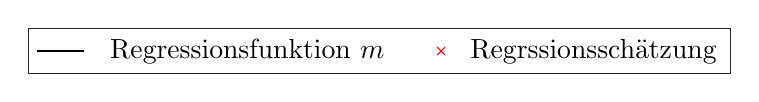
\begin{tikzpicture} 
    \begin{axis}[%
    legend columns=2,
    hide axis,
    xmin=10,
    xmax=50,
    ymin=0,
    ymax=0.4,
    legend style={draw=white!15!black,legend cell align=left,column sep=0.25cm}
    ]
    \addlegendimage{no markers,black}
    \addlegendentry{Regressionsfunktion $m \quad$};
     \addlegendimage{only marks,red,mark=x}
    \addlegendentry{Regrssionsschätzung};
    \end{axis}
\end{tikzpicture}}
    \end{subfigure}
    \caption{Approximation der Regressionsfunktion $m(x) = \sin\big(\frac{\pi}{2} \cdot x^2\big)$ durch unseren Neuronale-Netze-Regressionsschätzer mit Parametern $d = 1$, $q = 2$, $R = 10^6$, $a = 3$, $M = 2$ und $N \in \{2,4,8,16\}$.}
    \label{fig:subfig.a.1}
\end{figure}
\begin{figure}
    \begin{subfigure}[b]{0.5\textwidth}
    \centering
    \scalebox{0.9}{
	% This file was created by tikzplotlib v0.9.0.
\begin{tikzpicture}

\begin{axis}[
tick align=outside,
tick pos=left,
title={$N = 2$, $M = 2$},
x grid style={white!69.0196078431373!black},
xmin=-3.34207441715318, xmax=3.35388433148518,
xtick style={color=black},
y grid style={white!69.0196078431373!black},
ymin=\ymin, ymax=\ymax,
ytick style={color=black}
]
\addplot [only marks, mark=x, draw=red, fill=red, colormap/viridis]
table{%
x                      y
2.76238288932011 0.0696236318238279
-2.97867143721344 0.633737080000907
1.34016626636584 0.248714554967007
-2.34602979642214 -0.182357969914886
0.262724949982951 0.276579929762546
0.761496100082008 0.579943587033136
-1.54231724537519 0.137487826890353
2.48306325147965 -0.209050168109025
0.733875172149707 0.581862620438073
-1.60983185163084 0.0944463650714438
1.62079312559885 0.0128238998441449
-2.36695752001599 -0.169806042172586
0.331351911188067 0.366935291492553
-2.43026358118505 -0.148779202921674
0.485904436050117 0.50608690784783
-1.48211932367887 0.182067639405539
0.896800847728478 0.540051784810156
1.29496171714908 0.303477121481799
0.145113687411967 0.0773410376422204
0.945128446218661 0.524945754879947
1.87976307195033 -0.191036365260491
1.84507362985819 -0.133432065216717
0.718091952323177 0.570885589137396
-0.293385227275351 0.310656856937984
-0.552300065715795 0.51805352131015
2.24848571942618 -0.281705380200185
1.21759039268623 0.345041357964498
-1.89038986575959 -0.110954426485695
0.39439287977558 0.42502169868815
2.45284819380034 -0.291049415195146
-2.09586004651037 -0.174790102547986
2.07310605318424 -0.258593913584902
1.9212147978921 -0.20819892091787
-0.00395339221299285 -0.213846884924733
-2.77449689108578 0.221864318492094
-2.11498496761839 -0.189604387705741
2.53583216813203 -0.186964112299095
-2.73507122380883 0.152535754337504
-0.765007401567843 0.567667271209152
0.714237808352825 0.574790029524826
-1.8183117665159 -0.0678797541792888
2.88647854344178 0.328580875841696
-2.06414860173947 -0.197580498970857
0.238075170967647 0.234706842829697
0.708067946079868 0.563210486112765
-1.61406030798178 0.0824455711739863
-0.202146064743951 0.181958653527321
-0.0539488252024247 -0.106001454253169
1.60117425795925 0.0268839866227892
0.80568451664324 0.569994864268828
-0.194699681607962 0.155109836510655
1.00165525916385 0.493954542768638
-0.27973544086681 0.289157685130155
0.154269548048458 0.0956456982377724
0.951408249350171 0.520713845991454
-1.91282770827683 -0.127397947271127
1.72829730703384 -0.0981881929027961
0.617192025230384 0.55205086222802
2.88199731082397 0.257672602530644
-1.66570083881295 0.0289289295878304
-0.202401155000559 0.173928900889795
2.37385081559668 -0.282189394553184
0.608600458192729 0.551859514930808
1.35575307509289 0.240605729820491
-0.517979014791838 0.509784695143142
1.10585773098792 0.433697362702257
2.67633017908538 -0.0581264373606373
-1.79888360556407 -0.0548319027405837
1.84419158326392 -0.16453292485422
2.81722807259938 0.129299858654392
-2.91258760942001 0.462533316200221
-1.70874248043343 -0.00265669709421586
-2.29573847812122 -0.197860934334551
1.60454110644872 0.0123043503044086
-2.5127004843436 -0.100211621541327
2.99048135154545 0.580477883172723
-0.662327904724169 0.562940735546021
2.43121659559824 -0.261737470590812
-1.86853437900319 -0.0867912316975652
-0.354766801066255 0.377849280746422
2.06887091403722 -0.263172932170869
0.571618684039537 0.540758268586486
-0.227051419851858 0.208952653519809
0.0758984805427056 -0.0660598577993334
0.443313161354085 0.467849231283596
-0.358084754486441 0.381040306623068
-1.83864625365714 -0.0820334262989837
-2.31620543124488 -0.185655582899956
-2.09263243577911 -0.193333018106388
-2.6850542168812 0.0741495862569121
0.352058466381789 0.400423386956392
2.08632608421606 -0.282303520605454
-0.845283966455336 0.561303048771281
-2.54813476418509 -0.0782902428983408
-0.445653528089303 0.462311761039538
0.612047030832008 0.551986963974434
-0.447579206546175 0.459834061505772
1.86432740164422 -0.179658424288866
2.65131747712023 -0.0627350597311313
2.21946463961013 -0.307059454464259
1.22399698967933 0.345021100869182
-0.178206451306949 0.1319605260999
1.09618825741951 0.429667535760761
-2.91949013666082 0.488183705540907
2.89486871101226 0.352203562036919
-1.96753600902662 -0.16045119359885
2.43756237577009 -0.288929628562372
1.84265940999664 -0.161298104879786
1.80083810632193 -0.141055692020237
-1.38638365328961 0.251869349071475
-1.68507716545645 0.0246260328122515
-0.427195842515467 0.443204831149814
2.09622660438393 -0.296207948253234
-0.297722145169678 0.312538376398336
2.61252068404237 -0.134573678836577
-0.883924036489572 0.546033270670057
0.716352994180558 0.570243797957124
2.88419421813468 0.263470255215231
0.86077513344483 0.544442885926027
-2.72701070375638 0.125755209385306
-0.218657454289729 0.195394301722511
-0.991491937718017 0.505110821563645
0.193089291130048 0.171200551825321
-1.29152274832121 0.329947721561154
-2.26643261861998 -0.190159426463652
1.00973393250481 0.502298921982884
1.08815852934784 0.455020376152709
2.20283579999453 -0.285933767539575
-2.20571103862358 -0.201050492351098
1.79172184966819 -0.111927190509838
1.96061243043077 -0.219791303528054
0.879299614506912 0.545472812107093
-1.7704671253162 -0.0291843733066064
-1.43147571356497 0.227746932556877
-0.489019094764946 0.487883854119478
0.250794436696388 0.274569478277348
-0.135372266446698 0.0500974715983145
-0.195240647727783 0.162354897047872
2.039044261186 -0.292797146638685
2.22061419184541 -0.287449503098603
1.9005237862606 -0.192106090073864
2.2668085118082 -0.274119117160396
0.426052571622439 0.44960618800233
2.78421680003449 0.140845652944863
0.639266089502806 0.572103220112891
0.623686446478088 0.553399251051943
-1.08421357755229 0.460697208765001
1.08722510470211 0.450440988578061
-2.68820586896783 0.0913492374542259
-2.19272147392835 -0.199964350161324
-2.21854699456341 -0.202163173332134
0.931207723348414 0.52067877587295
-1.94800444937197 -0.153516583129393
-0.953119060490716 0.52563240549111
-2.73413006500137 0.165634437169029
-1.59759383930094 0.086424839086587
2.78534594909577 0.142258860244893
0.0548364150982064 -0.0927990326237934
-2.09355288917141 -0.193557648022957
0.138051190406785 0.0789920873749814
2.66105630346648 -0.0658396521506408
2.194116084038 -0.295449086285518
-0.647604786417679 0.564919032371968
-1.29679490415958 0.313336184944381
1.57037917615645 0.0221899214320187
-1.55709405118147 0.121053137557245
-1.47460587205589 0.180047593251032
-2.49548187492042 -0.117716440387838
2.18486456858416 -0.330379017657128
-0.312606506278321 0.34142705463999
0.370717563659841 0.409033019659376
1.42026574616112 0.160195775442276
1.77893320278717 -0.109328186028923
-0.314951166058117 0.333188366110346
-1.89523466294521 -0.111587123211569
1.97239710916981 -0.220964999610406
-2.81401224103046 0.273043906979287
2.68036961764771 -0.0263855368729497
0.461867078865009 0.487366450058124
2.25233243070412 -0.302674491559908
0.651392621841352 0.565401484012899
-1.49004249508606 0.187522044760347
-1.22322045902457 0.368519554333596
0.197535354189919 0.18369781959133
2.77246927708256 0.0889320961106456
-1.89302637305893 -0.112964568570176
0.0593902688586541 -0.082299678630407
-0.937271379378934 0.530946198776765
1.61835206974311 0.0172177591909828
1.81719891859454 -0.147646715163199
-0.4526405381867 0.455338576591202
-1.77526500003398 -0.0287151264295879
-2.59746323802687 -0.0327566121202083
-1.80811041347663 -0.0564382347081382
-1.36559489922371 0.274966941442125
0.592733507455263 0.5512862734667
2.23850098364661 -0.301633261716772
-2.23061436692708 -0.202017047050301
2.74913245028938 -0.0145682835209204
1.09902506312488 0.438680147808397
};
\addplot [semithick, black]
table {%
-3 1
-2.99 0.995576734820054
-2.98 0.982404791977482
-2.97 0.960687140310815
-2.96 0.930698746339696
-2.95 0.892782465918225
-2.94 0.847344438774256
-2.93 0.794849046139829
-2.92 0.735813493407208
-2.91 0.670802080787205
-2.9 0.6004202253259
-2.89 0.525308297382294
-2.88 0.446135333817727
-2.87 0.363592688736647
-2.86 0.278387680690676
-2.85 0.191237292858769
-2.84 0.102861979893671
-2.83 0.0139796319282911
-2.82 -0.0747002572851044
-2.81 -0.162482174923344
-2.8 -0.248689887164819
-2.79 -0.332671415810564
-2.78 -0.413803662790115
-2.77 -0.491496656276015
-2.76000000000001 -0.565197396549224
-2.75000000000001 -0.63439328416361
-2.74000000000001 -0.698615117310616
-2.73000000000001 -0.7574396495474
-2.72000000000001 -0.810491703188593
-2.71000000000001 -0.857445837641644
-2.70000000000001 -0.898027575760592
-2.69000000000001 -0.932014194877928
-2.68000000000001 -0.959235092527838
-2.67000000000001 -0.979571739978357
-2.66000000000001 -0.992957239530362
-2.65000000000001 -0.999375504106505
-2.64000000000001 -0.998860079935072
-2.63000000000001 -0.991492635127341
-2.62000000000001 -0.977401138650261
-2.61000000000001 -0.956757755609883
-2.60000000000001 -0.929776485888277
-2.59000000000001 -0.896710574023413
-2.58000000000001 -0.857849718795458
-2.57000000000001 -0.813517111294285
-2.56000000000001 -0.764066330303094
-2.55000000000001 -0.709878123655345
-2.54000000000001 -0.651357103821107
-2.53000000000001 -0.588928385370132
-2.52000000000001 -0.523034191158988
-2.51000000000001 -0.454130453115695
-2.50000000000001 -0.382683432365167
-2.49000000000001 -0.309166382170306
-2.48000000000001 -0.234056275775223
-2.47000000000001 -0.157830619746354
-2.46000000000001 -0.0809643718325892
-2.45000000000001 -0.00392698072389465
-2.44000000000001 0.072820436603254
-2.43000000000001 0.148827765990005
-2.42000000000001 0.223658403427451
-2.41000000000001 0.296891588141009
-2.40000000000001 0.368124552684589
-2.39000000000001 0.43697448301218
-2.38000000000001 0.503080283168017
-2.37000000000001 0.56610414086275
-2.36000000000001 0.625732891772279
-2.35000000000001 0.681679181898872
-2.34000000000001 0.733682428763456
-2.33000000000001 0.781509583546624
-2.32000000000001 0.824955697558263
-2.31000000000001 0.863844297587357
-2.30000000000001 0.898027575760569
-2.29000000000002 0.927386400518292
-2.28000000000002 0.951830156198068
-2.27000000000002 0.971296419496836
-2.26000000000002 0.985750481765479
-2.25000000000002 0.995184726672186
-2.24000000000002 0.999617873256875
-2.23000000000002 0.999094094789406
-2.22000000000002 0.993682024142277
-2.21000000000002 0.983473656597255
-2.20000000000002 0.96858316112866
-2.19000000000002 0.949145611247931
-2.18000000000002 0.925315646459183
-2.17000000000002 0.897266075268519
-2.16000000000002 0.865186430515806
-2.15000000000002 0.829281487561826
-2.14000000000002 0.789769755571343
-2.13000000000002 0.746881951789148
-2.12000000000002 0.700859468316991
-2.11000000000002 0.651952840469899
-2.10000000000002 0.600420225325985
-2.09000000000002 0.546525898589853
-2.08000000000002 0.490538777371198
-2.07000000000002 0.432730975942088
-2.06000000000002 0.373376400983612
-2.05000000000002 0.31274939226965
-2.04000000000002 0.251123414166708
-2.03000000000002 0.188769802758421
-2.02000000000002 0.125956572835066
-2.01000000000002 0.062947288426061
-2.00000000000002 1.33870012014889e-13
-1.99000000000002 -0.062633749083271
-1.98000000000002 -0.124709844813965
-1.97000000000002 -0.185992451913749
-1.96000000000002 -0.246254789302508
-1.95000000000002 -0.305279831055913
-1.94000000000002 -0.3628609327075
-1.93000000000002 -0.418802383167873
-1.92000000000002 -0.472919882928091
-1.91000000000002 -0.525040949582032
-1.90000000000002 -0.575005252043164
-1.89000000000002 -0.622664875144035
-1.88000000000002 -0.667884516592001
-1.87000000000002 -0.710541618511978
-1.86000000000002 -0.750526436036607
-1.85000000000002 -0.787742045606543
-1.84000000000002 -0.822104295818981
-1.83000000000002 -0.85354170381174
-1.82000000000003 -0.881995300293982
-1.81000000000003 -0.907418426433774
-1.80000000000003 -0.929776485888198
-1.79000000000003 -0.949046655314642
-1.78000000000003 -0.965217556733346
-1.77000000000003 -0.978288895122437
-1.76000000000003 -0.988271064618766
-1.75000000000003 -0.995184726672183
-1.74000000000003 -0.99906036345861
-1.73000000000003 -0.999937809799883
-1.72000000000003 -0.997865766766904
-1.71000000000003 -0.992901300058717
-1.70000000000003 -0.985109326154799
-1.69000000000003 -0.974562089132473
-1.68000000000003 -0.961338630927184
-1.67000000000003 -0.945524257691589
-1.66000000000003 -0.92721000478115
-1.65000000000003 -0.906492102760418
-1.64000000000003 -0.883471446686396
-1.63000000000003 -0.858253070784441
-1.62000000000003 -0.830945630488965
-1.61000000000003 -0.801660893676759
-1.60000000000003 -0.770513242775885
-1.59000000000003 -0.737619189288572
-1.58000000000003 -0.703096902123257
-1.57000000000003 -0.667065750989361
-1.56000000000003 -0.629645865969377
-1.55000000000003 -0.590957714246878
-1.54000000000003 -0.5511216948366
-1.53000000000003 -0.510257752034371
-1.52000000000003 -0.468485008180726
-1.51000000000003 -0.425921416212823
-1.50000000000003 -0.382683432365229
-1.49000000000003 -0.338885709271396
-1.48000000000003 -0.29464080961443
-1.47000000000003 -0.250058940378286
-1.46000000000003 -0.205247707658841
-1.45000000000003 -0.16031189190854
-1.44000000000003 -0.115353243408457
-1.43000000000003 -0.0704702976877775
-1.42000000000003 -0.0257582105426693
-1.41000000000003 0.018691387755514
-1.40000000000003 0.0627905195291638
-1.39000000000003 0.106454968557562
-1.38000000000003 0.149604371296494
-1.37000000000003 0.192162291056312
-1.36000000000003 0.234056275774993
-1.35000000000004 0.275217900052248
-1.34000000000004 0.315582792135412
-1.33000000000004 0.355090646567928
-1.32000000000004 0.393685223226887
-1.31000000000004 0.431314333487567
-1.30000000000004 0.467929814260443
-1.29000000000004 0.503487490649953
-1.28000000000004 0.537947127984647
-1.27000000000004 0.571272373965398
-1.26000000000004 0.603430691672474
-1.25000000000004 0.634393284163532
-1.24000000000004 0.664135011383361
-1.23000000000004 0.692634300092632
-1.22000000000004 0.719873047507249
-1.21000000000004 0.745836519322339
-1.20000000000004 0.770513242775697
-1.19000000000004 0.79389489538482
-1.18000000000004 0.815976189969678
-1.17000000000004 0.836754756550324
-1.16000000000004 0.856231021684473
-1.15000000000004 0.87440808578545
-1.14000000000004 0.891291598935659
-1.13000000000004 0.906889635684947
-1.12000000000004 0.921212569297285
-1.11000000000004 0.93427294588298
-1.10000000000004 0.9460853588275
-1.09000000000004 0.956666323901834
-1.08000000000004 0.966034155413461
-1.07000000000004 0.974208843731348
-1.06000000000004 0.981211934493193
-1.05000000000004 0.987066409778344
-1.04000000000004 0.991796571505593
-1.03000000000004 0.995427927291427
-1.02000000000004 0.997987078981312
-1.01000000000004 0.999501614044331
-1.00000000000004 1
-0.990000000000043 0.999511482025296
-0.980000000000043 0.998065983870084
-0.970000000000043 0.995694012190007
-0.960000000000043 0.992426564387702
-0.950000000000044 0.988295040035889
-0.940000000000044 0.983331155939389
-0.930000000000044 0.977566864877576
-0.920000000000044 0.971034278054095
-0.910000000000045 0.963765591266851
-0.900000000000045 0.955793014798367
-0.890000000000045 0.94714870701456
-0.880000000000045 0.937864711648732
-0.870000000000045 0.927972898737259
-0.860000000000046 0.917504909163832
-0.850000000000046 0.906492102760406
-0.840000000000046 0.894965509904969
-0.830000000000046 0.882955786549018
-0.820000000000046 0.870493172601118
-0.810000000000047 0.857607453587072
-0.800000000000047 0.844327925502078
-0.790000000000047 0.830683362765738
-0.780000000000047 0.816701989186866
-0.770000000000048 0.802411451841723
-0.760000000000048 0.787838797766522
-0.750000000000048 0.773010453362809
-0.740000000000048 0.757952206412552
-0.730000000000048 0.742689190598499
-0.720000000000049 0.727245872424471
-0.710000000000049 0.711646040429847
-0.700000000000049 0.695912796592392
-0.690000000000049 0.68006854981388
-0.680000000000049 0.664135011383549
-0.67000000000005 0.648133192315342
-0.66000000000005 0.632083402456062
-0.65000000000005 0.61600525126299
-0.64000000000005 0.599917650151169
-0.630000000000051 0.583838816312412
-0.620000000000051 0.567786277910133
-0.610000000000051 0.551776880556293
-0.600000000000051 0.535826794979078
-0.590000000000051 0.519951525792427
-0.580000000000052 0.504165921281037
-0.570000000000052 0.488484184117171
-0.560000000000052 0.472919882928293
-0.550000000000052 0.457485964637341
-0.540000000000052 0.442194767500267
-0.530000000000053 0.427058034768333
-0.520000000000053 0.4120869289055
-0.510000000000053 0.397292046294142
-0.500000000000053 0.382683432365167
-0.490000000000054 0.368270597091477
-0.480000000000054 0.354062530786545
-0.470000000000054 0.340067720152659
-0.460000000000054 0.326294164526146
-0.450000000000054 0.312749392269599
-0.440000000000055 0.299440477263786
-0.430000000000055 0.286374055454505
-0.420000000000055 0.273556341412193
-0.410000000000055 0.260993144864562
-0.400000000000055 0.248689887164922
-0.390000000000056 0.23665161766118
-0.380000000000056 0.22488302993274
-0.370000000000056 0.213388477864702
-0.360000000000056 0.202171991530836
-0.350000000000056 0.191237292858801
-0.340000000000057 0.180587811053027
-0.330000000000057 0.170226697752469
-0.320000000000057 0.160156841902239
-0.310000000000057 0.150380884319751
-0.300000000000058 0.140901231937636
-0.290000000000058 0.131720071707145
-0.280000000000058 0.122839384147215
-0.270000000000058 0.114260956525697
-0.260000000000058 0.105986395660502
-0.250000000000059 0.0980171403296064
-0.240000000000059 0.0903544732799798
-0.230000000000059 0.0829995328265039
-0.220000000000059 0.0759533240329385
-0.210000000000059 0.0692167294678623
-0.20000000000006 0.0627905195293508
-0.19000000000006 0.0566753623329036
-0.18000000000006 0.0508718331578319
-0.17000000000006 0.0453804234479493
-0.160000000000061 0.0402015493629836
-0.150000000000061 0.0353355598776498
-0.140000000000061 0.0307827444257893
-0.130000000000061 0.0265433400874004
-0.120000000000061 0.0226175383167529
-0.110000000000062 0.019005491210107
-0.100000000000062 0.0157073173118401
-0.090000000000062 0.012723106958029
-0.0800000000000622 0.0100529271567463
-0.0700000000000625 0.00769682600450373
-0.0600000000000627 0.00565483663842069
-0.0500000000000629 0.00392698072381588
-0.0400000000000631 0.00251327147701166
-0.0300000000000633 0.00141371622321359
-0.0200000000000635 0.000628318489380248
-0.0100000000000637 0.000157079632035528
-6.3948846218409e-14 6.42370078682459e-27
0.00999999999993584 0.00015707963203151
0.0199999999999356 0.000628318489372212
0.0299999999999354 0.00141371622320154
0.0399999999999352 0.00251327147699558
0.049999999999935 0.00392698072379579
0.0599999999999348 0.00565483663839659
0.0699999999999346 0.00769682600447561
0.0799999999999343 0.0100529271567142
0.0899999999999341 0.0127231069579928
0.0999999999999339 0.0157073173117999
0.109999999999934 0.0190054912100628
0.119999999999933 0.0226175383167047
0.129999999999933 0.0265433400873482
0.139999999999933 0.0307827444257331
0.149999999999933 0.0353355598775896
0.159999999999933 0.0402015493629194
0.169999999999932 0.045380423447881
0.179999999999932 0.0508718331577597
0.189999999999932 0.0566753623328273
0.199999999999932 0.0627905195292706
0.209999999999932 0.0692167294677781
0.219999999999931 0.0759533240328503
0.229999999999931 0.0829995328264118
0.239999999999931 0.0903544732798837
0.249999999999931 0.0980171403295065
0.259999999999931 0.105986395660398
0.26999999999993 0.114260956525589
0.27999999999993 0.122839384147103
0.28999999999993 0.131720071707029
0.29999999999993 0.140901231937517
0.309999999999929 0.150380884319628
0.319999999999929 0.160156841902112
0.329999999999929 0.170226697752338
0.339999999999929 0.180587811052893
0.349999999999929 0.191237292858663
0.359999999999928 0.202171991530694
0.369999999999928 0.213388477864557
0.379999999999928 0.224883029932591
0.389999999999928 0.236651617661028
0.399999999999928 0.248689887164767
0.409999999999927 0.260993144864403
0.419999999999927 0.273556341412031
0.429999999999927 0.28637405545434
0.439999999999927 0.299440477263618
0.449999999999926 0.312749392269427
0.459999999999926 0.326294164525971
0.469999999999926 0.340067720152481
0.479999999999926 0.354062530786364
0.489999999999926 0.368270597091294
0.499999999999925 0.382683432364981
0.509999999999925 0.397292046293954
0.519999999999925 0.412086928905309
0.529999999999925 0.42705803476814
0.539999999999925 0.442194767500072
0.549999999999924 0.457485964637144
0.559999999999924 0.472919882928095
0.569999999999924 0.488484184116971
0.579999999999924 0.504165921280836
0.589999999999923 0.519951525792225
0.599999999999923 0.535826794978874
0.609999999999923 0.551776880556088
0.619999999999923 0.567786277909928
0.629999999999923 0.583838816312206
0.639999999999922 0.599917650150963
0.649999999999922 0.616005251262785
0.659999999999922 0.632083402455857
0.669999999999922 0.648133192315137
0.679999999999922 0.664135011383345
0.689999999999921 0.680068549813677
0.699999999999921 0.69591279659219
0.709999999999921 0.711646040429646
0.719999999999921 0.727245872424273
0.72999999999992 0.742689190598303
0.73999999999992 0.757952206412358
0.74999999999992 0.773010453362617
0.75999999999992 0.787838797766334
0.76999999999992 0.802411451841539
0.779999999999919 0.816701989186685
0.789999999999919 0.830683362765561
0.799999999999919 0.844327925501906
0.809999999999919 0.857607453586905
0.819999999999919 0.870493172600956
0.829999999999918 0.882955786548861
0.839999999999918 0.894965509904818
0.849999999999918 0.906492102760262
0.859999999999918 0.917504909163694
0.869999999999918 0.927972898737128
0.879999999999917 0.93786471164861
0.889999999999917 0.947148707014445
0.899999999999917 0.955793014798261
0.909999999999917 0.963765591266753
0.919999999999916 0.971034278054007
0.929999999999916 0.977566864877497
0.939999999999916 0.98333115593932
0.949999999999916 0.988295040035831
0.959999999999916 0.992426564387655
0.969999999999915 0.995694012189971
0.979999999999915 0.99806598387006
0.989999999999915 0.999511482025283
0.999999999999915 1
1.00999999999991 0.999501614044344
1.01999999999991 0.997987078981338
1.02999999999991 0.995427927291467
1.03999999999991 0.991796571505646
1.04999999999991 0.987066409778411
1.05999999999991 0.981211934493276
1.06999999999991 0.974208843731445
1.07999999999991 0.966034155413573
1.08999999999991 0.956666323901962
1.09999999999991 0.946085358827643
1.10999999999991 0.934272945883139
1.11999999999991 0.92121256929746
1.12999999999991 0.906889635685138
1.13999999999991 0.891291598935866
1.14999999999991 0.874408085785674
1.15999999999991 0.856231021684713
1.16999999999991 0.836754756550582
1.17999999999991 0.815976189969952
1.18999999999991 0.793894895385111
1.19999999999991 0.770513242776004
1.20999999999991 0.745836519322663
1.21999999999991 0.719873047507589
1.22999999999991 0.692634300092988
1.23999999999991 0.664135011383733
1.24999999999991 0.63439328416392
1.25999999999991 0.603430691672878
1.26999999999991 0.571272373965817
1.27999999999991 0.537947127985081
1.28999999999991 0.503487490650401
1.29999999999991 0.467929814260904
1.30999999999991 0.431314333488042
1.31999999999991 0.393685223227375
1.32999999999991 0.355090646568427
1.33999999999991 0.315582792135923
1.34999999999991 0.27521790005277
1.35999999999991 0.234056275775525
1.36999999999991 0.192162291056853
1.37999999999991 0.149604371297043
1.38999999999991 0.106454968558117
1.39999999999991 0.0627905195297253
1.40999999999991 0.0186913877560805
1.41999999999991 -0.0257582105420993
1.42999999999991 -0.0704702976872039
1.43999999999991 -0.115353243407883
1.44999999999991 -0.160311891907964
1.4599999999999 -0.205247707658268
1.4699999999999 -0.250058940377715
1.4799999999999 -0.294640809613862
1.4899999999999 -0.338885709270833
1.4999999999999 -0.382683432364672
1.5099999999999 -0.425921416212274
1.5199999999999 -0.468485008180186
1.5299999999999 -0.510257752033843
1.5399999999999 -0.551121694836084
1.5499999999999 -0.590957714246376
1.5599999999999 -0.62964586596889
1.5699999999999 -0.667065750988891
1.5799999999999 -0.703096902122806
1.5899999999999 -0.73761918928814
1.5999999999999 -0.770513242775475
1.6099999999999 -0.801660893676373
1.6199999999999 -0.830945630488602
1.6299999999999 -0.858253070784105
1.6399999999999 -0.883471446686087
1.6499999999999 -0.906492102760138
1.6599999999999 -0.9272100047809
1.6699999999999 -0.945524257691371
1.6799999999999 -0.961338630926998
1.6899999999999 -0.974562089132321
1.6999999999999 -0.985109326154682
1.7099999999999 -0.992901300058635
1.7199999999999 -0.997865766766859
1.7299999999999 -0.999937809799876
1.7399999999999 -0.99906036345864
1.7499999999999 -0.995184726672251
1.7599999999999 -0.988271064618874
1.7699999999999 -0.978288895122584
1.7799999999999 -0.965217556733533
1.7899999999999 -0.949046655314868
1.7999999999999 -0.929776485888465
1.8099999999999 -0.90741842643408
1.8199999999999 -0.881995300294327
1.8299999999999 -0.853541703812123
1.8399999999999 -0.822104295819402
1.8499999999999 -0.787742045607001
1.8599999999999 -0.750526436037101
1.8699999999999 -0.710541618512508
1.8799999999999 -0.667884516592564
1.8899999999999 -0.622664875144629
1.8999999999999 -0.575005252043788
1.9099999999999 -0.525040949582685
1.9199999999999 -0.47291988292877
1.92999999999989 -0.418802383168577
1.93999999999989 -0.362860932708227
1.94999999999989 -0.305279831056659
1.95999999999989 -0.246254789303272
1.96999999999989 -0.185992451914526
1.97999999999989 -0.124709844814754
1.98999999999989 -0.0626337490840697
1.99999999999989 -6.69931457813724e-13
2.00999999999989 0.0629472884252544
2.01999999999989 0.12595657283426
2.02999999999989 0.18876980275762
2.03999999999989 0.251123414165916
2.04999999999989 0.312749392268867
2.05999999999989 0.373376400982844
2.06999999999989 0.432730975941339
2.07999999999989 0.490538777370471
2.08999999999989 0.54652589858915
2.09999999999989 0.600420225325311
2.10999999999989 0.651952840469257
2.11999999999989 0.700859468316383
2.12999999999989 0.746881951788579
2.13999999999989 0.789769755570817
2.14999999999989 0.829281487561343
2.15999999999989 0.865186430515371
2.16999999999989 0.897266075268134
2.17999999999989 0.925315646458851
2.18999999999989 0.949145611247653
2.19999999999989 0.968583161128441
2.20999999999989 0.983473656597094
2.21999999999989 0.993682024142177
2.22999999999989 0.999094094789368
2.23999999999989 0.9996178732569
2.24999999999989 0.995184726672274
2.25999999999989 0.985750481765632
2.26999999999989 0.971296419497053
2.27999999999989 0.951830156198348
2.28999999999989 0.927386400518636
2.29999999999989 0.898027575760974
2.30999999999989 0.863844297587825
2.31999999999989 0.82495569755879
2.32999999999989 0.781509583547208
2.33999999999989 0.733682428764095
2.34999999999989 0.681679181899562
2.35999999999989 0.625732891773019
2.36999999999989 0.566104140863535
2.37999999999989 0.503080283168843
2.38999999999989 0.436974483013044
2.39999999999988 0.368124552685486
2.40999999999988 0.296891588141934
2.41999999999988 0.2236584034284
2.42999999999988 0.148827765990971
2.43999999999988 0.072820436604232
2.44999999999988 -0.00392698072291233
2.45999999999988 -0.0809643718316048
2.46999999999988 -0.157830619745374
2.47999999999988 -0.234056275774253
2.48999999999988 -0.309166382169355
2.49999999999988 -0.382683432364238
2.50999999999988 -0.454130453114798
2.51999999999988 -0.523034191158123
2.52999999999988 -0.58892838536931
2.53999999999988 -0.651357103820333
2.54999999999988 -0.709878123654623
2.55999999999988 -0.764066330302429
2.56999999999988 -0.813517111293685
2.57999999999988 -0.857849718794925
2.58999999999988 -0.896710574022952
2.59999999999988 -0.929776485887892
2.60999999999988 -0.956757755609577
2.61999999999988 -0.977401138650039
2.62999999999988 -0.991492635127203
2.63999999999988 -0.998860079935021
2.64999999999988 -0.999375504106543
2.65999999999988 -0.992957239530489
2.66999999999988 -0.979571739978573
2.67999999999988 -0.959235092528142
2.68999999999988 -0.93201419487832
2.69999999999988 -0.898027575761069
2.70999999999988 -0.857445837642205
2.71999999999988 -0.810491703189233
2.72999999999988 -0.757439649548115
2.73999999999988 -0.698615117311402
2.74999999999988 -0.634393284164464
2.75999999999988 -0.565197396550139
2.76999999999988 -0.491496656276984
2.77999999999988 -0.413803662791132
2.78999999999988 -0.332671415811622
2.79999999999988 -0.248689887165909
2.80999999999988 -0.162482174924459
2.81999999999988 -0.0747002572862345
2.82999999999988 0.0139796319271562
2.83999999999988 0.102861979892536
2.84999999999988 0.191237292857646
2.85999999999988 0.278387680689572
2.86999999999987 0.36359268873557
2.87999999999987 0.44613533381669
2.88999999999987 0.525308297381304
2.89999999999987 0.600420225324967
2.90999999999987 0.670802080786339
2.91999999999987 0.735813493406414
2.92999999999987 0.794849046139114
2.93999999999987 0.847344438773628
2.94999999999987 0.892782465917691
2.95999999999987 0.930698746339261
2.96999999999987 0.960687140310484
2.97999999999987 0.982404791977258
2.98999999999987 0.995576734819941
};
\end{axis}

\end{tikzpicture}
}
        \label{fig:subfig2n2m2}
    \end{subfigure}
    \begin{subfigure}[b]{0.5\textwidth}
    \centering
     \scalebox{0.9}{
           % This file was created by tikzplotlib v0.9.0.
\begin{tikzpicture}

\begin{axis}[
tick align=outside,
tick pos=left,
title={$N = 2$, $M = 4$},
x grid style={white!69.0196078431373!black},
xmin=-3.34207441715318, xmax=3.35388433148518,
xtick style={color=black},
y grid style={white!69.0196078431373!black},
ymin=\ymin, ymax=\ymax,
ytick style={color=black}
]
\addplot [only marks, mark=x, draw=red, fill=red, colormap/viridis]
table{%
x                      y
2.76238288932011 0.0548573361516268
-2.97867143721344 0.39004246210036
1.34016626636584 0.193882688735216
-2.34602979642214 0.113977977161504
0.262724949982951 0.0600015805971778
0.761496100082008 0.841171021419397
-1.54231724537519 -0.789681119456945
2.48306325147965 -0.0621537053009609
0.733875172149707 0.803448480688595
-1.60983185163084 -0.622834727971975
1.62079312559885 -0.507147052603633
-2.36695752001599 0.108629140535199
0.331351911188067 0.0967534008267986
-2.43026358118505 0.124686088361745
0.485904436050117 0.335397230983933
-1.48211932367887 -0.757321989549028
0.896800847728478 1.04022991250867
1.29496171714908 0.447289011441023
0.145113687411967 0.0272741941538612
0.945128446218661 1.04645348841622
1.87976307195033 -0.191155390960763
1.84507362985819 -0.189096561733417
0.718091952323177 0.721481310395205
-0.293385227275351 0.0441655670415681
-0.552300065715795 0.460095666875378
2.24848571942618 0.0134680283338148
1.21759039268623 0.685844648414252
-1.89038986575959 -0.13911672232947
0.39439287977558 0.175423619287281
2.45284819380034 0.0382848635317306
-2.09586004651037 0.0231300091690418
2.07310605318424 -0.0567594082002973
1.9212147978921 -0.109400244076076
-0.00395339221299285 0.189158609729156
-2.77449689108578 0.223841864036341
-2.11498496761839 0.0458351246207127
2.53583216813203 -0.105973353612043
-2.73507122380883 0.20396477489076
-0.765007401567843 0.880141991557563
0.714237808352825 0.762982129278016
-1.8183117665159 -0.229036022853851
2.88647854344178 0.279063214838452
-2.06414860173947 0.00705854901561175
0.238075170967647 -0.00472963274343371
0.708067946079868 0.77882074040996
-1.61406030798178 -0.608367927428695
-0.202146064743951 -0.00417859644671259
-0.0539488252024247 0.100059781766365
1.60117425795925 -0.551762398550337
0.80568451664324 0.857477912796351
-0.194699681607962 -0.0190271697058804
1.00165525916385 1.02113138955927
-0.27973544086681 0.0374825496844748
0.154269548048458 0.00849892468457938
0.951408249350171 0.998253477928714
-1.91282770827683 -0.109529244699241
1.72829730703384 -0.317416425382685
0.617192025230384 0.591494031193033
2.88199731082397 0.0979963838895313
-1.66570083881295 -0.494041938980318
-0.202401155000559 -0.00953147848118279
2.37385081559668 -0.100410115338715
0.608600458192729 0.560966127117591
1.35575307509289 0.115879475857676
-0.517979014791838 0.39767607949715
1.10585773098792 0.896703482854145
2.67633017908538 -0.0661419943622875
-1.79888360556407 -0.260461755426478
1.84419158326392 -0.127661156923801
2.81722807259938 0.0715787980639901
-2.91258760942001 0.313442579530375
-1.70874248043343 -0.407002125654337
-2.29573847812122 0.10336901816239
1.60454110644872 -0.510371772085304
-2.5127004843436 0.13095553051482
2.99048135154545 0.325184279668299
-0.662327904724169 0.67756680802431
2.43121659559824 0.106385440149971
-1.86853437900319 -0.163795999210191
-0.354766801066255 0.108906163837406
2.06887091403722 -0.129885398433247
0.571618684039537 0.523905909865923
-0.227051419851858 0.00801676613984355
0.0758984805427056 0.0836807150145017
0.443313161354085 0.253708514014559
-0.358084754486441 0.0926368006883695
-1.83864625365714 -0.203447568092537
-2.31620543124488 0.101182221243597
-2.09263243577911 0.0227302339416998
-2.6850542168812 0.185451937614085
0.352058466381789 0.110158184666202
2.08632608421606 -0.116262571769781
-0.845283966455336 0.981840088620561
-2.54813476418509 0.140974164765658
-0.445653528089303 0.258753770430353
0.612047030832008 0.58234246599914
-0.447579206546175 0.260082001368176
1.86432740164422 -0.173192670366243
2.65131747712023 -0.0293560427621832
2.21946463961013 -0.00944214125589141
1.22399698967933 0.650334354819754
-0.178206451306949 -0.0346576880196753
1.09618825741951 0.934465830661224
-2.91949013666082 0.324349574292963
2.89486871101226 0.0737482303534916
-1.96753600902662 -0.0602331632879468
2.43756237577009 -0.0348996238823714
1.84265940999664 -0.154881989043999
1.80083810632193 -0.233662740331947
-1.38638365328961 -0.0745969158806232
-1.68507716545645 -0.461687240231081
-0.427195842515467 0.209118752367969
2.09622660438393 -0.0765874999482647
-0.297722145169678 0.0473985763461933
2.61252068404237 0.000674635985736402
-0.883924036489572 1.01289159540991
0.716352994180558 0.811437636342553
2.88419421813468 0.111793357917585
0.86077513344483 0.992217448938961
-2.72701070375638 0.19453682541522
-0.218657454289729 -0.015351587277294
-0.991491937718017 1.05921240412247
0.193089291130048 0.0072817777136472
-1.29152274832121 0.431816673771424
-2.26643261861998 0.0804079711727146
1.00973393250481 1.03101957108268
1.08815852934784 0.977693462759781
2.20283579999453 -0.0388823045029999
-2.20571103862358 0.071373277078349
1.79172184966819 -0.278289707322954
1.96061243043077 -0.0905992544104142
0.879299614506912 0.975635019597465
-1.7704671253162 -0.299630716504698
-1.43147571356497 -0.37447145934739
-0.489019094764946 0.339101959978666
0.250794436696388 0.0321848550402938
-0.135372266446698 0.0208518022564523
-0.195240647727783 0.00958698365860234
2.039044261186 -0.0862697715184539
2.22061419184541 -0.0164596438606059
1.9005237862606 -0.158925717578258
2.2668085118082 0.0357547967028564
0.426052571622439 0.267285677592055
2.78421680003449 0.103700732116476
0.639266089502806 0.608072654729986
0.623686446478088 0.580964248416975
-1.08421357755229 1.003096484996
1.08722510470211 0.972341315628371
-2.68820586896783 0.184193334265609
-2.19272147392835 0.071854639083694
-2.21854699456341 0.0819973423902437
0.931207723348414 0.990133589943155
-1.94800444937197 -0.0767911662630886
-0.953119060490716 1.04760067487243
-2.73413006500137 0.203351093282928
-1.59759383930094 -0.644702036474756
2.78534594909577 0.067444905243397
0.0548364150982064 0.111904122635227
-2.09355288917141 0.0328088603334599
0.138051190406785 0.0355300270031477
2.66105630346648 -0.045799952692099
2.194116084038 0.0152201612151816
-0.647604786417679 0.647604572030946
-1.29679490415958 0.408637795557797
1.57037917615645 -0.614474661660347
-1.55709405118147 -0.752353061863218
-1.47460587205589 -0.707918547293941
-2.49548187492042 0.128568460852907
2.18486456858416 0.0391118804981748
-0.312606506278321 0.0583166751576653
0.370717563659841 0.149213730084999
1.42026574616112 -0.284493296994157
1.77893320278717 -0.217879998443931
-0.314951166058117 0.0699694423597324
-1.89523466294521 -0.134992045930781
1.97239710916981 -0.00703925383453524
-2.81401224103046 0.244826652539472
2.68036961764771 -0.0826478654244574
0.461867078865009 0.301932412831713
2.25233243070412 -0.0251887116284929
0.651392621841352 0.674583974394901
-1.49004249508606 -0.831964992772031
-1.22322045902457 0.699103738326865
0.197535354189919 0.0110006446712176
2.77246927708256 -0.148020608554747
-1.89302637305893 -0.136925258420798
0.0593902688586541 0.0987076022450386
-0.937271379378934 1.06424099834567
1.61835206974311 -0.546705718294183
1.81719891859454 -0.222675803037026
-0.4526405381867 0.274148282337058
-1.77526500003398 -0.289162290352621
-2.59746323802687 0.16054935536666
-1.80811041347663 -0.245299754070832
-1.36559489922371 0.0587032907870236
0.592733507455263 0.557014406713278
2.23850098364661 -0.0682109783289568
-2.23061436692708 0.0822264056503658
2.74913245028938 -0.0266919119066284
1.09902506312488 0.947146712390984
};
\addplot [semithick, black]
table {%
-3 1
-2.99 0.995576734820054
-2.98 0.982404791977482
-2.97 0.960687140310815
-2.96 0.930698746339696
-2.95 0.892782465918225
-2.94 0.847344438774256
-2.93 0.794849046139829
-2.92 0.735813493407208
-2.91 0.670802080787205
-2.9 0.6004202253259
-2.89 0.525308297382294
-2.88 0.446135333817727
-2.87 0.363592688736647
-2.86 0.278387680690676
-2.85 0.191237292858769
-2.84 0.102861979893671
-2.83 0.0139796319282911
-2.82 -0.0747002572851044
-2.81 -0.162482174923344
-2.8 -0.248689887164819
-2.79 -0.332671415810564
-2.78 -0.413803662790115
-2.77 -0.491496656276015
-2.76000000000001 -0.565197396549224
-2.75000000000001 -0.63439328416361
-2.74000000000001 -0.698615117310616
-2.73000000000001 -0.7574396495474
-2.72000000000001 -0.810491703188593
-2.71000000000001 -0.857445837641644
-2.70000000000001 -0.898027575760592
-2.69000000000001 -0.932014194877928
-2.68000000000001 -0.959235092527838
-2.67000000000001 -0.979571739978357
-2.66000000000001 -0.992957239530362
-2.65000000000001 -0.999375504106505
-2.64000000000001 -0.998860079935072
-2.63000000000001 -0.991492635127341
-2.62000000000001 -0.977401138650261
-2.61000000000001 -0.956757755609883
-2.60000000000001 -0.929776485888277
-2.59000000000001 -0.896710574023413
-2.58000000000001 -0.857849718795458
-2.57000000000001 -0.813517111294285
-2.56000000000001 -0.764066330303094
-2.55000000000001 -0.709878123655345
-2.54000000000001 -0.651357103821107
-2.53000000000001 -0.588928385370132
-2.52000000000001 -0.523034191158988
-2.51000000000001 -0.454130453115695
-2.50000000000001 -0.382683432365167
-2.49000000000001 -0.309166382170306
-2.48000000000001 -0.234056275775223
-2.47000000000001 -0.157830619746354
-2.46000000000001 -0.0809643718325892
-2.45000000000001 -0.00392698072389465
-2.44000000000001 0.072820436603254
-2.43000000000001 0.148827765990005
-2.42000000000001 0.223658403427451
-2.41000000000001 0.296891588141009
-2.40000000000001 0.368124552684589
-2.39000000000001 0.43697448301218
-2.38000000000001 0.503080283168017
-2.37000000000001 0.56610414086275
-2.36000000000001 0.625732891772279
-2.35000000000001 0.681679181898872
-2.34000000000001 0.733682428763456
-2.33000000000001 0.781509583546624
-2.32000000000001 0.824955697558263
-2.31000000000001 0.863844297587357
-2.30000000000001 0.898027575760569
-2.29000000000002 0.927386400518292
-2.28000000000002 0.951830156198068
-2.27000000000002 0.971296419496836
-2.26000000000002 0.985750481765479
-2.25000000000002 0.995184726672186
-2.24000000000002 0.999617873256875
-2.23000000000002 0.999094094789406
-2.22000000000002 0.993682024142277
-2.21000000000002 0.983473656597255
-2.20000000000002 0.96858316112866
-2.19000000000002 0.949145611247931
-2.18000000000002 0.925315646459183
-2.17000000000002 0.897266075268519
-2.16000000000002 0.865186430515806
-2.15000000000002 0.829281487561826
-2.14000000000002 0.789769755571343
-2.13000000000002 0.746881951789148
-2.12000000000002 0.700859468316991
-2.11000000000002 0.651952840469899
-2.10000000000002 0.600420225325985
-2.09000000000002 0.546525898589853
-2.08000000000002 0.490538777371198
-2.07000000000002 0.432730975942088
-2.06000000000002 0.373376400983612
-2.05000000000002 0.31274939226965
-2.04000000000002 0.251123414166708
-2.03000000000002 0.188769802758421
-2.02000000000002 0.125956572835066
-2.01000000000002 0.062947288426061
-2.00000000000002 1.33870012014889e-13
-1.99000000000002 -0.062633749083271
-1.98000000000002 -0.124709844813965
-1.97000000000002 -0.185992451913749
-1.96000000000002 -0.246254789302508
-1.95000000000002 -0.305279831055913
-1.94000000000002 -0.3628609327075
-1.93000000000002 -0.418802383167873
-1.92000000000002 -0.472919882928091
-1.91000000000002 -0.525040949582032
-1.90000000000002 -0.575005252043164
-1.89000000000002 -0.622664875144035
-1.88000000000002 -0.667884516592001
-1.87000000000002 -0.710541618511978
-1.86000000000002 -0.750526436036607
-1.85000000000002 -0.787742045606543
-1.84000000000002 -0.822104295818981
-1.83000000000002 -0.85354170381174
-1.82000000000003 -0.881995300293982
-1.81000000000003 -0.907418426433774
-1.80000000000003 -0.929776485888198
-1.79000000000003 -0.949046655314642
-1.78000000000003 -0.965217556733346
-1.77000000000003 -0.978288895122437
-1.76000000000003 -0.988271064618766
-1.75000000000003 -0.995184726672183
-1.74000000000003 -0.99906036345861
-1.73000000000003 -0.999937809799883
-1.72000000000003 -0.997865766766904
-1.71000000000003 -0.992901300058717
-1.70000000000003 -0.985109326154799
-1.69000000000003 -0.974562089132473
-1.68000000000003 -0.961338630927184
-1.67000000000003 -0.945524257691589
-1.66000000000003 -0.92721000478115
-1.65000000000003 -0.906492102760418
-1.64000000000003 -0.883471446686396
-1.63000000000003 -0.858253070784441
-1.62000000000003 -0.830945630488965
-1.61000000000003 -0.801660893676759
-1.60000000000003 -0.770513242775885
-1.59000000000003 -0.737619189288572
-1.58000000000003 -0.703096902123257
-1.57000000000003 -0.667065750989361
-1.56000000000003 -0.629645865969377
-1.55000000000003 -0.590957714246878
-1.54000000000003 -0.5511216948366
-1.53000000000003 -0.510257752034371
-1.52000000000003 -0.468485008180726
-1.51000000000003 -0.425921416212823
-1.50000000000003 -0.382683432365229
-1.49000000000003 -0.338885709271396
-1.48000000000003 -0.29464080961443
-1.47000000000003 -0.250058940378286
-1.46000000000003 -0.205247707658841
-1.45000000000003 -0.16031189190854
-1.44000000000003 -0.115353243408457
-1.43000000000003 -0.0704702976877775
-1.42000000000003 -0.0257582105426693
-1.41000000000003 0.018691387755514
-1.40000000000003 0.0627905195291638
-1.39000000000003 0.106454968557562
-1.38000000000003 0.149604371296494
-1.37000000000003 0.192162291056312
-1.36000000000003 0.234056275774993
-1.35000000000004 0.275217900052248
-1.34000000000004 0.315582792135412
-1.33000000000004 0.355090646567928
-1.32000000000004 0.393685223226887
-1.31000000000004 0.431314333487567
-1.30000000000004 0.467929814260443
-1.29000000000004 0.503487490649953
-1.28000000000004 0.537947127984647
-1.27000000000004 0.571272373965398
-1.26000000000004 0.603430691672474
-1.25000000000004 0.634393284163532
-1.24000000000004 0.664135011383361
-1.23000000000004 0.692634300092632
-1.22000000000004 0.719873047507249
-1.21000000000004 0.745836519322339
-1.20000000000004 0.770513242775697
-1.19000000000004 0.79389489538482
-1.18000000000004 0.815976189969678
-1.17000000000004 0.836754756550324
-1.16000000000004 0.856231021684473
-1.15000000000004 0.87440808578545
-1.14000000000004 0.891291598935659
-1.13000000000004 0.906889635684947
-1.12000000000004 0.921212569297285
-1.11000000000004 0.93427294588298
-1.10000000000004 0.9460853588275
-1.09000000000004 0.956666323901834
-1.08000000000004 0.966034155413461
-1.07000000000004 0.974208843731348
-1.06000000000004 0.981211934493193
-1.05000000000004 0.987066409778344
-1.04000000000004 0.991796571505593
-1.03000000000004 0.995427927291427
-1.02000000000004 0.997987078981312
-1.01000000000004 0.999501614044331
-1.00000000000004 1
-0.990000000000043 0.999511482025296
-0.980000000000043 0.998065983870084
-0.970000000000043 0.995694012190007
-0.960000000000043 0.992426564387702
-0.950000000000044 0.988295040035889
-0.940000000000044 0.983331155939389
-0.930000000000044 0.977566864877576
-0.920000000000044 0.971034278054095
-0.910000000000045 0.963765591266851
-0.900000000000045 0.955793014798367
-0.890000000000045 0.94714870701456
-0.880000000000045 0.937864711648732
-0.870000000000045 0.927972898737259
-0.860000000000046 0.917504909163832
-0.850000000000046 0.906492102760406
-0.840000000000046 0.894965509904969
-0.830000000000046 0.882955786549018
-0.820000000000046 0.870493172601118
-0.810000000000047 0.857607453587072
-0.800000000000047 0.844327925502078
-0.790000000000047 0.830683362765738
-0.780000000000047 0.816701989186866
-0.770000000000048 0.802411451841723
-0.760000000000048 0.787838797766522
-0.750000000000048 0.773010453362809
-0.740000000000048 0.757952206412552
-0.730000000000048 0.742689190598499
-0.720000000000049 0.727245872424471
-0.710000000000049 0.711646040429847
-0.700000000000049 0.695912796592392
-0.690000000000049 0.68006854981388
-0.680000000000049 0.664135011383549
-0.67000000000005 0.648133192315342
-0.66000000000005 0.632083402456062
-0.65000000000005 0.61600525126299
-0.64000000000005 0.599917650151169
-0.630000000000051 0.583838816312412
-0.620000000000051 0.567786277910133
-0.610000000000051 0.551776880556293
-0.600000000000051 0.535826794979078
-0.590000000000051 0.519951525792427
-0.580000000000052 0.504165921281037
-0.570000000000052 0.488484184117171
-0.560000000000052 0.472919882928293
-0.550000000000052 0.457485964637341
-0.540000000000052 0.442194767500267
-0.530000000000053 0.427058034768333
-0.520000000000053 0.4120869289055
-0.510000000000053 0.397292046294142
-0.500000000000053 0.382683432365167
-0.490000000000054 0.368270597091477
-0.480000000000054 0.354062530786545
-0.470000000000054 0.340067720152659
-0.460000000000054 0.326294164526146
-0.450000000000054 0.312749392269599
-0.440000000000055 0.299440477263786
-0.430000000000055 0.286374055454505
-0.420000000000055 0.273556341412193
-0.410000000000055 0.260993144864562
-0.400000000000055 0.248689887164922
-0.390000000000056 0.23665161766118
-0.380000000000056 0.22488302993274
-0.370000000000056 0.213388477864702
-0.360000000000056 0.202171991530836
-0.350000000000056 0.191237292858801
-0.340000000000057 0.180587811053027
-0.330000000000057 0.170226697752469
-0.320000000000057 0.160156841902239
-0.310000000000057 0.150380884319751
-0.300000000000058 0.140901231937636
-0.290000000000058 0.131720071707145
-0.280000000000058 0.122839384147215
-0.270000000000058 0.114260956525697
-0.260000000000058 0.105986395660502
-0.250000000000059 0.0980171403296064
-0.240000000000059 0.0903544732799798
-0.230000000000059 0.0829995328265039
-0.220000000000059 0.0759533240329385
-0.210000000000059 0.0692167294678623
-0.20000000000006 0.0627905195293508
-0.19000000000006 0.0566753623329036
-0.18000000000006 0.0508718331578319
-0.17000000000006 0.0453804234479493
-0.160000000000061 0.0402015493629836
-0.150000000000061 0.0353355598776498
-0.140000000000061 0.0307827444257893
-0.130000000000061 0.0265433400874004
-0.120000000000061 0.0226175383167529
-0.110000000000062 0.019005491210107
-0.100000000000062 0.0157073173118401
-0.090000000000062 0.012723106958029
-0.0800000000000622 0.0100529271567463
-0.0700000000000625 0.00769682600450373
-0.0600000000000627 0.00565483663842069
-0.0500000000000629 0.00392698072381588
-0.0400000000000631 0.00251327147701166
-0.0300000000000633 0.00141371622321359
-0.0200000000000635 0.000628318489380248
-0.0100000000000637 0.000157079632035528
-6.3948846218409e-14 6.42370078682459e-27
0.00999999999993584 0.00015707963203151
0.0199999999999356 0.000628318489372212
0.0299999999999354 0.00141371622320154
0.0399999999999352 0.00251327147699558
0.049999999999935 0.00392698072379579
0.0599999999999348 0.00565483663839659
0.0699999999999346 0.00769682600447561
0.0799999999999343 0.0100529271567142
0.0899999999999341 0.0127231069579928
0.0999999999999339 0.0157073173117999
0.109999999999934 0.0190054912100628
0.119999999999933 0.0226175383167047
0.129999999999933 0.0265433400873482
0.139999999999933 0.0307827444257331
0.149999999999933 0.0353355598775896
0.159999999999933 0.0402015493629194
0.169999999999932 0.045380423447881
0.179999999999932 0.0508718331577597
0.189999999999932 0.0566753623328273
0.199999999999932 0.0627905195292706
0.209999999999932 0.0692167294677781
0.219999999999931 0.0759533240328503
0.229999999999931 0.0829995328264118
0.239999999999931 0.0903544732798837
0.249999999999931 0.0980171403295065
0.259999999999931 0.105986395660398
0.26999999999993 0.114260956525589
0.27999999999993 0.122839384147103
0.28999999999993 0.131720071707029
0.29999999999993 0.140901231937517
0.309999999999929 0.150380884319628
0.319999999999929 0.160156841902112
0.329999999999929 0.170226697752338
0.339999999999929 0.180587811052893
0.349999999999929 0.191237292858663
0.359999999999928 0.202171991530694
0.369999999999928 0.213388477864557
0.379999999999928 0.224883029932591
0.389999999999928 0.236651617661028
0.399999999999928 0.248689887164767
0.409999999999927 0.260993144864403
0.419999999999927 0.273556341412031
0.429999999999927 0.28637405545434
0.439999999999927 0.299440477263618
0.449999999999926 0.312749392269427
0.459999999999926 0.326294164525971
0.469999999999926 0.340067720152481
0.479999999999926 0.354062530786364
0.489999999999926 0.368270597091294
0.499999999999925 0.382683432364981
0.509999999999925 0.397292046293954
0.519999999999925 0.412086928905309
0.529999999999925 0.42705803476814
0.539999999999925 0.442194767500072
0.549999999999924 0.457485964637144
0.559999999999924 0.472919882928095
0.569999999999924 0.488484184116971
0.579999999999924 0.504165921280836
0.589999999999923 0.519951525792225
0.599999999999923 0.535826794978874
0.609999999999923 0.551776880556088
0.619999999999923 0.567786277909928
0.629999999999923 0.583838816312206
0.639999999999922 0.599917650150963
0.649999999999922 0.616005251262785
0.659999999999922 0.632083402455857
0.669999999999922 0.648133192315137
0.679999999999922 0.664135011383345
0.689999999999921 0.680068549813677
0.699999999999921 0.69591279659219
0.709999999999921 0.711646040429646
0.719999999999921 0.727245872424273
0.72999999999992 0.742689190598303
0.73999999999992 0.757952206412358
0.74999999999992 0.773010453362617
0.75999999999992 0.787838797766334
0.76999999999992 0.802411451841539
0.779999999999919 0.816701989186685
0.789999999999919 0.830683362765561
0.799999999999919 0.844327925501906
0.809999999999919 0.857607453586905
0.819999999999919 0.870493172600956
0.829999999999918 0.882955786548861
0.839999999999918 0.894965509904818
0.849999999999918 0.906492102760262
0.859999999999918 0.917504909163694
0.869999999999918 0.927972898737128
0.879999999999917 0.93786471164861
0.889999999999917 0.947148707014445
0.899999999999917 0.955793014798261
0.909999999999917 0.963765591266753
0.919999999999916 0.971034278054007
0.929999999999916 0.977566864877497
0.939999999999916 0.98333115593932
0.949999999999916 0.988295040035831
0.959999999999916 0.992426564387655
0.969999999999915 0.995694012189971
0.979999999999915 0.99806598387006
0.989999999999915 0.999511482025283
0.999999999999915 1
1.00999999999991 0.999501614044344
1.01999999999991 0.997987078981338
1.02999999999991 0.995427927291467
1.03999999999991 0.991796571505646
1.04999999999991 0.987066409778411
1.05999999999991 0.981211934493276
1.06999999999991 0.974208843731445
1.07999999999991 0.966034155413573
1.08999999999991 0.956666323901962
1.09999999999991 0.946085358827643
1.10999999999991 0.934272945883139
1.11999999999991 0.92121256929746
1.12999999999991 0.906889635685138
1.13999999999991 0.891291598935866
1.14999999999991 0.874408085785674
1.15999999999991 0.856231021684713
1.16999999999991 0.836754756550582
1.17999999999991 0.815976189969952
1.18999999999991 0.793894895385111
1.19999999999991 0.770513242776004
1.20999999999991 0.745836519322663
1.21999999999991 0.719873047507589
1.22999999999991 0.692634300092988
1.23999999999991 0.664135011383733
1.24999999999991 0.63439328416392
1.25999999999991 0.603430691672878
1.26999999999991 0.571272373965817
1.27999999999991 0.537947127985081
1.28999999999991 0.503487490650401
1.29999999999991 0.467929814260904
1.30999999999991 0.431314333488042
1.31999999999991 0.393685223227375
1.32999999999991 0.355090646568427
1.33999999999991 0.315582792135923
1.34999999999991 0.27521790005277
1.35999999999991 0.234056275775525
1.36999999999991 0.192162291056853
1.37999999999991 0.149604371297043
1.38999999999991 0.106454968558117
1.39999999999991 0.0627905195297253
1.40999999999991 0.0186913877560805
1.41999999999991 -0.0257582105420993
1.42999999999991 -0.0704702976872039
1.43999999999991 -0.115353243407883
1.44999999999991 -0.160311891907964
1.4599999999999 -0.205247707658268
1.4699999999999 -0.250058940377715
1.4799999999999 -0.294640809613862
1.4899999999999 -0.338885709270833
1.4999999999999 -0.382683432364672
1.5099999999999 -0.425921416212274
1.5199999999999 -0.468485008180186
1.5299999999999 -0.510257752033843
1.5399999999999 -0.551121694836084
1.5499999999999 -0.590957714246376
1.5599999999999 -0.62964586596889
1.5699999999999 -0.667065750988891
1.5799999999999 -0.703096902122806
1.5899999999999 -0.73761918928814
1.5999999999999 -0.770513242775475
1.6099999999999 -0.801660893676373
1.6199999999999 -0.830945630488602
1.6299999999999 -0.858253070784105
1.6399999999999 -0.883471446686087
1.6499999999999 -0.906492102760138
1.6599999999999 -0.9272100047809
1.6699999999999 -0.945524257691371
1.6799999999999 -0.961338630926998
1.6899999999999 -0.974562089132321
1.6999999999999 -0.985109326154682
1.7099999999999 -0.992901300058635
1.7199999999999 -0.997865766766859
1.7299999999999 -0.999937809799876
1.7399999999999 -0.99906036345864
1.7499999999999 -0.995184726672251
1.7599999999999 -0.988271064618874
1.7699999999999 -0.978288895122584
1.7799999999999 -0.965217556733533
1.7899999999999 -0.949046655314868
1.7999999999999 -0.929776485888465
1.8099999999999 -0.90741842643408
1.8199999999999 -0.881995300294327
1.8299999999999 -0.853541703812123
1.8399999999999 -0.822104295819402
1.8499999999999 -0.787742045607001
1.8599999999999 -0.750526436037101
1.8699999999999 -0.710541618512508
1.8799999999999 -0.667884516592564
1.8899999999999 -0.622664875144629
1.8999999999999 -0.575005252043788
1.9099999999999 -0.525040949582685
1.9199999999999 -0.47291988292877
1.92999999999989 -0.418802383168577
1.93999999999989 -0.362860932708227
1.94999999999989 -0.305279831056659
1.95999999999989 -0.246254789303272
1.96999999999989 -0.185992451914526
1.97999999999989 -0.124709844814754
1.98999999999989 -0.0626337490840697
1.99999999999989 -6.69931457813724e-13
2.00999999999989 0.0629472884252544
2.01999999999989 0.12595657283426
2.02999999999989 0.18876980275762
2.03999999999989 0.251123414165916
2.04999999999989 0.312749392268867
2.05999999999989 0.373376400982844
2.06999999999989 0.432730975941339
2.07999999999989 0.490538777370471
2.08999999999989 0.54652589858915
2.09999999999989 0.600420225325311
2.10999999999989 0.651952840469257
2.11999999999989 0.700859468316383
2.12999999999989 0.746881951788579
2.13999999999989 0.789769755570817
2.14999999999989 0.829281487561343
2.15999999999989 0.865186430515371
2.16999999999989 0.897266075268134
2.17999999999989 0.925315646458851
2.18999999999989 0.949145611247653
2.19999999999989 0.968583161128441
2.20999999999989 0.983473656597094
2.21999999999989 0.993682024142177
2.22999999999989 0.999094094789368
2.23999999999989 0.9996178732569
2.24999999999989 0.995184726672274
2.25999999999989 0.985750481765632
2.26999999999989 0.971296419497053
2.27999999999989 0.951830156198348
2.28999999999989 0.927386400518636
2.29999999999989 0.898027575760974
2.30999999999989 0.863844297587825
2.31999999999989 0.82495569755879
2.32999999999989 0.781509583547208
2.33999999999989 0.733682428764095
2.34999999999989 0.681679181899562
2.35999999999989 0.625732891773019
2.36999999999989 0.566104140863535
2.37999999999989 0.503080283168843
2.38999999999989 0.436974483013044
2.39999999999988 0.368124552685486
2.40999999999988 0.296891588141934
2.41999999999988 0.2236584034284
2.42999999999988 0.148827765990971
2.43999999999988 0.072820436604232
2.44999999999988 -0.00392698072291233
2.45999999999988 -0.0809643718316048
2.46999999999988 -0.157830619745374
2.47999999999988 -0.234056275774253
2.48999999999988 -0.309166382169355
2.49999999999988 -0.382683432364238
2.50999999999988 -0.454130453114798
2.51999999999988 -0.523034191158123
2.52999999999988 -0.58892838536931
2.53999999999988 -0.651357103820333
2.54999999999988 -0.709878123654623
2.55999999999988 -0.764066330302429
2.56999999999988 -0.813517111293685
2.57999999999988 -0.857849718794925
2.58999999999988 -0.896710574022952
2.59999999999988 -0.929776485887892
2.60999999999988 -0.956757755609577
2.61999999999988 -0.977401138650039
2.62999999999988 -0.991492635127203
2.63999999999988 -0.998860079935021
2.64999999999988 -0.999375504106543
2.65999999999988 -0.992957239530489
2.66999999999988 -0.979571739978573
2.67999999999988 -0.959235092528142
2.68999999999988 -0.93201419487832
2.69999999999988 -0.898027575761069
2.70999999999988 -0.857445837642205
2.71999999999988 -0.810491703189233
2.72999999999988 -0.757439649548115
2.73999999999988 -0.698615117311402
2.74999999999988 -0.634393284164464
2.75999999999988 -0.565197396550139
2.76999999999988 -0.491496656276984
2.77999999999988 -0.413803662791132
2.78999999999988 -0.332671415811622
2.79999999999988 -0.248689887165909
2.80999999999988 -0.162482174924459
2.81999999999988 -0.0747002572862345
2.82999999999988 0.0139796319271562
2.83999999999988 0.102861979892536
2.84999999999988 0.191237292857646
2.85999999999988 0.278387680689572
2.86999999999987 0.36359268873557
2.87999999999987 0.44613533381669
2.88999999999987 0.525308297381304
2.89999999999987 0.600420225324967
2.90999999999987 0.670802080786339
2.91999999999987 0.735813493406414
2.92999999999987 0.794849046139114
2.93999999999987 0.847344438773628
2.94999999999987 0.892782465917691
2.95999999999987 0.930698746339261
2.96999999999987 0.960687140310484
2.97999999999987 0.982404791977258
2.98999999999987 0.995576734819941
};
\end{axis}

\end{tikzpicture}
}  
        \label{fig:subfig2n2m4}
    \end{subfigure}
    \hspace{0.1cm}
    \begin{subfigure}[b]{0.5\textwidth}
    \centering
    \scalebox{0.9}{
	% This file was created by tikzplotlib v0.9.0.
\begin{tikzpicture}

\begin{axis}[
tick align=outside,
tick pos=left,
title={$N = 2$, $M = 8$},
x grid style={white!69.0196078431373!black},
xmin=-3.34207441715318, xmax=3.35388433148518,
xtick style={color=black},
y grid style={white!69.0196078431373!black},
ymin=\ymin, ymax=\ymax,
ytick style={color=black}
]
\addplot [only marks, mark=x, draw=red, fill=red, colormap/viridis]
table{%
x                      y
2.76238288932011 -0.260774352562263
-2.97867143721344 1.15689380636718
1.34016626636584 0.335858889485344
-2.34602979642214 0.492956365678858
0.262724949982951 0.103958622208028
0.761496100082008 0.724226013607884
-1.54231724537519 -0.769824363844907
2.48306325147965 -0.0760164784042068
0.733875172149707 0.600400546997855
-1.60983185163084 -0.883066801300895
1.62079312559885 -0.834302049599596
-2.36695752001599 0.359769605701572
0.331351911188067 0.214769014993744
-2.43026358118505 0.00352729073987814
0.485904436050117 0.404465500942523
-1.48211932367887 -0.494609863057067
0.896800847728478 0.885784677105308
1.29496171714908 0.535762802502725
0.145113687411967 0.0418511860536157
0.945128446218661 1.02481717783123
1.87976307195033 -0.796807297666625
1.84507362985819 -0.624253446769536
0.718091952323177 0.718545304431815
-0.293385227275351 0.188586465396323
-0.552300065715795 0.426921917153589
2.24848571942618 1.34311583619364
1.21759039268623 0.675959747027524
-1.89038986575959 -0.495148735176456
0.39439287977558 0.238581965388113
2.45284819380034 0.0137910187765892
-2.09586004651037 0.389185056865272
2.07310605318424 0.305003061257402
1.9212147978921 -0.421955603060901
-0.00395339221299285 -0.0620412061007523
-2.77449689108578 -0.391371316462529
-2.11498496761839 0.465222204835514
2.53583216813203 -0.357839966830502
-2.73507122380883 -0.500719447150897
-0.765007401567843 0.776070098168048
0.714237808352825 0.696920163041861
-1.8183117665159 -0.685607676446936
2.88647854344178 0.291217173595041
-2.06414860173947 0.232740737761275
0.238075170967647 0.0358945664115341
0.708067946079868 0.632760558463181
-1.61406030798178 -0.859056835635599
-0.202146064743951 0.141434703993607
-0.0539488252024247 0.0151761549659135
1.60117425795925 -0.8097990525069
0.80568451664324 0.697822698642747
-0.194699681607962 0.107582779771067
1.00165525916385 0.922331417388326
-0.27973544086681 0.180855035562909
0.154269548048458 -0.0276420048851145
0.951408249350171 0.950991726932469
-1.91282770827683 -0.393115519975016
1.72829730703384 -1.0099085652311
0.617192025230384 0.582515503198186
2.88199731082397 0.376269187788341
-1.66570083881295 -0.858079298485065
-0.202401155000559 0.153856692742747
2.37385081559668 0.372053874302325
0.608600458192729 0.568492855075378
1.35575307509289 0.259174789044995
-0.517979014791838 0.365352075395022
1.10585773098792 1.05856665761879
2.67633017908538 -0.604269353019333
-1.79888360556407 -0.698298983612214
1.84419158326392 -0.662952110115582
2.81722807259938 -0.0946348760886822
-2.91258760942001 0.48042566984495
-1.70874248043343 -0.858196806864326
-2.29573847812122 0.840044118215822
1.60454110644872 -0.934672983213413
-2.5127004843436 -0.354212171204713
2.99048135154545 1.45294729457943
-0.662327904724169 0.577119111344625
2.43121659559824 -0.0681493572289528
-1.86853437900319 -0.541475718025601
-0.354766801066255 0.229609537311848
2.06887091403722 0.288907332758733
0.571618684039537 0.485877520831265
-0.227051419851858 0.171805457057884
0.0758984805427056 -0.111758137591589
0.443313161354085 0.292754933197126
-0.358084754486441 0.223738234552026
-1.83864625365714 -0.622303961827702
-2.31620543124488 0.693804103039226
-2.09263243577911 0.341641523059668
-2.6850542168812 -0.59096088038053
0.352058466381789 0.208152896813525
2.08632608421606 0.389921578988937
-0.845283966455336 0.86249637842132
-2.54813476418509 -0.466901357278878
-0.445653528089303 0.288022047013151
0.612047030832008 0.609078463973348
-0.447579206546175 0.303685518367195
1.86432740164422 -0.749747406491157
2.65131747712023 -0.880356615436864
2.21946463961013 1.12408800099795
1.22399698967933 0.689427711125742
-0.178206451306949 0.103658633355173
1.09618825741951 0.954603753713781
-2.91949013666082 0.537836670833914
2.89486871101226 0.299309291137268
-1.96753600902662 -0.205598887996032
2.43756237577009 -0.158878301786823
1.84265940999664 -0.849286033203679
1.80083810632193 -0.921180704027317
-1.38638365328961 0.137018548535602
-1.68507716545645 -0.86704141832411
-0.427195842515467 0.290443930261047
2.09622660438393 0.354947063153141
-0.297722145169678 0.161894354683285
2.61252068404237 -0.726691112271444
-0.883924036489572 0.908357220950865
0.716352994180558 0.663364018137835
2.88419421813468 0.251096754271755
0.86077513344483 0.899168598149389
-2.72701070375638 -0.525444059870752
-0.218657454289729 0.135885986762933
-0.991491937718017 1.02352011335633
0.193089291130048 -0.00493977140383477
-1.29152274832121 0.566320411508967
-2.26643261861998 1.03964275036918
1.00973393250481 1.01943410903696
1.08815852934784 0.961039557161564
2.20283579999453 1.06103396106744
-2.20571103862358 0.936333570694152
1.79172184966819 -1.01826550898899
1.96061243043077 -0.270747551512453
0.879299614506912 0.867032624282787
-1.7704671253162 -0.766310565438159
-1.43147571356497 -0.145663224773309
-0.489019094764946 0.358225754772378
0.250794436696388 0.134977875397721
-0.135372266446698 0.0574351753628316
-0.195240647727783 0.143741731250259
2.039044261186 0.10422226386461
2.22061419184541 1.19237820185408
1.9005237862606 -0.510568644643307
2.2668085118082 1.28212825244984
0.426052571622439 0.346251187176824
2.78421680003449 -0.358632977776056
0.639266089502806 0.615490424823834
0.623686446478088 0.522089578488886
-1.08421357755229 0.983640219590892
1.08722510470211 0.935937705513695
-2.68820586896783 -0.583233227267607
-2.19272147392835 0.866536735040135
-2.21854699456341 1.02249108241525
0.931207723348414 1.02089024970572
-1.94800444937197 -0.267482534491084
-0.953119060490716 0.969685890399585
-2.73413006500137 -0.513302244237271
-1.59759383930094 -0.845104418743034
2.78534594909577 -0.567344471167497
0.0548364150982064 -0.0961197730034842
-2.09355288917141 0.354015864433495
0.138051190406785 -0.0382552656090519
2.66105630346648 -0.773470115830907
2.194116084038 1.06404499680557
-0.647604786417679 0.511651085249143
-1.29679490415958 0.556418007868288
1.57037917615645 -0.720584526303209
-1.55709405118147 -0.80353863124546
-1.47460587205589 -0.448849223175975
-2.49548187492042 -0.295266793564403
2.18486456858416 1.19556646003826
-0.312606506278321 0.215541446380677
0.370717563659841 0.204600265943954
1.42026574616112 0.015239517981798
1.77893320278717 -0.823221150416053
-0.314951166058117 0.223157426685126
-1.89523466294521 -0.465493735068443
1.97239710916981 -0.108171405797183
-2.81401224103046 -0.214163371491842
2.68036961764771 -1.09475172987415
0.461867078865009 0.404470599533256
2.25233243070412 1.53226046301175
0.651392621841352 0.528914099713153
-1.49004249508606 -0.590304890883481
-1.22322045902457 0.781707426702724
0.197535354189919 0.0209002191346228
2.77246927708256 -0.450280520095304
-1.89302637305893 -0.462312908322321
0.0593902688586541 -0.0791657808010209
-0.937271379378934 0.970892336268786
1.61835206974311 -1.07001001002177
1.81719891859454 -0.818805173539537
-0.4526405381867 0.34026460352423
-1.77526500003398 -0.759001415494696
-2.59746323802687 -0.551802167297634
-1.80811041347663 -0.682407215726837
-1.36559489922371 0.265882901052807
0.592733507455263 0.519517337062177
2.23850098364661 1.41160518169405
-2.23061436692708 1.06818410472445
2.74913245028938 -0.610480815867311
1.09902506312488 0.956986802395602
};
\addplot [semithick, black]
table {%
-3 1
-2.99 0.995576734820054
-2.98 0.982404791977482
-2.97 0.960687140310815
-2.96 0.930698746339696
-2.95 0.892782465918225
-2.94 0.847344438774256
-2.93 0.794849046139829
-2.92 0.735813493407208
-2.91 0.670802080787205
-2.9 0.6004202253259
-2.89 0.525308297382294
-2.88 0.446135333817727
-2.87 0.363592688736647
-2.86 0.278387680690676
-2.85 0.191237292858769
-2.84 0.102861979893671
-2.83 0.0139796319282911
-2.82 -0.0747002572851044
-2.81 -0.162482174923344
-2.8 -0.248689887164819
-2.79 -0.332671415810564
-2.78 -0.413803662790115
-2.77 -0.491496656276015
-2.76000000000001 -0.565197396549224
-2.75000000000001 -0.63439328416361
-2.74000000000001 -0.698615117310616
-2.73000000000001 -0.7574396495474
-2.72000000000001 -0.810491703188593
-2.71000000000001 -0.857445837641644
-2.70000000000001 -0.898027575760592
-2.69000000000001 -0.932014194877928
-2.68000000000001 -0.959235092527838
-2.67000000000001 -0.979571739978357
-2.66000000000001 -0.992957239530362
-2.65000000000001 -0.999375504106505
-2.64000000000001 -0.998860079935072
-2.63000000000001 -0.991492635127341
-2.62000000000001 -0.977401138650261
-2.61000000000001 -0.956757755609883
-2.60000000000001 -0.929776485888277
-2.59000000000001 -0.896710574023413
-2.58000000000001 -0.857849718795458
-2.57000000000001 -0.813517111294285
-2.56000000000001 -0.764066330303094
-2.55000000000001 -0.709878123655345
-2.54000000000001 -0.651357103821107
-2.53000000000001 -0.588928385370132
-2.52000000000001 -0.523034191158988
-2.51000000000001 -0.454130453115695
-2.50000000000001 -0.382683432365167
-2.49000000000001 -0.309166382170306
-2.48000000000001 -0.234056275775223
-2.47000000000001 -0.157830619746354
-2.46000000000001 -0.0809643718325892
-2.45000000000001 -0.00392698072389465
-2.44000000000001 0.072820436603254
-2.43000000000001 0.148827765990005
-2.42000000000001 0.223658403427451
-2.41000000000001 0.296891588141009
-2.40000000000001 0.368124552684589
-2.39000000000001 0.43697448301218
-2.38000000000001 0.503080283168017
-2.37000000000001 0.56610414086275
-2.36000000000001 0.625732891772279
-2.35000000000001 0.681679181898872
-2.34000000000001 0.733682428763456
-2.33000000000001 0.781509583546624
-2.32000000000001 0.824955697558263
-2.31000000000001 0.863844297587357
-2.30000000000001 0.898027575760569
-2.29000000000002 0.927386400518292
-2.28000000000002 0.951830156198068
-2.27000000000002 0.971296419496836
-2.26000000000002 0.985750481765479
-2.25000000000002 0.995184726672186
-2.24000000000002 0.999617873256875
-2.23000000000002 0.999094094789406
-2.22000000000002 0.993682024142277
-2.21000000000002 0.983473656597255
-2.20000000000002 0.96858316112866
-2.19000000000002 0.949145611247931
-2.18000000000002 0.925315646459183
-2.17000000000002 0.897266075268519
-2.16000000000002 0.865186430515806
-2.15000000000002 0.829281487561826
-2.14000000000002 0.789769755571343
-2.13000000000002 0.746881951789148
-2.12000000000002 0.700859468316991
-2.11000000000002 0.651952840469899
-2.10000000000002 0.600420225325985
-2.09000000000002 0.546525898589853
-2.08000000000002 0.490538777371198
-2.07000000000002 0.432730975942088
-2.06000000000002 0.373376400983612
-2.05000000000002 0.31274939226965
-2.04000000000002 0.251123414166708
-2.03000000000002 0.188769802758421
-2.02000000000002 0.125956572835066
-2.01000000000002 0.062947288426061
-2.00000000000002 1.33870012014889e-13
-1.99000000000002 -0.062633749083271
-1.98000000000002 -0.124709844813965
-1.97000000000002 -0.185992451913749
-1.96000000000002 -0.246254789302508
-1.95000000000002 -0.305279831055913
-1.94000000000002 -0.3628609327075
-1.93000000000002 -0.418802383167873
-1.92000000000002 -0.472919882928091
-1.91000000000002 -0.525040949582032
-1.90000000000002 -0.575005252043164
-1.89000000000002 -0.622664875144035
-1.88000000000002 -0.667884516592001
-1.87000000000002 -0.710541618511978
-1.86000000000002 -0.750526436036607
-1.85000000000002 -0.787742045606543
-1.84000000000002 -0.822104295818981
-1.83000000000002 -0.85354170381174
-1.82000000000003 -0.881995300293982
-1.81000000000003 -0.907418426433774
-1.80000000000003 -0.929776485888198
-1.79000000000003 -0.949046655314642
-1.78000000000003 -0.965217556733346
-1.77000000000003 -0.978288895122437
-1.76000000000003 -0.988271064618766
-1.75000000000003 -0.995184726672183
-1.74000000000003 -0.99906036345861
-1.73000000000003 -0.999937809799883
-1.72000000000003 -0.997865766766904
-1.71000000000003 -0.992901300058717
-1.70000000000003 -0.985109326154799
-1.69000000000003 -0.974562089132473
-1.68000000000003 -0.961338630927184
-1.67000000000003 -0.945524257691589
-1.66000000000003 -0.92721000478115
-1.65000000000003 -0.906492102760418
-1.64000000000003 -0.883471446686396
-1.63000000000003 -0.858253070784441
-1.62000000000003 -0.830945630488965
-1.61000000000003 -0.801660893676759
-1.60000000000003 -0.770513242775885
-1.59000000000003 -0.737619189288572
-1.58000000000003 -0.703096902123257
-1.57000000000003 -0.667065750989361
-1.56000000000003 -0.629645865969377
-1.55000000000003 -0.590957714246878
-1.54000000000003 -0.5511216948366
-1.53000000000003 -0.510257752034371
-1.52000000000003 -0.468485008180726
-1.51000000000003 -0.425921416212823
-1.50000000000003 -0.382683432365229
-1.49000000000003 -0.338885709271396
-1.48000000000003 -0.29464080961443
-1.47000000000003 -0.250058940378286
-1.46000000000003 -0.205247707658841
-1.45000000000003 -0.16031189190854
-1.44000000000003 -0.115353243408457
-1.43000000000003 -0.0704702976877775
-1.42000000000003 -0.0257582105426693
-1.41000000000003 0.018691387755514
-1.40000000000003 0.0627905195291638
-1.39000000000003 0.106454968557562
-1.38000000000003 0.149604371296494
-1.37000000000003 0.192162291056312
-1.36000000000003 0.234056275774993
-1.35000000000004 0.275217900052248
-1.34000000000004 0.315582792135412
-1.33000000000004 0.355090646567928
-1.32000000000004 0.393685223226887
-1.31000000000004 0.431314333487567
-1.30000000000004 0.467929814260443
-1.29000000000004 0.503487490649953
-1.28000000000004 0.537947127984647
-1.27000000000004 0.571272373965398
-1.26000000000004 0.603430691672474
-1.25000000000004 0.634393284163532
-1.24000000000004 0.664135011383361
-1.23000000000004 0.692634300092632
-1.22000000000004 0.719873047507249
-1.21000000000004 0.745836519322339
-1.20000000000004 0.770513242775697
-1.19000000000004 0.79389489538482
-1.18000000000004 0.815976189969678
-1.17000000000004 0.836754756550324
-1.16000000000004 0.856231021684473
-1.15000000000004 0.87440808578545
-1.14000000000004 0.891291598935659
-1.13000000000004 0.906889635684947
-1.12000000000004 0.921212569297285
-1.11000000000004 0.93427294588298
-1.10000000000004 0.9460853588275
-1.09000000000004 0.956666323901834
-1.08000000000004 0.966034155413461
-1.07000000000004 0.974208843731348
-1.06000000000004 0.981211934493193
-1.05000000000004 0.987066409778344
-1.04000000000004 0.991796571505593
-1.03000000000004 0.995427927291427
-1.02000000000004 0.997987078981312
-1.01000000000004 0.999501614044331
-1.00000000000004 1
-0.990000000000043 0.999511482025296
-0.980000000000043 0.998065983870084
-0.970000000000043 0.995694012190007
-0.960000000000043 0.992426564387702
-0.950000000000044 0.988295040035889
-0.940000000000044 0.983331155939389
-0.930000000000044 0.977566864877576
-0.920000000000044 0.971034278054095
-0.910000000000045 0.963765591266851
-0.900000000000045 0.955793014798367
-0.890000000000045 0.94714870701456
-0.880000000000045 0.937864711648732
-0.870000000000045 0.927972898737259
-0.860000000000046 0.917504909163832
-0.850000000000046 0.906492102760406
-0.840000000000046 0.894965509904969
-0.830000000000046 0.882955786549018
-0.820000000000046 0.870493172601118
-0.810000000000047 0.857607453587072
-0.800000000000047 0.844327925502078
-0.790000000000047 0.830683362765738
-0.780000000000047 0.816701989186866
-0.770000000000048 0.802411451841723
-0.760000000000048 0.787838797766522
-0.750000000000048 0.773010453362809
-0.740000000000048 0.757952206412552
-0.730000000000048 0.742689190598499
-0.720000000000049 0.727245872424471
-0.710000000000049 0.711646040429847
-0.700000000000049 0.695912796592392
-0.690000000000049 0.68006854981388
-0.680000000000049 0.664135011383549
-0.67000000000005 0.648133192315342
-0.66000000000005 0.632083402456062
-0.65000000000005 0.61600525126299
-0.64000000000005 0.599917650151169
-0.630000000000051 0.583838816312412
-0.620000000000051 0.567786277910133
-0.610000000000051 0.551776880556293
-0.600000000000051 0.535826794979078
-0.590000000000051 0.519951525792427
-0.580000000000052 0.504165921281037
-0.570000000000052 0.488484184117171
-0.560000000000052 0.472919882928293
-0.550000000000052 0.457485964637341
-0.540000000000052 0.442194767500267
-0.530000000000053 0.427058034768333
-0.520000000000053 0.4120869289055
-0.510000000000053 0.397292046294142
-0.500000000000053 0.382683432365167
-0.490000000000054 0.368270597091477
-0.480000000000054 0.354062530786545
-0.470000000000054 0.340067720152659
-0.460000000000054 0.326294164526146
-0.450000000000054 0.312749392269599
-0.440000000000055 0.299440477263786
-0.430000000000055 0.286374055454505
-0.420000000000055 0.273556341412193
-0.410000000000055 0.260993144864562
-0.400000000000055 0.248689887164922
-0.390000000000056 0.23665161766118
-0.380000000000056 0.22488302993274
-0.370000000000056 0.213388477864702
-0.360000000000056 0.202171991530836
-0.350000000000056 0.191237292858801
-0.340000000000057 0.180587811053027
-0.330000000000057 0.170226697752469
-0.320000000000057 0.160156841902239
-0.310000000000057 0.150380884319751
-0.300000000000058 0.140901231937636
-0.290000000000058 0.131720071707145
-0.280000000000058 0.122839384147215
-0.270000000000058 0.114260956525697
-0.260000000000058 0.105986395660502
-0.250000000000059 0.0980171403296064
-0.240000000000059 0.0903544732799798
-0.230000000000059 0.0829995328265039
-0.220000000000059 0.0759533240329385
-0.210000000000059 0.0692167294678623
-0.20000000000006 0.0627905195293508
-0.19000000000006 0.0566753623329036
-0.18000000000006 0.0508718331578319
-0.17000000000006 0.0453804234479493
-0.160000000000061 0.0402015493629836
-0.150000000000061 0.0353355598776498
-0.140000000000061 0.0307827444257893
-0.130000000000061 0.0265433400874004
-0.120000000000061 0.0226175383167529
-0.110000000000062 0.019005491210107
-0.100000000000062 0.0157073173118401
-0.090000000000062 0.012723106958029
-0.0800000000000622 0.0100529271567463
-0.0700000000000625 0.00769682600450373
-0.0600000000000627 0.00565483663842069
-0.0500000000000629 0.00392698072381588
-0.0400000000000631 0.00251327147701166
-0.0300000000000633 0.00141371622321359
-0.0200000000000635 0.000628318489380248
-0.0100000000000637 0.000157079632035528
-6.3948846218409e-14 6.42370078682459e-27
0.00999999999993584 0.00015707963203151
0.0199999999999356 0.000628318489372212
0.0299999999999354 0.00141371622320154
0.0399999999999352 0.00251327147699558
0.049999999999935 0.00392698072379579
0.0599999999999348 0.00565483663839659
0.0699999999999346 0.00769682600447561
0.0799999999999343 0.0100529271567142
0.0899999999999341 0.0127231069579928
0.0999999999999339 0.0157073173117999
0.109999999999934 0.0190054912100628
0.119999999999933 0.0226175383167047
0.129999999999933 0.0265433400873482
0.139999999999933 0.0307827444257331
0.149999999999933 0.0353355598775896
0.159999999999933 0.0402015493629194
0.169999999999932 0.045380423447881
0.179999999999932 0.0508718331577597
0.189999999999932 0.0566753623328273
0.199999999999932 0.0627905195292706
0.209999999999932 0.0692167294677781
0.219999999999931 0.0759533240328503
0.229999999999931 0.0829995328264118
0.239999999999931 0.0903544732798837
0.249999999999931 0.0980171403295065
0.259999999999931 0.105986395660398
0.26999999999993 0.114260956525589
0.27999999999993 0.122839384147103
0.28999999999993 0.131720071707029
0.29999999999993 0.140901231937517
0.309999999999929 0.150380884319628
0.319999999999929 0.160156841902112
0.329999999999929 0.170226697752338
0.339999999999929 0.180587811052893
0.349999999999929 0.191237292858663
0.359999999999928 0.202171991530694
0.369999999999928 0.213388477864557
0.379999999999928 0.224883029932591
0.389999999999928 0.236651617661028
0.399999999999928 0.248689887164767
0.409999999999927 0.260993144864403
0.419999999999927 0.273556341412031
0.429999999999927 0.28637405545434
0.439999999999927 0.299440477263618
0.449999999999926 0.312749392269427
0.459999999999926 0.326294164525971
0.469999999999926 0.340067720152481
0.479999999999926 0.354062530786364
0.489999999999926 0.368270597091294
0.499999999999925 0.382683432364981
0.509999999999925 0.397292046293954
0.519999999999925 0.412086928905309
0.529999999999925 0.42705803476814
0.539999999999925 0.442194767500072
0.549999999999924 0.457485964637144
0.559999999999924 0.472919882928095
0.569999999999924 0.488484184116971
0.579999999999924 0.504165921280836
0.589999999999923 0.519951525792225
0.599999999999923 0.535826794978874
0.609999999999923 0.551776880556088
0.619999999999923 0.567786277909928
0.629999999999923 0.583838816312206
0.639999999999922 0.599917650150963
0.649999999999922 0.616005251262785
0.659999999999922 0.632083402455857
0.669999999999922 0.648133192315137
0.679999999999922 0.664135011383345
0.689999999999921 0.680068549813677
0.699999999999921 0.69591279659219
0.709999999999921 0.711646040429646
0.719999999999921 0.727245872424273
0.72999999999992 0.742689190598303
0.73999999999992 0.757952206412358
0.74999999999992 0.773010453362617
0.75999999999992 0.787838797766334
0.76999999999992 0.802411451841539
0.779999999999919 0.816701989186685
0.789999999999919 0.830683362765561
0.799999999999919 0.844327925501906
0.809999999999919 0.857607453586905
0.819999999999919 0.870493172600956
0.829999999999918 0.882955786548861
0.839999999999918 0.894965509904818
0.849999999999918 0.906492102760262
0.859999999999918 0.917504909163694
0.869999999999918 0.927972898737128
0.879999999999917 0.93786471164861
0.889999999999917 0.947148707014445
0.899999999999917 0.955793014798261
0.909999999999917 0.963765591266753
0.919999999999916 0.971034278054007
0.929999999999916 0.977566864877497
0.939999999999916 0.98333115593932
0.949999999999916 0.988295040035831
0.959999999999916 0.992426564387655
0.969999999999915 0.995694012189971
0.979999999999915 0.99806598387006
0.989999999999915 0.999511482025283
0.999999999999915 1
1.00999999999991 0.999501614044344
1.01999999999991 0.997987078981338
1.02999999999991 0.995427927291467
1.03999999999991 0.991796571505646
1.04999999999991 0.987066409778411
1.05999999999991 0.981211934493276
1.06999999999991 0.974208843731445
1.07999999999991 0.966034155413573
1.08999999999991 0.956666323901962
1.09999999999991 0.946085358827643
1.10999999999991 0.934272945883139
1.11999999999991 0.92121256929746
1.12999999999991 0.906889635685138
1.13999999999991 0.891291598935866
1.14999999999991 0.874408085785674
1.15999999999991 0.856231021684713
1.16999999999991 0.836754756550582
1.17999999999991 0.815976189969952
1.18999999999991 0.793894895385111
1.19999999999991 0.770513242776004
1.20999999999991 0.745836519322663
1.21999999999991 0.719873047507589
1.22999999999991 0.692634300092988
1.23999999999991 0.664135011383733
1.24999999999991 0.63439328416392
1.25999999999991 0.603430691672878
1.26999999999991 0.571272373965817
1.27999999999991 0.537947127985081
1.28999999999991 0.503487490650401
1.29999999999991 0.467929814260904
1.30999999999991 0.431314333488042
1.31999999999991 0.393685223227375
1.32999999999991 0.355090646568427
1.33999999999991 0.315582792135923
1.34999999999991 0.27521790005277
1.35999999999991 0.234056275775525
1.36999999999991 0.192162291056853
1.37999999999991 0.149604371297043
1.38999999999991 0.106454968558117
1.39999999999991 0.0627905195297253
1.40999999999991 0.0186913877560805
1.41999999999991 -0.0257582105420993
1.42999999999991 -0.0704702976872039
1.43999999999991 -0.115353243407883
1.44999999999991 -0.160311891907964
1.4599999999999 -0.205247707658268
1.4699999999999 -0.250058940377715
1.4799999999999 -0.294640809613862
1.4899999999999 -0.338885709270833
1.4999999999999 -0.382683432364672
1.5099999999999 -0.425921416212274
1.5199999999999 -0.468485008180186
1.5299999999999 -0.510257752033843
1.5399999999999 -0.551121694836084
1.5499999999999 -0.590957714246376
1.5599999999999 -0.62964586596889
1.5699999999999 -0.667065750988891
1.5799999999999 -0.703096902122806
1.5899999999999 -0.73761918928814
1.5999999999999 -0.770513242775475
1.6099999999999 -0.801660893676373
1.6199999999999 -0.830945630488602
1.6299999999999 -0.858253070784105
1.6399999999999 -0.883471446686087
1.6499999999999 -0.906492102760138
1.6599999999999 -0.9272100047809
1.6699999999999 -0.945524257691371
1.6799999999999 -0.961338630926998
1.6899999999999 -0.974562089132321
1.6999999999999 -0.985109326154682
1.7099999999999 -0.992901300058635
1.7199999999999 -0.997865766766859
1.7299999999999 -0.999937809799876
1.7399999999999 -0.99906036345864
1.7499999999999 -0.995184726672251
1.7599999999999 -0.988271064618874
1.7699999999999 -0.978288895122584
1.7799999999999 -0.965217556733533
1.7899999999999 -0.949046655314868
1.7999999999999 -0.929776485888465
1.8099999999999 -0.90741842643408
1.8199999999999 -0.881995300294327
1.8299999999999 -0.853541703812123
1.8399999999999 -0.822104295819402
1.8499999999999 -0.787742045607001
1.8599999999999 -0.750526436037101
1.8699999999999 -0.710541618512508
1.8799999999999 -0.667884516592564
1.8899999999999 -0.622664875144629
1.8999999999999 -0.575005252043788
1.9099999999999 -0.525040949582685
1.9199999999999 -0.47291988292877
1.92999999999989 -0.418802383168577
1.93999999999989 -0.362860932708227
1.94999999999989 -0.305279831056659
1.95999999999989 -0.246254789303272
1.96999999999989 -0.185992451914526
1.97999999999989 -0.124709844814754
1.98999999999989 -0.0626337490840697
1.99999999999989 -6.69931457813724e-13
2.00999999999989 0.0629472884252544
2.01999999999989 0.12595657283426
2.02999999999989 0.18876980275762
2.03999999999989 0.251123414165916
2.04999999999989 0.312749392268867
2.05999999999989 0.373376400982844
2.06999999999989 0.432730975941339
2.07999999999989 0.490538777370471
2.08999999999989 0.54652589858915
2.09999999999989 0.600420225325311
2.10999999999989 0.651952840469257
2.11999999999989 0.700859468316383
2.12999999999989 0.746881951788579
2.13999999999989 0.789769755570817
2.14999999999989 0.829281487561343
2.15999999999989 0.865186430515371
2.16999999999989 0.897266075268134
2.17999999999989 0.925315646458851
2.18999999999989 0.949145611247653
2.19999999999989 0.968583161128441
2.20999999999989 0.983473656597094
2.21999999999989 0.993682024142177
2.22999999999989 0.999094094789368
2.23999999999989 0.9996178732569
2.24999999999989 0.995184726672274
2.25999999999989 0.985750481765632
2.26999999999989 0.971296419497053
2.27999999999989 0.951830156198348
2.28999999999989 0.927386400518636
2.29999999999989 0.898027575760974
2.30999999999989 0.863844297587825
2.31999999999989 0.82495569755879
2.32999999999989 0.781509583547208
2.33999999999989 0.733682428764095
2.34999999999989 0.681679181899562
2.35999999999989 0.625732891773019
2.36999999999989 0.566104140863535
2.37999999999989 0.503080283168843
2.38999999999989 0.436974483013044
2.39999999999988 0.368124552685486
2.40999999999988 0.296891588141934
2.41999999999988 0.2236584034284
2.42999999999988 0.148827765990971
2.43999999999988 0.072820436604232
2.44999999999988 -0.00392698072291233
2.45999999999988 -0.0809643718316048
2.46999999999988 -0.157830619745374
2.47999999999988 -0.234056275774253
2.48999999999988 -0.309166382169355
2.49999999999988 -0.382683432364238
2.50999999999988 -0.454130453114798
2.51999999999988 -0.523034191158123
2.52999999999988 -0.58892838536931
2.53999999999988 -0.651357103820333
2.54999999999988 -0.709878123654623
2.55999999999988 -0.764066330302429
2.56999999999988 -0.813517111293685
2.57999999999988 -0.857849718794925
2.58999999999988 -0.896710574022952
2.59999999999988 -0.929776485887892
2.60999999999988 -0.956757755609577
2.61999999999988 -0.977401138650039
2.62999999999988 -0.991492635127203
2.63999999999988 -0.998860079935021
2.64999999999988 -0.999375504106543
2.65999999999988 -0.992957239530489
2.66999999999988 -0.979571739978573
2.67999999999988 -0.959235092528142
2.68999999999988 -0.93201419487832
2.69999999999988 -0.898027575761069
2.70999999999988 -0.857445837642205
2.71999999999988 -0.810491703189233
2.72999999999988 -0.757439649548115
2.73999999999988 -0.698615117311402
2.74999999999988 -0.634393284164464
2.75999999999988 -0.565197396550139
2.76999999999988 -0.491496656276984
2.77999999999988 -0.413803662791132
2.78999999999988 -0.332671415811622
2.79999999999988 -0.248689887165909
2.80999999999988 -0.162482174924459
2.81999999999988 -0.0747002572862345
2.82999999999988 0.0139796319271562
2.83999999999988 0.102861979892536
2.84999999999988 0.191237292857646
2.85999999999988 0.278387680689572
2.86999999999987 0.36359268873557
2.87999999999987 0.44613533381669
2.88999999999987 0.525308297381304
2.89999999999987 0.600420225324967
2.90999999999987 0.670802080786339
2.91999999999987 0.735813493406414
2.92999999999987 0.794849046139114
2.93999999999987 0.847344438773628
2.94999999999987 0.892782465917691
2.95999999999987 0.930698746339261
2.96999999999987 0.960687140310484
2.97999999999987 0.982404791977258
2.98999999999987 0.995576734819941
};
\end{axis}

\end{tikzpicture}
}
        \label{fig:subfig2n2m8}
    \end{subfigure}
    \begin{subfigure}[b]{0.5\textwidth}
    \centering
     \scalebox{0.9}{
           % This file was created by tikzplotlib v0.9.0.
\begin{tikzpicture}

\begin{axis}[
tick align=outside,
tick pos=left,
title={$N = 2$, $M = 16$},
x grid style={white!69.0196078431373!black},
xmin=-3.34207441715318, xmax=3.35388433148518,
xtick style={color=black},
y grid style={white!69.0196078431373!black},
ymin=\ymin, ymax=\ymax,
ytick style={color=black}
]
\addplot [only marks, mark=x, draw=red, fill=red, colormap/viridis]
table{%
x                      y
2.76238288932011 -0.463161140690246
-2.97867143721344 1.11170632483828
1.34016626636584 0.328103900221429
-2.34602979642214 0.622726053028161
0.262724949982951 0.0932936493533496
0.761496100082008 0.816091744633529
-1.54231724537519 -0.556175431996082
2.48306325147965 -0.206831095835292
0.733875172149707 0.740106936985581
-1.60983185163084 -0.79607432496739
1.62079312559885 -0.801268369711307
-2.36695752001599 0.506958965874763
0.331351911188067 0.172439177397827
-2.43026358118505 0.122820282304857
0.485904436050117 0.348793128272332
-1.48211932367887 -0.26636541363796
0.896800847728478 0.977508873999964
1.29496171714908 0.478516181437511
0.145113687411967 0.0392009166832592
0.945128446218661 0.985127193977801
1.87976307195033 -0.720145744730991
1.84507362985819 -0.821088836712398
0.718091952323177 0.72496250146298
-0.293385227275351 0.133690161783831
-0.552300065715795 0.446007004779764
2.24848571942618 1.10690258854518
1.21759039268623 0.706705010760207
-1.89038986575959 -0.647337063259848
0.39439287977558 0.260129660964836
2.45284819380034 -0.031760800929817
-2.09586004651037 0.547186944572658
2.07310605318424 0.432987962213411
1.9212147978921 -0.42268229011325
-0.00395339221299285 -0.00611598362893603
-2.77449689108578 -0.359048475126319
-2.11498496761839 0.633593665755028
2.53583216813203 -0.578584942642351
-2.73507122380883 -0.591137264797007
-0.765007401567843 0.802265105569046
0.714237808352825 0.702728823520778
-1.8183117665159 -0.893160368520196
2.88647854344178 0.40196424771843
-2.06414860173947 0.391192263526636
0.238075170967647 0.107923152796403
0.708067946079868 0.693809941447383
-1.61406030798178 -0.80237832801808
-0.202146064743951 0.0661752597398166
-0.0539488252024247 0.00467641103052243
1.60117425795925 -0.759221498053604
0.80568451664324 0.883054978089857
-0.194699681607962 0.0657669957348491
1.00165525916385 1.01194312434435
-0.27973544086681 0.132993232649915
0.154269548048458 0.0448735976622029
0.951408249350171 0.97991469529514
-1.91282770827683 -0.494968830008023
1.72829730703384 -0.95265383141678
0.617192025230384 0.542773428611432
2.88199731082397 0.34710537510434
-1.66570083881295 -0.912376899827822
-0.202401155000559 0.0682922335779912
2.37385081559668 0.48990422515938
0.608600458192729 0.529933173808962
1.35575307509289 0.254137742303486
-0.517979014791838 0.402636606867873
1.10585773098792 0.954418295263262
2.67633017908538 -0.956372040261256
-1.79888360556407 -0.930612576634317
1.84419158326392 -0.818575560400849
2.81722807259938 -0.0679580540811622
-2.91258760942001 0.590570951739607
-1.70874248043343 -0.96103507381328
-2.29573847812122 0.903866093881658
1.60454110644872 -0.776723926277638
-2.5127004843436 -0.397618493618822
2.99048135154545 1.1476633703161
-0.662327904724169 0.616087437308203
2.43121659559824 0.0768393232081559
-1.86853437900319 -0.770367755639925
-0.354766801066255 0.189828591452233
2.06887091403722 0.430739557253923
0.571618684039537 0.468378160189806
-0.227051419851858 0.0962063754756209
0.0758984805427056 0.00440032773889413
0.443313161354085 0.29932150950588
-0.358084754486441 0.188772875750377
-1.83864625365714 -0.852579920290961
-2.31620543124488 0.793842041782595
-2.09263243577911 0.532118240625332
-2.6850542168812 -0.861870518303429
0.352058466381789 0.220971405181751
2.08632608421606 0.477348602468043
-0.845283966455336 0.906118498458334
-2.54813476418509 -0.623932706417743
-0.445653528089303 0.290127149013454
0.612047030832008 0.545395976628396
-0.447579206546175 0.31109107137991
1.86432740164422 -0.773626460452391
2.65131747712023 -1.01168670547952
2.21946463961013 1.02986209506946
1.22399698967933 0.715341207285279
-0.178206451306949 0.0586245704236229
1.09618825741951 0.948118498944542
-2.91949013666082 0.64450312547968
2.89486871101226 0.479669686064954
-1.96753600902662 -0.147333755833701
2.43756237577009 0.0856073247905787
1.84265940999664 -0.838022468427495
1.80083810632193 -0.893716240971356
-1.38638365328961 0.147189055446752
-1.68507716545645 -0.939834481817083
-0.427195842515467 0.284818756737455
2.09622660438393 0.529541549093289
-0.297722145169678 0.135173251906132
2.61252068404237 -1.06910605449426
-0.883924036489572 0.945811190170227
0.716352994180558 0.715537304482471
2.88419421813468 0.36779217404373
0.86077513344483 0.929738285328964
-2.72701070375638 -0.628031522435125
-0.218657454289729 0.0799483966696581
-0.991491937718017 1.00055015148373
0.193089291130048 0.0641434561039283
-1.29152274832121 0.485291119828091
-2.26643261861998 1.06097045595707
1.00973393250481 0.993537432134799
1.08815852934784 0.976706533638035
2.20283579999453 0.987892919550483
-2.20571103862358 1.00523980988622
1.79172184966819 -0.911241627435459
1.96061243043077 -0.230791033743328
0.879299614506912 0.946711959907842
-1.7704671253162 -0.958005077057877
-1.43147571356497 -0.0417584295740311
-0.489019094764946 0.35927964111015
0.250794436696388 0.0898393138889789
-0.135372266446698 0.0382754231576303
-0.195240647727783 0.0590833986655301
2.039044261186 0.202943022593416
2.22061419184541 1.01906787645756
1.9005237862606 -0.552821779931867
2.2668085118082 1.00022921431333
0.426052571622439 0.289248182255265
2.78421680003449 -0.278782101155095
0.639266089502806 0.559710312825165
0.623686446478088 0.546320626286095
-1.08421357755229 0.966156657009412
1.08722510470211 0.965170412392293
-2.68820586896783 -0.844143425526716
-2.19272147392835 0.959441060818508
-2.21854699456341 1.04904894369745
0.931207723348414 0.977239534127049
-1.94800444937197 -0.272444504243364
-0.953119060490716 0.981374988096537
-2.73413006500137 -0.59308615160625
-1.59759383930094 -0.753073020888769
2.78534594909577 -0.300131273778273
0.0548364150982064 0.0166918507026227
-2.09355288917141 0.536874786405437
0.138051190406785 0.0295550173370536
2.66105630346648 -1.0106443747517
2.194116084038 0.949641080213007
-0.647604786417679 0.59350062211445
-1.29679490415958 0.472555586334796
1.57037917615645 -0.689148205311893
-1.55709405118147 -0.611196066890769
-1.47460587205589 -0.234138180968196
-2.49548187492042 -0.285234790121326
2.18486456858416 0.911023620109852
-0.312606506278321 0.148741912637024
0.370717563659841 0.225099583267408
1.42026574616112 -0.0121022470556269
1.77893320278717 -0.951438230119911
-0.314951166058117 0.150300460688523
-1.89523466294521 -0.616636045163312
1.97239710916981 -0.124459609744577
-2.81401224103046 -0.104711576452358
2.68036961764771 -0.938675626295439
0.461867078865009 0.312234129758818
2.25233243070412 1.07890743526328
0.651392621841352 0.5903785269043
-1.49004249508606 -0.307677087605436
-1.22322045902457 0.693326609360435
0.197535354189919 0.0799343715089901
2.77246927708256 -0.410877450420673
-1.89302637305893 -0.629590947758836
0.0593902688586541 -0.00156337009736348
-0.937271379378934 0.980221925837238
1.61835206974311 -0.795169607318235
1.81719891859454 -0.850141931932902
-0.4526405381867 0.32138197823583
-1.77526500003398 -0.956024679598113
-2.59746323802687 -0.960521403143004
-1.80811041347663 -0.913497985823252
-1.36559489922371 0.224108649032642
0.592733507455263 0.4999420604217
2.23850098364661 1.07473088392933
-2.23061436692708 1.09110584221959
2.74913245028938 -0.564446119019849
1.09902506312488 0.951038376670626
};
\addplot [semithick, black]
table {%
-3 1
-2.99 0.995576734820054
-2.98 0.982404791977482
-2.97 0.960687140310815
-2.96 0.930698746339696
-2.95 0.892782465918225
-2.94 0.847344438774256
-2.93 0.794849046139829
-2.92 0.735813493407208
-2.91 0.670802080787205
-2.9 0.6004202253259
-2.89 0.525308297382294
-2.88 0.446135333817727
-2.87 0.363592688736647
-2.86 0.278387680690676
-2.85 0.191237292858769
-2.84 0.102861979893671
-2.83 0.0139796319282911
-2.82 -0.0747002572851044
-2.81 -0.162482174923344
-2.8 -0.248689887164819
-2.79 -0.332671415810564
-2.78 -0.413803662790115
-2.77 -0.491496656276015
-2.76000000000001 -0.565197396549224
-2.75000000000001 -0.63439328416361
-2.74000000000001 -0.698615117310616
-2.73000000000001 -0.7574396495474
-2.72000000000001 -0.810491703188593
-2.71000000000001 -0.857445837641644
-2.70000000000001 -0.898027575760592
-2.69000000000001 -0.932014194877928
-2.68000000000001 -0.959235092527838
-2.67000000000001 -0.979571739978357
-2.66000000000001 -0.992957239530362
-2.65000000000001 -0.999375504106505
-2.64000000000001 -0.998860079935072
-2.63000000000001 -0.991492635127341
-2.62000000000001 -0.977401138650261
-2.61000000000001 -0.956757755609883
-2.60000000000001 -0.929776485888277
-2.59000000000001 -0.896710574023413
-2.58000000000001 -0.857849718795458
-2.57000000000001 -0.813517111294285
-2.56000000000001 -0.764066330303094
-2.55000000000001 -0.709878123655345
-2.54000000000001 -0.651357103821107
-2.53000000000001 -0.588928385370132
-2.52000000000001 -0.523034191158988
-2.51000000000001 -0.454130453115695
-2.50000000000001 -0.382683432365167
-2.49000000000001 -0.309166382170306
-2.48000000000001 -0.234056275775223
-2.47000000000001 -0.157830619746354
-2.46000000000001 -0.0809643718325892
-2.45000000000001 -0.00392698072389465
-2.44000000000001 0.072820436603254
-2.43000000000001 0.148827765990005
-2.42000000000001 0.223658403427451
-2.41000000000001 0.296891588141009
-2.40000000000001 0.368124552684589
-2.39000000000001 0.43697448301218
-2.38000000000001 0.503080283168017
-2.37000000000001 0.56610414086275
-2.36000000000001 0.625732891772279
-2.35000000000001 0.681679181898872
-2.34000000000001 0.733682428763456
-2.33000000000001 0.781509583546624
-2.32000000000001 0.824955697558263
-2.31000000000001 0.863844297587357
-2.30000000000001 0.898027575760569
-2.29000000000002 0.927386400518292
-2.28000000000002 0.951830156198068
-2.27000000000002 0.971296419496836
-2.26000000000002 0.985750481765479
-2.25000000000002 0.995184726672186
-2.24000000000002 0.999617873256875
-2.23000000000002 0.999094094789406
-2.22000000000002 0.993682024142277
-2.21000000000002 0.983473656597255
-2.20000000000002 0.96858316112866
-2.19000000000002 0.949145611247931
-2.18000000000002 0.925315646459183
-2.17000000000002 0.897266075268519
-2.16000000000002 0.865186430515806
-2.15000000000002 0.829281487561826
-2.14000000000002 0.789769755571343
-2.13000000000002 0.746881951789148
-2.12000000000002 0.700859468316991
-2.11000000000002 0.651952840469899
-2.10000000000002 0.600420225325985
-2.09000000000002 0.546525898589853
-2.08000000000002 0.490538777371198
-2.07000000000002 0.432730975942088
-2.06000000000002 0.373376400983612
-2.05000000000002 0.31274939226965
-2.04000000000002 0.251123414166708
-2.03000000000002 0.188769802758421
-2.02000000000002 0.125956572835066
-2.01000000000002 0.062947288426061
-2.00000000000002 1.33870012014889e-13
-1.99000000000002 -0.062633749083271
-1.98000000000002 -0.124709844813965
-1.97000000000002 -0.185992451913749
-1.96000000000002 -0.246254789302508
-1.95000000000002 -0.305279831055913
-1.94000000000002 -0.3628609327075
-1.93000000000002 -0.418802383167873
-1.92000000000002 -0.472919882928091
-1.91000000000002 -0.525040949582032
-1.90000000000002 -0.575005252043164
-1.89000000000002 -0.622664875144035
-1.88000000000002 -0.667884516592001
-1.87000000000002 -0.710541618511978
-1.86000000000002 -0.750526436036607
-1.85000000000002 -0.787742045606543
-1.84000000000002 -0.822104295818981
-1.83000000000002 -0.85354170381174
-1.82000000000003 -0.881995300293982
-1.81000000000003 -0.907418426433774
-1.80000000000003 -0.929776485888198
-1.79000000000003 -0.949046655314642
-1.78000000000003 -0.965217556733346
-1.77000000000003 -0.978288895122437
-1.76000000000003 -0.988271064618766
-1.75000000000003 -0.995184726672183
-1.74000000000003 -0.99906036345861
-1.73000000000003 -0.999937809799883
-1.72000000000003 -0.997865766766904
-1.71000000000003 -0.992901300058717
-1.70000000000003 -0.985109326154799
-1.69000000000003 -0.974562089132473
-1.68000000000003 -0.961338630927184
-1.67000000000003 -0.945524257691589
-1.66000000000003 -0.92721000478115
-1.65000000000003 -0.906492102760418
-1.64000000000003 -0.883471446686396
-1.63000000000003 -0.858253070784441
-1.62000000000003 -0.830945630488965
-1.61000000000003 -0.801660893676759
-1.60000000000003 -0.770513242775885
-1.59000000000003 -0.737619189288572
-1.58000000000003 -0.703096902123257
-1.57000000000003 -0.667065750989361
-1.56000000000003 -0.629645865969377
-1.55000000000003 -0.590957714246878
-1.54000000000003 -0.5511216948366
-1.53000000000003 -0.510257752034371
-1.52000000000003 -0.468485008180726
-1.51000000000003 -0.425921416212823
-1.50000000000003 -0.382683432365229
-1.49000000000003 -0.338885709271396
-1.48000000000003 -0.29464080961443
-1.47000000000003 -0.250058940378286
-1.46000000000003 -0.205247707658841
-1.45000000000003 -0.16031189190854
-1.44000000000003 -0.115353243408457
-1.43000000000003 -0.0704702976877775
-1.42000000000003 -0.0257582105426693
-1.41000000000003 0.018691387755514
-1.40000000000003 0.0627905195291638
-1.39000000000003 0.106454968557562
-1.38000000000003 0.149604371296494
-1.37000000000003 0.192162291056312
-1.36000000000003 0.234056275774993
-1.35000000000004 0.275217900052248
-1.34000000000004 0.315582792135412
-1.33000000000004 0.355090646567928
-1.32000000000004 0.393685223226887
-1.31000000000004 0.431314333487567
-1.30000000000004 0.467929814260443
-1.29000000000004 0.503487490649953
-1.28000000000004 0.537947127984647
-1.27000000000004 0.571272373965398
-1.26000000000004 0.603430691672474
-1.25000000000004 0.634393284163532
-1.24000000000004 0.664135011383361
-1.23000000000004 0.692634300092632
-1.22000000000004 0.719873047507249
-1.21000000000004 0.745836519322339
-1.20000000000004 0.770513242775697
-1.19000000000004 0.79389489538482
-1.18000000000004 0.815976189969678
-1.17000000000004 0.836754756550324
-1.16000000000004 0.856231021684473
-1.15000000000004 0.87440808578545
-1.14000000000004 0.891291598935659
-1.13000000000004 0.906889635684947
-1.12000000000004 0.921212569297285
-1.11000000000004 0.93427294588298
-1.10000000000004 0.9460853588275
-1.09000000000004 0.956666323901834
-1.08000000000004 0.966034155413461
-1.07000000000004 0.974208843731348
-1.06000000000004 0.981211934493193
-1.05000000000004 0.987066409778344
-1.04000000000004 0.991796571505593
-1.03000000000004 0.995427927291427
-1.02000000000004 0.997987078981312
-1.01000000000004 0.999501614044331
-1.00000000000004 1
-0.990000000000043 0.999511482025296
-0.980000000000043 0.998065983870084
-0.970000000000043 0.995694012190007
-0.960000000000043 0.992426564387702
-0.950000000000044 0.988295040035889
-0.940000000000044 0.983331155939389
-0.930000000000044 0.977566864877576
-0.920000000000044 0.971034278054095
-0.910000000000045 0.963765591266851
-0.900000000000045 0.955793014798367
-0.890000000000045 0.94714870701456
-0.880000000000045 0.937864711648732
-0.870000000000045 0.927972898737259
-0.860000000000046 0.917504909163832
-0.850000000000046 0.906492102760406
-0.840000000000046 0.894965509904969
-0.830000000000046 0.882955786549018
-0.820000000000046 0.870493172601118
-0.810000000000047 0.857607453587072
-0.800000000000047 0.844327925502078
-0.790000000000047 0.830683362765738
-0.780000000000047 0.816701989186866
-0.770000000000048 0.802411451841723
-0.760000000000048 0.787838797766522
-0.750000000000048 0.773010453362809
-0.740000000000048 0.757952206412552
-0.730000000000048 0.742689190598499
-0.720000000000049 0.727245872424471
-0.710000000000049 0.711646040429847
-0.700000000000049 0.695912796592392
-0.690000000000049 0.68006854981388
-0.680000000000049 0.664135011383549
-0.67000000000005 0.648133192315342
-0.66000000000005 0.632083402456062
-0.65000000000005 0.61600525126299
-0.64000000000005 0.599917650151169
-0.630000000000051 0.583838816312412
-0.620000000000051 0.567786277910133
-0.610000000000051 0.551776880556293
-0.600000000000051 0.535826794979078
-0.590000000000051 0.519951525792427
-0.580000000000052 0.504165921281037
-0.570000000000052 0.488484184117171
-0.560000000000052 0.472919882928293
-0.550000000000052 0.457485964637341
-0.540000000000052 0.442194767500267
-0.530000000000053 0.427058034768333
-0.520000000000053 0.4120869289055
-0.510000000000053 0.397292046294142
-0.500000000000053 0.382683432365167
-0.490000000000054 0.368270597091477
-0.480000000000054 0.354062530786545
-0.470000000000054 0.340067720152659
-0.460000000000054 0.326294164526146
-0.450000000000054 0.312749392269599
-0.440000000000055 0.299440477263786
-0.430000000000055 0.286374055454505
-0.420000000000055 0.273556341412193
-0.410000000000055 0.260993144864562
-0.400000000000055 0.248689887164922
-0.390000000000056 0.23665161766118
-0.380000000000056 0.22488302993274
-0.370000000000056 0.213388477864702
-0.360000000000056 0.202171991530836
-0.350000000000056 0.191237292858801
-0.340000000000057 0.180587811053027
-0.330000000000057 0.170226697752469
-0.320000000000057 0.160156841902239
-0.310000000000057 0.150380884319751
-0.300000000000058 0.140901231937636
-0.290000000000058 0.131720071707145
-0.280000000000058 0.122839384147215
-0.270000000000058 0.114260956525697
-0.260000000000058 0.105986395660502
-0.250000000000059 0.0980171403296064
-0.240000000000059 0.0903544732799798
-0.230000000000059 0.0829995328265039
-0.220000000000059 0.0759533240329385
-0.210000000000059 0.0692167294678623
-0.20000000000006 0.0627905195293508
-0.19000000000006 0.0566753623329036
-0.18000000000006 0.0508718331578319
-0.17000000000006 0.0453804234479493
-0.160000000000061 0.0402015493629836
-0.150000000000061 0.0353355598776498
-0.140000000000061 0.0307827444257893
-0.130000000000061 0.0265433400874004
-0.120000000000061 0.0226175383167529
-0.110000000000062 0.019005491210107
-0.100000000000062 0.0157073173118401
-0.090000000000062 0.012723106958029
-0.0800000000000622 0.0100529271567463
-0.0700000000000625 0.00769682600450373
-0.0600000000000627 0.00565483663842069
-0.0500000000000629 0.00392698072381588
-0.0400000000000631 0.00251327147701166
-0.0300000000000633 0.00141371622321359
-0.0200000000000635 0.000628318489380248
-0.0100000000000637 0.000157079632035528
-6.3948846218409e-14 6.42370078682459e-27
0.00999999999993584 0.00015707963203151
0.0199999999999356 0.000628318489372212
0.0299999999999354 0.00141371622320154
0.0399999999999352 0.00251327147699558
0.049999999999935 0.00392698072379579
0.0599999999999348 0.00565483663839659
0.0699999999999346 0.00769682600447561
0.0799999999999343 0.0100529271567142
0.0899999999999341 0.0127231069579928
0.0999999999999339 0.0157073173117999
0.109999999999934 0.0190054912100628
0.119999999999933 0.0226175383167047
0.129999999999933 0.0265433400873482
0.139999999999933 0.0307827444257331
0.149999999999933 0.0353355598775896
0.159999999999933 0.0402015493629194
0.169999999999932 0.045380423447881
0.179999999999932 0.0508718331577597
0.189999999999932 0.0566753623328273
0.199999999999932 0.0627905195292706
0.209999999999932 0.0692167294677781
0.219999999999931 0.0759533240328503
0.229999999999931 0.0829995328264118
0.239999999999931 0.0903544732798837
0.249999999999931 0.0980171403295065
0.259999999999931 0.105986395660398
0.26999999999993 0.114260956525589
0.27999999999993 0.122839384147103
0.28999999999993 0.131720071707029
0.29999999999993 0.140901231937517
0.309999999999929 0.150380884319628
0.319999999999929 0.160156841902112
0.329999999999929 0.170226697752338
0.339999999999929 0.180587811052893
0.349999999999929 0.191237292858663
0.359999999999928 0.202171991530694
0.369999999999928 0.213388477864557
0.379999999999928 0.224883029932591
0.389999999999928 0.236651617661028
0.399999999999928 0.248689887164767
0.409999999999927 0.260993144864403
0.419999999999927 0.273556341412031
0.429999999999927 0.28637405545434
0.439999999999927 0.299440477263618
0.449999999999926 0.312749392269427
0.459999999999926 0.326294164525971
0.469999999999926 0.340067720152481
0.479999999999926 0.354062530786364
0.489999999999926 0.368270597091294
0.499999999999925 0.382683432364981
0.509999999999925 0.397292046293954
0.519999999999925 0.412086928905309
0.529999999999925 0.42705803476814
0.539999999999925 0.442194767500072
0.549999999999924 0.457485964637144
0.559999999999924 0.472919882928095
0.569999999999924 0.488484184116971
0.579999999999924 0.504165921280836
0.589999999999923 0.519951525792225
0.599999999999923 0.535826794978874
0.609999999999923 0.551776880556088
0.619999999999923 0.567786277909928
0.629999999999923 0.583838816312206
0.639999999999922 0.599917650150963
0.649999999999922 0.616005251262785
0.659999999999922 0.632083402455857
0.669999999999922 0.648133192315137
0.679999999999922 0.664135011383345
0.689999999999921 0.680068549813677
0.699999999999921 0.69591279659219
0.709999999999921 0.711646040429646
0.719999999999921 0.727245872424273
0.72999999999992 0.742689190598303
0.73999999999992 0.757952206412358
0.74999999999992 0.773010453362617
0.75999999999992 0.787838797766334
0.76999999999992 0.802411451841539
0.779999999999919 0.816701989186685
0.789999999999919 0.830683362765561
0.799999999999919 0.844327925501906
0.809999999999919 0.857607453586905
0.819999999999919 0.870493172600956
0.829999999999918 0.882955786548861
0.839999999999918 0.894965509904818
0.849999999999918 0.906492102760262
0.859999999999918 0.917504909163694
0.869999999999918 0.927972898737128
0.879999999999917 0.93786471164861
0.889999999999917 0.947148707014445
0.899999999999917 0.955793014798261
0.909999999999917 0.963765591266753
0.919999999999916 0.971034278054007
0.929999999999916 0.977566864877497
0.939999999999916 0.98333115593932
0.949999999999916 0.988295040035831
0.959999999999916 0.992426564387655
0.969999999999915 0.995694012189971
0.979999999999915 0.99806598387006
0.989999999999915 0.999511482025283
0.999999999999915 1
1.00999999999991 0.999501614044344
1.01999999999991 0.997987078981338
1.02999999999991 0.995427927291467
1.03999999999991 0.991796571505646
1.04999999999991 0.987066409778411
1.05999999999991 0.981211934493276
1.06999999999991 0.974208843731445
1.07999999999991 0.966034155413573
1.08999999999991 0.956666323901962
1.09999999999991 0.946085358827643
1.10999999999991 0.934272945883139
1.11999999999991 0.92121256929746
1.12999999999991 0.906889635685138
1.13999999999991 0.891291598935866
1.14999999999991 0.874408085785674
1.15999999999991 0.856231021684713
1.16999999999991 0.836754756550582
1.17999999999991 0.815976189969952
1.18999999999991 0.793894895385111
1.19999999999991 0.770513242776004
1.20999999999991 0.745836519322663
1.21999999999991 0.719873047507589
1.22999999999991 0.692634300092988
1.23999999999991 0.664135011383733
1.24999999999991 0.63439328416392
1.25999999999991 0.603430691672878
1.26999999999991 0.571272373965817
1.27999999999991 0.537947127985081
1.28999999999991 0.503487490650401
1.29999999999991 0.467929814260904
1.30999999999991 0.431314333488042
1.31999999999991 0.393685223227375
1.32999999999991 0.355090646568427
1.33999999999991 0.315582792135923
1.34999999999991 0.27521790005277
1.35999999999991 0.234056275775525
1.36999999999991 0.192162291056853
1.37999999999991 0.149604371297043
1.38999999999991 0.106454968558117
1.39999999999991 0.0627905195297253
1.40999999999991 0.0186913877560805
1.41999999999991 -0.0257582105420993
1.42999999999991 -0.0704702976872039
1.43999999999991 -0.115353243407883
1.44999999999991 -0.160311891907964
1.4599999999999 -0.205247707658268
1.4699999999999 -0.250058940377715
1.4799999999999 -0.294640809613862
1.4899999999999 -0.338885709270833
1.4999999999999 -0.382683432364672
1.5099999999999 -0.425921416212274
1.5199999999999 -0.468485008180186
1.5299999999999 -0.510257752033843
1.5399999999999 -0.551121694836084
1.5499999999999 -0.590957714246376
1.5599999999999 -0.62964586596889
1.5699999999999 -0.667065750988891
1.5799999999999 -0.703096902122806
1.5899999999999 -0.73761918928814
1.5999999999999 -0.770513242775475
1.6099999999999 -0.801660893676373
1.6199999999999 -0.830945630488602
1.6299999999999 -0.858253070784105
1.6399999999999 -0.883471446686087
1.6499999999999 -0.906492102760138
1.6599999999999 -0.9272100047809
1.6699999999999 -0.945524257691371
1.6799999999999 -0.961338630926998
1.6899999999999 -0.974562089132321
1.6999999999999 -0.985109326154682
1.7099999999999 -0.992901300058635
1.7199999999999 -0.997865766766859
1.7299999999999 -0.999937809799876
1.7399999999999 -0.99906036345864
1.7499999999999 -0.995184726672251
1.7599999999999 -0.988271064618874
1.7699999999999 -0.978288895122584
1.7799999999999 -0.965217556733533
1.7899999999999 -0.949046655314868
1.7999999999999 -0.929776485888465
1.8099999999999 -0.90741842643408
1.8199999999999 -0.881995300294327
1.8299999999999 -0.853541703812123
1.8399999999999 -0.822104295819402
1.8499999999999 -0.787742045607001
1.8599999999999 -0.750526436037101
1.8699999999999 -0.710541618512508
1.8799999999999 -0.667884516592564
1.8899999999999 -0.622664875144629
1.8999999999999 -0.575005252043788
1.9099999999999 -0.525040949582685
1.9199999999999 -0.47291988292877
1.92999999999989 -0.418802383168577
1.93999999999989 -0.362860932708227
1.94999999999989 -0.305279831056659
1.95999999999989 -0.246254789303272
1.96999999999989 -0.185992451914526
1.97999999999989 -0.124709844814754
1.98999999999989 -0.0626337490840697
1.99999999999989 -6.69931457813724e-13
2.00999999999989 0.0629472884252544
2.01999999999989 0.12595657283426
2.02999999999989 0.18876980275762
2.03999999999989 0.251123414165916
2.04999999999989 0.312749392268867
2.05999999999989 0.373376400982844
2.06999999999989 0.432730975941339
2.07999999999989 0.490538777370471
2.08999999999989 0.54652589858915
2.09999999999989 0.600420225325311
2.10999999999989 0.651952840469257
2.11999999999989 0.700859468316383
2.12999999999989 0.746881951788579
2.13999999999989 0.789769755570817
2.14999999999989 0.829281487561343
2.15999999999989 0.865186430515371
2.16999999999989 0.897266075268134
2.17999999999989 0.925315646458851
2.18999999999989 0.949145611247653
2.19999999999989 0.968583161128441
2.20999999999989 0.983473656597094
2.21999999999989 0.993682024142177
2.22999999999989 0.999094094789368
2.23999999999989 0.9996178732569
2.24999999999989 0.995184726672274
2.25999999999989 0.985750481765632
2.26999999999989 0.971296419497053
2.27999999999989 0.951830156198348
2.28999999999989 0.927386400518636
2.29999999999989 0.898027575760974
2.30999999999989 0.863844297587825
2.31999999999989 0.82495569755879
2.32999999999989 0.781509583547208
2.33999999999989 0.733682428764095
2.34999999999989 0.681679181899562
2.35999999999989 0.625732891773019
2.36999999999989 0.566104140863535
2.37999999999989 0.503080283168843
2.38999999999989 0.436974483013044
2.39999999999988 0.368124552685486
2.40999999999988 0.296891588141934
2.41999999999988 0.2236584034284
2.42999999999988 0.148827765990971
2.43999999999988 0.072820436604232
2.44999999999988 -0.00392698072291233
2.45999999999988 -0.0809643718316048
2.46999999999988 -0.157830619745374
2.47999999999988 -0.234056275774253
2.48999999999988 -0.309166382169355
2.49999999999988 -0.382683432364238
2.50999999999988 -0.454130453114798
2.51999999999988 -0.523034191158123
2.52999999999988 -0.58892838536931
2.53999999999988 -0.651357103820333
2.54999999999988 -0.709878123654623
2.55999999999988 -0.764066330302429
2.56999999999988 -0.813517111293685
2.57999999999988 -0.857849718794925
2.58999999999988 -0.896710574022952
2.59999999999988 -0.929776485887892
2.60999999999988 -0.956757755609577
2.61999999999988 -0.977401138650039
2.62999999999988 -0.991492635127203
2.63999999999988 -0.998860079935021
2.64999999999988 -0.999375504106543
2.65999999999988 -0.992957239530489
2.66999999999988 -0.979571739978573
2.67999999999988 -0.959235092528142
2.68999999999988 -0.93201419487832
2.69999999999988 -0.898027575761069
2.70999999999988 -0.857445837642205
2.71999999999988 -0.810491703189233
2.72999999999988 -0.757439649548115
2.73999999999988 -0.698615117311402
2.74999999999988 -0.634393284164464
2.75999999999988 -0.565197396550139
2.76999999999988 -0.491496656276984
2.77999999999988 -0.413803662791132
2.78999999999988 -0.332671415811622
2.79999999999988 -0.248689887165909
2.80999999999988 -0.162482174924459
2.81999999999988 -0.0747002572862345
2.82999999999988 0.0139796319271562
2.83999999999988 0.102861979892536
2.84999999999988 0.191237292857646
2.85999999999988 0.278387680689572
2.86999999999987 0.36359268873557
2.87999999999987 0.44613533381669
2.88999999999987 0.525308297381304
2.89999999999987 0.600420225324967
2.90999999999987 0.670802080786339
2.91999999999987 0.735813493406414
2.92999999999987 0.794849046139114
2.93999999999987 0.847344438773628
2.94999999999987 0.892782465917691
2.95999999999987 0.930698746339261
2.96999999999987 0.960687140310484
2.97999999999987 0.982404791977258
2.98999999999987 0.995576734819941
};
\end{axis}

\end{tikzpicture}
}
        \label{fig:subfig2n2m16}
    \end{subfigure}
    \begin{subfigure}[b]{1\textwidth}
        \centering
        \scalebox{0.9}{
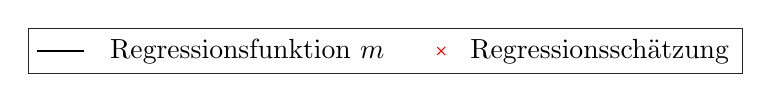
\begin{tikzpicture} 
    \begin{axis}[%
    legend columns=2,
    hide axis,
    xmin=10,
    xmax=50,
    ymin=0,
    ymax=0.4,
    legend style={draw=white!15!black,legend cell align=left,column sep=0.25cm}
    ]
    \addlegendimage{no markers,black}
    \addlegendentry{Regressionsfunktion $m \quad$};
     \addlegendimage{only marks,red,mark=x}
    \addlegendentry{Regressionsschätzung};
    \end{axis}
\end{tikzpicture}}
    \end{subfigure}
     \caption{Approximation der Regressionsfunktion $m(x) = \sin\big(\frac{\pi}{2} \cdot x^2\big)$ durch unseren Neuronale-Netze-Regressionsschätzer mit Parametern $d = 1$, $q = 2$, $R = 10^6$, $a = 3$, $N = 2$ und $M \in \{2,4,8,16\}$.}
\label{fig:subfig.a.2}
\end{figure}
\begin{figure}
    \begin{subfigure}[b]{0.5\textwidth}
    \centering
    \scalebox{0.9}{
	% This file was created by tikzplotlib v0.9.0.
\begin{tikzpicture}

\begin{axis}[
tick align=outside,
tick pos=left,
title={$N = 16$, $M = 2$},
x grid style={white!69.0196078431373!black},
xmin=-3.34207441715318, xmax=3.35388433148518,
xtick style={color=black},
y grid style={white!69.0196078431373!black},
ymin=\ymin, ymax=\ymax,
ytick style={color=black}
]
\addplot [only marks, mark=x, draw=red, fill=red, colormap/viridis]
table{%
x                      y
2.76238288932011 -0.766325584595689
-2.97867143721344 0.945972626392604
1.34016626636584 0.359459037342129
-2.34602979642214 0.796439864331818
0.262724949982951 0.11697884998794
0.761496100082008 0.826019898546403
-1.54231724537519 -0.50444448564422
2.48306325147965 -0.163379516037402
0.733875172149707 0.763973351678569
-1.60983185163084 -0.737120008728139
1.62079312559885 -0.827829522688127
-2.36695752001599 0.674869910004027
0.331351911188067 0.151868986403466
-2.43026358118505 0.239623424197933
0.485904436050117 0.341925938426166
-1.48211932367887 -0.237314469473873
0.896800847728478 0.966034627540416
1.29496171714908 0.480147772472872
0.145113687411967 0.0270108476204783
0.945128446218661 1.01035019990797
1.87976307195033 -0.611683546975155
1.84507362985819 -0.795076304770272
0.718091952323177 0.733965401288443
-0.293385227275351 0.132727176527533
-0.552300065715795 0.45208402171629
2.24848571942618 0.92528092780685
1.21759039268623 0.738609518565516
-1.89038986575959 -0.580111925801957
0.39439287977558 0.258794449086443
2.45284819380034 0.0631130541912442
-2.09586004651037 0.581982610555187
2.07310605318424 0.42472702133845
1.9212147978921 -0.423936952914823
-0.00395339221299285 0.0478843203817596
-2.77449689108578 -0.532245446691913
-2.11498496761839 0.622216094808593
2.53583216813203 -0.45431837588596
-2.73507122380883 -0.955116815815519
-0.765007401567843 0.792719597554144
0.714237808352825 0.710169847835892
-1.8183117665159 -0.873344605318397
2.88647854344178 0.598550513662334
-2.06414860173947 0.448605924099559
0.238075170967647 0.0967925788905418
0.708067946079868 0.729469699813195
-1.61406030798178 -0.823280177876845
-0.202146064743951 0.0295503219242715
-0.0539488252024247 0.0189879243978371
1.60117425795925 -0.774601047946271
0.80568451664324 0.878444379972392
-0.194699681607962 0.036321273210657
1.00165525916385 0.996116103793614
-0.27973544086681 0.114304892851678
0.154269548048458 0.029967596543592
0.951408249350171 0.989994728795778
-1.91282770827683 -0.454529854224978
1.72829730703384 -0.956682599580512
0.617192025230384 0.528943821689262
2.88199731082397 0.489716678801003
-1.66570083881295 -0.988235964670645
-0.202401155000559 0.0378205866162211
2.37385081559668 0.545429174087794
0.608600458192729 0.4976616948579
1.35575307509289 0.268707456301176
-0.517979014791838 0.418078423471025
1.10585773098792 0.923634013933351
2.67633017908538 -0.992814762837324
-1.79888360556407 -0.975392358992915
1.84419158326392 -0.779129508561444
2.81722807259938 -0.247308687468421
-2.91258760942001 0.638235599256928
-1.70874248043343 -1.01675515448634
-2.29573847812122 0.89295432601305
1.60454110644872 -0.767058329116834
-2.5127004843436 -0.364617406018911
2.99048135154545 0.509285880171684
-0.662327904724169 0.603709522380593
2.43121659559824 0.164999565026513
-1.86853437900319 -0.670944349254661
-0.354766801066255 0.21183332735161
2.06887091403722 0.393618615043543
0.571618684039537 0.444241160687973
-0.227051419851858 0.0548993056320555
0.0758984805427056 0.0217118512581678
0.443313161354085 0.338236590005564
-0.358084754486441 0.215830235438439
-1.83864625365714 -0.789129066937444
-2.31620543124488 0.825704007328304
-2.09263243577911 0.577315406796979
-2.6850542168812 -1.10356452806455
0.352058466381789 0.184846101105912
2.08632608421606 0.515960535033473
-0.845283966455336 0.922164978821915
-2.54813476418509 -0.588155479779903
-0.445653528089303 0.34512363386809
0.612047030832008 0.498187881396715
-0.447579206546175 0.352681919329291
1.86432740164422 -0.71777144900056
2.65131747712023 -0.997908502794843
2.21946463961013 0.955484680671926
1.22399698967933 0.72399418807463
-0.178206451306949 0.0214524370649
1.09618825741951 0.952268292280324
-2.91949013666082 0.710074962115307
2.89486871101226 0.650551568902872
-1.96753600902662 -0.133046626465561
2.43756237577009 0.114420336054236
1.84265940999664 -0.803387821191435
1.80083810632193 -0.867443886008529
-1.38638365328961 0.181509613264514
-1.68507716545645 -0.953145642621713
-0.427195842515467 0.318907817229158
2.09622660438393 0.565411542954988
-0.297722145169678 0.136989062006555
2.61252068404237 -0.982579994559999
-0.883924036489572 0.963191537463801
0.716352994180558 0.723410914709831
2.88419421813468 0.550743732995324
0.86077513344483 0.953927730442908
-2.72701070375638 -0.9687746217173
-0.218657454289729 0.0582721735615733
-0.991491937718017 1.00122108227183
0.193089291130048 0.102132836112914
-1.29152274832121 0.493605529607443
-2.26643261861998 0.955343109338322
1.00973393250481 0.992142368266578
1.08815852934784 0.932748403299171
2.20283579999453 0.940178924631622
-2.20571103862358 0.945232995848325
1.79172184966819 -0.94230593934244
1.96061243043077 -0.221001483239006
0.879299614506912 0.956137824195825
-1.7704671253162 -0.9906305765333
-1.43147571356497 -0.0261703171063605
-0.489019094764946 0.394462975611696
0.250794436696388 0.134090872809203
-0.135372266446698 0.00993489840682106
-0.195240647727783 0.0316465469541166
2.039044261186 0.33303048439445
2.22061419184541 0.888731273016752
1.9005237862606 -0.561321326430926
2.2668085118082 0.909945091144731
0.426052571622439 0.298993295373075
2.78421680003449 -0.455526407814202
0.639266089502806 0.569065784128471
0.623686446478088 0.530430122875644
-1.08421357755229 0.925171721659108
1.08722510470211 0.933563939428368
-2.68820586896783 -1.02586908349711
-2.19272147392835 0.890667476085183
-2.21854699456341 0.954828276166595
0.931207723348414 0.986465203989037
-1.94800444937197 -0.267086463176899
-0.953119060490716 0.999529336410753
-2.73413006500137 -0.854823962304677
-1.59759383930094 -0.710123122723663
2.78534594909577 -0.532162046993591
0.0548364150982064 0.0107398402794998
-2.09355288917141 0.526712166030853
0.138051190406785 0.026487017375763
2.66105630346648 -1.060421531295
2.194116084038 0.88615414036398
-0.647604786417679 0.563927118496397
-1.29679490415958 0.461138260089159
1.57037917615645 -0.617982010825825
-1.55709405118147 -0.568729721104781
-1.47460587205589 -0.167275764459825
-2.49548187492042 -0.237791144865769
2.18486456858416 0.956928638490545
-0.312606506278321 0.150467999138229
0.370717563659841 0.209753728278046
1.42026574616112 0.0181787242776163
1.77893320278717 -0.961324549535883
-0.314951166058117 0.157958505650292
-1.89523466294521 -0.542853788375741
1.97239710916981 -0.175369400893344
-2.81401224103046 -0.134481018740555
2.68036961764771 -0.965480585573514
0.461867078865009 0.325158744858177
2.25233243070412 0.926491076161369
0.651392621841352 0.595360983704299
-1.49004249508606 -0.322174343135326
-1.22322045902457 0.674286427889597
0.197535354189919 0.0819004224918271
2.77246927708256 -0.645517948880053
-1.89302637305893 -0.563944936249319
0.0593902688586541 -0.0377340592096357
-0.937271379378934 1.00491030062006
1.61835206974311 -0.818713736861854
1.81719891859454 -0.827064932302617
-0.4526405381867 0.364059298647535
-1.77526500003398 -0.990119656461944
-2.59746323802687 -0.990358557298789
-1.80811041347663 -0.90811047655358
-1.36559489922371 0.228479295987492
0.592733507455263 0.469988997286455
2.23850098364661 0.901108202213205
-2.23061436692708 0.939618664057149
2.74913245028938 -0.817245874810982
1.09902506312488 0.932252472880929
};
\addplot [semithick, black]
table {%
-3 1
-2.99 0.995576734820054
-2.98 0.982404791977482
-2.97 0.960687140310815
-2.96 0.930698746339696
-2.95 0.892782465918225
-2.94 0.847344438774256
-2.93 0.794849046139829
-2.92 0.735813493407208
-2.91 0.670802080787205
-2.9 0.6004202253259
-2.89 0.525308297382294
-2.88 0.446135333817727
-2.87 0.363592688736647
-2.86 0.278387680690676
-2.85 0.191237292858769
-2.84 0.102861979893671
-2.83 0.0139796319282911
-2.82 -0.0747002572851044
-2.81 -0.162482174923344
-2.8 -0.248689887164819
-2.79 -0.332671415810564
-2.78 -0.413803662790115
-2.77 -0.491496656276015
-2.76000000000001 -0.565197396549224
-2.75000000000001 -0.63439328416361
-2.74000000000001 -0.698615117310616
-2.73000000000001 -0.7574396495474
-2.72000000000001 -0.810491703188593
-2.71000000000001 -0.857445837641644
-2.70000000000001 -0.898027575760592
-2.69000000000001 -0.932014194877928
-2.68000000000001 -0.959235092527838
-2.67000000000001 -0.979571739978357
-2.66000000000001 -0.992957239530362
-2.65000000000001 -0.999375504106505
-2.64000000000001 -0.998860079935072
-2.63000000000001 -0.991492635127341
-2.62000000000001 -0.977401138650261
-2.61000000000001 -0.956757755609883
-2.60000000000001 -0.929776485888277
-2.59000000000001 -0.896710574023413
-2.58000000000001 -0.857849718795458
-2.57000000000001 -0.813517111294285
-2.56000000000001 -0.764066330303094
-2.55000000000001 -0.709878123655345
-2.54000000000001 -0.651357103821107
-2.53000000000001 -0.588928385370132
-2.52000000000001 -0.523034191158988
-2.51000000000001 -0.454130453115695
-2.50000000000001 -0.382683432365167
-2.49000000000001 -0.309166382170306
-2.48000000000001 -0.234056275775223
-2.47000000000001 -0.157830619746354
-2.46000000000001 -0.0809643718325892
-2.45000000000001 -0.00392698072389465
-2.44000000000001 0.072820436603254
-2.43000000000001 0.148827765990005
-2.42000000000001 0.223658403427451
-2.41000000000001 0.296891588141009
-2.40000000000001 0.368124552684589
-2.39000000000001 0.43697448301218
-2.38000000000001 0.503080283168017
-2.37000000000001 0.56610414086275
-2.36000000000001 0.625732891772279
-2.35000000000001 0.681679181898872
-2.34000000000001 0.733682428763456
-2.33000000000001 0.781509583546624
-2.32000000000001 0.824955697558263
-2.31000000000001 0.863844297587357
-2.30000000000001 0.898027575760569
-2.29000000000002 0.927386400518292
-2.28000000000002 0.951830156198068
-2.27000000000002 0.971296419496836
-2.26000000000002 0.985750481765479
-2.25000000000002 0.995184726672186
-2.24000000000002 0.999617873256875
-2.23000000000002 0.999094094789406
-2.22000000000002 0.993682024142277
-2.21000000000002 0.983473656597255
-2.20000000000002 0.96858316112866
-2.19000000000002 0.949145611247931
-2.18000000000002 0.925315646459183
-2.17000000000002 0.897266075268519
-2.16000000000002 0.865186430515806
-2.15000000000002 0.829281487561826
-2.14000000000002 0.789769755571343
-2.13000000000002 0.746881951789148
-2.12000000000002 0.700859468316991
-2.11000000000002 0.651952840469899
-2.10000000000002 0.600420225325985
-2.09000000000002 0.546525898589853
-2.08000000000002 0.490538777371198
-2.07000000000002 0.432730975942088
-2.06000000000002 0.373376400983612
-2.05000000000002 0.31274939226965
-2.04000000000002 0.251123414166708
-2.03000000000002 0.188769802758421
-2.02000000000002 0.125956572835066
-2.01000000000002 0.062947288426061
-2.00000000000002 1.33870012014889e-13
-1.99000000000002 -0.062633749083271
-1.98000000000002 -0.124709844813965
-1.97000000000002 -0.185992451913749
-1.96000000000002 -0.246254789302508
-1.95000000000002 -0.305279831055913
-1.94000000000002 -0.3628609327075
-1.93000000000002 -0.418802383167873
-1.92000000000002 -0.472919882928091
-1.91000000000002 -0.525040949582032
-1.90000000000002 -0.575005252043164
-1.89000000000002 -0.622664875144035
-1.88000000000002 -0.667884516592001
-1.87000000000002 -0.710541618511978
-1.86000000000002 -0.750526436036607
-1.85000000000002 -0.787742045606543
-1.84000000000002 -0.822104295818981
-1.83000000000002 -0.85354170381174
-1.82000000000003 -0.881995300293982
-1.81000000000003 -0.907418426433774
-1.80000000000003 -0.929776485888198
-1.79000000000003 -0.949046655314642
-1.78000000000003 -0.965217556733346
-1.77000000000003 -0.978288895122437
-1.76000000000003 -0.988271064618766
-1.75000000000003 -0.995184726672183
-1.74000000000003 -0.99906036345861
-1.73000000000003 -0.999937809799883
-1.72000000000003 -0.997865766766904
-1.71000000000003 -0.992901300058717
-1.70000000000003 -0.985109326154799
-1.69000000000003 -0.974562089132473
-1.68000000000003 -0.961338630927184
-1.67000000000003 -0.945524257691589
-1.66000000000003 -0.92721000478115
-1.65000000000003 -0.906492102760418
-1.64000000000003 -0.883471446686396
-1.63000000000003 -0.858253070784441
-1.62000000000003 -0.830945630488965
-1.61000000000003 -0.801660893676759
-1.60000000000003 -0.770513242775885
-1.59000000000003 -0.737619189288572
-1.58000000000003 -0.703096902123257
-1.57000000000003 -0.667065750989361
-1.56000000000003 -0.629645865969377
-1.55000000000003 -0.590957714246878
-1.54000000000003 -0.5511216948366
-1.53000000000003 -0.510257752034371
-1.52000000000003 -0.468485008180726
-1.51000000000003 -0.425921416212823
-1.50000000000003 -0.382683432365229
-1.49000000000003 -0.338885709271396
-1.48000000000003 -0.29464080961443
-1.47000000000003 -0.250058940378286
-1.46000000000003 -0.205247707658841
-1.45000000000003 -0.16031189190854
-1.44000000000003 -0.115353243408457
-1.43000000000003 -0.0704702976877775
-1.42000000000003 -0.0257582105426693
-1.41000000000003 0.018691387755514
-1.40000000000003 0.0627905195291638
-1.39000000000003 0.106454968557562
-1.38000000000003 0.149604371296494
-1.37000000000003 0.192162291056312
-1.36000000000003 0.234056275774993
-1.35000000000004 0.275217900052248
-1.34000000000004 0.315582792135412
-1.33000000000004 0.355090646567928
-1.32000000000004 0.393685223226887
-1.31000000000004 0.431314333487567
-1.30000000000004 0.467929814260443
-1.29000000000004 0.503487490649953
-1.28000000000004 0.537947127984647
-1.27000000000004 0.571272373965398
-1.26000000000004 0.603430691672474
-1.25000000000004 0.634393284163532
-1.24000000000004 0.664135011383361
-1.23000000000004 0.692634300092632
-1.22000000000004 0.719873047507249
-1.21000000000004 0.745836519322339
-1.20000000000004 0.770513242775697
-1.19000000000004 0.79389489538482
-1.18000000000004 0.815976189969678
-1.17000000000004 0.836754756550324
-1.16000000000004 0.856231021684473
-1.15000000000004 0.87440808578545
-1.14000000000004 0.891291598935659
-1.13000000000004 0.906889635684947
-1.12000000000004 0.921212569297285
-1.11000000000004 0.93427294588298
-1.10000000000004 0.9460853588275
-1.09000000000004 0.956666323901834
-1.08000000000004 0.966034155413461
-1.07000000000004 0.974208843731348
-1.06000000000004 0.981211934493193
-1.05000000000004 0.987066409778344
-1.04000000000004 0.991796571505593
-1.03000000000004 0.995427927291427
-1.02000000000004 0.997987078981312
-1.01000000000004 0.999501614044331
-1.00000000000004 1
-0.990000000000043 0.999511482025296
-0.980000000000043 0.998065983870084
-0.970000000000043 0.995694012190007
-0.960000000000043 0.992426564387702
-0.950000000000044 0.988295040035889
-0.940000000000044 0.983331155939389
-0.930000000000044 0.977566864877576
-0.920000000000044 0.971034278054095
-0.910000000000045 0.963765591266851
-0.900000000000045 0.955793014798367
-0.890000000000045 0.94714870701456
-0.880000000000045 0.937864711648732
-0.870000000000045 0.927972898737259
-0.860000000000046 0.917504909163832
-0.850000000000046 0.906492102760406
-0.840000000000046 0.894965509904969
-0.830000000000046 0.882955786549018
-0.820000000000046 0.870493172601118
-0.810000000000047 0.857607453587072
-0.800000000000047 0.844327925502078
-0.790000000000047 0.830683362765738
-0.780000000000047 0.816701989186866
-0.770000000000048 0.802411451841723
-0.760000000000048 0.787838797766522
-0.750000000000048 0.773010453362809
-0.740000000000048 0.757952206412552
-0.730000000000048 0.742689190598499
-0.720000000000049 0.727245872424471
-0.710000000000049 0.711646040429847
-0.700000000000049 0.695912796592392
-0.690000000000049 0.68006854981388
-0.680000000000049 0.664135011383549
-0.67000000000005 0.648133192315342
-0.66000000000005 0.632083402456062
-0.65000000000005 0.61600525126299
-0.64000000000005 0.599917650151169
-0.630000000000051 0.583838816312412
-0.620000000000051 0.567786277910133
-0.610000000000051 0.551776880556293
-0.600000000000051 0.535826794979078
-0.590000000000051 0.519951525792427
-0.580000000000052 0.504165921281037
-0.570000000000052 0.488484184117171
-0.560000000000052 0.472919882928293
-0.550000000000052 0.457485964637341
-0.540000000000052 0.442194767500267
-0.530000000000053 0.427058034768333
-0.520000000000053 0.4120869289055
-0.510000000000053 0.397292046294142
-0.500000000000053 0.382683432365167
-0.490000000000054 0.368270597091477
-0.480000000000054 0.354062530786545
-0.470000000000054 0.340067720152659
-0.460000000000054 0.326294164526146
-0.450000000000054 0.312749392269599
-0.440000000000055 0.299440477263786
-0.430000000000055 0.286374055454505
-0.420000000000055 0.273556341412193
-0.410000000000055 0.260993144864562
-0.400000000000055 0.248689887164922
-0.390000000000056 0.23665161766118
-0.380000000000056 0.22488302993274
-0.370000000000056 0.213388477864702
-0.360000000000056 0.202171991530836
-0.350000000000056 0.191237292858801
-0.340000000000057 0.180587811053027
-0.330000000000057 0.170226697752469
-0.320000000000057 0.160156841902239
-0.310000000000057 0.150380884319751
-0.300000000000058 0.140901231937636
-0.290000000000058 0.131720071707145
-0.280000000000058 0.122839384147215
-0.270000000000058 0.114260956525697
-0.260000000000058 0.105986395660502
-0.250000000000059 0.0980171403296064
-0.240000000000059 0.0903544732799798
-0.230000000000059 0.0829995328265039
-0.220000000000059 0.0759533240329385
-0.210000000000059 0.0692167294678623
-0.20000000000006 0.0627905195293508
-0.19000000000006 0.0566753623329036
-0.18000000000006 0.0508718331578319
-0.17000000000006 0.0453804234479493
-0.160000000000061 0.0402015493629836
-0.150000000000061 0.0353355598776498
-0.140000000000061 0.0307827444257893
-0.130000000000061 0.0265433400874004
-0.120000000000061 0.0226175383167529
-0.110000000000062 0.019005491210107
-0.100000000000062 0.0157073173118401
-0.090000000000062 0.012723106958029
-0.0800000000000622 0.0100529271567463
-0.0700000000000625 0.00769682600450373
-0.0600000000000627 0.00565483663842069
-0.0500000000000629 0.00392698072381588
-0.0400000000000631 0.00251327147701166
-0.0300000000000633 0.00141371622321359
-0.0200000000000635 0.000628318489380248
-0.0100000000000637 0.000157079632035528
-6.3948846218409e-14 6.42370078682459e-27
0.00999999999993584 0.00015707963203151
0.0199999999999356 0.000628318489372212
0.0299999999999354 0.00141371622320154
0.0399999999999352 0.00251327147699558
0.049999999999935 0.00392698072379579
0.0599999999999348 0.00565483663839659
0.0699999999999346 0.00769682600447561
0.0799999999999343 0.0100529271567142
0.0899999999999341 0.0127231069579928
0.0999999999999339 0.0157073173117999
0.109999999999934 0.0190054912100628
0.119999999999933 0.0226175383167047
0.129999999999933 0.0265433400873482
0.139999999999933 0.0307827444257331
0.149999999999933 0.0353355598775896
0.159999999999933 0.0402015493629194
0.169999999999932 0.045380423447881
0.179999999999932 0.0508718331577597
0.189999999999932 0.0566753623328273
0.199999999999932 0.0627905195292706
0.209999999999932 0.0692167294677781
0.219999999999931 0.0759533240328503
0.229999999999931 0.0829995328264118
0.239999999999931 0.0903544732798837
0.249999999999931 0.0980171403295065
0.259999999999931 0.105986395660398
0.26999999999993 0.114260956525589
0.27999999999993 0.122839384147103
0.28999999999993 0.131720071707029
0.29999999999993 0.140901231937517
0.309999999999929 0.150380884319628
0.319999999999929 0.160156841902112
0.329999999999929 0.170226697752338
0.339999999999929 0.180587811052893
0.349999999999929 0.191237292858663
0.359999999999928 0.202171991530694
0.369999999999928 0.213388477864557
0.379999999999928 0.224883029932591
0.389999999999928 0.236651617661028
0.399999999999928 0.248689887164767
0.409999999999927 0.260993144864403
0.419999999999927 0.273556341412031
0.429999999999927 0.28637405545434
0.439999999999927 0.299440477263618
0.449999999999926 0.312749392269427
0.459999999999926 0.326294164525971
0.469999999999926 0.340067720152481
0.479999999999926 0.354062530786364
0.489999999999926 0.368270597091294
0.499999999999925 0.382683432364981
0.509999999999925 0.397292046293954
0.519999999999925 0.412086928905309
0.529999999999925 0.42705803476814
0.539999999999925 0.442194767500072
0.549999999999924 0.457485964637144
0.559999999999924 0.472919882928095
0.569999999999924 0.488484184116971
0.579999999999924 0.504165921280836
0.589999999999923 0.519951525792225
0.599999999999923 0.535826794978874
0.609999999999923 0.551776880556088
0.619999999999923 0.567786277909928
0.629999999999923 0.583838816312206
0.639999999999922 0.599917650150963
0.649999999999922 0.616005251262785
0.659999999999922 0.632083402455857
0.669999999999922 0.648133192315137
0.679999999999922 0.664135011383345
0.689999999999921 0.680068549813677
0.699999999999921 0.69591279659219
0.709999999999921 0.711646040429646
0.719999999999921 0.727245872424273
0.72999999999992 0.742689190598303
0.73999999999992 0.757952206412358
0.74999999999992 0.773010453362617
0.75999999999992 0.787838797766334
0.76999999999992 0.802411451841539
0.779999999999919 0.816701989186685
0.789999999999919 0.830683362765561
0.799999999999919 0.844327925501906
0.809999999999919 0.857607453586905
0.819999999999919 0.870493172600956
0.829999999999918 0.882955786548861
0.839999999999918 0.894965509904818
0.849999999999918 0.906492102760262
0.859999999999918 0.917504909163694
0.869999999999918 0.927972898737128
0.879999999999917 0.93786471164861
0.889999999999917 0.947148707014445
0.899999999999917 0.955793014798261
0.909999999999917 0.963765591266753
0.919999999999916 0.971034278054007
0.929999999999916 0.977566864877497
0.939999999999916 0.98333115593932
0.949999999999916 0.988295040035831
0.959999999999916 0.992426564387655
0.969999999999915 0.995694012189971
0.979999999999915 0.99806598387006
0.989999999999915 0.999511482025283
0.999999999999915 1
1.00999999999991 0.999501614044344
1.01999999999991 0.997987078981338
1.02999999999991 0.995427927291467
1.03999999999991 0.991796571505646
1.04999999999991 0.987066409778411
1.05999999999991 0.981211934493276
1.06999999999991 0.974208843731445
1.07999999999991 0.966034155413573
1.08999999999991 0.956666323901962
1.09999999999991 0.946085358827643
1.10999999999991 0.934272945883139
1.11999999999991 0.92121256929746
1.12999999999991 0.906889635685138
1.13999999999991 0.891291598935866
1.14999999999991 0.874408085785674
1.15999999999991 0.856231021684713
1.16999999999991 0.836754756550582
1.17999999999991 0.815976189969952
1.18999999999991 0.793894895385111
1.19999999999991 0.770513242776004
1.20999999999991 0.745836519322663
1.21999999999991 0.719873047507589
1.22999999999991 0.692634300092988
1.23999999999991 0.664135011383733
1.24999999999991 0.63439328416392
1.25999999999991 0.603430691672878
1.26999999999991 0.571272373965817
1.27999999999991 0.537947127985081
1.28999999999991 0.503487490650401
1.29999999999991 0.467929814260904
1.30999999999991 0.431314333488042
1.31999999999991 0.393685223227375
1.32999999999991 0.355090646568427
1.33999999999991 0.315582792135923
1.34999999999991 0.27521790005277
1.35999999999991 0.234056275775525
1.36999999999991 0.192162291056853
1.37999999999991 0.149604371297043
1.38999999999991 0.106454968558117
1.39999999999991 0.0627905195297253
1.40999999999991 0.0186913877560805
1.41999999999991 -0.0257582105420993
1.42999999999991 -0.0704702976872039
1.43999999999991 -0.115353243407883
1.44999999999991 -0.160311891907964
1.4599999999999 -0.205247707658268
1.4699999999999 -0.250058940377715
1.4799999999999 -0.294640809613862
1.4899999999999 -0.338885709270833
1.4999999999999 -0.382683432364672
1.5099999999999 -0.425921416212274
1.5199999999999 -0.468485008180186
1.5299999999999 -0.510257752033843
1.5399999999999 -0.551121694836084
1.5499999999999 -0.590957714246376
1.5599999999999 -0.62964586596889
1.5699999999999 -0.667065750988891
1.5799999999999 -0.703096902122806
1.5899999999999 -0.73761918928814
1.5999999999999 -0.770513242775475
1.6099999999999 -0.801660893676373
1.6199999999999 -0.830945630488602
1.6299999999999 -0.858253070784105
1.6399999999999 -0.883471446686087
1.6499999999999 -0.906492102760138
1.6599999999999 -0.9272100047809
1.6699999999999 -0.945524257691371
1.6799999999999 -0.961338630926998
1.6899999999999 -0.974562089132321
1.6999999999999 -0.985109326154682
1.7099999999999 -0.992901300058635
1.7199999999999 -0.997865766766859
1.7299999999999 -0.999937809799876
1.7399999999999 -0.99906036345864
1.7499999999999 -0.995184726672251
1.7599999999999 -0.988271064618874
1.7699999999999 -0.978288895122584
1.7799999999999 -0.965217556733533
1.7899999999999 -0.949046655314868
1.7999999999999 -0.929776485888465
1.8099999999999 -0.90741842643408
1.8199999999999 -0.881995300294327
1.8299999999999 -0.853541703812123
1.8399999999999 -0.822104295819402
1.8499999999999 -0.787742045607001
1.8599999999999 -0.750526436037101
1.8699999999999 -0.710541618512508
1.8799999999999 -0.667884516592564
1.8899999999999 -0.622664875144629
1.8999999999999 -0.575005252043788
1.9099999999999 -0.525040949582685
1.9199999999999 -0.47291988292877
1.92999999999989 -0.418802383168577
1.93999999999989 -0.362860932708227
1.94999999999989 -0.305279831056659
1.95999999999989 -0.246254789303272
1.96999999999989 -0.185992451914526
1.97999999999989 -0.124709844814754
1.98999999999989 -0.0626337490840697
1.99999999999989 -6.69931457813724e-13
2.00999999999989 0.0629472884252544
2.01999999999989 0.12595657283426
2.02999999999989 0.18876980275762
2.03999999999989 0.251123414165916
2.04999999999989 0.312749392268867
2.05999999999989 0.373376400982844
2.06999999999989 0.432730975941339
2.07999999999989 0.490538777370471
2.08999999999989 0.54652589858915
2.09999999999989 0.600420225325311
2.10999999999989 0.651952840469257
2.11999999999989 0.700859468316383
2.12999999999989 0.746881951788579
2.13999999999989 0.789769755570817
2.14999999999989 0.829281487561343
2.15999999999989 0.865186430515371
2.16999999999989 0.897266075268134
2.17999999999989 0.925315646458851
2.18999999999989 0.949145611247653
2.19999999999989 0.968583161128441
2.20999999999989 0.983473656597094
2.21999999999989 0.993682024142177
2.22999999999989 0.999094094789368
2.23999999999989 0.9996178732569
2.24999999999989 0.995184726672274
2.25999999999989 0.985750481765632
2.26999999999989 0.971296419497053
2.27999999999989 0.951830156198348
2.28999999999989 0.927386400518636
2.29999999999989 0.898027575760974
2.30999999999989 0.863844297587825
2.31999999999989 0.82495569755879
2.32999999999989 0.781509583547208
2.33999999999989 0.733682428764095
2.34999999999989 0.681679181899562
2.35999999999989 0.625732891773019
2.36999999999989 0.566104140863535
2.37999999999989 0.503080283168843
2.38999999999989 0.436974483013044
2.39999999999988 0.368124552685486
2.40999999999988 0.296891588141934
2.41999999999988 0.2236584034284
2.42999999999988 0.148827765990971
2.43999999999988 0.072820436604232
2.44999999999988 -0.00392698072291233
2.45999999999988 -0.0809643718316048
2.46999999999988 -0.157830619745374
2.47999999999988 -0.234056275774253
2.48999999999988 -0.309166382169355
2.49999999999988 -0.382683432364238
2.50999999999988 -0.454130453114798
2.51999999999988 -0.523034191158123
2.52999999999988 -0.58892838536931
2.53999999999988 -0.651357103820333
2.54999999999988 -0.709878123654623
2.55999999999988 -0.764066330302429
2.56999999999988 -0.813517111293685
2.57999999999988 -0.857849718794925
2.58999999999988 -0.896710574022952
2.59999999999988 -0.929776485887892
2.60999999999988 -0.956757755609577
2.61999999999988 -0.977401138650039
2.62999999999988 -0.991492635127203
2.63999999999988 -0.998860079935021
2.64999999999988 -0.999375504106543
2.65999999999988 -0.992957239530489
2.66999999999988 -0.979571739978573
2.67999999999988 -0.959235092528142
2.68999999999988 -0.93201419487832
2.69999999999988 -0.898027575761069
2.70999999999988 -0.857445837642205
2.71999999999988 -0.810491703189233
2.72999999999988 -0.757439649548115
2.73999999999988 -0.698615117311402
2.74999999999988 -0.634393284164464
2.75999999999988 -0.565197396550139
2.76999999999988 -0.491496656276984
2.77999999999988 -0.413803662791132
2.78999999999988 -0.332671415811622
2.79999999999988 -0.248689887165909
2.80999999999988 -0.162482174924459
2.81999999999988 -0.0747002572862345
2.82999999999988 0.0139796319271562
2.83999999999988 0.102861979892536
2.84999999999988 0.191237292857646
2.85999999999988 0.278387680689572
2.86999999999987 0.36359268873557
2.87999999999987 0.44613533381669
2.88999999999987 0.525308297381304
2.89999999999987 0.600420225324967
2.90999999999987 0.670802080786339
2.91999999999987 0.735813493406414
2.92999999999987 0.794849046139114
2.93999999999987 0.847344438773628
2.94999999999987 0.892782465917691
2.95999999999987 0.930698746339261
2.96999999999987 0.960687140310484
2.97999999999987 0.982404791977258
2.98999999999987 0.995576734819941
};
\end{axis}

\end{tikzpicture}
}
        \label{fig:subfig3n16m2}
    \end{subfigure}
    \begin{subfigure}[b]{0.5\textwidth}
    \centering
     \scalebox{0.9}{
           % This file was created by tikzplotlib v0.9.0.
\begin{tikzpicture}

\begin{axis}[
tick align=outside,
tick pos=left,
title={$N = 16$, $M = 4$},
x grid style={white!69.0196078431373!black},
xmin=-3.34207441715318, xmax=3.35388433148518,
xtick style={color=black},
y grid style={white!69.0196078431373!black},
ymin=\ymin, ymax=\ymax,
ytick style={color=black}
]
\addplot [only marks, mark=x, draw=red, fill=red, colormap/viridis]
table{%
x                      y
2.76238288932011 -0.519271516963569
-2.97867143721344 0.627718402332759
1.34016626636584 0.347148648797896
-2.34602979642214 0.715293342815513
0.262724949982951 0.126168537021242
0.761496100082008 0.794628751103097
-1.54231724537519 -0.507219104537765
2.48306325147965 -0.217663447371128
0.733875172149707 0.749471083566891
-1.60983185163084 -0.803246565499583
1.62079312559885 -0.824378652668729
-2.36695752001599 0.540436504325082
0.331351911188067 0.184474726693494
-2.43026358118505 0.339081003949203
0.485904436050117 0.361603201298078
-1.48211932367887 -0.278258837336831
0.896800847728478 0.954828455595081
1.29496171714908 0.492879422526084
0.145113687411967 0.0418804582369513
0.945128446218661 0.980948725004782
1.87976307195033 -0.661988223527526
1.84507362985819 -0.784597790814253
0.718091952323177 0.735082557629091
-0.293385227275351 0.117551274496956
-0.552300065715795 0.445961980349349
2.24848571942618 1.00254618361199
1.21759039268623 0.726949692325361
-1.89038986575959 -0.561979730458363
0.39439287977558 0.245033793108948
2.45284819380034 -0.0217896751452117
-2.09586004651037 0.615618577611782
2.07310605318424 0.427816570346922
1.9212147978921 -0.465006032346679
-0.00395339221299285 -0.00355657961998001
-2.77449689108578 -0.812840665285465
-2.11498496761839 0.576789701806356
2.53583216813203 -0.582433411051381
-2.73507122380883 -0.712165729553937
-0.765007401567843 0.789049205862463
0.714237808352825 0.719160887534074
-1.8183117665159 -0.81854722466509
2.88647854344178 0.508582045344982
-2.06414860173947 0.520015192624974
0.238075170967647 0.123189490643356
0.708067946079868 0.707056945309492
-1.61406030798178 -0.868553296908103
-0.202146064743951 0.0483600187430168
-0.0539488252024247 0.0233580496851449
1.60117425795925 -0.754760924260003
0.80568451664324 0.877004902395915
-0.194699681607962 0.0527334962773332
1.00165525916385 0.995915799199225
-0.27973544086681 0.104541382073973
0.154269548048458 0.0266021544620167
0.951408249350171 0.991227470132248
-1.91282770827683 -0.408507353482738
1.72829730703384 -0.979865481201272
0.617192025230384 0.54818751011403
2.88199731082397 0.465367639768135
-1.66570083881295 -1.02500820101851
-0.202401155000559 0.0580927512205558
2.37385081559668 0.505025562206135
0.608600458192729 0.529879830385007
1.35575307509289 0.250799303791182
-0.517979014791838 0.368021150358684
1.10585773098792 0.958073933454405
2.67633017908538 -0.966938827261329
-1.79888360556407 -0.973380045023673
1.84419158326392 -0.802852494808031
2.81722807259938 -0.0802092320985084
-2.91258760942001 0.818280949630541
-1.70874248043343 -1.05008528110908
-2.29573847812122 0.919301784531309
1.60454110644872 -0.765834257045759
-2.5127004843436 -0.333221300883163
2.99048135154545 0.941100371355591
-0.662327904724169 0.6426660679032
2.43121659559824 0.132413944148037
-1.86853437900319 -0.660256946525661
-0.354766801066255 0.195501071079521
2.06887091403722 0.399474873542834
0.571618684039537 0.475554232522144
-0.227051419851858 0.0775578627420259
0.0758984805427056 -0.0102733053592664
0.443313161354085 0.313832173367835
-0.358084754486441 0.207626243638239
-1.83864625365714 -0.707476232905346
-2.31620543124488 0.680566860111479
-2.09263243577911 0.547658905512773
-2.6850542168812 -1.16120414700005
0.352058466381789 0.207033983904641
2.08632608421606 0.494122694881404
-0.845283966455336 0.912052518146741
-2.54813476418509 -0.632519642035432
-0.445653528089303 0.300263016728058
0.612047030832008 0.532713028085415
-0.447579206546175 0.310455193249083
1.86432740164422 -0.730265516287387
2.65131747712023 -0.979538195743698
2.21946463961013 1.00152114488393
1.22399698967933 0.718098767971379
-0.178206451306949 0.048133287139278
1.09618825741951 0.962357515314418
-2.91949013666082 0.442131420316021
2.89486871101226 0.594071449923684
-1.96753600902662 -0.12458758303484
2.43756237577009 0.0571182560448527
1.84265940999664 -0.794058273353083
1.80083810632193 -0.900592382404695
-1.38638365328961 0.161849660397942
-1.68507716545645 -0.930981285037446
-0.427195842515467 0.283075308896927
2.09622660438393 0.549114475412099
-0.297722145169678 0.125089082151998
2.61252068404237 -0.95100256196209
-0.883924036489572 0.932593222327429
0.716352994180558 0.704989704007166
2.88419421813468 0.449563487306245
0.86077513344483 0.928761202440283
-2.72701070375638 -0.847985020489822
-0.218657454289729 0.082493396633992
-0.991491937718017 1.00607534588063
0.193089291130048 0.0738503944306138
-1.29152274832121 0.494306202809488
-2.26643261861998 0.755966518048505
1.00973393250481 0.998212832033248
1.08815852934784 0.975001878002125
2.20283579999453 0.986063627686408
-2.20571103862358 0.842798619648536
1.79172184966819 -0.919934343815097
1.96061243043077 -0.229959050720918
0.879299614506912 0.951187806542893
-1.7704671253162 -0.987363554054566
-1.43147571356497 -0.0689129309167798
-0.489019094764946 0.35517924324034
0.250794436696388 0.109938371058934
-0.135372266446698 0.0356745490523402
-0.195240647727783 0.0445363501225547
2.039044261186 0.233676813088956
2.22061419184541 1.00488313685484
1.9005237862606 -0.586720281812891
2.2668085118082 0.957763620746453
0.426052571622439 0.275379868935167
2.78421680003449 -0.396192369844326
0.639266089502806 0.585256181110867
0.623686446478088 0.557037530021373
-1.08421357755229 0.955893247865414
1.08722510470211 0.964549176713506
-2.68820586896783 -0.760398040702336
-2.19272147392835 0.846824630394737
-2.21854699456341 0.920208880433863
0.931207723348414 0.982701926011991
-1.94800444937197 -0.175106464359253
-0.953119060490716 0.979072331333819
-2.73413006500137 -1.01210852715816
-1.59759383930094 -0.698265182223175
2.78534594909577 -0.359018520524818
0.0548364150982064 0.00567438897326111
-2.09355288917141 0.520749545210161
0.138051190406785 0.0231764622551443
2.66105630346648 -0.99083113717891
2.194116084038 0.955349575072848
-0.647604786417679 0.59949755680119
-1.29679490415958 0.484080382077781
1.57037917615645 -0.68701075461458
-1.55709405118147 -0.561540870757727
-1.47460587205589 -0.194735885571855
-2.49548187492042 -0.155593831363912
2.18486456858416 0.936257538347677
-0.312606506278321 0.130052560811128
0.370717563659841 0.215992724355017
1.42026574616112 -0.0134772947367084
1.77893320278717 -0.948594917074905
-0.314951166058117 0.132475254869048
-1.89523466294521 -0.518494539417829
1.97239710916981 -0.180961544080235
-2.81401224103046 -0.288015559206678
2.68036961764771 -0.948064646510748
0.461867078865009 0.327011032002142
2.25233243070412 0.991778078012125
0.651392621841352 0.600489152403728
-1.49004249508606 -0.388267052271327
-1.22322045902457 0.67644645054974
0.197535354189919 0.0735875626609471
2.77246927708256 -0.495058103894625
-1.89302637305893 -0.539427016076772
0.0593902688586541 -0.00258565955697071
-0.937271379378934 0.984958724650048
1.61835206974311 -0.797995985236732
1.81719891859454 -0.862479895181206
-0.4526405381867 0.330366294940942
-1.77526500003398 -1.01483785584784
-2.59746323802687 -0.947848279775752
-1.80811041347663 -0.875937215232482
-1.36559489922371 0.210179995089497
0.592733507455263 0.496412450423355
2.23850098364661 1.0047969690488
-2.23061436692708 0.895314461347219
2.74913245028938 -0.603239184671184
1.09902506312488 0.956980048023673
};
\addplot [semithick, black]
table {%
-3 1
-2.99 0.995576734820054
-2.98 0.982404791977482
-2.97 0.960687140310815
-2.96 0.930698746339696
-2.95 0.892782465918225
-2.94 0.847344438774256
-2.93 0.794849046139829
-2.92 0.735813493407208
-2.91 0.670802080787205
-2.9 0.6004202253259
-2.89 0.525308297382294
-2.88 0.446135333817727
-2.87 0.363592688736647
-2.86 0.278387680690676
-2.85 0.191237292858769
-2.84 0.102861979893671
-2.83 0.0139796319282911
-2.82 -0.0747002572851044
-2.81 -0.162482174923344
-2.8 -0.248689887164819
-2.79 -0.332671415810564
-2.78 -0.413803662790115
-2.77 -0.491496656276015
-2.76000000000001 -0.565197396549224
-2.75000000000001 -0.63439328416361
-2.74000000000001 -0.698615117310616
-2.73000000000001 -0.7574396495474
-2.72000000000001 -0.810491703188593
-2.71000000000001 -0.857445837641644
-2.70000000000001 -0.898027575760592
-2.69000000000001 -0.932014194877928
-2.68000000000001 -0.959235092527838
-2.67000000000001 -0.979571739978357
-2.66000000000001 -0.992957239530362
-2.65000000000001 -0.999375504106505
-2.64000000000001 -0.998860079935072
-2.63000000000001 -0.991492635127341
-2.62000000000001 -0.977401138650261
-2.61000000000001 -0.956757755609883
-2.60000000000001 -0.929776485888277
-2.59000000000001 -0.896710574023413
-2.58000000000001 -0.857849718795458
-2.57000000000001 -0.813517111294285
-2.56000000000001 -0.764066330303094
-2.55000000000001 -0.709878123655345
-2.54000000000001 -0.651357103821107
-2.53000000000001 -0.588928385370132
-2.52000000000001 -0.523034191158988
-2.51000000000001 -0.454130453115695
-2.50000000000001 -0.382683432365167
-2.49000000000001 -0.309166382170306
-2.48000000000001 -0.234056275775223
-2.47000000000001 -0.157830619746354
-2.46000000000001 -0.0809643718325892
-2.45000000000001 -0.00392698072389465
-2.44000000000001 0.072820436603254
-2.43000000000001 0.148827765990005
-2.42000000000001 0.223658403427451
-2.41000000000001 0.296891588141009
-2.40000000000001 0.368124552684589
-2.39000000000001 0.43697448301218
-2.38000000000001 0.503080283168017
-2.37000000000001 0.56610414086275
-2.36000000000001 0.625732891772279
-2.35000000000001 0.681679181898872
-2.34000000000001 0.733682428763456
-2.33000000000001 0.781509583546624
-2.32000000000001 0.824955697558263
-2.31000000000001 0.863844297587357
-2.30000000000001 0.898027575760569
-2.29000000000002 0.927386400518292
-2.28000000000002 0.951830156198068
-2.27000000000002 0.971296419496836
-2.26000000000002 0.985750481765479
-2.25000000000002 0.995184726672186
-2.24000000000002 0.999617873256875
-2.23000000000002 0.999094094789406
-2.22000000000002 0.993682024142277
-2.21000000000002 0.983473656597255
-2.20000000000002 0.96858316112866
-2.19000000000002 0.949145611247931
-2.18000000000002 0.925315646459183
-2.17000000000002 0.897266075268519
-2.16000000000002 0.865186430515806
-2.15000000000002 0.829281487561826
-2.14000000000002 0.789769755571343
-2.13000000000002 0.746881951789148
-2.12000000000002 0.700859468316991
-2.11000000000002 0.651952840469899
-2.10000000000002 0.600420225325985
-2.09000000000002 0.546525898589853
-2.08000000000002 0.490538777371198
-2.07000000000002 0.432730975942088
-2.06000000000002 0.373376400983612
-2.05000000000002 0.31274939226965
-2.04000000000002 0.251123414166708
-2.03000000000002 0.188769802758421
-2.02000000000002 0.125956572835066
-2.01000000000002 0.062947288426061
-2.00000000000002 1.33870012014889e-13
-1.99000000000002 -0.062633749083271
-1.98000000000002 -0.124709844813965
-1.97000000000002 -0.185992451913749
-1.96000000000002 -0.246254789302508
-1.95000000000002 -0.305279831055913
-1.94000000000002 -0.3628609327075
-1.93000000000002 -0.418802383167873
-1.92000000000002 -0.472919882928091
-1.91000000000002 -0.525040949582032
-1.90000000000002 -0.575005252043164
-1.89000000000002 -0.622664875144035
-1.88000000000002 -0.667884516592001
-1.87000000000002 -0.710541618511978
-1.86000000000002 -0.750526436036607
-1.85000000000002 -0.787742045606543
-1.84000000000002 -0.822104295818981
-1.83000000000002 -0.85354170381174
-1.82000000000003 -0.881995300293982
-1.81000000000003 -0.907418426433774
-1.80000000000003 -0.929776485888198
-1.79000000000003 -0.949046655314642
-1.78000000000003 -0.965217556733346
-1.77000000000003 -0.978288895122437
-1.76000000000003 -0.988271064618766
-1.75000000000003 -0.995184726672183
-1.74000000000003 -0.99906036345861
-1.73000000000003 -0.999937809799883
-1.72000000000003 -0.997865766766904
-1.71000000000003 -0.992901300058717
-1.70000000000003 -0.985109326154799
-1.69000000000003 -0.974562089132473
-1.68000000000003 -0.961338630927184
-1.67000000000003 -0.945524257691589
-1.66000000000003 -0.92721000478115
-1.65000000000003 -0.906492102760418
-1.64000000000003 -0.883471446686396
-1.63000000000003 -0.858253070784441
-1.62000000000003 -0.830945630488965
-1.61000000000003 -0.801660893676759
-1.60000000000003 -0.770513242775885
-1.59000000000003 -0.737619189288572
-1.58000000000003 -0.703096902123257
-1.57000000000003 -0.667065750989361
-1.56000000000003 -0.629645865969377
-1.55000000000003 -0.590957714246878
-1.54000000000003 -0.5511216948366
-1.53000000000003 -0.510257752034371
-1.52000000000003 -0.468485008180726
-1.51000000000003 -0.425921416212823
-1.50000000000003 -0.382683432365229
-1.49000000000003 -0.338885709271396
-1.48000000000003 -0.29464080961443
-1.47000000000003 -0.250058940378286
-1.46000000000003 -0.205247707658841
-1.45000000000003 -0.16031189190854
-1.44000000000003 -0.115353243408457
-1.43000000000003 -0.0704702976877775
-1.42000000000003 -0.0257582105426693
-1.41000000000003 0.018691387755514
-1.40000000000003 0.0627905195291638
-1.39000000000003 0.106454968557562
-1.38000000000003 0.149604371296494
-1.37000000000003 0.192162291056312
-1.36000000000003 0.234056275774993
-1.35000000000004 0.275217900052248
-1.34000000000004 0.315582792135412
-1.33000000000004 0.355090646567928
-1.32000000000004 0.393685223226887
-1.31000000000004 0.431314333487567
-1.30000000000004 0.467929814260443
-1.29000000000004 0.503487490649953
-1.28000000000004 0.537947127984647
-1.27000000000004 0.571272373965398
-1.26000000000004 0.603430691672474
-1.25000000000004 0.634393284163532
-1.24000000000004 0.664135011383361
-1.23000000000004 0.692634300092632
-1.22000000000004 0.719873047507249
-1.21000000000004 0.745836519322339
-1.20000000000004 0.770513242775697
-1.19000000000004 0.79389489538482
-1.18000000000004 0.815976189969678
-1.17000000000004 0.836754756550324
-1.16000000000004 0.856231021684473
-1.15000000000004 0.87440808578545
-1.14000000000004 0.891291598935659
-1.13000000000004 0.906889635684947
-1.12000000000004 0.921212569297285
-1.11000000000004 0.93427294588298
-1.10000000000004 0.9460853588275
-1.09000000000004 0.956666323901834
-1.08000000000004 0.966034155413461
-1.07000000000004 0.974208843731348
-1.06000000000004 0.981211934493193
-1.05000000000004 0.987066409778344
-1.04000000000004 0.991796571505593
-1.03000000000004 0.995427927291427
-1.02000000000004 0.997987078981312
-1.01000000000004 0.999501614044331
-1.00000000000004 1
-0.990000000000043 0.999511482025296
-0.980000000000043 0.998065983870084
-0.970000000000043 0.995694012190007
-0.960000000000043 0.992426564387702
-0.950000000000044 0.988295040035889
-0.940000000000044 0.983331155939389
-0.930000000000044 0.977566864877576
-0.920000000000044 0.971034278054095
-0.910000000000045 0.963765591266851
-0.900000000000045 0.955793014798367
-0.890000000000045 0.94714870701456
-0.880000000000045 0.937864711648732
-0.870000000000045 0.927972898737259
-0.860000000000046 0.917504909163832
-0.850000000000046 0.906492102760406
-0.840000000000046 0.894965509904969
-0.830000000000046 0.882955786549018
-0.820000000000046 0.870493172601118
-0.810000000000047 0.857607453587072
-0.800000000000047 0.844327925502078
-0.790000000000047 0.830683362765738
-0.780000000000047 0.816701989186866
-0.770000000000048 0.802411451841723
-0.760000000000048 0.787838797766522
-0.750000000000048 0.773010453362809
-0.740000000000048 0.757952206412552
-0.730000000000048 0.742689190598499
-0.720000000000049 0.727245872424471
-0.710000000000049 0.711646040429847
-0.700000000000049 0.695912796592392
-0.690000000000049 0.68006854981388
-0.680000000000049 0.664135011383549
-0.67000000000005 0.648133192315342
-0.66000000000005 0.632083402456062
-0.65000000000005 0.61600525126299
-0.64000000000005 0.599917650151169
-0.630000000000051 0.583838816312412
-0.620000000000051 0.567786277910133
-0.610000000000051 0.551776880556293
-0.600000000000051 0.535826794979078
-0.590000000000051 0.519951525792427
-0.580000000000052 0.504165921281037
-0.570000000000052 0.488484184117171
-0.560000000000052 0.472919882928293
-0.550000000000052 0.457485964637341
-0.540000000000052 0.442194767500267
-0.530000000000053 0.427058034768333
-0.520000000000053 0.4120869289055
-0.510000000000053 0.397292046294142
-0.500000000000053 0.382683432365167
-0.490000000000054 0.368270597091477
-0.480000000000054 0.354062530786545
-0.470000000000054 0.340067720152659
-0.460000000000054 0.326294164526146
-0.450000000000054 0.312749392269599
-0.440000000000055 0.299440477263786
-0.430000000000055 0.286374055454505
-0.420000000000055 0.273556341412193
-0.410000000000055 0.260993144864562
-0.400000000000055 0.248689887164922
-0.390000000000056 0.23665161766118
-0.380000000000056 0.22488302993274
-0.370000000000056 0.213388477864702
-0.360000000000056 0.202171991530836
-0.350000000000056 0.191237292858801
-0.340000000000057 0.180587811053027
-0.330000000000057 0.170226697752469
-0.320000000000057 0.160156841902239
-0.310000000000057 0.150380884319751
-0.300000000000058 0.140901231937636
-0.290000000000058 0.131720071707145
-0.280000000000058 0.122839384147215
-0.270000000000058 0.114260956525697
-0.260000000000058 0.105986395660502
-0.250000000000059 0.0980171403296064
-0.240000000000059 0.0903544732799798
-0.230000000000059 0.0829995328265039
-0.220000000000059 0.0759533240329385
-0.210000000000059 0.0692167294678623
-0.20000000000006 0.0627905195293508
-0.19000000000006 0.0566753623329036
-0.18000000000006 0.0508718331578319
-0.17000000000006 0.0453804234479493
-0.160000000000061 0.0402015493629836
-0.150000000000061 0.0353355598776498
-0.140000000000061 0.0307827444257893
-0.130000000000061 0.0265433400874004
-0.120000000000061 0.0226175383167529
-0.110000000000062 0.019005491210107
-0.100000000000062 0.0157073173118401
-0.090000000000062 0.012723106958029
-0.0800000000000622 0.0100529271567463
-0.0700000000000625 0.00769682600450373
-0.0600000000000627 0.00565483663842069
-0.0500000000000629 0.00392698072381588
-0.0400000000000631 0.00251327147701166
-0.0300000000000633 0.00141371622321359
-0.0200000000000635 0.000628318489380248
-0.0100000000000637 0.000157079632035528
-6.3948846218409e-14 6.42370078682459e-27
0.00999999999993584 0.00015707963203151
0.0199999999999356 0.000628318489372212
0.0299999999999354 0.00141371622320154
0.0399999999999352 0.00251327147699558
0.049999999999935 0.00392698072379579
0.0599999999999348 0.00565483663839659
0.0699999999999346 0.00769682600447561
0.0799999999999343 0.0100529271567142
0.0899999999999341 0.0127231069579928
0.0999999999999339 0.0157073173117999
0.109999999999934 0.0190054912100628
0.119999999999933 0.0226175383167047
0.129999999999933 0.0265433400873482
0.139999999999933 0.0307827444257331
0.149999999999933 0.0353355598775896
0.159999999999933 0.0402015493629194
0.169999999999932 0.045380423447881
0.179999999999932 0.0508718331577597
0.189999999999932 0.0566753623328273
0.199999999999932 0.0627905195292706
0.209999999999932 0.0692167294677781
0.219999999999931 0.0759533240328503
0.229999999999931 0.0829995328264118
0.239999999999931 0.0903544732798837
0.249999999999931 0.0980171403295065
0.259999999999931 0.105986395660398
0.26999999999993 0.114260956525589
0.27999999999993 0.122839384147103
0.28999999999993 0.131720071707029
0.29999999999993 0.140901231937517
0.309999999999929 0.150380884319628
0.319999999999929 0.160156841902112
0.329999999999929 0.170226697752338
0.339999999999929 0.180587811052893
0.349999999999929 0.191237292858663
0.359999999999928 0.202171991530694
0.369999999999928 0.213388477864557
0.379999999999928 0.224883029932591
0.389999999999928 0.236651617661028
0.399999999999928 0.248689887164767
0.409999999999927 0.260993144864403
0.419999999999927 0.273556341412031
0.429999999999927 0.28637405545434
0.439999999999927 0.299440477263618
0.449999999999926 0.312749392269427
0.459999999999926 0.326294164525971
0.469999999999926 0.340067720152481
0.479999999999926 0.354062530786364
0.489999999999926 0.368270597091294
0.499999999999925 0.382683432364981
0.509999999999925 0.397292046293954
0.519999999999925 0.412086928905309
0.529999999999925 0.42705803476814
0.539999999999925 0.442194767500072
0.549999999999924 0.457485964637144
0.559999999999924 0.472919882928095
0.569999999999924 0.488484184116971
0.579999999999924 0.504165921280836
0.589999999999923 0.519951525792225
0.599999999999923 0.535826794978874
0.609999999999923 0.551776880556088
0.619999999999923 0.567786277909928
0.629999999999923 0.583838816312206
0.639999999999922 0.599917650150963
0.649999999999922 0.616005251262785
0.659999999999922 0.632083402455857
0.669999999999922 0.648133192315137
0.679999999999922 0.664135011383345
0.689999999999921 0.680068549813677
0.699999999999921 0.69591279659219
0.709999999999921 0.711646040429646
0.719999999999921 0.727245872424273
0.72999999999992 0.742689190598303
0.73999999999992 0.757952206412358
0.74999999999992 0.773010453362617
0.75999999999992 0.787838797766334
0.76999999999992 0.802411451841539
0.779999999999919 0.816701989186685
0.789999999999919 0.830683362765561
0.799999999999919 0.844327925501906
0.809999999999919 0.857607453586905
0.819999999999919 0.870493172600956
0.829999999999918 0.882955786548861
0.839999999999918 0.894965509904818
0.849999999999918 0.906492102760262
0.859999999999918 0.917504909163694
0.869999999999918 0.927972898737128
0.879999999999917 0.93786471164861
0.889999999999917 0.947148707014445
0.899999999999917 0.955793014798261
0.909999999999917 0.963765591266753
0.919999999999916 0.971034278054007
0.929999999999916 0.977566864877497
0.939999999999916 0.98333115593932
0.949999999999916 0.988295040035831
0.959999999999916 0.992426564387655
0.969999999999915 0.995694012189971
0.979999999999915 0.99806598387006
0.989999999999915 0.999511482025283
0.999999999999915 1
1.00999999999991 0.999501614044344
1.01999999999991 0.997987078981338
1.02999999999991 0.995427927291467
1.03999999999991 0.991796571505646
1.04999999999991 0.987066409778411
1.05999999999991 0.981211934493276
1.06999999999991 0.974208843731445
1.07999999999991 0.966034155413573
1.08999999999991 0.956666323901962
1.09999999999991 0.946085358827643
1.10999999999991 0.934272945883139
1.11999999999991 0.92121256929746
1.12999999999991 0.906889635685138
1.13999999999991 0.891291598935866
1.14999999999991 0.874408085785674
1.15999999999991 0.856231021684713
1.16999999999991 0.836754756550582
1.17999999999991 0.815976189969952
1.18999999999991 0.793894895385111
1.19999999999991 0.770513242776004
1.20999999999991 0.745836519322663
1.21999999999991 0.719873047507589
1.22999999999991 0.692634300092988
1.23999999999991 0.664135011383733
1.24999999999991 0.63439328416392
1.25999999999991 0.603430691672878
1.26999999999991 0.571272373965817
1.27999999999991 0.537947127985081
1.28999999999991 0.503487490650401
1.29999999999991 0.467929814260904
1.30999999999991 0.431314333488042
1.31999999999991 0.393685223227375
1.32999999999991 0.355090646568427
1.33999999999991 0.315582792135923
1.34999999999991 0.27521790005277
1.35999999999991 0.234056275775525
1.36999999999991 0.192162291056853
1.37999999999991 0.149604371297043
1.38999999999991 0.106454968558117
1.39999999999991 0.0627905195297253
1.40999999999991 0.0186913877560805
1.41999999999991 -0.0257582105420993
1.42999999999991 -0.0704702976872039
1.43999999999991 -0.115353243407883
1.44999999999991 -0.160311891907964
1.4599999999999 -0.205247707658268
1.4699999999999 -0.250058940377715
1.4799999999999 -0.294640809613862
1.4899999999999 -0.338885709270833
1.4999999999999 -0.382683432364672
1.5099999999999 -0.425921416212274
1.5199999999999 -0.468485008180186
1.5299999999999 -0.510257752033843
1.5399999999999 -0.551121694836084
1.5499999999999 -0.590957714246376
1.5599999999999 -0.62964586596889
1.5699999999999 -0.667065750988891
1.5799999999999 -0.703096902122806
1.5899999999999 -0.73761918928814
1.5999999999999 -0.770513242775475
1.6099999999999 -0.801660893676373
1.6199999999999 -0.830945630488602
1.6299999999999 -0.858253070784105
1.6399999999999 -0.883471446686087
1.6499999999999 -0.906492102760138
1.6599999999999 -0.9272100047809
1.6699999999999 -0.945524257691371
1.6799999999999 -0.961338630926998
1.6899999999999 -0.974562089132321
1.6999999999999 -0.985109326154682
1.7099999999999 -0.992901300058635
1.7199999999999 -0.997865766766859
1.7299999999999 -0.999937809799876
1.7399999999999 -0.99906036345864
1.7499999999999 -0.995184726672251
1.7599999999999 -0.988271064618874
1.7699999999999 -0.978288895122584
1.7799999999999 -0.965217556733533
1.7899999999999 -0.949046655314868
1.7999999999999 -0.929776485888465
1.8099999999999 -0.90741842643408
1.8199999999999 -0.881995300294327
1.8299999999999 -0.853541703812123
1.8399999999999 -0.822104295819402
1.8499999999999 -0.787742045607001
1.8599999999999 -0.750526436037101
1.8699999999999 -0.710541618512508
1.8799999999999 -0.667884516592564
1.8899999999999 -0.622664875144629
1.8999999999999 -0.575005252043788
1.9099999999999 -0.525040949582685
1.9199999999999 -0.47291988292877
1.92999999999989 -0.418802383168577
1.93999999999989 -0.362860932708227
1.94999999999989 -0.305279831056659
1.95999999999989 -0.246254789303272
1.96999999999989 -0.185992451914526
1.97999999999989 -0.124709844814754
1.98999999999989 -0.0626337490840697
1.99999999999989 -6.69931457813724e-13
2.00999999999989 0.0629472884252544
2.01999999999989 0.12595657283426
2.02999999999989 0.18876980275762
2.03999999999989 0.251123414165916
2.04999999999989 0.312749392268867
2.05999999999989 0.373376400982844
2.06999999999989 0.432730975941339
2.07999999999989 0.490538777370471
2.08999999999989 0.54652589858915
2.09999999999989 0.600420225325311
2.10999999999989 0.651952840469257
2.11999999999989 0.700859468316383
2.12999999999989 0.746881951788579
2.13999999999989 0.789769755570817
2.14999999999989 0.829281487561343
2.15999999999989 0.865186430515371
2.16999999999989 0.897266075268134
2.17999999999989 0.925315646458851
2.18999999999989 0.949145611247653
2.19999999999989 0.968583161128441
2.20999999999989 0.983473656597094
2.21999999999989 0.993682024142177
2.22999999999989 0.999094094789368
2.23999999999989 0.9996178732569
2.24999999999989 0.995184726672274
2.25999999999989 0.985750481765632
2.26999999999989 0.971296419497053
2.27999999999989 0.951830156198348
2.28999999999989 0.927386400518636
2.29999999999989 0.898027575760974
2.30999999999989 0.863844297587825
2.31999999999989 0.82495569755879
2.32999999999989 0.781509583547208
2.33999999999989 0.733682428764095
2.34999999999989 0.681679181899562
2.35999999999989 0.625732891773019
2.36999999999989 0.566104140863535
2.37999999999989 0.503080283168843
2.38999999999989 0.436974483013044
2.39999999999988 0.368124552685486
2.40999999999988 0.296891588141934
2.41999999999988 0.2236584034284
2.42999999999988 0.148827765990971
2.43999999999988 0.072820436604232
2.44999999999988 -0.00392698072291233
2.45999999999988 -0.0809643718316048
2.46999999999988 -0.157830619745374
2.47999999999988 -0.234056275774253
2.48999999999988 -0.309166382169355
2.49999999999988 -0.382683432364238
2.50999999999988 -0.454130453114798
2.51999999999988 -0.523034191158123
2.52999999999988 -0.58892838536931
2.53999999999988 -0.651357103820333
2.54999999999988 -0.709878123654623
2.55999999999988 -0.764066330302429
2.56999999999988 -0.813517111293685
2.57999999999988 -0.857849718794925
2.58999999999988 -0.896710574022952
2.59999999999988 -0.929776485887892
2.60999999999988 -0.956757755609577
2.61999999999988 -0.977401138650039
2.62999999999988 -0.991492635127203
2.63999999999988 -0.998860079935021
2.64999999999988 -0.999375504106543
2.65999999999988 -0.992957239530489
2.66999999999988 -0.979571739978573
2.67999999999988 -0.959235092528142
2.68999999999988 -0.93201419487832
2.69999999999988 -0.898027575761069
2.70999999999988 -0.857445837642205
2.71999999999988 -0.810491703189233
2.72999999999988 -0.757439649548115
2.73999999999988 -0.698615117311402
2.74999999999988 -0.634393284164464
2.75999999999988 -0.565197396550139
2.76999999999988 -0.491496656276984
2.77999999999988 -0.413803662791132
2.78999999999988 -0.332671415811622
2.79999999999988 -0.248689887165909
2.80999999999988 -0.162482174924459
2.81999999999988 -0.0747002572862345
2.82999999999988 0.0139796319271562
2.83999999999988 0.102861979892536
2.84999999999988 0.191237292857646
2.85999999999988 0.278387680689572
2.86999999999987 0.36359268873557
2.87999999999987 0.44613533381669
2.88999999999987 0.525308297381304
2.89999999999987 0.600420225324967
2.90999999999987 0.670802080786339
2.91999999999987 0.735813493406414
2.92999999999987 0.794849046139114
2.93999999999987 0.847344438773628
2.94999999999987 0.892782465917691
2.95999999999987 0.930698746339261
2.96999999999987 0.960687140310484
2.97999999999987 0.982404791977258
2.98999999999987 0.995576734819941
};
\end{axis}

\end{tikzpicture}
}
        \label{fig:subfig3n16m4}
    \end{subfigure}
    \hspace{0.1cm}
    \begin{subfigure}[b]{0.5\textwidth}
    \centering
    \scalebox{0.9}{
	% This file was created by tikzplotlib v0.9.0.
\begin{tikzpicture}

\begin{axis}[
tick align=outside,
tick pos=left,
title={$N = 16$, $M = 8$},
x grid style={white!69.0196078431373!black},
xmin=-3.34207441715318, xmax=3.35388433148518,
xtick style={color=black},
y grid style={white!69.0196078431373!black},
ymin=\ymin, ymax=\ymax,
ytick style={color=black}
]
\addplot [only marks, mark=x, draw=red, fill=red, colormap/viridis]
table{%
x                      y
2.76238288932011 -0.575854958125355
-2.97867143721344 0.873048270621091
1.34016626636584 0.325981314370356
-2.34602979642214 0.738287305435334
0.262724949982951 0.127487776068248
0.761496100082008 0.799101197006112
-1.54231724537519 -0.538975330578508
2.48306325147965 -0.273079075929921
0.733875172149707 0.73389588977024
-1.60983185163084 -0.780522375400893
1.62079312559885 -0.814844720089563
-2.36695752001599 0.546804812232626
0.331351911188067 0.187866876851026
-2.43026358118505 0.129720096861438
0.485904436050117 0.343026396610378
-1.48211932367887 -0.288614819548721
0.896800847728478 0.93438846959845
1.29496171714908 0.48140936940374
0.145113687411967 0.0599131242882653
0.945128446218661 0.99041978079154
1.87976307195033 -0.673013628693707
1.84507362985819 -0.794142720386491
0.718091952323177 0.728427473515274
-0.293385227275351 0.129131924608572
-0.552300065715795 0.474174536328148
2.24848571942618 0.970679139296795
1.21759039268623 0.740207089985119
-1.89038986575959 -0.659068081839386
0.39439287977558 0.236274515361529
2.45284819380034 -0.0515875463179079
-2.09586004651037 0.567704281103979
2.07310605318424 0.433711741676639
1.9212147978921 -0.454347425564414
-0.00395339221299285 -0.0208261934553281
-2.77449689108578 -0.74621952710693
-2.11498496761839 0.64527017009097
2.53583216813203 -0.613420894126563
-2.73507122380883 -0.753304916032178
-0.765007401567843 0.803604255625731
0.714237808352825 0.720581429119768
-1.8183117665159 -0.879778280248557
2.88647854344178 0.496556153343981
-2.06414860173947 0.425588039065542
0.238075170967647 0.0751686962714918
0.708067946079868 0.687800586183413
-1.61406030798178 -0.8026710423963
-0.202146064743951 0.051001175069009
-0.0539488252024247 0.0149746493629282
1.60117425795925 -0.766009740346814
0.80568451664324 0.843349077747549
-0.194699681607962 0.0519456196056121
1.00165525916385 0.982398959141961
-0.27973544086681 0.119067946171248
0.154269548048458 0.0198099687301005
0.951408249350171 0.969097929277626
-1.91282770827683 -0.475077325573263
1.72829730703384 -0.957366416934489
0.617192025230384 0.548342318859633
2.88199731082397 0.560891536349068
-1.66570083881295 -0.958686097528376
-0.202401155000559 0.0667464821068888
2.37385081559668 0.488896694546089
0.608600458192729 0.53892238408025
1.35575307509289 0.251456416037902
-0.517979014791838 0.407523024717616
1.10585773098792 0.961132287283379
2.67633017908538 -0.855796738341546
-1.79888360556407 -0.951304216591
1.84419158326392 -0.818222133889041
2.81722807259938 -0.0640791241870176
-2.91258760942001 0.747782770039381
-1.70874248043343 -1.01458066002048
-2.29573847812122 0.944626213208305
1.60454110644872 -0.799348602285197
-2.5127004843436 -0.490840436611533
2.99048135154545 1.06490046624627
-0.662327904724169 0.611241299473486
2.43121659559824 0.11038093531506
-1.86853437900319 -0.702835170144385
-0.354766801066255 0.189003860649609
2.06887091403722 0.444268407114498
0.571618684039537 0.463531063987694
-0.227051419851858 0.0899080767495313
0.0758984805427056 -0.0102568155225502
0.443313161354085 0.289487125710266
-0.358084754486441 0.185648290385266
-1.83864625365714 -0.766116070341502
-2.31620543124488 0.87491000469327
-2.09263243577911 0.554992677810298
-2.6850542168812 -0.952968478475303
0.352058466381789 0.2049261609004
2.08632608421606 0.521843219975178
-0.845283966455336 0.903105735434583
-2.54813476418509 -0.664297553306111
-0.445653528089303 0.301590221937681
0.612047030832008 0.545077253088518
-0.447579206546175 0.310956189682335
1.86432740164422 -0.749325892288121
2.65131747712023 -1.02303707092464
2.21946463961013 0.969264257370792
1.22399698967933 0.722837356755877
-0.178206451306949 0.0448787308871365
1.09618825741951 0.940665150629301
-2.91949013666082 0.644088380449617
2.89486871101226 0.610102508878605
-1.96753600902662 -0.170227515701272
2.43756237577009 0.0672807702035421
1.84265940999664 -0.814505101023461
1.80083810632193 -0.92383836129365
-1.38638365328961 0.1450494758502
-1.68507716545645 -0.935389092494483
-0.427195842515467 0.274194633545625
2.09622660438393 0.562553242902746
-0.297722145169678 0.110477119692564
2.61252068404237 -0.995076916495822
-0.883924036489572 0.941264146222117
0.716352994180558 0.719785080135129
2.88419421813468 0.484181907642309
0.86077513344483 0.9333470257191
-2.72701070375638 -0.880194462726593
-0.218657454289729 0.0743363140053164
-0.991491937718017 1.0165771148861
0.193089291130048 0.0443047000331058
-1.29152274832121 0.487946431778665
-2.26643261861998 1.0438412293115
1.00973393250481 1.00299972045582
1.08815852934784 0.952726185334913
2.20283579999453 0.959835935349194
-2.20571103862358 0.953297750590029
1.79172184966819 -0.927128358210874
1.96061243043077 -0.253289799858335
0.879299614506912 0.922863141321983
-1.7704671253162 -0.972701478939342
-1.43147571356497 -0.0620051517437061
-0.489019094764946 0.379119943132257
0.250794436696388 0.126643422840321
-0.135372266446698 0.0291251032909087
-0.195240647727783 0.0480927020941159
2.039044261186 0.231743348732852
2.22061419184541 0.981568430725432
1.9005237862606 -0.572657834354494
2.2668085118082 0.973127835733063
0.426052571622439 0.29158719659668
2.78421680003449 -0.424314295499954
0.639266089502806 0.579978475778608
0.623686446478088 0.545748797606983
-1.08421357755229 0.965887802061984
1.08722510470211 0.959032886062029
-2.68820586896783 -0.922179719537397
-2.19272147392835 0.932437645160883
-2.21854699456341 0.993616512880199
0.931207723348414 0.974797807929249
-1.94800444937197 -0.29307363531952
-0.953119060490716 1.00563712570882
-2.73413006500137 -0.823766006268732
-1.59759383930094 -0.732571003167775
2.78534594909577 -0.3912607271035
0.0548364150982064 -0.00104587015488161
-2.09355288917141 0.514345368668024
0.138051190406785 0.0325637791853842
2.66105630346648 -0.989310149183083
2.194116084038 0.926923948809367
-0.647604786417679 0.552133899487218
-1.29679490415958 0.470047135146162
1.57037917615645 -0.661380533297133
-1.55709405118147 -0.60719846520403
-1.47460587205589 -0.210170435447263
-2.49548187492042 -0.367027200002677
2.18486456858416 0.953375482944512
-0.312606506278321 0.149009105644194
0.370717563659841 0.215512239887124
1.42026574616112 -0.00680955510549386
1.77893320278717 -0.941876906313578
-0.314951166058117 0.1576707381453
-1.89523466294521 -0.592923575605729
1.97239710916981 -0.169530676139127
-2.81401224103046 -0.203265467385851
2.68036961764771 -0.981168492269916
0.461867078865009 0.329134986162239
2.25233243070412 0.952829151906787
0.651392621841352 0.591968025029712
-1.49004249508606 -0.36171925549158
-1.22322045902457 0.68920729933642
0.197535354189919 0.0642516046103022
2.77246927708256 -0.454876871117705
-1.89302637305893 -0.602788525916274
0.0593902688586541 0.00547993853017015
-0.937271379378934 0.99062778755631
1.61835206974311 -0.830868594043688
1.81719891859454 -0.873314553370697
-0.4526405381867 0.343222203748271
-1.77526500003398 -1.00003681659758
-2.59746323802687 -0.842888896498961
-1.80811041347663 -0.90487936014301
-1.36559489922371 0.213432811086576
0.592733507455263 0.500008200426486
2.23850098364661 0.980916121912109
-2.23061436692708 1.05171987227283
2.74913245028938 -0.661628610008819
1.09902506312488 0.960941038434659
};
\addplot [semithick, black]
table {%
-3 1
-2.99 0.995576734820054
-2.98 0.982404791977482
-2.97 0.960687140310815
-2.96 0.930698746339696
-2.95 0.892782465918225
-2.94 0.847344438774256
-2.93 0.794849046139829
-2.92 0.735813493407208
-2.91 0.670802080787205
-2.9 0.6004202253259
-2.89 0.525308297382294
-2.88 0.446135333817727
-2.87 0.363592688736647
-2.86 0.278387680690676
-2.85 0.191237292858769
-2.84 0.102861979893671
-2.83 0.0139796319282911
-2.82 -0.0747002572851044
-2.81 -0.162482174923344
-2.8 -0.248689887164819
-2.79 -0.332671415810564
-2.78 -0.413803662790115
-2.77 -0.491496656276015
-2.76000000000001 -0.565197396549224
-2.75000000000001 -0.63439328416361
-2.74000000000001 -0.698615117310616
-2.73000000000001 -0.7574396495474
-2.72000000000001 -0.810491703188593
-2.71000000000001 -0.857445837641644
-2.70000000000001 -0.898027575760592
-2.69000000000001 -0.932014194877928
-2.68000000000001 -0.959235092527838
-2.67000000000001 -0.979571739978357
-2.66000000000001 -0.992957239530362
-2.65000000000001 -0.999375504106505
-2.64000000000001 -0.998860079935072
-2.63000000000001 -0.991492635127341
-2.62000000000001 -0.977401138650261
-2.61000000000001 -0.956757755609883
-2.60000000000001 -0.929776485888277
-2.59000000000001 -0.896710574023413
-2.58000000000001 -0.857849718795458
-2.57000000000001 -0.813517111294285
-2.56000000000001 -0.764066330303094
-2.55000000000001 -0.709878123655345
-2.54000000000001 -0.651357103821107
-2.53000000000001 -0.588928385370132
-2.52000000000001 -0.523034191158988
-2.51000000000001 -0.454130453115695
-2.50000000000001 -0.382683432365167
-2.49000000000001 -0.309166382170306
-2.48000000000001 -0.234056275775223
-2.47000000000001 -0.157830619746354
-2.46000000000001 -0.0809643718325892
-2.45000000000001 -0.00392698072389465
-2.44000000000001 0.072820436603254
-2.43000000000001 0.148827765990005
-2.42000000000001 0.223658403427451
-2.41000000000001 0.296891588141009
-2.40000000000001 0.368124552684589
-2.39000000000001 0.43697448301218
-2.38000000000001 0.503080283168017
-2.37000000000001 0.56610414086275
-2.36000000000001 0.625732891772279
-2.35000000000001 0.681679181898872
-2.34000000000001 0.733682428763456
-2.33000000000001 0.781509583546624
-2.32000000000001 0.824955697558263
-2.31000000000001 0.863844297587357
-2.30000000000001 0.898027575760569
-2.29000000000002 0.927386400518292
-2.28000000000002 0.951830156198068
-2.27000000000002 0.971296419496836
-2.26000000000002 0.985750481765479
-2.25000000000002 0.995184726672186
-2.24000000000002 0.999617873256875
-2.23000000000002 0.999094094789406
-2.22000000000002 0.993682024142277
-2.21000000000002 0.983473656597255
-2.20000000000002 0.96858316112866
-2.19000000000002 0.949145611247931
-2.18000000000002 0.925315646459183
-2.17000000000002 0.897266075268519
-2.16000000000002 0.865186430515806
-2.15000000000002 0.829281487561826
-2.14000000000002 0.789769755571343
-2.13000000000002 0.746881951789148
-2.12000000000002 0.700859468316991
-2.11000000000002 0.651952840469899
-2.10000000000002 0.600420225325985
-2.09000000000002 0.546525898589853
-2.08000000000002 0.490538777371198
-2.07000000000002 0.432730975942088
-2.06000000000002 0.373376400983612
-2.05000000000002 0.31274939226965
-2.04000000000002 0.251123414166708
-2.03000000000002 0.188769802758421
-2.02000000000002 0.125956572835066
-2.01000000000002 0.062947288426061
-2.00000000000002 1.33870012014889e-13
-1.99000000000002 -0.062633749083271
-1.98000000000002 -0.124709844813965
-1.97000000000002 -0.185992451913749
-1.96000000000002 -0.246254789302508
-1.95000000000002 -0.305279831055913
-1.94000000000002 -0.3628609327075
-1.93000000000002 -0.418802383167873
-1.92000000000002 -0.472919882928091
-1.91000000000002 -0.525040949582032
-1.90000000000002 -0.575005252043164
-1.89000000000002 -0.622664875144035
-1.88000000000002 -0.667884516592001
-1.87000000000002 -0.710541618511978
-1.86000000000002 -0.750526436036607
-1.85000000000002 -0.787742045606543
-1.84000000000002 -0.822104295818981
-1.83000000000002 -0.85354170381174
-1.82000000000003 -0.881995300293982
-1.81000000000003 -0.907418426433774
-1.80000000000003 -0.929776485888198
-1.79000000000003 -0.949046655314642
-1.78000000000003 -0.965217556733346
-1.77000000000003 -0.978288895122437
-1.76000000000003 -0.988271064618766
-1.75000000000003 -0.995184726672183
-1.74000000000003 -0.99906036345861
-1.73000000000003 -0.999937809799883
-1.72000000000003 -0.997865766766904
-1.71000000000003 -0.992901300058717
-1.70000000000003 -0.985109326154799
-1.69000000000003 -0.974562089132473
-1.68000000000003 -0.961338630927184
-1.67000000000003 -0.945524257691589
-1.66000000000003 -0.92721000478115
-1.65000000000003 -0.906492102760418
-1.64000000000003 -0.883471446686396
-1.63000000000003 -0.858253070784441
-1.62000000000003 -0.830945630488965
-1.61000000000003 -0.801660893676759
-1.60000000000003 -0.770513242775885
-1.59000000000003 -0.737619189288572
-1.58000000000003 -0.703096902123257
-1.57000000000003 -0.667065750989361
-1.56000000000003 -0.629645865969377
-1.55000000000003 -0.590957714246878
-1.54000000000003 -0.5511216948366
-1.53000000000003 -0.510257752034371
-1.52000000000003 -0.468485008180726
-1.51000000000003 -0.425921416212823
-1.50000000000003 -0.382683432365229
-1.49000000000003 -0.338885709271396
-1.48000000000003 -0.29464080961443
-1.47000000000003 -0.250058940378286
-1.46000000000003 -0.205247707658841
-1.45000000000003 -0.16031189190854
-1.44000000000003 -0.115353243408457
-1.43000000000003 -0.0704702976877775
-1.42000000000003 -0.0257582105426693
-1.41000000000003 0.018691387755514
-1.40000000000003 0.0627905195291638
-1.39000000000003 0.106454968557562
-1.38000000000003 0.149604371296494
-1.37000000000003 0.192162291056312
-1.36000000000003 0.234056275774993
-1.35000000000004 0.275217900052248
-1.34000000000004 0.315582792135412
-1.33000000000004 0.355090646567928
-1.32000000000004 0.393685223226887
-1.31000000000004 0.431314333487567
-1.30000000000004 0.467929814260443
-1.29000000000004 0.503487490649953
-1.28000000000004 0.537947127984647
-1.27000000000004 0.571272373965398
-1.26000000000004 0.603430691672474
-1.25000000000004 0.634393284163532
-1.24000000000004 0.664135011383361
-1.23000000000004 0.692634300092632
-1.22000000000004 0.719873047507249
-1.21000000000004 0.745836519322339
-1.20000000000004 0.770513242775697
-1.19000000000004 0.79389489538482
-1.18000000000004 0.815976189969678
-1.17000000000004 0.836754756550324
-1.16000000000004 0.856231021684473
-1.15000000000004 0.87440808578545
-1.14000000000004 0.891291598935659
-1.13000000000004 0.906889635684947
-1.12000000000004 0.921212569297285
-1.11000000000004 0.93427294588298
-1.10000000000004 0.9460853588275
-1.09000000000004 0.956666323901834
-1.08000000000004 0.966034155413461
-1.07000000000004 0.974208843731348
-1.06000000000004 0.981211934493193
-1.05000000000004 0.987066409778344
-1.04000000000004 0.991796571505593
-1.03000000000004 0.995427927291427
-1.02000000000004 0.997987078981312
-1.01000000000004 0.999501614044331
-1.00000000000004 1
-0.990000000000043 0.999511482025296
-0.980000000000043 0.998065983870084
-0.970000000000043 0.995694012190007
-0.960000000000043 0.992426564387702
-0.950000000000044 0.988295040035889
-0.940000000000044 0.983331155939389
-0.930000000000044 0.977566864877576
-0.920000000000044 0.971034278054095
-0.910000000000045 0.963765591266851
-0.900000000000045 0.955793014798367
-0.890000000000045 0.94714870701456
-0.880000000000045 0.937864711648732
-0.870000000000045 0.927972898737259
-0.860000000000046 0.917504909163832
-0.850000000000046 0.906492102760406
-0.840000000000046 0.894965509904969
-0.830000000000046 0.882955786549018
-0.820000000000046 0.870493172601118
-0.810000000000047 0.857607453587072
-0.800000000000047 0.844327925502078
-0.790000000000047 0.830683362765738
-0.780000000000047 0.816701989186866
-0.770000000000048 0.802411451841723
-0.760000000000048 0.787838797766522
-0.750000000000048 0.773010453362809
-0.740000000000048 0.757952206412552
-0.730000000000048 0.742689190598499
-0.720000000000049 0.727245872424471
-0.710000000000049 0.711646040429847
-0.700000000000049 0.695912796592392
-0.690000000000049 0.68006854981388
-0.680000000000049 0.664135011383549
-0.67000000000005 0.648133192315342
-0.66000000000005 0.632083402456062
-0.65000000000005 0.61600525126299
-0.64000000000005 0.599917650151169
-0.630000000000051 0.583838816312412
-0.620000000000051 0.567786277910133
-0.610000000000051 0.551776880556293
-0.600000000000051 0.535826794979078
-0.590000000000051 0.519951525792427
-0.580000000000052 0.504165921281037
-0.570000000000052 0.488484184117171
-0.560000000000052 0.472919882928293
-0.550000000000052 0.457485964637341
-0.540000000000052 0.442194767500267
-0.530000000000053 0.427058034768333
-0.520000000000053 0.4120869289055
-0.510000000000053 0.397292046294142
-0.500000000000053 0.382683432365167
-0.490000000000054 0.368270597091477
-0.480000000000054 0.354062530786545
-0.470000000000054 0.340067720152659
-0.460000000000054 0.326294164526146
-0.450000000000054 0.312749392269599
-0.440000000000055 0.299440477263786
-0.430000000000055 0.286374055454505
-0.420000000000055 0.273556341412193
-0.410000000000055 0.260993144864562
-0.400000000000055 0.248689887164922
-0.390000000000056 0.23665161766118
-0.380000000000056 0.22488302993274
-0.370000000000056 0.213388477864702
-0.360000000000056 0.202171991530836
-0.350000000000056 0.191237292858801
-0.340000000000057 0.180587811053027
-0.330000000000057 0.170226697752469
-0.320000000000057 0.160156841902239
-0.310000000000057 0.150380884319751
-0.300000000000058 0.140901231937636
-0.290000000000058 0.131720071707145
-0.280000000000058 0.122839384147215
-0.270000000000058 0.114260956525697
-0.260000000000058 0.105986395660502
-0.250000000000059 0.0980171403296064
-0.240000000000059 0.0903544732799798
-0.230000000000059 0.0829995328265039
-0.220000000000059 0.0759533240329385
-0.210000000000059 0.0692167294678623
-0.20000000000006 0.0627905195293508
-0.19000000000006 0.0566753623329036
-0.18000000000006 0.0508718331578319
-0.17000000000006 0.0453804234479493
-0.160000000000061 0.0402015493629836
-0.150000000000061 0.0353355598776498
-0.140000000000061 0.0307827444257893
-0.130000000000061 0.0265433400874004
-0.120000000000061 0.0226175383167529
-0.110000000000062 0.019005491210107
-0.100000000000062 0.0157073173118401
-0.090000000000062 0.012723106958029
-0.0800000000000622 0.0100529271567463
-0.0700000000000625 0.00769682600450373
-0.0600000000000627 0.00565483663842069
-0.0500000000000629 0.00392698072381588
-0.0400000000000631 0.00251327147701166
-0.0300000000000633 0.00141371622321359
-0.0200000000000635 0.000628318489380248
-0.0100000000000637 0.000157079632035528
-6.3948846218409e-14 6.42370078682459e-27
0.00999999999993584 0.00015707963203151
0.0199999999999356 0.000628318489372212
0.0299999999999354 0.00141371622320154
0.0399999999999352 0.00251327147699558
0.049999999999935 0.00392698072379579
0.0599999999999348 0.00565483663839659
0.0699999999999346 0.00769682600447561
0.0799999999999343 0.0100529271567142
0.0899999999999341 0.0127231069579928
0.0999999999999339 0.0157073173117999
0.109999999999934 0.0190054912100628
0.119999999999933 0.0226175383167047
0.129999999999933 0.0265433400873482
0.139999999999933 0.0307827444257331
0.149999999999933 0.0353355598775896
0.159999999999933 0.0402015493629194
0.169999999999932 0.045380423447881
0.179999999999932 0.0508718331577597
0.189999999999932 0.0566753623328273
0.199999999999932 0.0627905195292706
0.209999999999932 0.0692167294677781
0.219999999999931 0.0759533240328503
0.229999999999931 0.0829995328264118
0.239999999999931 0.0903544732798837
0.249999999999931 0.0980171403295065
0.259999999999931 0.105986395660398
0.26999999999993 0.114260956525589
0.27999999999993 0.122839384147103
0.28999999999993 0.131720071707029
0.29999999999993 0.140901231937517
0.309999999999929 0.150380884319628
0.319999999999929 0.160156841902112
0.329999999999929 0.170226697752338
0.339999999999929 0.180587811052893
0.349999999999929 0.191237292858663
0.359999999999928 0.202171991530694
0.369999999999928 0.213388477864557
0.379999999999928 0.224883029932591
0.389999999999928 0.236651617661028
0.399999999999928 0.248689887164767
0.409999999999927 0.260993144864403
0.419999999999927 0.273556341412031
0.429999999999927 0.28637405545434
0.439999999999927 0.299440477263618
0.449999999999926 0.312749392269427
0.459999999999926 0.326294164525971
0.469999999999926 0.340067720152481
0.479999999999926 0.354062530786364
0.489999999999926 0.368270597091294
0.499999999999925 0.382683432364981
0.509999999999925 0.397292046293954
0.519999999999925 0.412086928905309
0.529999999999925 0.42705803476814
0.539999999999925 0.442194767500072
0.549999999999924 0.457485964637144
0.559999999999924 0.472919882928095
0.569999999999924 0.488484184116971
0.579999999999924 0.504165921280836
0.589999999999923 0.519951525792225
0.599999999999923 0.535826794978874
0.609999999999923 0.551776880556088
0.619999999999923 0.567786277909928
0.629999999999923 0.583838816312206
0.639999999999922 0.599917650150963
0.649999999999922 0.616005251262785
0.659999999999922 0.632083402455857
0.669999999999922 0.648133192315137
0.679999999999922 0.664135011383345
0.689999999999921 0.680068549813677
0.699999999999921 0.69591279659219
0.709999999999921 0.711646040429646
0.719999999999921 0.727245872424273
0.72999999999992 0.742689190598303
0.73999999999992 0.757952206412358
0.74999999999992 0.773010453362617
0.75999999999992 0.787838797766334
0.76999999999992 0.802411451841539
0.779999999999919 0.816701989186685
0.789999999999919 0.830683362765561
0.799999999999919 0.844327925501906
0.809999999999919 0.857607453586905
0.819999999999919 0.870493172600956
0.829999999999918 0.882955786548861
0.839999999999918 0.894965509904818
0.849999999999918 0.906492102760262
0.859999999999918 0.917504909163694
0.869999999999918 0.927972898737128
0.879999999999917 0.93786471164861
0.889999999999917 0.947148707014445
0.899999999999917 0.955793014798261
0.909999999999917 0.963765591266753
0.919999999999916 0.971034278054007
0.929999999999916 0.977566864877497
0.939999999999916 0.98333115593932
0.949999999999916 0.988295040035831
0.959999999999916 0.992426564387655
0.969999999999915 0.995694012189971
0.979999999999915 0.99806598387006
0.989999999999915 0.999511482025283
0.999999999999915 1
1.00999999999991 0.999501614044344
1.01999999999991 0.997987078981338
1.02999999999991 0.995427927291467
1.03999999999991 0.991796571505646
1.04999999999991 0.987066409778411
1.05999999999991 0.981211934493276
1.06999999999991 0.974208843731445
1.07999999999991 0.966034155413573
1.08999999999991 0.956666323901962
1.09999999999991 0.946085358827643
1.10999999999991 0.934272945883139
1.11999999999991 0.92121256929746
1.12999999999991 0.906889635685138
1.13999999999991 0.891291598935866
1.14999999999991 0.874408085785674
1.15999999999991 0.856231021684713
1.16999999999991 0.836754756550582
1.17999999999991 0.815976189969952
1.18999999999991 0.793894895385111
1.19999999999991 0.770513242776004
1.20999999999991 0.745836519322663
1.21999999999991 0.719873047507589
1.22999999999991 0.692634300092988
1.23999999999991 0.664135011383733
1.24999999999991 0.63439328416392
1.25999999999991 0.603430691672878
1.26999999999991 0.571272373965817
1.27999999999991 0.537947127985081
1.28999999999991 0.503487490650401
1.29999999999991 0.467929814260904
1.30999999999991 0.431314333488042
1.31999999999991 0.393685223227375
1.32999999999991 0.355090646568427
1.33999999999991 0.315582792135923
1.34999999999991 0.27521790005277
1.35999999999991 0.234056275775525
1.36999999999991 0.192162291056853
1.37999999999991 0.149604371297043
1.38999999999991 0.106454968558117
1.39999999999991 0.0627905195297253
1.40999999999991 0.0186913877560805
1.41999999999991 -0.0257582105420993
1.42999999999991 -0.0704702976872039
1.43999999999991 -0.115353243407883
1.44999999999991 -0.160311891907964
1.4599999999999 -0.205247707658268
1.4699999999999 -0.250058940377715
1.4799999999999 -0.294640809613862
1.4899999999999 -0.338885709270833
1.4999999999999 -0.382683432364672
1.5099999999999 -0.425921416212274
1.5199999999999 -0.468485008180186
1.5299999999999 -0.510257752033843
1.5399999999999 -0.551121694836084
1.5499999999999 -0.590957714246376
1.5599999999999 -0.62964586596889
1.5699999999999 -0.667065750988891
1.5799999999999 -0.703096902122806
1.5899999999999 -0.73761918928814
1.5999999999999 -0.770513242775475
1.6099999999999 -0.801660893676373
1.6199999999999 -0.830945630488602
1.6299999999999 -0.858253070784105
1.6399999999999 -0.883471446686087
1.6499999999999 -0.906492102760138
1.6599999999999 -0.9272100047809
1.6699999999999 -0.945524257691371
1.6799999999999 -0.961338630926998
1.6899999999999 -0.974562089132321
1.6999999999999 -0.985109326154682
1.7099999999999 -0.992901300058635
1.7199999999999 -0.997865766766859
1.7299999999999 -0.999937809799876
1.7399999999999 -0.99906036345864
1.7499999999999 -0.995184726672251
1.7599999999999 -0.988271064618874
1.7699999999999 -0.978288895122584
1.7799999999999 -0.965217556733533
1.7899999999999 -0.949046655314868
1.7999999999999 -0.929776485888465
1.8099999999999 -0.90741842643408
1.8199999999999 -0.881995300294327
1.8299999999999 -0.853541703812123
1.8399999999999 -0.822104295819402
1.8499999999999 -0.787742045607001
1.8599999999999 -0.750526436037101
1.8699999999999 -0.710541618512508
1.8799999999999 -0.667884516592564
1.8899999999999 -0.622664875144629
1.8999999999999 -0.575005252043788
1.9099999999999 -0.525040949582685
1.9199999999999 -0.47291988292877
1.92999999999989 -0.418802383168577
1.93999999999989 -0.362860932708227
1.94999999999989 -0.305279831056659
1.95999999999989 -0.246254789303272
1.96999999999989 -0.185992451914526
1.97999999999989 -0.124709844814754
1.98999999999989 -0.0626337490840697
1.99999999999989 -6.69931457813724e-13
2.00999999999989 0.0629472884252544
2.01999999999989 0.12595657283426
2.02999999999989 0.18876980275762
2.03999999999989 0.251123414165916
2.04999999999989 0.312749392268867
2.05999999999989 0.373376400982844
2.06999999999989 0.432730975941339
2.07999999999989 0.490538777370471
2.08999999999989 0.54652589858915
2.09999999999989 0.600420225325311
2.10999999999989 0.651952840469257
2.11999999999989 0.700859468316383
2.12999999999989 0.746881951788579
2.13999999999989 0.789769755570817
2.14999999999989 0.829281487561343
2.15999999999989 0.865186430515371
2.16999999999989 0.897266075268134
2.17999999999989 0.925315646458851
2.18999999999989 0.949145611247653
2.19999999999989 0.968583161128441
2.20999999999989 0.983473656597094
2.21999999999989 0.993682024142177
2.22999999999989 0.999094094789368
2.23999999999989 0.9996178732569
2.24999999999989 0.995184726672274
2.25999999999989 0.985750481765632
2.26999999999989 0.971296419497053
2.27999999999989 0.951830156198348
2.28999999999989 0.927386400518636
2.29999999999989 0.898027575760974
2.30999999999989 0.863844297587825
2.31999999999989 0.82495569755879
2.32999999999989 0.781509583547208
2.33999999999989 0.733682428764095
2.34999999999989 0.681679181899562
2.35999999999989 0.625732891773019
2.36999999999989 0.566104140863535
2.37999999999989 0.503080283168843
2.38999999999989 0.436974483013044
2.39999999999988 0.368124552685486
2.40999999999988 0.296891588141934
2.41999999999988 0.2236584034284
2.42999999999988 0.148827765990971
2.43999999999988 0.072820436604232
2.44999999999988 -0.00392698072291233
2.45999999999988 -0.0809643718316048
2.46999999999988 -0.157830619745374
2.47999999999988 -0.234056275774253
2.48999999999988 -0.309166382169355
2.49999999999988 -0.382683432364238
2.50999999999988 -0.454130453114798
2.51999999999988 -0.523034191158123
2.52999999999988 -0.58892838536931
2.53999999999988 -0.651357103820333
2.54999999999988 -0.709878123654623
2.55999999999988 -0.764066330302429
2.56999999999988 -0.813517111293685
2.57999999999988 -0.857849718794925
2.58999999999988 -0.896710574022952
2.59999999999988 -0.929776485887892
2.60999999999988 -0.956757755609577
2.61999999999988 -0.977401138650039
2.62999999999988 -0.991492635127203
2.63999999999988 -0.998860079935021
2.64999999999988 -0.999375504106543
2.65999999999988 -0.992957239530489
2.66999999999988 -0.979571739978573
2.67999999999988 -0.959235092528142
2.68999999999988 -0.93201419487832
2.69999999999988 -0.898027575761069
2.70999999999988 -0.857445837642205
2.71999999999988 -0.810491703189233
2.72999999999988 -0.757439649548115
2.73999999999988 -0.698615117311402
2.74999999999988 -0.634393284164464
2.75999999999988 -0.565197396550139
2.76999999999988 -0.491496656276984
2.77999999999988 -0.413803662791132
2.78999999999988 -0.332671415811622
2.79999999999988 -0.248689887165909
2.80999999999988 -0.162482174924459
2.81999999999988 -0.0747002572862345
2.82999999999988 0.0139796319271562
2.83999999999988 0.102861979892536
2.84999999999988 0.191237292857646
2.85999999999988 0.278387680689572
2.86999999999987 0.36359268873557
2.87999999999987 0.44613533381669
2.88999999999987 0.525308297381304
2.89999999999987 0.600420225324967
2.90999999999987 0.670802080786339
2.91999999999987 0.735813493406414
2.92999999999987 0.794849046139114
2.93999999999987 0.847344438773628
2.94999999999987 0.892782465917691
2.95999999999987 0.930698746339261
2.96999999999987 0.960687140310484
2.97999999999987 0.982404791977258
2.98999999999987 0.995576734819941
};
\end{axis}

\end{tikzpicture}
}
        \label{fig:subfign3n16m8}
    \end{subfigure}
    \begin{subfigure}[b]{0.5\textwidth}
    \centering
     \scalebox{0.9}{
           % This file was created by tikzplotlib v0.9.0.
\begin{tikzpicture}

\begin{axis}[
tick align=outside,
tick pos=left,
title={$N = 16$, $M = 16$},
x grid style={white!69.0196078431373!black},
xmin=-3.34207441715318, xmax=3.35388433148518,
xtick style={color=black},
y grid style={white!69.0196078431373!black},
ymin=\ymin, ymax= \ymax,
ytick style={color=black}
]
\addplot [only marks, mark=x, draw=red, fill=red, colormap/viridis]
table{%
x                      y
2.76238288932011 -0.557384452090574
-2.97867143721344 0.986886073303286
1.34016626636584 0.325254966063996
-2.34602979642214 0.71525215610798
0.262724949982951 0.122085595355109
0.761496100082008 0.802421170633097
-1.54231724537519 -0.542054767887914
2.48306325147965 -0.231024426365785
0.733875172149707 0.725676230089773
-1.60983185163084 -0.778020985062235
1.62079312559885 -0.821328047547833
-2.36695752001599 0.556821609326198
0.331351911188067 0.199349133598799
-2.43026358118505 0.164712690376188
0.485904436050117 0.371527189973032
-1.48211932367887 -0.277936334794388
0.896800847728478 0.938362803297494
1.29496171714908 0.452592851072258
0.145113687411967 0.0860093934166386
0.945128446218661 0.979322650896716
1.87976307195033 -0.665145220938207
1.84507362985819 -0.805312830914364
0.718091952323177 0.68256231000773
-0.293385227275351 0.142891414118425
-0.552300065715795 0.468577604749118
2.24848571942618 0.977802500799857
1.21759039268623 0.725779241737536
-1.89038986575959 -0.67180295769201
0.39439287977558 0.241714080172326
2.45284819380034 -0.0232157177019729
-2.09586004651037 0.537035120991072
2.07310605318424 0.448882386307943
1.9212147978921 -0.430053721939706
-0.00395339221299285 0.00778399752864029
-2.77449689108578 -0.533393707888704
-2.11498496761839 0.624472412637048
2.53583216813203 -0.555517879615415
-2.73507122380883 -0.666475077249477
-0.765007401567843 0.80196230983164
0.714237808352825 0.714683537937175
-1.8183117665159 -0.884227356903828
2.88647854344178 0.620589985083498
-2.06414860173947 0.410850685435147
0.238075170967647 0.120248230490138
0.708067946079868 0.692508875498675
-1.61406030798178 -0.799016239941994
-0.202146064743951 0.0604141599238354
-0.0539488252024247 0.0299316767550045
1.60117425795925 -0.737012240421056
0.80568451664324 0.849226247114223
-0.194699681607962 0.0518744551085371
1.00165525916385 1.03593604942011
-0.27973544086681 0.101510175149065
0.154269548048458 0.0207573705111965
0.951408249350171 0.989110807630125
-1.91282770827683 -0.502661127734494
1.72829730703384 -0.992048746963784
0.617192025230384 0.542576958362981
2.88199731082397 0.588424457773371
-1.66570083881295 -0.939328221496875
-0.202401155000559 0.0609759257696915
2.37385081559668 0.49632308870105
0.608600458192729 0.528105373820052
1.35575307509289 0.270489398534896
-0.517979014791838 0.40736547485351
1.10585773098792 0.920168147043081
2.67633017908538 -0.851668716257663
-1.79888360556407 -0.939111046448375
1.84419158326392 -0.801989331341579
2.81722807259938 0.0107363555173663
-2.91258760942001 0.766821408015997
-1.70874248043343 -0.999664538491283
-2.29573847812122 0.919953738363753
1.60454110644872 -0.738405490621398
-2.5127004843436 -0.461620412804515
2.99048135154545 0.858662245748334
-0.662327904724169 0.59431184018333
2.43121659559824 0.164239186212207
-1.86853437900319 -0.725702985934789
-0.354766801066255 0.184979835329704
2.06887091403722 0.461390668602982
0.571618684039537 0.462967521010889
-0.227051419851858 0.0751323196668251
0.0758984805427056 -0.00900189689131015
0.443313161354085 0.321967410176212
-0.358084754486441 0.173928905997135
-1.83864625365714 -0.774768793077767
-2.31620543124488 0.877449670329487
-2.09263243577911 0.548092521680906
-2.6850542168812 -0.880857008968781
0.352058466381789 0.220778976824516
2.08632608421606 0.51647184999464
-0.845283966455336 0.893311577618729
-2.54813476418509 -0.676077029521775
-0.445653528089303 0.304819013922316
0.612047030832008 0.527100961916676
-0.447579206546175 0.313523341913011
1.86432740164422 -0.693708667171289
2.65131747712023 -1.01273767642589
2.21946463961013 0.934894549908979
1.22399698967933 0.728626346108613
-0.178206451306949 0.038070381588391
1.09618825741951 0.932775996989405
-2.91949013666082 0.602504930469227
2.89486871101226 0.708598231903935
-1.96753600902662 -0.169803931045588
2.43756237577009 0.110319876217243
1.84265940999664 -0.814163093240762
1.80083810632193 -0.889969852094249
-1.38638365328961 0.149826857138157
-1.68507716545645 -0.914755125952174
-0.427195842515467 0.276839364233938
2.09622660438393 0.589829472255112
-0.297722145169678 0.150012204285135
2.61252068404237 -0.790168728974173
-0.883924036489572 0.94906879793785
0.716352994180558 0.68885378321156
2.88419421813468 0.607060944561368
0.86077513344483 0.934954204979831
-2.72701070375638 -0.769142339932767
-0.218657454289729 0.0668521629163769
-0.991491937718017 1.0232467964462
0.193089291130048 0.0436325283113559
-1.29152274832121 0.509549146264621
-2.26643261861998 1.01117924208949
1.00973393250481 1.02449450910111
1.08815852934784 0.952125404322619
2.20283579999453 0.934916399495634
-2.20571103862358 0.954732852488089
1.79172184966819 -0.903573329140562
1.96061243043077 -0.193645428437537
0.879299614506912 0.934925942387097
-1.7704671253162 -0.965967059274183
-1.43147571356497 -0.0643790262107626
-0.489019094764946 0.375754626923462
0.250794436696388 0.092431770361912
-0.135372266446698 0.0369204564470891
-0.195240647727783 0.0454603130286414
2.039044261186 0.239352050376303
2.22061419184541 1.0331954700421
1.9005237862606 -0.54037874618189
2.2668085118082 1.02908780857404
0.426052571622439 0.2751423409502
2.78421680003449 -0.255700026373717
0.639266089502806 0.594396246323819
0.623686446478088 0.584396737104999
-1.08421357755229 0.966342080593227
1.08722510470211 0.955642854374753
-2.68820586896783 -0.931431604532441
-2.19272147392835 0.97163498617938
-2.21854699456341 0.991609465489322
0.931207723348414 0.972309411221286
-1.94800444937197 -0.290897344458558
-0.953119060490716 1.00895833138433
-2.73413006500137 -0.714148639633975
-1.59759383930094 -0.722756315450417
2.78534594909577 -0.421173865137206
0.0548364150982064 -0.00611434621681717
-2.09355288917141 0.530122053075424
0.138051190406785 0.0163219527816185
2.66105630346648 -0.9626135792779
2.194116084038 0.917261930511889
-0.647604786417679 0.571941749481878
-1.29679490415958 0.486331517242447
1.57037917615645 -0.676641045591632
-1.55709405118147 -0.60618581826719
-1.47460587205589 -0.208086403347242
-2.49548187492042 -0.366404388329832
2.18486456858416 0.817130178638951
-0.312606506278321 0.164900350227355
0.370717563659841 0.201852555985792
1.42026574616112 -0.0225241546796654
1.77893320278717 -0.948034837203998
-0.314951166058117 0.1399051903438
-1.89523466294521 -0.607930280585537
1.97239710916981 -0.169521507305043
-2.81401224103046 -0.148298320742605
2.68036961764771 -1.00249313609049
0.461867078865009 0.340266666385733
2.25233243070412 1.03765915857946
0.651392621841352 0.639868760017482
-1.49004249508606 -0.369191681851298
-1.22322045902457 0.710609148950633
0.197535354189919 0.0320213994999676
2.77246927708256 -0.51504677195004
-1.89302637305893 -0.624002998042163
0.0593902688586541 -0.0199500777964016
-0.937271379378934 0.996791003636923
1.61835206974311 -0.768300612007967
1.81719891859454 -0.888159472086194
-0.4526405381867 0.317165724590438
-1.77526500003398 -0.989072929912373
-2.59746323802687 -0.875254260281074
-1.80811041347663 -0.924825843507795
-1.36559489922371 0.203701228377571
0.592733507455263 0.485672966016174
2.23850098364661 0.994892558215813
-2.23061436692708 1.04554841829379
2.74913245028938 -0.498676481422365
1.09902506312488 0.923987441446363
};
\addplot [semithick, black]
table {%
-3 1
-2.99 0.995576734820054
-2.98 0.982404791977482
-2.97 0.960687140310815
-2.96 0.930698746339696
-2.95 0.892782465918225
-2.94 0.847344438774256
-2.93 0.794849046139829
-2.92 0.735813493407208
-2.91 0.670802080787205
-2.9 0.6004202253259
-2.89 0.525308297382294
-2.88 0.446135333817727
-2.87 0.363592688736647
-2.86 0.278387680690676
-2.85 0.191237292858769
-2.84 0.102861979893671
-2.83 0.0139796319282911
-2.82 -0.0747002572851044
-2.81 -0.162482174923344
-2.8 -0.248689887164819
-2.79 -0.332671415810564
-2.78 -0.413803662790115
-2.77 -0.491496656276015
-2.76000000000001 -0.565197396549224
-2.75000000000001 -0.63439328416361
-2.74000000000001 -0.698615117310616
-2.73000000000001 -0.7574396495474
-2.72000000000001 -0.810491703188593
-2.71000000000001 -0.857445837641644
-2.70000000000001 -0.898027575760592
-2.69000000000001 -0.932014194877928
-2.68000000000001 -0.959235092527838
-2.67000000000001 -0.979571739978357
-2.66000000000001 -0.992957239530362
-2.65000000000001 -0.999375504106505
-2.64000000000001 -0.998860079935072
-2.63000000000001 -0.991492635127341
-2.62000000000001 -0.977401138650261
-2.61000000000001 -0.956757755609883
-2.60000000000001 -0.929776485888277
-2.59000000000001 -0.896710574023413
-2.58000000000001 -0.857849718795458
-2.57000000000001 -0.813517111294285
-2.56000000000001 -0.764066330303094
-2.55000000000001 -0.709878123655345
-2.54000000000001 -0.651357103821107
-2.53000000000001 -0.588928385370132
-2.52000000000001 -0.523034191158988
-2.51000000000001 -0.454130453115695
-2.50000000000001 -0.382683432365167
-2.49000000000001 -0.309166382170306
-2.48000000000001 -0.234056275775223
-2.47000000000001 -0.157830619746354
-2.46000000000001 -0.0809643718325892
-2.45000000000001 -0.00392698072389465
-2.44000000000001 0.072820436603254
-2.43000000000001 0.148827765990005
-2.42000000000001 0.223658403427451
-2.41000000000001 0.296891588141009
-2.40000000000001 0.368124552684589
-2.39000000000001 0.43697448301218
-2.38000000000001 0.503080283168017
-2.37000000000001 0.56610414086275
-2.36000000000001 0.625732891772279
-2.35000000000001 0.681679181898872
-2.34000000000001 0.733682428763456
-2.33000000000001 0.781509583546624
-2.32000000000001 0.824955697558263
-2.31000000000001 0.863844297587357
-2.30000000000001 0.898027575760569
-2.29000000000002 0.927386400518292
-2.28000000000002 0.951830156198068
-2.27000000000002 0.971296419496836
-2.26000000000002 0.985750481765479
-2.25000000000002 0.995184726672186
-2.24000000000002 0.999617873256875
-2.23000000000002 0.999094094789406
-2.22000000000002 0.993682024142277
-2.21000000000002 0.983473656597255
-2.20000000000002 0.96858316112866
-2.19000000000002 0.949145611247931
-2.18000000000002 0.925315646459183
-2.17000000000002 0.897266075268519
-2.16000000000002 0.865186430515806
-2.15000000000002 0.829281487561826
-2.14000000000002 0.789769755571343
-2.13000000000002 0.746881951789148
-2.12000000000002 0.700859468316991
-2.11000000000002 0.651952840469899
-2.10000000000002 0.600420225325985
-2.09000000000002 0.546525898589853
-2.08000000000002 0.490538777371198
-2.07000000000002 0.432730975942088
-2.06000000000002 0.373376400983612
-2.05000000000002 0.31274939226965
-2.04000000000002 0.251123414166708
-2.03000000000002 0.188769802758421
-2.02000000000002 0.125956572835066
-2.01000000000002 0.062947288426061
-2.00000000000002 1.33870012014889e-13
-1.99000000000002 -0.062633749083271
-1.98000000000002 -0.124709844813965
-1.97000000000002 -0.185992451913749
-1.96000000000002 -0.246254789302508
-1.95000000000002 -0.305279831055913
-1.94000000000002 -0.3628609327075
-1.93000000000002 -0.418802383167873
-1.92000000000002 -0.472919882928091
-1.91000000000002 -0.525040949582032
-1.90000000000002 -0.575005252043164
-1.89000000000002 -0.622664875144035
-1.88000000000002 -0.667884516592001
-1.87000000000002 -0.710541618511978
-1.86000000000002 -0.750526436036607
-1.85000000000002 -0.787742045606543
-1.84000000000002 -0.822104295818981
-1.83000000000002 -0.85354170381174
-1.82000000000003 -0.881995300293982
-1.81000000000003 -0.907418426433774
-1.80000000000003 -0.929776485888198
-1.79000000000003 -0.949046655314642
-1.78000000000003 -0.965217556733346
-1.77000000000003 -0.978288895122437
-1.76000000000003 -0.988271064618766
-1.75000000000003 -0.995184726672183
-1.74000000000003 -0.99906036345861
-1.73000000000003 -0.999937809799883
-1.72000000000003 -0.997865766766904
-1.71000000000003 -0.992901300058717
-1.70000000000003 -0.985109326154799
-1.69000000000003 -0.974562089132473
-1.68000000000003 -0.961338630927184
-1.67000000000003 -0.945524257691589
-1.66000000000003 -0.92721000478115
-1.65000000000003 -0.906492102760418
-1.64000000000003 -0.883471446686396
-1.63000000000003 -0.858253070784441
-1.62000000000003 -0.830945630488965
-1.61000000000003 -0.801660893676759
-1.60000000000003 -0.770513242775885
-1.59000000000003 -0.737619189288572
-1.58000000000003 -0.703096902123257
-1.57000000000003 -0.667065750989361
-1.56000000000003 -0.629645865969377
-1.55000000000003 -0.590957714246878
-1.54000000000003 -0.5511216948366
-1.53000000000003 -0.510257752034371
-1.52000000000003 -0.468485008180726
-1.51000000000003 -0.425921416212823
-1.50000000000003 -0.382683432365229
-1.49000000000003 -0.338885709271396
-1.48000000000003 -0.29464080961443
-1.47000000000003 -0.250058940378286
-1.46000000000003 -0.205247707658841
-1.45000000000003 -0.16031189190854
-1.44000000000003 -0.115353243408457
-1.43000000000003 -0.0704702976877775
-1.42000000000003 -0.0257582105426693
-1.41000000000003 0.018691387755514
-1.40000000000003 0.0627905195291638
-1.39000000000003 0.106454968557562
-1.38000000000003 0.149604371296494
-1.37000000000003 0.192162291056312
-1.36000000000003 0.234056275774993
-1.35000000000004 0.275217900052248
-1.34000000000004 0.315582792135412
-1.33000000000004 0.355090646567928
-1.32000000000004 0.393685223226887
-1.31000000000004 0.431314333487567
-1.30000000000004 0.467929814260443
-1.29000000000004 0.503487490649953
-1.28000000000004 0.537947127984647
-1.27000000000004 0.571272373965398
-1.26000000000004 0.603430691672474
-1.25000000000004 0.634393284163532
-1.24000000000004 0.664135011383361
-1.23000000000004 0.692634300092632
-1.22000000000004 0.719873047507249
-1.21000000000004 0.745836519322339
-1.20000000000004 0.770513242775697
-1.19000000000004 0.79389489538482
-1.18000000000004 0.815976189969678
-1.17000000000004 0.836754756550324
-1.16000000000004 0.856231021684473
-1.15000000000004 0.87440808578545
-1.14000000000004 0.891291598935659
-1.13000000000004 0.906889635684947
-1.12000000000004 0.921212569297285
-1.11000000000004 0.93427294588298
-1.10000000000004 0.9460853588275
-1.09000000000004 0.956666323901834
-1.08000000000004 0.966034155413461
-1.07000000000004 0.974208843731348
-1.06000000000004 0.981211934493193
-1.05000000000004 0.987066409778344
-1.04000000000004 0.991796571505593
-1.03000000000004 0.995427927291427
-1.02000000000004 0.997987078981312
-1.01000000000004 0.999501614044331
-1.00000000000004 1
-0.990000000000043 0.999511482025296
-0.980000000000043 0.998065983870084
-0.970000000000043 0.995694012190007
-0.960000000000043 0.992426564387702
-0.950000000000044 0.988295040035889
-0.940000000000044 0.983331155939389
-0.930000000000044 0.977566864877576
-0.920000000000044 0.971034278054095
-0.910000000000045 0.963765591266851
-0.900000000000045 0.955793014798367
-0.890000000000045 0.94714870701456
-0.880000000000045 0.937864711648732
-0.870000000000045 0.927972898737259
-0.860000000000046 0.917504909163832
-0.850000000000046 0.906492102760406
-0.840000000000046 0.894965509904969
-0.830000000000046 0.882955786549018
-0.820000000000046 0.870493172601118
-0.810000000000047 0.857607453587072
-0.800000000000047 0.844327925502078
-0.790000000000047 0.830683362765738
-0.780000000000047 0.816701989186866
-0.770000000000048 0.802411451841723
-0.760000000000048 0.787838797766522
-0.750000000000048 0.773010453362809
-0.740000000000048 0.757952206412552
-0.730000000000048 0.742689190598499
-0.720000000000049 0.727245872424471
-0.710000000000049 0.711646040429847
-0.700000000000049 0.695912796592392
-0.690000000000049 0.68006854981388
-0.680000000000049 0.664135011383549
-0.67000000000005 0.648133192315342
-0.66000000000005 0.632083402456062
-0.65000000000005 0.61600525126299
-0.64000000000005 0.599917650151169
-0.630000000000051 0.583838816312412
-0.620000000000051 0.567786277910133
-0.610000000000051 0.551776880556293
-0.600000000000051 0.535826794979078
-0.590000000000051 0.519951525792427
-0.580000000000052 0.504165921281037
-0.570000000000052 0.488484184117171
-0.560000000000052 0.472919882928293
-0.550000000000052 0.457485964637341
-0.540000000000052 0.442194767500267
-0.530000000000053 0.427058034768333
-0.520000000000053 0.4120869289055
-0.510000000000053 0.397292046294142
-0.500000000000053 0.382683432365167
-0.490000000000054 0.368270597091477
-0.480000000000054 0.354062530786545
-0.470000000000054 0.340067720152659
-0.460000000000054 0.326294164526146
-0.450000000000054 0.312749392269599
-0.440000000000055 0.299440477263786
-0.430000000000055 0.286374055454505
-0.420000000000055 0.273556341412193
-0.410000000000055 0.260993144864562
-0.400000000000055 0.248689887164922
-0.390000000000056 0.23665161766118
-0.380000000000056 0.22488302993274
-0.370000000000056 0.213388477864702
-0.360000000000056 0.202171991530836
-0.350000000000056 0.191237292858801
-0.340000000000057 0.180587811053027
-0.330000000000057 0.170226697752469
-0.320000000000057 0.160156841902239
-0.310000000000057 0.150380884319751
-0.300000000000058 0.140901231937636
-0.290000000000058 0.131720071707145
-0.280000000000058 0.122839384147215
-0.270000000000058 0.114260956525697
-0.260000000000058 0.105986395660502
-0.250000000000059 0.0980171403296064
-0.240000000000059 0.0903544732799798
-0.230000000000059 0.0829995328265039
-0.220000000000059 0.0759533240329385
-0.210000000000059 0.0692167294678623
-0.20000000000006 0.0627905195293508
-0.19000000000006 0.0566753623329036
-0.18000000000006 0.0508718331578319
-0.17000000000006 0.0453804234479493
-0.160000000000061 0.0402015493629836
-0.150000000000061 0.0353355598776498
-0.140000000000061 0.0307827444257893
-0.130000000000061 0.0265433400874004
-0.120000000000061 0.0226175383167529
-0.110000000000062 0.019005491210107
-0.100000000000062 0.0157073173118401
-0.090000000000062 0.012723106958029
-0.0800000000000622 0.0100529271567463
-0.0700000000000625 0.00769682600450373
-0.0600000000000627 0.00565483663842069
-0.0500000000000629 0.00392698072381588
-0.0400000000000631 0.00251327147701166
-0.0300000000000633 0.00141371622321359
-0.0200000000000635 0.000628318489380248
-0.0100000000000637 0.000157079632035528
-6.3948846218409e-14 6.42370078682459e-27
0.00999999999993584 0.00015707963203151
0.0199999999999356 0.000628318489372212
0.0299999999999354 0.00141371622320154
0.0399999999999352 0.00251327147699558
0.049999999999935 0.00392698072379579
0.0599999999999348 0.00565483663839659
0.0699999999999346 0.00769682600447561
0.0799999999999343 0.0100529271567142
0.0899999999999341 0.0127231069579928
0.0999999999999339 0.0157073173117999
0.109999999999934 0.0190054912100628
0.119999999999933 0.0226175383167047
0.129999999999933 0.0265433400873482
0.139999999999933 0.0307827444257331
0.149999999999933 0.0353355598775896
0.159999999999933 0.0402015493629194
0.169999999999932 0.045380423447881
0.179999999999932 0.0508718331577597
0.189999999999932 0.0566753623328273
0.199999999999932 0.0627905195292706
0.209999999999932 0.0692167294677781
0.219999999999931 0.0759533240328503
0.229999999999931 0.0829995328264118
0.239999999999931 0.0903544732798837
0.249999999999931 0.0980171403295065
0.259999999999931 0.105986395660398
0.26999999999993 0.114260956525589
0.27999999999993 0.122839384147103
0.28999999999993 0.131720071707029
0.29999999999993 0.140901231937517
0.309999999999929 0.150380884319628
0.319999999999929 0.160156841902112
0.329999999999929 0.170226697752338
0.339999999999929 0.180587811052893
0.349999999999929 0.191237292858663
0.359999999999928 0.202171991530694
0.369999999999928 0.213388477864557
0.379999999999928 0.224883029932591
0.389999999999928 0.236651617661028
0.399999999999928 0.248689887164767
0.409999999999927 0.260993144864403
0.419999999999927 0.273556341412031
0.429999999999927 0.28637405545434
0.439999999999927 0.299440477263618
0.449999999999926 0.312749392269427
0.459999999999926 0.326294164525971
0.469999999999926 0.340067720152481
0.479999999999926 0.354062530786364
0.489999999999926 0.368270597091294
0.499999999999925 0.382683432364981
0.509999999999925 0.397292046293954
0.519999999999925 0.412086928905309
0.529999999999925 0.42705803476814
0.539999999999925 0.442194767500072
0.549999999999924 0.457485964637144
0.559999999999924 0.472919882928095
0.569999999999924 0.488484184116971
0.579999999999924 0.504165921280836
0.589999999999923 0.519951525792225
0.599999999999923 0.535826794978874
0.609999999999923 0.551776880556088
0.619999999999923 0.567786277909928
0.629999999999923 0.583838816312206
0.639999999999922 0.599917650150963
0.649999999999922 0.616005251262785
0.659999999999922 0.632083402455857
0.669999999999922 0.648133192315137
0.679999999999922 0.664135011383345
0.689999999999921 0.680068549813677
0.699999999999921 0.69591279659219
0.709999999999921 0.711646040429646
0.719999999999921 0.727245872424273
0.72999999999992 0.742689190598303
0.73999999999992 0.757952206412358
0.74999999999992 0.773010453362617
0.75999999999992 0.787838797766334
0.76999999999992 0.802411451841539
0.779999999999919 0.816701989186685
0.789999999999919 0.830683362765561
0.799999999999919 0.844327925501906
0.809999999999919 0.857607453586905
0.819999999999919 0.870493172600956
0.829999999999918 0.882955786548861
0.839999999999918 0.894965509904818
0.849999999999918 0.906492102760262
0.859999999999918 0.917504909163694
0.869999999999918 0.927972898737128
0.879999999999917 0.93786471164861
0.889999999999917 0.947148707014445
0.899999999999917 0.955793014798261
0.909999999999917 0.963765591266753
0.919999999999916 0.971034278054007
0.929999999999916 0.977566864877497
0.939999999999916 0.98333115593932
0.949999999999916 0.988295040035831
0.959999999999916 0.992426564387655
0.969999999999915 0.995694012189971
0.979999999999915 0.99806598387006
0.989999999999915 0.999511482025283
0.999999999999915 1
1.00999999999991 0.999501614044344
1.01999999999991 0.997987078981338
1.02999999999991 0.995427927291467
1.03999999999991 0.991796571505646
1.04999999999991 0.987066409778411
1.05999999999991 0.981211934493276
1.06999999999991 0.974208843731445
1.07999999999991 0.966034155413573
1.08999999999991 0.956666323901962
1.09999999999991 0.946085358827643
1.10999999999991 0.934272945883139
1.11999999999991 0.92121256929746
1.12999999999991 0.906889635685138
1.13999999999991 0.891291598935866
1.14999999999991 0.874408085785674
1.15999999999991 0.856231021684713
1.16999999999991 0.836754756550582
1.17999999999991 0.815976189969952
1.18999999999991 0.793894895385111
1.19999999999991 0.770513242776004
1.20999999999991 0.745836519322663
1.21999999999991 0.719873047507589
1.22999999999991 0.692634300092988
1.23999999999991 0.664135011383733
1.24999999999991 0.63439328416392
1.25999999999991 0.603430691672878
1.26999999999991 0.571272373965817
1.27999999999991 0.537947127985081
1.28999999999991 0.503487490650401
1.29999999999991 0.467929814260904
1.30999999999991 0.431314333488042
1.31999999999991 0.393685223227375
1.32999999999991 0.355090646568427
1.33999999999991 0.315582792135923
1.34999999999991 0.27521790005277
1.35999999999991 0.234056275775525
1.36999999999991 0.192162291056853
1.37999999999991 0.149604371297043
1.38999999999991 0.106454968558117
1.39999999999991 0.0627905195297253
1.40999999999991 0.0186913877560805
1.41999999999991 -0.0257582105420993
1.42999999999991 -0.0704702976872039
1.43999999999991 -0.115353243407883
1.44999999999991 -0.160311891907964
1.4599999999999 -0.205247707658268
1.4699999999999 -0.250058940377715
1.4799999999999 -0.294640809613862
1.4899999999999 -0.338885709270833
1.4999999999999 -0.382683432364672
1.5099999999999 -0.425921416212274
1.5199999999999 -0.468485008180186
1.5299999999999 -0.510257752033843
1.5399999999999 -0.551121694836084
1.5499999999999 -0.590957714246376
1.5599999999999 -0.62964586596889
1.5699999999999 -0.667065750988891
1.5799999999999 -0.703096902122806
1.5899999999999 -0.73761918928814
1.5999999999999 -0.770513242775475
1.6099999999999 -0.801660893676373
1.6199999999999 -0.830945630488602
1.6299999999999 -0.858253070784105
1.6399999999999 -0.883471446686087
1.6499999999999 -0.906492102760138
1.6599999999999 -0.9272100047809
1.6699999999999 -0.945524257691371
1.6799999999999 -0.961338630926998
1.6899999999999 -0.974562089132321
1.6999999999999 -0.985109326154682
1.7099999999999 -0.992901300058635
1.7199999999999 -0.997865766766859
1.7299999999999 -0.999937809799876
1.7399999999999 -0.99906036345864
1.7499999999999 -0.995184726672251
1.7599999999999 -0.988271064618874
1.7699999999999 -0.978288895122584
1.7799999999999 -0.965217556733533
1.7899999999999 -0.949046655314868
1.7999999999999 -0.929776485888465
1.8099999999999 -0.90741842643408
1.8199999999999 -0.881995300294327
1.8299999999999 -0.853541703812123
1.8399999999999 -0.822104295819402
1.8499999999999 -0.787742045607001
1.8599999999999 -0.750526436037101
1.8699999999999 -0.710541618512508
1.8799999999999 -0.667884516592564
1.8899999999999 -0.622664875144629
1.8999999999999 -0.575005252043788
1.9099999999999 -0.525040949582685
1.9199999999999 -0.47291988292877
1.92999999999989 -0.418802383168577
1.93999999999989 -0.362860932708227
1.94999999999989 -0.305279831056659
1.95999999999989 -0.246254789303272
1.96999999999989 -0.185992451914526
1.97999999999989 -0.124709844814754
1.98999999999989 -0.0626337490840697
1.99999999999989 -6.69931457813724e-13
2.00999999999989 0.0629472884252544
2.01999999999989 0.12595657283426
2.02999999999989 0.18876980275762
2.03999999999989 0.251123414165916
2.04999999999989 0.312749392268867
2.05999999999989 0.373376400982844
2.06999999999989 0.432730975941339
2.07999999999989 0.490538777370471
2.08999999999989 0.54652589858915
2.09999999999989 0.600420225325311
2.10999999999989 0.651952840469257
2.11999999999989 0.700859468316383
2.12999999999989 0.746881951788579
2.13999999999989 0.789769755570817
2.14999999999989 0.829281487561343
2.15999999999989 0.865186430515371
2.16999999999989 0.897266075268134
2.17999999999989 0.925315646458851
2.18999999999989 0.949145611247653
2.19999999999989 0.968583161128441
2.20999999999989 0.983473656597094
2.21999999999989 0.993682024142177
2.22999999999989 0.999094094789368
2.23999999999989 0.9996178732569
2.24999999999989 0.995184726672274
2.25999999999989 0.985750481765632
2.26999999999989 0.971296419497053
2.27999999999989 0.951830156198348
2.28999999999989 0.927386400518636
2.29999999999989 0.898027575760974
2.30999999999989 0.863844297587825
2.31999999999989 0.82495569755879
2.32999999999989 0.781509583547208
2.33999999999989 0.733682428764095
2.34999999999989 0.681679181899562
2.35999999999989 0.625732891773019
2.36999999999989 0.566104140863535
2.37999999999989 0.503080283168843
2.38999999999989 0.436974483013044
2.39999999999988 0.368124552685486
2.40999999999988 0.296891588141934
2.41999999999988 0.2236584034284
2.42999999999988 0.148827765990971
2.43999999999988 0.072820436604232
2.44999999999988 -0.00392698072291233
2.45999999999988 -0.0809643718316048
2.46999999999988 -0.157830619745374
2.47999999999988 -0.234056275774253
2.48999999999988 -0.309166382169355
2.49999999999988 -0.382683432364238
2.50999999999988 -0.454130453114798
2.51999999999988 -0.523034191158123
2.52999999999988 -0.58892838536931
2.53999999999988 -0.651357103820333
2.54999999999988 -0.709878123654623
2.55999999999988 -0.764066330302429
2.56999999999988 -0.813517111293685
2.57999999999988 -0.857849718794925
2.58999999999988 -0.896710574022952
2.59999999999988 -0.929776485887892
2.60999999999988 -0.956757755609577
2.61999999999988 -0.977401138650039
2.62999999999988 -0.991492635127203
2.63999999999988 -0.998860079935021
2.64999999999988 -0.999375504106543
2.65999999999988 -0.992957239530489
2.66999999999988 -0.979571739978573
2.67999999999988 -0.959235092528142
2.68999999999988 -0.93201419487832
2.69999999999988 -0.898027575761069
2.70999999999988 -0.857445837642205
2.71999999999988 -0.810491703189233
2.72999999999988 -0.757439649548115
2.73999999999988 -0.698615117311402
2.74999999999988 -0.634393284164464
2.75999999999988 -0.565197396550139
2.76999999999988 -0.491496656276984
2.77999999999988 -0.413803662791132
2.78999999999988 -0.332671415811622
2.79999999999988 -0.248689887165909
2.80999999999988 -0.162482174924459
2.81999999999988 -0.0747002572862345
2.82999999999988 0.0139796319271562
2.83999999999988 0.102861979892536
2.84999999999988 0.191237292857646
2.85999999999988 0.278387680689572
2.86999999999987 0.36359268873557
2.87999999999987 0.44613533381669
2.88999999999987 0.525308297381304
2.89999999999987 0.600420225324967
2.90999999999987 0.670802080786339
2.91999999999987 0.735813493406414
2.92999999999987 0.794849046139114
2.93999999999987 0.847344438773628
2.94999999999987 0.892782465917691
2.95999999999987 0.930698746339261
2.96999999999987 0.960687140310484
2.97999999999987 0.982404791977258
2.98999999999987 0.995576734819941
};
\end{axis}

\end{tikzpicture}
}
        \label{fig:subfig3n16m16}
    \end{subfigure}
\begin{subfigure}[b]{1\textwidth}
        \centering
        \scalebox{0.9}{
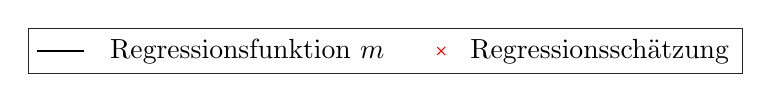
\begin{tikzpicture} 
    \begin{axis}[%
    legend columns=2,
    hide axis,
    xmin=10,
    xmax=50,
    ymin=0,
    ymax=0.4,
    legend style={draw=white!15!black,legend cell align=left,column sep=0.25cm}
    ]
    \addlegendimage{no markers,black}
    \addlegendentry{Regressionsfunktion $m \quad$};
     \addlegendimage{only marks,red,mark=x}
    \addlegendentry{Regressionsschätzung};
    \end{axis}
\end{tikzpicture}}
    \end{subfigure}
 \caption{Approximation der Regressionsfunktion $m(x) = \sin\big(\frac{\pi}{2} \cdot x^2\big)$ durch unseren Neuronale-Netze-Regressionsschätzer mit Parametern $d = 1$, $q = 2$, $R = 10^6$, $a = 3$, $N = 16$ und $M \in \{2,4,8,16\}$.}
 \label{fig:subfig.a.3}
\end{figure}
\begin{figure}
    \begin{subfigure}[b]{0.5\textwidth}
        \centering
        \scalebox{0.9}{
          % This file was created by tikzplotlib v0.9.0.
\begin{tikzpicture}

\begin{axis}[
tick align=outside,
tick pos=left,
title={$N = 2$, $M = 16$},
x grid style={white!69.0196078431373!black},
xmin=-3.34207441715318, xmax=3.35388433148518,
xtick style={color=black},
y grid style={white!69.0196078431373!black},
ymin=\ymin, ymax=\ymax,
ytick style={color=black}
]
\addplot [only marks, mark=x, draw=red, fill=red, colormap/viridis]
table{%
x                      y
2.76238288932011 -0.463161140690246
-2.97867143721344 1.11170632483828
1.34016626636584 0.328103900221429
-2.34602979642214 0.622726053028161
0.262724949982951 0.0932936493533496
0.761496100082008 0.816091744633529
-1.54231724537519 -0.556175431996082
2.48306325147965 -0.206831095835292
0.733875172149707 0.740106936985581
-1.60983185163084 -0.79607432496739
1.62079312559885 -0.801268369711307
-2.36695752001599 0.506958965874763
0.331351911188067 0.172439177397827
-2.43026358118505 0.122820282304857
0.485904436050117 0.348793128272332
-1.48211932367887 -0.26636541363796
0.896800847728478 0.977508873999964
1.29496171714908 0.478516181437511
0.145113687411967 0.0392009166832592
0.945128446218661 0.985127193977801
1.87976307195033 -0.720145744730991
1.84507362985819 -0.821088836712398
0.718091952323177 0.72496250146298
-0.293385227275351 0.133690161783831
-0.552300065715795 0.446007004779764
2.24848571942618 1.10690258854518
1.21759039268623 0.706705010760207
-1.89038986575959 -0.647337063259848
0.39439287977558 0.260129660964836
2.45284819380034 -0.031760800929817
-2.09586004651037 0.547186944572658
2.07310605318424 0.432987962213411
1.9212147978921 -0.42268229011325
-0.00395339221299285 -0.00611598362893603
-2.77449689108578 -0.359048475126319
-2.11498496761839 0.633593665755028
2.53583216813203 -0.578584942642351
-2.73507122380883 -0.591137264797007
-0.765007401567843 0.802265105569046
0.714237808352825 0.702728823520778
-1.8183117665159 -0.893160368520196
2.88647854344178 0.40196424771843
-2.06414860173947 0.391192263526636
0.238075170967647 0.107923152796403
0.708067946079868 0.693809941447383
-1.61406030798178 -0.80237832801808
-0.202146064743951 0.0661752597398166
-0.0539488252024247 0.00467641103052243
1.60117425795925 -0.759221498053604
0.80568451664324 0.883054978089857
-0.194699681607962 0.0657669957348491
1.00165525916385 1.01194312434435
-0.27973544086681 0.132993232649915
0.154269548048458 0.0448735976622029
0.951408249350171 0.97991469529514
-1.91282770827683 -0.494968830008023
1.72829730703384 -0.95265383141678
0.617192025230384 0.542773428611432
2.88199731082397 0.34710537510434
-1.66570083881295 -0.912376899827822
-0.202401155000559 0.0682922335779912
2.37385081559668 0.48990422515938
0.608600458192729 0.529933173808962
1.35575307509289 0.254137742303486
-0.517979014791838 0.402636606867873
1.10585773098792 0.954418295263262
2.67633017908538 -0.956372040261256
-1.79888360556407 -0.930612576634317
1.84419158326392 -0.818575560400849
2.81722807259938 -0.0679580540811622
-2.91258760942001 0.590570951739607
-1.70874248043343 -0.96103507381328
-2.29573847812122 0.903866093881658
1.60454110644872 -0.776723926277638
-2.5127004843436 -0.397618493618822
2.99048135154545 1.1476633703161
-0.662327904724169 0.616087437308203
2.43121659559824 0.0768393232081559
-1.86853437900319 -0.770367755639925
-0.354766801066255 0.189828591452233
2.06887091403722 0.430739557253923
0.571618684039537 0.468378160189806
-0.227051419851858 0.0962063754756209
0.0758984805427056 0.00440032773889413
0.443313161354085 0.29932150950588
-0.358084754486441 0.188772875750377
-1.83864625365714 -0.852579920290961
-2.31620543124488 0.793842041782595
-2.09263243577911 0.532118240625332
-2.6850542168812 -0.861870518303429
0.352058466381789 0.220971405181751
2.08632608421606 0.477348602468043
-0.845283966455336 0.906118498458334
-2.54813476418509 -0.623932706417743
-0.445653528089303 0.290127149013454
0.612047030832008 0.545395976628396
-0.447579206546175 0.31109107137991
1.86432740164422 -0.773626460452391
2.65131747712023 -1.01168670547952
2.21946463961013 1.02986209506946
1.22399698967933 0.715341207285279
-0.178206451306949 0.0586245704236229
1.09618825741951 0.948118498944542
-2.91949013666082 0.64450312547968
2.89486871101226 0.479669686064954
-1.96753600902662 -0.147333755833701
2.43756237577009 0.0856073247905787
1.84265940999664 -0.838022468427495
1.80083810632193 -0.893716240971356
-1.38638365328961 0.147189055446752
-1.68507716545645 -0.939834481817083
-0.427195842515467 0.284818756737455
2.09622660438393 0.529541549093289
-0.297722145169678 0.135173251906132
2.61252068404237 -1.06910605449426
-0.883924036489572 0.945811190170227
0.716352994180558 0.715537304482471
2.88419421813468 0.36779217404373
0.86077513344483 0.929738285328964
-2.72701070375638 -0.628031522435125
-0.218657454289729 0.0799483966696581
-0.991491937718017 1.00055015148373
0.193089291130048 0.0641434561039283
-1.29152274832121 0.485291119828091
-2.26643261861998 1.06097045595707
1.00973393250481 0.993537432134799
1.08815852934784 0.976706533638035
2.20283579999453 0.987892919550483
-2.20571103862358 1.00523980988622
1.79172184966819 -0.911241627435459
1.96061243043077 -0.230791033743328
0.879299614506912 0.946711959907842
-1.7704671253162 -0.958005077057877
-1.43147571356497 -0.0417584295740311
-0.489019094764946 0.35927964111015
0.250794436696388 0.0898393138889789
-0.135372266446698 0.0382754231576303
-0.195240647727783 0.0590833986655301
2.039044261186 0.202943022593416
2.22061419184541 1.01906787645756
1.9005237862606 -0.552821779931867
2.2668085118082 1.00022921431333
0.426052571622439 0.289248182255265
2.78421680003449 -0.278782101155095
0.639266089502806 0.559710312825165
0.623686446478088 0.546320626286095
-1.08421357755229 0.966156657009412
1.08722510470211 0.965170412392293
-2.68820586896783 -0.844143425526716
-2.19272147392835 0.959441060818508
-2.21854699456341 1.04904894369745
0.931207723348414 0.977239534127049
-1.94800444937197 -0.272444504243364
-0.953119060490716 0.981374988096537
-2.73413006500137 -0.59308615160625
-1.59759383930094 -0.753073020888769
2.78534594909577 -0.300131273778273
0.0548364150982064 0.0166918507026227
-2.09355288917141 0.536874786405437
0.138051190406785 0.0295550173370536
2.66105630346648 -1.0106443747517
2.194116084038 0.949641080213007
-0.647604786417679 0.59350062211445
-1.29679490415958 0.472555586334796
1.57037917615645 -0.689148205311893
-1.55709405118147 -0.611196066890769
-1.47460587205589 -0.234138180968196
-2.49548187492042 -0.285234790121326
2.18486456858416 0.911023620109852
-0.312606506278321 0.148741912637024
0.370717563659841 0.225099583267408
1.42026574616112 -0.0121022470556269
1.77893320278717 -0.951438230119911
-0.314951166058117 0.150300460688523
-1.89523466294521 -0.616636045163312
1.97239710916981 -0.124459609744577
-2.81401224103046 -0.104711576452358
2.68036961764771 -0.938675626295439
0.461867078865009 0.312234129758818
2.25233243070412 1.07890743526328
0.651392621841352 0.5903785269043
-1.49004249508606 -0.307677087605436
-1.22322045902457 0.693326609360435
0.197535354189919 0.0799343715089901
2.77246927708256 -0.410877450420673
-1.89302637305893 -0.629590947758836
0.0593902688586541 -0.00156337009736348
-0.937271379378934 0.980221925837238
1.61835206974311 -0.795169607318235
1.81719891859454 -0.850141931932902
-0.4526405381867 0.32138197823583
-1.77526500003398 -0.956024679598113
-2.59746323802687 -0.960521403143004
-1.80811041347663 -0.913497985823252
-1.36559489922371 0.224108649032642
0.592733507455263 0.4999420604217
2.23850098364661 1.07473088392933
-2.23061436692708 1.09110584221959
2.74913245028938 -0.564446119019849
1.09902506312488 0.951038376670626
};
\addplot [semithick, black]
table {%
-3 1
-2.99 0.995576734820054
-2.98 0.982404791977482
-2.97 0.960687140310815
-2.96 0.930698746339696
-2.95 0.892782465918225
-2.94 0.847344438774256
-2.93 0.794849046139829
-2.92 0.735813493407208
-2.91 0.670802080787205
-2.9 0.6004202253259
-2.89 0.525308297382294
-2.88 0.446135333817727
-2.87 0.363592688736647
-2.86 0.278387680690676
-2.85 0.191237292858769
-2.84 0.102861979893671
-2.83 0.0139796319282911
-2.82 -0.0747002572851044
-2.81 -0.162482174923344
-2.8 -0.248689887164819
-2.79 -0.332671415810564
-2.78 -0.413803662790115
-2.77 -0.491496656276015
-2.76000000000001 -0.565197396549224
-2.75000000000001 -0.63439328416361
-2.74000000000001 -0.698615117310616
-2.73000000000001 -0.7574396495474
-2.72000000000001 -0.810491703188593
-2.71000000000001 -0.857445837641644
-2.70000000000001 -0.898027575760592
-2.69000000000001 -0.932014194877928
-2.68000000000001 -0.959235092527838
-2.67000000000001 -0.979571739978357
-2.66000000000001 -0.992957239530362
-2.65000000000001 -0.999375504106505
-2.64000000000001 -0.998860079935072
-2.63000000000001 -0.991492635127341
-2.62000000000001 -0.977401138650261
-2.61000000000001 -0.956757755609883
-2.60000000000001 -0.929776485888277
-2.59000000000001 -0.896710574023413
-2.58000000000001 -0.857849718795458
-2.57000000000001 -0.813517111294285
-2.56000000000001 -0.764066330303094
-2.55000000000001 -0.709878123655345
-2.54000000000001 -0.651357103821107
-2.53000000000001 -0.588928385370132
-2.52000000000001 -0.523034191158988
-2.51000000000001 -0.454130453115695
-2.50000000000001 -0.382683432365167
-2.49000000000001 -0.309166382170306
-2.48000000000001 -0.234056275775223
-2.47000000000001 -0.157830619746354
-2.46000000000001 -0.0809643718325892
-2.45000000000001 -0.00392698072389465
-2.44000000000001 0.072820436603254
-2.43000000000001 0.148827765990005
-2.42000000000001 0.223658403427451
-2.41000000000001 0.296891588141009
-2.40000000000001 0.368124552684589
-2.39000000000001 0.43697448301218
-2.38000000000001 0.503080283168017
-2.37000000000001 0.56610414086275
-2.36000000000001 0.625732891772279
-2.35000000000001 0.681679181898872
-2.34000000000001 0.733682428763456
-2.33000000000001 0.781509583546624
-2.32000000000001 0.824955697558263
-2.31000000000001 0.863844297587357
-2.30000000000001 0.898027575760569
-2.29000000000002 0.927386400518292
-2.28000000000002 0.951830156198068
-2.27000000000002 0.971296419496836
-2.26000000000002 0.985750481765479
-2.25000000000002 0.995184726672186
-2.24000000000002 0.999617873256875
-2.23000000000002 0.999094094789406
-2.22000000000002 0.993682024142277
-2.21000000000002 0.983473656597255
-2.20000000000002 0.96858316112866
-2.19000000000002 0.949145611247931
-2.18000000000002 0.925315646459183
-2.17000000000002 0.897266075268519
-2.16000000000002 0.865186430515806
-2.15000000000002 0.829281487561826
-2.14000000000002 0.789769755571343
-2.13000000000002 0.746881951789148
-2.12000000000002 0.700859468316991
-2.11000000000002 0.651952840469899
-2.10000000000002 0.600420225325985
-2.09000000000002 0.546525898589853
-2.08000000000002 0.490538777371198
-2.07000000000002 0.432730975942088
-2.06000000000002 0.373376400983612
-2.05000000000002 0.31274939226965
-2.04000000000002 0.251123414166708
-2.03000000000002 0.188769802758421
-2.02000000000002 0.125956572835066
-2.01000000000002 0.062947288426061
-2.00000000000002 1.33870012014889e-13
-1.99000000000002 -0.062633749083271
-1.98000000000002 -0.124709844813965
-1.97000000000002 -0.185992451913749
-1.96000000000002 -0.246254789302508
-1.95000000000002 -0.305279831055913
-1.94000000000002 -0.3628609327075
-1.93000000000002 -0.418802383167873
-1.92000000000002 -0.472919882928091
-1.91000000000002 -0.525040949582032
-1.90000000000002 -0.575005252043164
-1.89000000000002 -0.622664875144035
-1.88000000000002 -0.667884516592001
-1.87000000000002 -0.710541618511978
-1.86000000000002 -0.750526436036607
-1.85000000000002 -0.787742045606543
-1.84000000000002 -0.822104295818981
-1.83000000000002 -0.85354170381174
-1.82000000000003 -0.881995300293982
-1.81000000000003 -0.907418426433774
-1.80000000000003 -0.929776485888198
-1.79000000000003 -0.949046655314642
-1.78000000000003 -0.965217556733346
-1.77000000000003 -0.978288895122437
-1.76000000000003 -0.988271064618766
-1.75000000000003 -0.995184726672183
-1.74000000000003 -0.99906036345861
-1.73000000000003 -0.999937809799883
-1.72000000000003 -0.997865766766904
-1.71000000000003 -0.992901300058717
-1.70000000000003 -0.985109326154799
-1.69000000000003 -0.974562089132473
-1.68000000000003 -0.961338630927184
-1.67000000000003 -0.945524257691589
-1.66000000000003 -0.92721000478115
-1.65000000000003 -0.906492102760418
-1.64000000000003 -0.883471446686396
-1.63000000000003 -0.858253070784441
-1.62000000000003 -0.830945630488965
-1.61000000000003 -0.801660893676759
-1.60000000000003 -0.770513242775885
-1.59000000000003 -0.737619189288572
-1.58000000000003 -0.703096902123257
-1.57000000000003 -0.667065750989361
-1.56000000000003 -0.629645865969377
-1.55000000000003 -0.590957714246878
-1.54000000000003 -0.5511216948366
-1.53000000000003 -0.510257752034371
-1.52000000000003 -0.468485008180726
-1.51000000000003 -0.425921416212823
-1.50000000000003 -0.382683432365229
-1.49000000000003 -0.338885709271396
-1.48000000000003 -0.29464080961443
-1.47000000000003 -0.250058940378286
-1.46000000000003 -0.205247707658841
-1.45000000000003 -0.16031189190854
-1.44000000000003 -0.115353243408457
-1.43000000000003 -0.0704702976877775
-1.42000000000003 -0.0257582105426693
-1.41000000000003 0.018691387755514
-1.40000000000003 0.0627905195291638
-1.39000000000003 0.106454968557562
-1.38000000000003 0.149604371296494
-1.37000000000003 0.192162291056312
-1.36000000000003 0.234056275774993
-1.35000000000004 0.275217900052248
-1.34000000000004 0.315582792135412
-1.33000000000004 0.355090646567928
-1.32000000000004 0.393685223226887
-1.31000000000004 0.431314333487567
-1.30000000000004 0.467929814260443
-1.29000000000004 0.503487490649953
-1.28000000000004 0.537947127984647
-1.27000000000004 0.571272373965398
-1.26000000000004 0.603430691672474
-1.25000000000004 0.634393284163532
-1.24000000000004 0.664135011383361
-1.23000000000004 0.692634300092632
-1.22000000000004 0.719873047507249
-1.21000000000004 0.745836519322339
-1.20000000000004 0.770513242775697
-1.19000000000004 0.79389489538482
-1.18000000000004 0.815976189969678
-1.17000000000004 0.836754756550324
-1.16000000000004 0.856231021684473
-1.15000000000004 0.87440808578545
-1.14000000000004 0.891291598935659
-1.13000000000004 0.906889635684947
-1.12000000000004 0.921212569297285
-1.11000000000004 0.93427294588298
-1.10000000000004 0.9460853588275
-1.09000000000004 0.956666323901834
-1.08000000000004 0.966034155413461
-1.07000000000004 0.974208843731348
-1.06000000000004 0.981211934493193
-1.05000000000004 0.987066409778344
-1.04000000000004 0.991796571505593
-1.03000000000004 0.995427927291427
-1.02000000000004 0.997987078981312
-1.01000000000004 0.999501614044331
-1.00000000000004 1
-0.990000000000043 0.999511482025296
-0.980000000000043 0.998065983870084
-0.970000000000043 0.995694012190007
-0.960000000000043 0.992426564387702
-0.950000000000044 0.988295040035889
-0.940000000000044 0.983331155939389
-0.930000000000044 0.977566864877576
-0.920000000000044 0.971034278054095
-0.910000000000045 0.963765591266851
-0.900000000000045 0.955793014798367
-0.890000000000045 0.94714870701456
-0.880000000000045 0.937864711648732
-0.870000000000045 0.927972898737259
-0.860000000000046 0.917504909163832
-0.850000000000046 0.906492102760406
-0.840000000000046 0.894965509904969
-0.830000000000046 0.882955786549018
-0.820000000000046 0.870493172601118
-0.810000000000047 0.857607453587072
-0.800000000000047 0.844327925502078
-0.790000000000047 0.830683362765738
-0.780000000000047 0.816701989186866
-0.770000000000048 0.802411451841723
-0.760000000000048 0.787838797766522
-0.750000000000048 0.773010453362809
-0.740000000000048 0.757952206412552
-0.730000000000048 0.742689190598499
-0.720000000000049 0.727245872424471
-0.710000000000049 0.711646040429847
-0.700000000000049 0.695912796592392
-0.690000000000049 0.68006854981388
-0.680000000000049 0.664135011383549
-0.67000000000005 0.648133192315342
-0.66000000000005 0.632083402456062
-0.65000000000005 0.61600525126299
-0.64000000000005 0.599917650151169
-0.630000000000051 0.583838816312412
-0.620000000000051 0.567786277910133
-0.610000000000051 0.551776880556293
-0.600000000000051 0.535826794979078
-0.590000000000051 0.519951525792427
-0.580000000000052 0.504165921281037
-0.570000000000052 0.488484184117171
-0.560000000000052 0.472919882928293
-0.550000000000052 0.457485964637341
-0.540000000000052 0.442194767500267
-0.530000000000053 0.427058034768333
-0.520000000000053 0.4120869289055
-0.510000000000053 0.397292046294142
-0.500000000000053 0.382683432365167
-0.490000000000054 0.368270597091477
-0.480000000000054 0.354062530786545
-0.470000000000054 0.340067720152659
-0.460000000000054 0.326294164526146
-0.450000000000054 0.312749392269599
-0.440000000000055 0.299440477263786
-0.430000000000055 0.286374055454505
-0.420000000000055 0.273556341412193
-0.410000000000055 0.260993144864562
-0.400000000000055 0.248689887164922
-0.390000000000056 0.23665161766118
-0.380000000000056 0.22488302993274
-0.370000000000056 0.213388477864702
-0.360000000000056 0.202171991530836
-0.350000000000056 0.191237292858801
-0.340000000000057 0.180587811053027
-0.330000000000057 0.170226697752469
-0.320000000000057 0.160156841902239
-0.310000000000057 0.150380884319751
-0.300000000000058 0.140901231937636
-0.290000000000058 0.131720071707145
-0.280000000000058 0.122839384147215
-0.270000000000058 0.114260956525697
-0.260000000000058 0.105986395660502
-0.250000000000059 0.0980171403296064
-0.240000000000059 0.0903544732799798
-0.230000000000059 0.0829995328265039
-0.220000000000059 0.0759533240329385
-0.210000000000059 0.0692167294678623
-0.20000000000006 0.0627905195293508
-0.19000000000006 0.0566753623329036
-0.18000000000006 0.0508718331578319
-0.17000000000006 0.0453804234479493
-0.160000000000061 0.0402015493629836
-0.150000000000061 0.0353355598776498
-0.140000000000061 0.0307827444257893
-0.130000000000061 0.0265433400874004
-0.120000000000061 0.0226175383167529
-0.110000000000062 0.019005491210107
-0.100000000000062 0.0157073173118401
-0.090000000000062 0.012723106958029
-0.0800000000000622 0.0100529271567463
-0.0700000000000625 0.00769682600450373
-0.0600000000000627 0.00565483663842069
-0.0500000000000629 0.00392698072381588
-0.0400000000000631 0.00251327147701166
-0.0300000000000633 0.00141371622321359
-0.0200000000000635 0.000628318489380248
-0.0100000000000637 0.000157079632035528
-6.3948846218409e-14 6.42370078682459e-27
0.00999999999993584 0.00015707963203151
0.0199999999999356 0.000628318489372212
0.0299999999999354 0.00141371622320154
0.0399999999999352 0.00251327147699558
0.049999999999935 0.00392698072379579
0.0599999999999348 0.00565483663839659
0.0699999999999346 0.00769682600447561
0.0799999999999343 0.0100529271567142
0.0899999999999341 0.0127231069579928
0.0999999999999339 0.0157073173117999
0.109999999999934 0.0190054912100628
0.119999999999933 0.0226175383167047
0.129999999999933 0.0265433400873482
0.139999999999933 0.0307827444257331
0.149999999999933 0.0353355598775896
0.159999999999933 0.0402015493629194
0.169999999999932 0.045380423447881
0.179999999999932 0.0508718331577597
0.189999999999932 0.0566753623328273
0.199999999999932 0.0627905195292706
0.209999999999932 0.0692167294677781
0.219999999999931 0.0759533240328503
0.229999999999931 0.0829995328264118
0.239999999999931 0.0903544732798837
0.249999999999931 0.0980171403295065
0.259999999999931 0.105986395660398
0.26999999999993 0.114260956525589
0.27999999999993 0.122839384147103
0.28999999999993 0.131720071707029
0.29999999999993 0.140901231937517
0.309999999999929 0.150380884319628
0.319999999999929 0.160156841902112
0.329999999999929 0.170226697752338
0.339999999999929 0.180587811052893
0.349999999999929 0.191237292858663
0.359999999999928 0.202171991530694
0.369999999999928 0.213388477864557
0.379999999999928 0.224883029932591
0.389999999999928 0.236651617661028
0.399999999999928 0.248689887164767
0.409999999999927 0.260993144864403
0.419999999999927 0.273556341412031
0.429999999999927 0.28637405545434
0.439999999999927 0.299440477263618
0.449999999999926 0.312749392269427
0.459999999999926 0.326294164525971
0.469999999999926 0.340067720152481
0.479999999999926 0.354062530786364
0.489999999999926 0.368270597091294
0.499999999999925 0.382683432364981
0.509999999999925 0.397292046293954
0.519999999999925 0.412086928905309
0.529999999999925 0.42705803476814
0.539999999999925 0.442194767500072
0.549999999999924 0.457485964637144
0.559999999999924 0.472919882928095
0.569999999999924 0.488484184116971
0.579999999999924 0.504165921280836
0.589999999999923 0.519951525792225
0.599999999999923 0.535826794978874
0.609999999999923 0.551776880556088
0.619999999999923 0.567786277909928
0.629999999999923 0.583838816312206
0.639999999999922 0.599917650150963
0.649999999999922 0.616005251262785
0.659999999999922 0.632083402455857
0.669999999999922 0.648133192315137
0.679999999999922 0.664135011383345
0.689999999999921 0.680068549813677
0.699999999999921 0.69591279659219
0.709999999999921 0.711646040429646
0.719999999999921 0.727245872424273
0.72999999999992 0.742689190598303
0.73999999999992 0.757952206412358
0.74999999999992 0.773010453362617
0.75999999999992 0.787838797766334
0.76999999999992 0.802411451841539
0.779999999999919 0.816701989186685
0.789999999999919 0.830683362765561
0.799999999999919 0.844327925501906
0.809999999999919 0.857607453586905
0.819999999999919 0.870493172600956
0.829999999999918 0.882955786548861
0.839999999999918 0.894965509904818
0.849999999999918 0.906492102760262
0.859999999999918 0.917504909163694
0.869999999999918 0.927972898737128
0.879999999999917 0.93786471164861
0.889999999999917 0.947148707014445
0.899999999999917 0.955793014798261
0.909999999999917 0.963765591266753
0.919999999999916 0.971034278054007
0.929999999999916 0.977566864877497
0.939999999999916 0.98333115593932
0.949999999999916 0.988295040035831
0.959999999999916 0.992426564387655
0.969999999999915 0.995694012189971
0.979999999999915 0.99806598387006
0.989999999999915 0.999511482025283
0.999999999999915 1
1.00999999999991 0.999501614044344
1.01999999999991 0.997987078981338
1.02999999999991 0.995427927291467
1.03999999999991 0.991796571505646
1.04999999999991 0.987066409778411
1.05999999999991 0.981211934493276
1.06999999999991 0.974208843731445
1.07999999999991 0.966034155413573
1.08999999999991 0.956666323901962
1.09999999999991 0.946085358827643
1.10999999999991 0.934272945883139
1.11999999999991 0.92121256929746
1.12999999999991 0.906889635685138
1.13999999999991 0.891291598935866
1.14999999999991 0.874408085785674
1.15999999999991 0.856231021684713
1.16999999999991 0.836754756550582
1.17999999999991 0.815976189969952
1.18999999999991 0.793894895385111
1.19999999999991 0.770513242776004
1.20999999999991 0.745836519322663
1.21999999999991 0.719873047507589
1.22999999999991 0.692634300092988
1.23999999999991 0.664135011383733
1.24999999999991 0.63439328416392
1.25999999999991 0.603430691672878
1.26999999999991 0.571272373965817
1.27999999999991 0.537947127985081
1.28999999999991 0.503487490650401
1.29999999999991 0.467929814260904
1.30999999999991 0.431314333488042
1.31999999999991 0.393685223227375
1.32999999999991 0.355090646568427
1.33999999999991 0.315582792135923
1.34999999999991 0.27521790005277
1.35999999999991 0.234056275775525
1.36999999999991 0.192162291056853
1.37999999999991 0.149604371297043
1.38999999999991 0.106454968558117
1.39999999999991 0.0627905195297253
1.40999999999991 0.0186913877560805
1.41999999999991 -0.0257582105420993
1.42999999999991 -0.0704702976872039
1.43999999999991 -0.115353243407883
1.44999999999991 -0.160311891907964
1.4599999999999 -0.205247707658268
1.4699999999999 -0.250058940377715
1.4799999999999 -0.294640809613862
1.4899999999999 -0.338885709270833
1.4999999999999 -0.382683432364672
1.5099999999999 -0.425921416212274
1.5199999999999 -0.468485008180186
1.5299999999999 -0.510257752033843
1.5399999999999 -0.551121694836084
1.5499999999999 -0.590957714246376
1.5599999999999 -0.62964586596889
1.5699999999999 -0.667065750988891
1.5799999999999 -0.703096902122806
1.5899999999999 -0.73761918928814
1.5999999999999 -0.770513242775475
1.6099999999999 -0.801660893676373
1.6199999999999 -0.830945630488602
1.6299999999999 -0.858253070784105
1.6399999999999 -0.883471446686087
1.6499999999999 -0.906492102760138
1.6599999999999 -0.9272100047809
1.6699999999999 -0.945524257691371
1.6799999999999 -0.961338630926998
1.6899999999999 -0.974562089132321
1.6999999999999 -0.985109326154682
1.7099999999999 -0.992901300058635
1.7199999999999 -0.997865766766859
1.7299999999999 -0.999937809799876
1.7399999999999 -0.99906036345864
1.7499999999999 -0.995184726672251
1.7599999999999 -0.988271064618874
1.7699999999999 -0.978288895122584
1.7799999999999 -0.965217556733533
1.7899999999999 -0.949046655314868
1.7999999999999 -0.929776485888465
1.8099999999999 -0.90741842643408
1.8199999999999 -0.881995300294327
1.8299999999999 -0.853541703812123
1.8399999999999 -0.822104295819402
1.8499999999999 -0.787742045607001
1.8599999999999 -0.750526436037101
1.8699999999999 -0.710541618512508
1.8799999999999 -0.667884516592564
1.8899999999999 -0.622664875144629
1.8999999999999 -0.575005252043788
1.9099999999999 -0.525040949582685
1.9199999999999 -0.47291988292877
1.92999999999989 -0.418802383168577
1.93999999999989 -0.362860932708227
1.94999999999989 -0.305279831056659
1.95999999999989 -0.246254789303272
1.96999999999989 -0.185992451914526
1.97999999999989 -0.124709844814754
1.98999999999989 -0.0626337490840697
1.99999999999989 -6.69931457813724e-13
2.00999999999989 0.0629472884252544
2.01999999999989 0.12595657283426
2.02999999999989 0.18876980275762
2.03999999999989 0.251123414165916
2.04999999999989 0.312749392268867
2.05999999999989 0.373376400982844
2.06999999999989 0.432730975941339
2.07999999999989 0.490538777370471
2.08999999999989 0.54652589858915
2.09999999999989 0.600420225325311
2.10999999999989 0.651952840469257
2.11999999999989 0.700859468316383
2.12999999999989 0.746881951788579
2.13999999999989 0.789769755570817
2.14999999999989 0.829281487561343
2.15999999999989 0.865186430515371
2.16999999999989 0.897266075268134
2.17999999999989 0.925315646458851
2.18999999999989 0.949145611247653
2.19999999999989 0.968583161128441
2.20999999999989 0.983473656597094
2.21999999999989 0.993682024142177
2.22999999999989 0.999094094789368
2.23999999999989 0.9996178732569
2.24999999999989 0.995184726672274
2.25999999999989 0.985750481765632
2.26999999999989 0.971296419497053
2.27999999999989 0.951830156198348
2.28999999999989 0.927386400518636
2.29999999999989 0.898027575760974
2.30999999999989 0.863844297587825
2.31999999999989 0.82495569755879
2.32999999999989 0.781509583547208
2.33999999999989 0.733682428764095
2.34999999999989 0.681679181899562
2.35999999999989 0.625732891773019
2.36999999999989 0.566104140863535
2.37999999999989 0.503080283168843
2.38999999999989 0.436974483013044
2.39999999999988 0.368124552685486
2.40999999999988 0.296891588141934
2.41999999999988 0.2236584034284
2.42999999999988 0.148827765990971
2.43999999999988 0.072820436604232
2.44999999999988 -0.00392698072291233
2.45999999999988 -0.0809643718316048
2.46999999999988 -0.157830619745374
2.47999999999988 -0.234056275774253
2.48999999999988 -0.309166382169355
2.49999999999988 -0.382683432364238
2.50999999999988 -0.454130453114798
2.51999999999988 -0.523034191158123
2.52999999999988 -0.58892838536931
2.53999999999988 -0.651357103820333
2.54999999999988 -0.709878123654623
2.55999999999988 -0.764066330302429
2.56999999999988 -0.813517111293685
2.57999999999988 -0.857849718794925
2.58999999999988 -0.896710574022952
2.59999999999988 -0.929776485887892
2.60999999999988 -0.956757755609577
2.61999999999988 -0.977401138650039
2.62999999999988 -0.991492635127203
2.63999999999988 -0.998860079935021
2.64999999999988 -0.999375504106543
2.65999999999988 -0.992957239530489
2.66999999999988 -0.979571739978573
2.67999999999988 -0.959235092528142
2.68999999999988 -0.93201419487832
2.69999999999988 -0.898027575761069
2.70999999999988 -0.857445837642205
2.71999999999988 -0.810491703189233
2.72999999999988 -0.757439649548115
2.73999999999988 -0.698615117311402
2.74999999999988 -0.634393284164464
2.75999999999988 -0.565197396550139
2.76999999999988 -0.491496656276984
2.77999999999988 -0.413803662791132
2.78999999999988 -0.332671415811622
2.79999999999988 -0.248689887165909
2.80999999999988 -0.162482174924459
2.81999999999988 -0.0747002572862345
2.82999999999988 0.0139796319271562
2.83999999999988 0.102861979892536
2.84999999999988 0.191237292857646
2.85999999999988 0.278387680689572
2.86999999999987 0.36359268873557
2.87999999999987 0.44613533381669
2.88999999999987 0.525308297381304
2.89999999999987 0.600420225324967
2.90999999999987 0.670802080786339
2.91999999999987 0.735813493406414
2.92999999999987 0.794849046139114
2.93999999999987 0.847344438773628
2.94999999999987 0.892782465917691
2.95999999999987 0.930698746339261
2.96999999999987 0.960687140310484
2.97999999999987 0.982404791977258
2.98999999999987 0.995576734819941
};
\end{axis}

\end{tikzpicture}
}
        \label{fig:subfig4n2m16}
    \end{subfigure}
    \begin{subfigure}[b]{0.5\textwidth}
    \centering
    \scalebox{0.9}{
           % This file was created by tikzplotlib v0.9.0.
\begin{tikzpicture}

\begin{axis}[
tick align=outside,
tick pos=left,
title={$N = 4$, $M = 16$},
x grid style={white!69.0196078431373!black},
xmin=-3.34207441715318, xmax=3.35388433148518,
xtick style={color=black},
y grid style={white!69.0196078431373!black},
ymin=\ymin, ymax=\ymax,
ytick style={color=black}
]
\addplot [only marks, mark=x, draw=red, fill=red, colormap/viridis]
table{%
x                      y
2.76238288932011 -0.442378439315154
-2.97867143721344 1.08538845927425
1.34016626636584 0.327261453184745
-2.34602979642214 0.640926577041887
0.262724949982951 0.103171160678765
0.761496100082008 0.830101018400724
-1.54231724537519 -0.555877695387648
2.48306325147965 -0.221769612457636
0.733875172149707 0.750665088575188
-1.60983185163084 -0.80075788705249
1.62079312559885 -0.810325215103169
-2.36695752001599 0.527404885158905
0.331351911188067 0.172746051065665
-2.43026358118505 0.137182293655737
0.485904436050117 0.347936419037903
-1.48211932367887 -0.261207033482822
0.896800847728478 0.98450445387718
1.29496171714908 0.463228249271119
0.145113687411967 0.0271930203670559
0.945128446218661 0.983992618737439
1.87976307195033 -0.727608585314711
1.84507362985819 -0.831840919398742
0.718091952323177 0.730610225651024
-0.293385227275351 0.133261402481247
-0.552300065715795 0.443308062460882
2.24848571942618 1.11280483326494
1.21759039268623 0.708416545551247
-1.89038986575959 -0.638529384885081
0.39439287977558 0.259288828973216
2.45284819380034 0.0185259704359327
-2.09586004651037 0.54350035091972
2.07310605318424 0.447113140899451
1.9212147978921 -0.440709277329445
-0.00395339221299285 0.00711609981973051
-2.77449689108578 -0.343396849431168
-2.11498496761839 0.628355781983405
2.53583216813203 -0.550979439442001
-2.73507122380883 -0.584877733716031
-0.765007401567843 0.78737620009943
0.714237808352825 0.693661411061542
-1.8183117665159 -0.89402839023003
2.88647854344178 0.407757990100539
-2.06414860173947 0.386148280140304
0.238075170967647 0.10901521701905
0.708067946079868 0.703014276558013
-1.61406030798178 -0.807797284719958
-0.202146064743951 0.0678697360369753
-0.0539488252024247 0.0188912236605266
1.60117425795925 -0.76501537375489
0.80568451664324 0.864565152284568
-0.194699681607962 0.0611651028238597
1.00165525916385 1.01927321917248
-0.27973544086681 0.141942899900414
0.154269548048458 0.0384247557721217
0.951408249350171 0.965693989990858
-1.91282770827683 -0.485833358021669
1.72829730703384 -0.96359965291153
0.617192025230384 0.51710439780267
2.88199731082397 0.389811709842681
-1.66570083881295 -0.920905778004681
-0.202401155000559 0.0682689820095419
2.37385081559668 0.427570992760527
0.608600458192729 0.521834542931789
1.35575307509289 0.253297682241056
-0.517979014791838 0.410113188869849
1.10585773098792 0.974144467796221
2.67633017908538 -0.918733206897897
-1.79888360556407 -0.925989577561093
1.84419158326392 -0.815555218794237
2.81722807259938 -0.0891790357107135
-2.91258760942001 0.602311435729543
-1.70874248043343 -0.970538757012858
-2.29573847812122 0.914061195707775
1.60454110644872 -0.765156973061228
-2.5127004843436 -0.402661643748677
2.99048135154545 1.11331023366585
-0.662327904724169 0.621230448607462
2.43121659559824 0.0812050982269387
-1.86853437900319 -0.762183309292449
-0.354766801066255 0.185392079073888
2.06887091403722 0.426386824213542
0.571618684039537 0.454611353789515
-0.227051419851858 0.0931526937758619
0.0758984805427056 0.0056152015571804
0.443313161354085 0.300031342940188
-0.358084754486441 0.196229857993746
-1.83864625365714 -0.846445927680529
-2.31620543124488 0.814390067214484
-2.09263243577911 0.530394121763122
-2.6850542168812 -0.869273283586313
0.352058466381789 0.230190495042693
2.08632608421606 0.45704626219053
-0.845283966455336 0.92317012326721
-2.54813476418509 -0.635287215267574
-0.445653528089303 0.282604382106913
0.612047030832008 0.528083053031089
-0.447579206546175 0.306884936200165
1.86432740164422 -0.767579046461308
2.65131747712023 -1.01778461816141
2.21946463961013 1.02649371404683
1.22399698967933 0.717913380418641
-0.178206451306949 0.0583316714223784
1.09618825741951 0.937900705452212
-2.91949013666082 0.649188325001753
2.89486871101226 0.419062405997388
-1.96753600902662 -0.144892031998592
2.43756237577009 0.101606735599505
1.84265940999664 -0.850966759628998
1.80083810632193 -0.892361430928038
-1.38638365328961 0.152026201693138
-1.68507716545645 -0.942905546421048
-0.427195842515467 0.284521814490197
2.09622660438393 0.535235110288535
-0.297722145169678 0.118993095592654
2.61252068404237 -1.00904949206573
-0.883924036489572 0.958818743384695
0.716352994180558 0.704725193957479
2.88419421813468 0.387813652690027
0.86077513344483 0.937291301584362
-2.72701070375638 -0.623471558073663
-0.218657454289729 0.0830032835043427
-0.991491937718017 1.00952974745136
0.193089291130048 0.0522288466542998
-1.29152274832121 0.481063221414277
-2.26643261861998 1.0590688006713
1.00973393250481 0.987431921895693
1.08815852934784 0.975847395112787
2.20283579999453 0.958294124011751
-2.20571103862358 0.996948836780345
1.79172184966819 -0.90586783688842
1.96061243043077 -0.213233851770111
0.879299614506912 0.942699167354449
-1.7704671253162 -0.959438945061509
-1.43147571356497 -0.0383176962090818
-0.489019094764946 0.357308848762798
0.250794436696388 0.0811191618210141
-0.135372266446698 0.0357489508488429
-0.195240647727783 0.0603957472165774
2.039044261186 0.254242221464334
2.22061419184541 1.01765231480234
1.9005237862606 -0.562346442492453
2.2668085118082 1.04300712551641
0.426052571622439 0.29168060347465
2.78421680003449 -0.29117760968086
0.639266089502806 0.548999958357525
0.623686446478088 0.543007876546004
-1.08421357755229 0.958338358922294
1.08722510470211 0.9645127407397
-2.68820586896783 -0.853480332839502
-2.19272147392835 0.953833450888038
-2.21854699456341 1.03751278884941
0.931207723348414 0.968899413914248
-1.94800444937197 -0.273437876116273
-0.953119060490716 0.997256818115465
-2.73413006500137 -0.590069521779894
-1.59759383930094 -0.75976768526822
2.78534594909577 -0.2833850905918
0.0548364150982064 0.0349579657061632
-2.09355288917141 0.532447448799769
0.138051190406785 0.0186362982932771
2.66105630346648 -1.00836883709729
2.194116084038 0.956730663513405
-0.647604786417679 0.581481139485903
-1.29679490415958 0.475202224439472
1.57037917615645 -0.701871397585613
-1.55709405118147 -0.616296384729198
-1.47460587205589 -0.227525951117438
-2.49548187492042 -0.281697232492489
2.18486456858416 0.919863764595074
-0.312606506278321 0.138399344535342
0.370717563659841 0.247042106693162
1.42026574616112 0.000214795141129205
1.77893320278717 -0.945092892574662
-0.314951166058117 0.158203140572034
-1.89523466294521 -0.610564271200204
1.97239710916981 -0.122669940570274
-2.81401224103046 -0.0846317960023732
2.68036961764771 -0.909121338663274
0.461867078865009 0.305768386265064
2.25233243070412 1.08167276797902
0.651392621841352 0.591393699794396
-1.49004249508606 -0.30358236318914
-1.22322045902457 0.696470558037947
0.197535354189919 0.0813104166539383
2.77246927708256 -0.357485358981014
-1.89302637305893 -0.620831537469806
0.0593902688586541 -0.0105153438112986
-0.937271379378934 0.993666799040502
1.61835206974311 -0.775640119715474
1.81719891859454 -0.90041631481897
-0.4526405381867 0.330545621296503
-1.77526500003398 -0.95851465720402
-2.59746323802687 -0.979486926417859
-1.80811041347663 -0.913106955399545
-1.36559489922371 0.225207141839538
0.592733507455263 0.482520018295919
2.23850098364661 1.08121227359546
-2.23061436692708 1.08062337169829
2.74913245028938 -0.525463471487725
1.09902506312488 0.952230635702206
};
\addplot [semithick, black]
table {%
-3 1
-2.99 0.995576734820054
-2.98 0.982404791977482
-2.97 0.960687140310815
-2.96 0.930698746339696
-2.95 0.892782465918225
-2.94 0.847344438774256
-2.93 0.794849046139829
-2.92 0.735813493407208
-2.91 0.670802080787205
-2.9 0.6004202253259
-2.89 0.525308297382294
-2.88 0.446135333817727
-2.87 0.363592688736647
-2.86 0.278387680690676
-2.85 0.191237292858769
-2.84 0.102861979893671
-2.83 0.0139796319282911
-2.82 -0.0747002572851044
-2.81 -0.162482174923344
-2.8 -0.248689887164819
-2.79 -0.332671415810564
-2.78 -0.413803662790115
-2.77 -0.491496656276015
-2.76000000000001 -0.565197396549224
-2.75000000000001 -0.63439328416361
-2.74000000000001 -0.698615117310616
-2.73000000000001 -0.7574396495474
-2.72000000000001 -0.810491703188593
-2.71000000000001 -0.857445837641644
-2.70000000000001 -0.898027575760592
-2.69000000000001 -0.932014194877928
-2.68000000000001 -0.959235092527838
-2.67000000000001 -0.979571739978357
-2.66000000000001 -0.992957239530362
-2.65000000000001 -0.999375504106505
-2.64000000000001 -0.998860079935072
-2.63000000000001 -0.991492635127341
-2.62000000000001 -0.977401138650261
-2.61000000000001 -0.956757755609883
-2.60000000000001 -0.929776485888277
-2.59000000000001 -0.896710574023413
-2.58000000000001 -0.857849718795458
-2.57000000000001 -0.813517111294285
-2.56000000000001 -0.764066330303094
-2.55000000000001 -0.709878123655345
-2.54000000000001 -0.651357103821107
-2.53000000000001 -0.588928385370132
-2.52000000000001 -0.523034191158988
-2.51000000000001 -0.454130453115695
-2.50000000000001 -0.382683432365167
-2.49000000000001 -0.309166382170306
-2.48000000000001 -0.234056275775223
-2.47000000000001 -0.157830619746354
-2.46000000000001 -0.0809643718325892
-2.45000000000001 -0.00392698072389465
-2.44000000000001 0.072820436603254
-2.43000000000001 0.148827765990005
-2.42000000000001 0.223658403427451
-2.41000000000001 0.296891588141009
-2.40000000000001 0.368124552684589
-2.39000000000001 0.43697448301218
-2.38000000000001 0.503080283168017
-2.37000000000001 0.56610414086275
-2.36000000000001 0.625732891772279
-2.35000000000001 0.681679181898872
-2.34000000000001 0.733682428763456
-2.33000000000001 0.781509583546624
-2.32000000000001 0.824955697558263
-2.31000000000001 0.863844297587357
-2.30000000000001 0.898027575760569
-2.29000000000002 0.927386400518292
-2.28000000000002 0.951830156198068
-2.27000000000002 0.971296419496836
-2.26000000000002 0.985750481765479
-2.25000000000002 0.995184726672186
-2.24000000000002 0.999617873256875
-2.23000000000002 0.999094094789406
-2.22000000000002 0.993682024142277
-2.21000000000002 0.983473656597255
-2.20000000000002 0.96858316112866
-2.19000000000002 0.949145611247931
-2.18000000000002 0.925315646459183
-2.17000000000002 0.897266075268519
-2.16000000000002 0.865186430515806
-2.15000000000002 0.829281487561826
-2.14000000000002 0.789769755571343
-2.13000000000002 0.746881951789148
-2.12000000000002 0.700859468316991
-2.11000000000002 0.651952840469899
-2.10000000000002 0.600420225325985
-2.09000000000002 0.546525898589853
-2.08000000000002 0.490538777371198
-2.07000000000002 0.432730975942088
-2.06000000000002 0.373376400983612
-2.05000000000002 0.31274939226965
-2.04000000000002 0.251123414166708
-2.03000000000002 0.188769802758421
-2.02000000000002 0.125956572835066
-2.01000000000002 0.062947288426061
-2.00000000000002 1.33870012014889e-13
-1.99000000000002 -0.062633749083271
-1.98000000000002 -0.124709844813965
-1.97000000000002 -0.185992451913749
-1.96000000000002 -0.246254789302508
-1.95000000000002 -0.305279831055913
-1.94000000000002 -0.3628609327075
-1.93000000000002 -0.418802383167873
-1.92000000000002 -0.472919882928091
-1.91000000000002 -0.525040949582032
-1.90000000000002 -0.575005252043164
-1.89000000000002 -0.622664875144035
-1.88000000000002 -0.667884516592001
-1.87000000000002 -0.710541618511978
-1.86000000000002 -0.750526436036607
-1.85000000000002 -0.787742045606543
-1.84000000000002 -0.822104295818981
-1.83000000000002 -0.85354170381174
-1.82000000000003 -0.881995300293982
-1.81000000000003 -0.907418426433774
-1.80000000000003 -0.929776485888198
-1.79000000000003 -0.949046655314642
-1.78000000000003 -0.965217556733346
-1.77000000000003 -0.978288895122437
-1.76000000000003 -0.988271064618766
-1.75000000000003 -0.995184726672183
-1.74000000000003 -0.99906036345861
-1.73000000000003 -0.999937809799883
-1.72000000000003 -0.997865766766904
-1.71000000000003 -0.992901300058717
-1.70000000000003 -0.985109326154799
-1.69000000000003 -0.974562089132473
-1.68000000000003 -0.961338630927184
-1.67000000000003 -0.945524257691589
-1.66000000000003 -0.92721000478115
-1.65000000000003 -0.906492102760418
-1.64000000000003 -0.883471446686396
-1.63000000000003 -0.858253070784441
-1.62000000000003 -0.830945630488965
-1.61000000000003 -0.801660893676759
-1.60000000000003 -0.770513242775885
-1.59000000000003 -0.737619189288572
-1.58000000000003 -0.703096902123257
-1.57000000000003 -0.667065750989361
-1.56000000000003 -0.629645865969377
-1.55000000000003 -0.590957714246878
-1.54000000000003 -0.5511216948366
-1.53000000000003 -0.510257752034371
-1.52000000000003 -0.468485008180726
-1.51000000000003 -0.425921416212823
-1.50000000000003 -0.382683432365229
-1.49000000000003 -0.338885709271396
-1.48000000000003 -0.29464080961443
-1.47000000000003 -0.250058940378286
-1.46000000000003 -0.205247707658841
-1.45000000000003 -0.16031189190854
-1.44000000000003 -0.115353243408457
-1.43000000000003 -0.0704702976877775
-1.42000000000003 -0.0257582105426693
-1.41000000000003 0.018691387755514
-1.40000000000003 0.0627905195291638
-1.39000000000003 0.106454968557562
-1.38000000000003 0.149604371296494
-1.37000000000003 0.192162291056312
-1.36000000000003 0.234056275774993
-1.35000000000004 0.275217900052248
-1.34000000000004 0.315582792135412
-1.33000000000004 0.355090646567928
-1.32000000000004 0.393685223226887
-1.31000000000004 0.431314333487567
-1.30000000000004 0.467929814260443
-1.29000000000004 0.503487490649953
-1.28000000000004 0.537947127984647
-1.27000000000004 0.571272373965398
-1.26000000000004 0.603430691672474
-1.25000000000004 0.634393284163532
-1.24000000000004 0.664135011383361
-1.23000000000004 0.692634300092632
-1.22000000000004 0.719873047507249
-1.21000000000004 0.745836519322339
-1.20000000000004 0.770513242775697
-1.19000000000004 0.79389489538482
-1.18000000000004 0.815976189969678
-1.17000000000004 0.836754756550324
-1.16000000000004 0.856231021684473
-1.15000000000004 0.87440808578545
-1.14000000000004 0.891291598935659
-1.13000000000004 0.906889635684947
-1.12000000000004 0.921212569297285
-1.11000000000004 0.93427294588298
-1.10000000000004 0.9460853588275
-1.09000000000004 0.956666323901834
-1.08000000000004 0.966034155413461
-1.07000000000004 0.974208843731348
-1.06000000000004 0.981211934493193
-1.05000000000004 0.987066409778344
-1.04000000000004 0.991796571505593
-1.03000000000004 0.995427927291427
-1.02000000000004 0.997987078981312
-1.01000000000004 0.999501614044331
-1.00000000000004 1
-0.990000000000043 0.999511482025296
-0.980000000000043 0.998065983870084
-0.970000000000043 0.995694012190007
-0.960000000000043 0.992426564387702
-0.950000000000044 0.988295040035889
-0.940000000000044 0.983331155939389
-0.930000000000044 0.977566864877576
-0.920000000000044 0.971034278054095
-0.910000000000045 0.963765591266851
-0.900000000000045 0.955793014798367
-0.890000000000045 0.94714870701456
-0.880000000000045 0.937864711648732
-0.870000000000045 0.927972898737259
-0.860000000000046 0.917504909163832
-0.850000000000046 0.906492102760406
-0.840000000000046 0.894965509904969
-0.830000000000046 0.882955786549018
-0.820000000000046 0.870493172601118
-0.810000000000047 0.857607453587072
-0.800000000000047 0.844327925502078
-0.790000000000047 0.830683362765738
-0.780000000000047 0.816701989186866
-0.770000000000048 0.802411451841723
-0.760000000000048 0.787838797766522
-0.750000000000048 0.773010453362809
-0.740000000000048 0.757952206412552
-0.730000000000048 0.742689190598499
-0.720000000000049 0.727245872424471
-0.710000000000049 0.711646040429847
-0.700000000000049 0.695912796592392
-0.690000000000049 0.68006854981388
-0.680000000000049 0.664135011383549
-0.67000000000005 0.648133192315342
-0.66000000000005 0.632083402456062
-0.65000000000005 0.61600525126299
-0.64000000000005 0.599917650151169
-0.630000000000051 0.583838816312412
-0.620000000000051 0.567786277910133
-0.610000000000051 0.551776880556293
-0.600000000000051 0.535826794979078
-0.590000000000051 0.519951525792427
-0.580000000000052 0.504165921281037
-0.570000000000052 0.488484184117171
-0.560000000000052 0.472919882928293
-0.550000000000052 0.457485964637341
-0.540000000000052 0.442194767500267
-0.530000000000053 0.427058034768333
-0.520000000000053 0.4120869289055
-0.510000000000053 0.397292046294142
-0.500000000000053 0.382683432365167
-0.490000000000054 0.368270597091477
-0.480000000000054 0.354062530786545
-0.470000000000054 0.340067720152659
-0.460000000000054 0.326294164526146
-0.450000000000054 0.312749392269599
-0.440000000000055 0.299440477263786
-0.430000000000055 0.286374055454505
-0.420000000000055 0.273556341412193
-0.410000000000055 0.260993144864562
-0.400000000000055 0.248689887164922
-0.390000000000056 0.23665161766118
-0.380000000000056 0.22488302993274
-0.370000000000056 0.213388477864702
-0.360000000000056 0.202171991530836
-0.350000000000056 0.191237292858801
-0.340000000000057 0.180587811053027
-0.330000000000057 0.170226697752469
-0.320000000000057 0.160156841902239
-0.310000000000057 0.150380884319751
-0.300000000000058 0.140901231937636
-0.290000000000058 0.131720071707145
-0.280000000000058 0.122839384147215
-0.270000000000058 0.114260956525697
-0.260000000000058 0.105986395660502
-0.250000000000059 0.0980171403296064
-0.240000000000059 0.0903544732799798
-0.230000000000059 0.0829995328265039
-0.220000000000059 0.0759533240329385
-0.210000000000059 0.0692167294678623
-0.20000000000006 0.0627905195293508
-0.19000000000006 0.0566753623329036
-0.18000000000006 0.0508718331578319
-0.17000000000006 0.0453804234479493
-0.160000000000061 0.0402015493629836
-0.150000000000061 0.0353355598776498
-0.140000000000061 0.0307827444257893
-0.130000000000061 0.0265433400874004
-0.120000000000061 0.0226175383167529
-0.110000000000062 0.019005491210107
-0.100000000000062 0.0157073173118401
-0.090000000000062 0.012723106958029
-0.0800000000000622 0.0100529271567463
-0.0700000000000625 0.00769682600450373
-0.0600000000000627 0.00565483663842069
-0.0500000000000629 0.00392698072381588
-0.0400000000000631 0.00251327147701166
-0.0300000000000633 0.00141371622321359
-0.0200000000000635 0.000628318489380248
-0.0100000000000637 0.000157079632035528
-6.3948846218409e-14 6.42370078682459e-27
0.00999999999993584 0.00015707963203151
0.0199999999999356 0.000628318489372212
0.0299999999999354 0.00141371622320154
0.0399999999999352 0.00251327147699558
0.049999999999935 0.00392698072379579
0.0599999999999348 0.00565483663839659
0.0699999999999346 0.00769682600447561
0.0799999999999343 0.0100529271567142
0.0899999999999341 0.0127231069579928
0.0999999999999339 0.0157073173117999
0.109999999999934 0.0190054912100628
0.119999999999933 0.0226175383167047
0.129999999999933 0.0265433400873482
0.139999999999933 0.0307827444257331
0.149999999999933 0.0353355598775896
0.159999999999933 0.0402015493629194
0.169999999999932 0.045380423447881
0.179999999999932 0.0508718331577597
0.189999999999932 0.0566753623328273
0.199999999999932 0.0627905195292706
0.209999999999932 0.0692167294677781
0.219999999999931 0.0759533240328503
0.229999999999931 0.0829995328264118
0.239999999999931 0.0903544732798837
0.249999999999931 0.0980171403295065
0.259999999999931 0.105986395660398
0.26999999999993 0.114260956525589
0.27999999999993 0.122839384147103
0.28999999999993 0.131720071707029
0.29999999999993 0.140901231937517
0.309999999999929 0.150380884319628
0.319999999999929 0.160156841902112
0.329999999999929 0.170226697752338
0.339999999999929 0.180587811052893
0.349999999999929 0.191237292858663
0.359999999999928 0.202171991530694
0.369999999999928 0.213388477864557
0.379999999999928 0.224883029932591
0.389999999999928 0.236651617661028
0.399999999999928 0.248689887164767
0.409999999999927 0.260993144864403
0.419999999999927 0.273556341412031
0.429999999999927 0.28637405545434
0.439999999999927 0.299440477263618
0.449999999999926 0.312749392269427
0.459999999999926 0.326294164525971
0.469999999999926 0.340067720152481
0.479999999999926 0.354062530786364
0.489999999999926 0.368270597091294
0.499999999999925 0.382683432364981
0.509999999999925 0.397292046293954
0.519999999999925 0.412086928905309
0.529999999999925 0.42705803476814
0.539999999999925 0.442194767500072
0.549999999999924 0.457485964637144
0.559999999999924 0.472919882928095
0.569999999999924 0.488484184116971
0.579999999999924 0.504165921280836
0.589999999999923 0.519951525792225
0.599999999999923 0.535826794978874
0.609999999999923 0.551776880556088
0.619999999999923 0.567786277909928
0.629999999999923 0.583838816312206
0.639999999999922 0.599917650150963
0.649999999999922 0.616005251262785
0.659999999999922 0.632083402455857
0.669999999999922 0.648133192315137
0.679999999999922 0.664135011383345
0.689999999999921 0.680068549813677
0.699999999999921 0.69591279659219
0.709999999999921 0.711646040429646
0.719999999999921 0.727245872424273
0.72999999999992 0.742689190598303
0.73999999999992 0.757952206412358
0.74999999999992 0.773010453362617
0.75999999999992 0.787838797766334
0.76999999999992 0.802411451841539
0.779999999999919 0.816701989186685
0.789999999999919 0.830683362765561
0.799999999999919 0.844327925501906
0.809999999999919 0.857607453586905
0.819999999999919 0.870493172600956
0.829999999999918 0.882955786548861
0.839999999999918 0.894965509904818
0.849999999999918 0.906492102760262
0.859999999999918 0.917504909163694
0.869999999999918 0.927972898737128
0.879999999999917 0.93786471164861
0.889999999999917 0.947148707014445
0.899999999999917 0.955793014798261
0.909999999999917 0.963765591266753
0.919999999999916 0.971034278054007
0.929999999999916 0.977566864877497
0.939999999999916 0.98333115593932
0.949999999999916 0.988295040035831
0.959999999999916 0.992426564387655
0.969999999999915 0.995694012189971
0.979999999999915 0.99806598387006
0.989999999999915 0.999511482025283
0.999999999999915 1
1.00999999999991 0.999501614044344
1.01999999999991 0.997987078981338
1.02999999999991 0.995427927291467
1.03999999999991 0.991796571505646
1.04999999999991 0.987066409778411
1.05999999999991 0.981211934493276
1.06999999999991 0.974208843731445
1.07999999999991 0.966034155413573
1.08999999999991 0.956666323901962
1.09999999999991 0.946085358827643
1.10999999999991 0.934272945883139
1.11999999999991 0.92121256929746
1.12999999999991 0.906889635685138
1.13999999999991 0.891291598935866
1.14999999999991 0.874408085785674
1.15999999999991 0.856231021684713
1.16999999999991 0.836754756550582
1.17999999999991 0.815976189969952
1.18999999999991 0.793894895385111
1.19999999999991 0.770513242776004
1.20999999999991 0.745836519322663
1.21999999999991 0.719873047507589
1.22999999999991 0.692634300092988
1.23999999999991 0.664135011383733
1.24999999999991 0.63439328416392
1.25999999999991 0.603430691672878
1.26999999999991 0.571272373965817
1.27999999999991 0.537947127985081
1.28999999999991 0.503487490650401
1.29999999999991 0.467929814260904
1.30999999999991 0.431314333488042
1.31999999999991 0.393685223227375
1.32999999999991 0.355090646568427
1.33999999999991 0.315582792135923
1.34999999999991 0.27521790005277
1.35999999999991 0.234056275775525
1.36999999999991 0.192162291056853
1.37999999999991 0.149604371297043
1.38999999999991 0.106454968558117
1.39999999999991 0.0627905195297253
1.40999999999991 0.0186913877560805
1.41999999999991 -0.0257582105420993
1.42999999999991 -0.0704702976872039
1.43999999999991 -0.115353243407883
1.44999999999991 -0.160311891907964
1.4599999999999 -0.205247707658268
1.4699999999999 -0.250058940377715
1.4799999999999 -0.294640809613862
1.4899999999999 -0.338885709270833
1.4999999999999 -0.382683432364672
1.5099999999999 -0.425921416212274
1.5199999999999 -0.468485008180186
1.5299999999999 -0.510257752033843
1.5399999999999 -0.551121694836084
1.5499999999999 -0.590957714246376
1.5599999999999 -0.62964586596889
1.5699999999999 -0.667065750988891
1.5799999999999 -0.703096902122806
1.5899999999999 -0.73761918928814
1.5999999999999 -0.770513242775475
1.6099999999999 -0.801660893676373
1.6199999999999 -0.830945630488602
1.6299999999999 -0.858253070784105
1.6399999999999 -0.883471446686087
1.6499999999999 -0.906492102760138
1.6599999999999 -0.9272100047809
1.6699999999999 -0.945524257691371
1.6799999999999 -0.961338630926998
1.6899999999999 -0.974562089132321
1.6999999999999 -0.985109326154682
1.7099999999999 -0.992901300058635
1.7199999999999 -0.997865766766859
1.7299999999999 -0.999937809799876
1.7399999999999 -0.99906036345864
1.7499999999999 -0.995184726672251
1.7599999999999 -0.988271064618874
1.7699999999999 -0.978288895122584
1.7799999999999 -0.965217556733533
1.7899999999999 -0.949046655314868
1.7999999999999 -0.929776485888465
1.8099999999999 -0.90741842643408
1.8199999999999 -0.881995300294327
1.8299999999999 -0.853541703812123
1.8399999999999 -0.822104295819402
1.8499999999999 -0.787742045607001
1.8599999999999 -0.750526436037101
1.8699999999999 -0.710541618512508
1.8799999999999 -0.667884516592564
1.8899999999999 -0.622664875144629
1.8999999999999 -0.575005252043788
1.9099999999999 -0.525040949582685
1.9199999999999 -0.47291988292877
1.92999999999989 -0.418802383168577
1.93999999999989 -0.362860932708227
1.94999999999989 -0.305279831056659
1.95999999999989 -0.246254789303272
1.96999999999989 -0.185992451914526
1.97999999999989 -0.124709844814754
1.98999999999989 -0.0626337490840697
1.99999999999989 -6.69931457813724e-13
2.00999999999989 0.0629472884252544
2.01999999999989 0.12595657283426
2.02999999999989 0.18876980275762
2.03999999999989 0.251123414165916
2.04999999999989 0.312749392268867
2.05999999999989 0.373376400982844
2.06999999999989 0.432730975941339
2.07999999999989 0.490538777370471
2.08999999999989 0.54652589858915
2.09999999999989 0.600420225325311
2.10999999999989 0.651952840469257
2.11999999999989 0.700859468316383
2.12999999999989 0.746881951788579
2.13999999999989 0.789769755570817
2.14999999999989 0.829281487561343
2.15999999999989 0.865186430515371
2.16999999999989 0.897266075268134
2.17999999999989 0.925315646458851
2.18999999999989 0.949145611247653
2.19999999999989 0.968583161128441
2.20999999999989 0.983473656597094
2.21999999999989 0.993682024142177
2.22999999999989 0.999094094789368
2.23999999999989 0.9996178732569
2.24999999999989 0.995184726672274
2.25999999999989 0.985750481765632
2.26999999999989 0.971296419497053
2.27999999999989 0.951830156198348
2.28999999999989 0.927386400518636
2.29999999999989 0.898027575760974
2.30999999999989 0.863844297587825
2.31999999999989 0.82495569755879
2.32999999999989 0.781509583547208
2.33999999999989 0.733682428764095
2.34999999999989 0.681679181899562
2.35999999999989 0.625732891773019
2.36999999999989 0.566104140863535
2.37999999999989 0.503080283168843
2.38999999999989 0.436974483013044
2.39999999999988 0.368124552685486
2.40999999999988 0.296891588141934
2.41999999999988 0.2236584034284
2.42999999999988 0.148827765990971
2.43999999999988 0.072820436604232
2.44999999999988 -0.00392698072291233
2.45999999999988 -0.0809643718316048
2.46999999999988 -0.157830619745374
2.47999999999988 -0.234056275774253
2.48999999999988 -0.309166382169355
2.49999999999988 -0.382683432364238
2.50999999999988 -0.454130453114798
2.51999999999988 -0.523034191158123
2.52999999999988 -0.58892838536931
2.53999999999988 -0.651357103820333
2.54999999999988 -0.709878123654623
2.55999999999988 -0.764066330302429
2.56999999999988 -0.813517111293685
2.57999999999988 -0.857849718794925
2.58999999999988 -0.896710574022952
2.59999999999988 -0.929776485887892
2.60999999999988 -0.956757755609577
2.61999999999988 -0.977401138650039
2.62999999999988 -0.991492635127203
2.63999999999988 -0.998860079935021
2.64999999999988 -0.999375504106543
2.65999999999988 -0.992957239530489
2.66999999999988 -0.979571739978573
2.67999999999988 -0.959235092528142
2.68999999999988 -0.93201419487832
2.69999999999988 -0.898027575761069
2.70999999999988 -0.857445837642205
2.71999999999988 -0.810491703189233
2.72999999999988 -0.757439649548115
2.73999999999988 -0.698615117311402
2.74999999999988 -0.634393284164464
2.75999999999988 -0.565197396550139
2.76999999999988 -0.491496656276984
2.77999999999988 -0.413803662791132
2.78999999999988 -0.332671415811622
2.79999999999988 -0.248689887165909
2.80999999999988 -0.162482174924459
2.81999999999988 -0.0747002572862345
2.82999999999988 0.0139796319271562
2.83999999999988 0.102861979892536
2.84999999999988 0.191237292857646
2.85999999999988 0.278387680689572
2.86999999999987 0.36359268873557
2.87999999999987 0.44613533381669
2.88999999999987 0.525308297381304
2.89999999999987 0.600420225324967
2.90999999999987 0.670802080786339
2.91999999999987 0.735813493406414
2.92999999999987 0.794849046139114
2.93999999999987 0.847344438773628
2.94999999999987 0.892782465917691
2.95999999999987 0.930698746339261
2.96999999999987 0.960687140310484
2.97999999999987 0.982404791977258
2.98999999999987 0.995576734819941
};
\end{axis}

\end{tikzpicture}
}
        \label{fig:subfig4n4m16}
    \end{subfigure}
       \hspace{0.1cm}
    \begin{subfigure}[b]{0.5\textwidth}
    \centering
    \scalebox{0.9}{
	% This file was created by tikzplotlib v0.9.0.
\begin{tikzpicture}

\begin{axis}[
tick align=outside,
tick pos=left,
title={$N = 8$, $M = 16$},
x grid style={white!69.0196078431373!black},
xmin=-3.34207441715318, xmax=3.35388433148518,
xtick style={color=black},
y grid style={white!69.0196078431373!black},
ymin=\ymin, ymax=\ymax,
ytick style={color=black}
]
\addplot [only marks, mark=x, draw=red, fill=red, colormap/viridis]
table{%
x                      y
2.76238288932011 -0.630633935826822
-2.97867143721344 0.954198470920288
1.34016626636584 0.318188113904295
-2.34602979642214 0.627739522522782
0.262724949982951 0.110161449329057
0.761496100082008 0.811932171724832
-1.54231724537519 -0.562905273314347
2.48306325147965 -0.216473491460214
0.733875172149707 0.738936453084051
-1.60983185163084 -0.80430878755566
1.62079312559885 -0.810974995876138
-2.36695752001599 0.546004404449731
0.331351911188067 0.175542707903615
-2.43026358118505 0.103307502354491
0.485904436050117 0.340681492849119
-1.48211932367887 -0.262777387058787
0.896800847728478 0.968761322416585
1.29496171714908 0.479097199183376
0.145113687411967 0.025639658362946
0.945128446218661 0.982628723336531
1.87976307195033 -0.688728660256674
1.84507362985819 -0.801057492582693
0.718091952323177 0.717522184753123
-0.293385227275351 0.137096062955686
-0.552300065715795 0.444255601348534
2.24848571942618 1.00653502149979
1.21759039268623 0.716418406218283
-1.89038986575959 -0.663715932892214
0.39439287977558 0.252356312960136
2.45284819380034 0.0205677563878268
-2.09586004651037 0.564170456340984
2.07310605318424 0.407353533469603
1.9212147978921 -0.465487849095831
-0.00395339221299285 0.00737233255067415
-2.77449689108578 -0.401282016706664
-2.11498496761839 0.679794908138915
2.53583216813203 -0.610124795018621
-2.73507122380883 -0.678843560121745
-0.765007401567843 0.790460390996535
0.714237808352825 0.709985789015714
-1.8183117665159 -0.914685115430974
2.88647854344178 0.532104307506572
-2.06414860173947 0.399668185500045
0.238075170967647 0.107583010569728
0.708067946079868 0.694336370167801
-1.61406030798178 -0.801243873647556
-0.202146064743951 0.0629713194396808
-0.0539488252024247 0.0162572606400314
1.60117425795925 -0.754445359161477
0.80568451664324 0.85487517739322
-0.194699681607962 0.0611215475391521
1.00165525916385 1.01017532453956
-0.27973544086681 0.134544429818876
0.154269548048458 0.0339392794100395
0.951408249350171 0.990018025430998
-1.91282770827683 -0.496622757382301
1.72829730703384 -0.945945348220313
0.617192025230384 0.533252085739649
2.88199731082397 0.356035024960974
-1.66570083881295 -0.91497236855486
-0.202401155000559 0.0695781969844601
2.37385081559668 0.495155542842909
0.608600458192729 0.516152582401905
1.35575307509289 0.234186547160812
-0.517979014791838 0.418088258421441
1.10585773098792 0.951439660099249
2.67633017908538 -0.878545687690647
-1.79888360556407 -0.926643693943521
1.84419158326392 -0.813578156772362
2.81722807259938 -0.0992760575156098
-2.91258760942001 0.715482900072675
-1.70874248043343 -0.973432033470957
-2.29573847812122 0.915084370165287
1.60454110644872 -0.772244155366543
-2.5127004843436 -0.420796923170694
2.99048135154545 0.839778627307027
-0.662327904724169 0.616672972452768
2.43121659559824 0.153733653476156
-1.86853437900319 -0.771918350292345
-0.354766801066255 0.181277628381956
2.06887091403722 0.449699007139579
0.571618684039537 0.457613025707669
-0.227051419851858 0.0869303253495242
0.0758984805427056 -0.00233367294026163
0.443313161354085 0.297497638630302
-0.358084754486441 0.185579342630962
-1.83864625365714 -0.846086806520051
-2.31620543124488 0.839658519245197
-2.09263243577911 0.548333983974449
-2.6850542168812 -0.906479016960268
0.352058466381789 0.227357586982161
2.08632608421606 0.507954221095488
-0.845283966455336 0.915139043237905
-2.54813476418509 -0.635707360007067
-0.445653528089303 0.288052029463898
0.612047030832008 0.533735044797194
-0.447579206546175 0.305110908906921
1.86432740164422 -0.741215327999058
2.65131747712023 -0.981748500444546
2.21946463961013 0.946853297876132
1.22399698967933 0.708898710377407
-0.178206451306949 0.0562350035229595
1.09618825741951 0.941270078857622
-2.91949013666082 0.673580282944359
2.89486871101226 0.569620402113955
-1.96753600902662 -0.15023932342531
2.43756237577009 0.118087641982122
1.84265940999664 -0.816000119687851
1.80083810632193 -0.891500342567653
-1.38638365328961 0.158156704927958
-1.68507716545645 -0.942289647728114
-0.427195842515467 0.28487755194939
2.09622660438393 0.545383003107428
-0.297722145169678 0.116489432561592
2.61252068404237 -0.851587792046089
-0.883924036489572 0.963482623590332
0.716352994180558 0.703143652802599
2.88419421813468 0.461346575630373
0.86077513344483 0.930459762805318
-2.72701070375638 -0.77557396248942
-0.218657454289729 0.0743482104183436
-0.991491937718017 1.01166935167318
0.193089291130048 0.0549713713785719
-1.29152274832121 0.477805209747416
-2.26643261861998 1.05690967675584
1.00973393250481 0.99794813203035
1.08815852934784 0.962600361666968
2.20283579999453 0.944175879871231
-2.20571103862358 1.00297007708714
1.79172184966819 -0.921112881587828
1.96061243043077 -0.221645067429934
0.879299614506912 0.941394921485862
-1.7704671253162 -0.954351376795636
-1.43147571356497 -0.048658287621008
-0.489019094764946 0.357781458943583
0.250794436696388 0.0871247492374561
-0.135372266446698 0.0328843968046661
-0.195240647727783 0.0646110742700505
2.039044261186 0.248339049497954
2.22061419184541 0.971464908031223
1.9005237862606 -0.567733513944681
2.2668085118082 0.991077205010583
0.426052571622439 0.284182043544666
2.78421680003449 -0.382100453480746
0.639266089502806 0.564221838256283
0.623686446478088 0.557741738561275
-1.08421357755229 0.957395539978706
1.08722510470211 0.948604181715929
-2.68820586896783 -0.9837779336834
-2.19272147392835 0.956014711237402
-2.21854699456341 1.05147194219954
0.931207723348414 0.982347727641105
-1.94800444937197 -0.285125431132496
-0.953119060490716 0.995389260305504
-2.73413006500137 -0.684389372061106
-1.59759383930094 -0.75912963415261
2.78534594909577 -0.393033845765189
0.0548364150982064 0.0203702141079981
-2.09355288917141 0.536829485516294
0.138051190406785 0.0119787217958991
2.66105630346648 -0.895830022610696
2.194116084038 0.916832281169388
-0.647604786417679 0.585582805049788
-1.29679490415958 0.47125436327449
1.57037917615645 -0.675084091179752
-1.55709405118147 -0.613876163685276
-1.47460587205589 -0.219523659716879
-2.49548187492042 -0.317396309213166
2.18486456858416 0.875559854970952
-0.312606506278321 0.13035444901217
0.370717563659841 0.247404145245227
1.42026574616112 -0.0119155897092473
1.77893320278717 -0.949715216633553
-0.314951166058117 0.152069558598585
-1.89523466294521 -0.637602384920096
1.97239710916981 -0.194025051585642
-2.81401224103046 -0.1641544491626
2.68036961764771 -0.909665675084611
0.461867078865009 0.312623942438194
2.25233243070412 1.00385464995281
0.651392621841352 0.599165732088908
-1.49004249508606 -0.318697588883901
-1.22322045902457 0.702577917003169
0.197535354189919 0.0797198019631399
2.77246927708256 -0.416466998176588
-1.89302637305893 -0.629647942795144
0.0593902688586541 -0.00899347120308117
-0.937271379378934 0.998697872587376
1.61835206974311 -0.792079359278261
1.81719891859454 -0.873046701216076
-0.4526405381867 0.330846000936244
-1.77526500003398 -0.981670574109739
-2.59746323802687 -0.904473414998599
-1.80811041347663 -0.907336804470055
-1.36559489922371 0.212062171874011
0.592733507455263 0.500933484954849
2.23850098364661 1.05132927600341
-2.23061436692708 1.04394868084509
2.74913245028938 -0.61571730473058
1.09902506312488 0.957260724544221
};
\addplot [semithick, black]
table {%
-3 1
-2.99 0.995576734820054
-2.98 0.982404791977482
-2.97 0.960687140310815
-2.96 0.930698746339696
-2.95 0.892782465918225
-2.94 0.847344438774256
-2.93 0.794849046139829
-2.92 0.735813493407208
-2.91 0.670802080787205
-2.9 0.6004202253259
-2.89 0.525308297382294
-2.88 0.446135333817727
-2.87 0.363592688736647
-2.86 0.278387680690676
-2.85 0.191237292858769
-2.84 0.102861979893671
-2.83 0.0139796319282911
-2.82 -0.0747002572851044
-2.81 -0.162482174923344
-2.8 -0.248689887164819
-2.79 -0.332671415810564
-2.78 -0.413803662790115
-2.77 -0.491496656276015
-2.76000000000001 -0.565197396549224
-2.75000000000001 -0.63439328416361
-2.74000000000001 -0.698615117310616
-2.73000000000001 -0.7574396495474
-2.72000000000001 -0.810491703188593
-2.71000000000001 -0.857445837641644
-2.70000000000001 -0.898027575760592
-2.69000000000001 -0.932014194877928
-2.68000000000001 -0.959235092527838
-2.67000000000001 -0.979571739978357
-2.66000000000001 -0.992957239530362
-2.65000000000001 -0.999375504106505
-2.64000000000001 -0.998860079935072
-2.63000000000001 -0.991492635127341
-2.62000000000001 -0.977401138650261
-2.61000000000001 -0.956757755609883
-2.60000000000001 -0.929776485888277
-2.59000000000001 -0.896710574023413
-2.58000000000001 -0.857849718795458
-2.57000000000001 -0.813517111294285
-2.56000000000001 -0.764066330303094
-2.55000000000001 -0.709878123655345
-2.54000000000001 -0.651357103821107
-2.53000000000001 -0.588928385370132
-2.52000000000001 -0.523034191158988
-2.51000000000001 -0.454130453115695
-2.50000000000001 -0.382683432365167
-2.49000000000001 -0.309166382170306
-2.48000000000001 -0.234056275775223
-2.47000000000001 -0.157830619746354
-2.46000000000001 -0.0809643718325892
-2.45000000000001 -0.00392698072389465
-2.44000000000001 0.072820436603254
-2.43000000000001 0.148827765990005
-2.42000000000001 0.223658403427451
-2.41000000000001 0.296891588141009
-2.40000000000001 0.368124552684589
-2.39000000000001 0.43697448301218
-2.38000000000001 0.503080283168017
-2.37000000000001 0.56610414086275
-2.36000000000001 0.625732891772279
-2.35000000000001 0.681679181898872
-2.34000000000001 0.733682428763456
-2.33000000000001 0.781509583546624
-2.32000000000001 0.824955697558263
-2.31000000000001 0.863844297587357
-2.30000000000001 0.898027575760569
-2.29000000000002 0.927386400518292
-2.28000000000002 0.951830156198068
-2.27000000000002 0.971296419496836
-2.26000000000002 0.985750481765479
-2.25000000000002 0.995184726672186
-2.24000000000002 0.999617873256875
-2.23000000000002 0.999094094789406
-2.22000000000002 0.993682024142277
-2.21000000000002 0.983473656597255
-2.20000000000002 0.96858316112866
-2.19000000000002 0.949145611247931
-2.18000000000002 0.925315646459183
-2.17000000000002 0.897266075268519
-2.16000000000002 0.865186430515806
-2.15000000000002 0.829281487561826
-2.14000000000002 0.789769755571343
-2.13000000000002 0.746881951789148
-2.12000000000002 0.700859468316991
-2.11000000000002 0.651952840469899
-2.10000000000002 0.600420225325985
-2.09000000000002 0.546525898589853
-2.08000000000002 0.490538777371198
-2.07000000000002 0.432730975942088
-2.06000000000002 0.373376400983612
-2.05000000000002 0.31274939226965
-2.04000000000002 0.251123414166708
-2.03000000000002 0.188769802758421
-2.02000000000002 0.125956572835066
-2.01000000000002 0.062947288426061
-2.00000000000002 1.33870012014889e-13
-1.99000000000002 -0.062633749083271
-1.98000000000002 -0.124709844813965
-1.97000000000002 -0.185992451913749
-1.96000000000002 -0.246254789302508
-1.95000000000002 -0.305279831055913
-1.94000000000002 -0.3628609327075
-1.93000000000002 -0.418802383167873
-1.92000000000002 -0.472919882928091
-1.91000000000002 -0.525040949582032
-1.90000000000002 -0.575005252043164
-1.89000000000002 -0.622664875144035
-1.88000000000002 -0.667884516592001
-1.87000000000002 -0.710541618511978
-1.86000000000002 -0.750526436036607
-1.85000000000002 -0.787742045606543
-1.84000000000002 -0.822104295818981
-1.83000000000002 -0.85354170381174
-1.82000000000003 -0.881995300293982
-1.81000000000003 -0.907418426433774
-1.80000000000003 -0.929776485888198
-1.79000000000003 -0.949046655314642
-1.78000000000003 -0.965217556733346
-1.77000000000003 -0.978288895122437
-1.76000000000003 -0.988271064618766
-1.75000000000003 -0.995184726672183
-1.74000000000003 -0.99906036345861
-1.73000000000003 -0.999937809799883
-1.72000000000003 -0.997865766766904
-1.71000000000003 -0.992901300058717
-1.70000000000003 -0.985109326154799
-1.69000000000003 -0.974562089132473
-1.68000000000003 -0.961338630927184
-1.67000000000003 -0.945524257691589
-1.66000000000003 -0.92721000478115
-1.65000000000003 -0.906492102760418
-1.64000000000003 -0.883471446686396
-1.63000000000003 -0.858253070784441
-1.62000000000003 -0.830945630488965
-1.61000000000003 -0.801660893676759
-1.60000000000003 -0.770513242775885
-1.59000000000003 -0.737619189288572
-1.58000000000003 -0.703096902123257
-1.57000000000003 -0.667065750989361
-1.56000000000003 -0.629645865969377
-1.55000000000003 -0.590957714246878
-1.54000000000003 -0.5511216948366
-1.53000000000003 -0.510257752034371
-1.52000000000003 -0.468485008180726
-1.51000000000003 -0.425921416212823
-1.50000000000003 -0.382683432365229
-1.49000000000003 -0.338885709271396
-1.48000000000003 -0.29464080961443
-1.47000000000003 -0.250058940378286
-1.46000000000003 -0.205247707658841
-1.45000000000003 -0.16031189190854
-1.44000000000003 -0.115353243408457
-1.43000000000003 -0.0704702976877775
-1.42000000000003 -0.0257582105426693
-1.41000000000003 0.018691387755514
-1.40000000000003 0.0627905195291638
-1.39000000000003 0.106454968557562
-1.38000000000003 0.149604371296494
-1.37000000000003 0.192162291056312
-1.36000000000003 0.234056275774993
-1.35000000000004 0.275217900052248
-1.34000000000004 0.315582792135412
-1.33000000000004 0.355090646567928
-1.32000000000004 0.393685223226887
-1.31000000000004 0.431314333487567
-1.30000000000004 0.467929814260443
-1.29000000000004 0.503487490649953
-1.28000000000004 0.537947127984647
-1.27000000000004 0.571272373965398
-1.26000000000004 0.603430691672474
-1.25000000000004 0.634393284163532
-1.24000000000004 0.664135011383361
-1.23000000000004 0.692634300092632
-1.22000000000004 0.719873047507249
-1.21000000000004 0.745836519322339
-1.20000000000004 0.770513242775697
-1.19000000000004 0.79389489538482
-1.18000000000004 0.815976189969678
-1.17000000000004 0.836754756550324
-1.16000000000004 0.856231021684473
-1.15000000000004 0.87440808578545
-1.14000000000004 0.891291598935659
-1.13000000000004 0.906889635684947
-1.12000000000004 0.921212569297285
-1.11000000000004 0.93427294588298
-1.10000000000004 0.9460853588275
-1.09000000000004 0.956666323901834
-1.08000000000004 0.966034155413461
-1.07000000000004 0.974208843731348
-1.06000000000004 0.981211934493193
-1.05000000000004 0.987066409778344
-1.04000000000004 0.991796571505593
-1.03000000000004 0.995427927291427
-1.02000000000004 0.997987078981312
-1.01000000000004 0.999501614044331
-1.00000000000004 1
-0.990000000000043 0.999511482025296
-0.980000000000043 0.998065983870084
-0.970000000000043 0.995694012190007
-0.960000000000043 0.992426564387702
-0.950000000000044 0.988295040035889
-0.940000000000044 0.983331155939389
-0.930000000000044 0.977566864877576
-0.920000000000044 0.971034278054095
-0.910000000000045 0.963765591266851
-0.900000000000045 0.955793014798367
-0.890000000000045 0.94714870701456
-0.880000000000045 0.937864711648732
-0.870000000000045 0.927972898737259
-0.860000000000046 0.917504909163832
-0.850000000000046 0.906492102760406
-0.840000000000046 0.894965509904969
-0.830000000000046 0.882955786549018
-0.820000000000046 0.870493172601118
-0.810000000000047 0.857607453587072
-0.800000000000047 0.844327925502078
-0.790000000000047 0.830683362765738
-0.780000000000047 0.816701989186866
-0.770000000000048 0.802411451841723
-0.760000000000048 0.787838797766522
-0.750000000000048 0.773010453362809
-0.740000000000048 0.757952206412552
-0.730000000000048 0.742689190598499
-0.720000000000049 0.727245872424471
-0.710000000000049 0.711646040429847
-0.700000000000049 0.695912796592392
-0.690000000000049 0.68006854981388
-0.680000000000049 0.664135011383549
-0.67000000000005 0.648133192315342
-0.66000000000005 0.632083402456062
-0.65000000000005 0.61600525126299
-0.64000000000005 0.599917650151169
-0.630000000000051 0.583838816312412
-0.620000000000051 0.567786277910133
-0.610000000000051 0.551776880556293
-0.600000000000051 0.535826794979078
-0.590000000000051 0.519951525792427
-0.580000000000052 0.504165921281037
-0.570000000000052 0.488484184117171
-0.560000000000052 0.472919882928293
-0.550000000000052 0.457485964637341
-0.540000000000052 0.442194767500267
-0.530000000000053 0.427058034768333
-0.520000000000053 0.4120869289055
-0.510000000000053 0.397292046294142
-0.500000000000053 0.382683432365167
-0.490000000000054 0.368270597091477
-0.480000000000054 0.354062530786545
-0.470000000000054 0.340067720152659
-0.460000000000054 0.326294164526146
-0.450000000000054 0.312749392269599
-0.440000000000055 0.299440477263786
-0.430000000000055 0.286374055454505
-0.420000000000055 0.273556341412193
-0.410000000000055 0.260993144864562
-0.400000000000055 0.248689887164922
-0.390000000000056 0.23665161766118
-0.380000000000056 0.22488302993274
-0.370000000000056 0.213388477864702
-0.360000000000056 0.202171991530836
-0.350000000000056 0.191237292858801
-0.340000000000057 0.180587811053027
-0.330000000000057 0.170226697752469
-0.320000000000057 0.160156841902239
-0.310000000000057 0.150380884319751
-0.300000000000058 0.140901231937636
-0.290000000000058 0.131720071707145
-0.280000000000058 0.122839384147215
-0.270000000000058 0.114260956525697
-0.260000000000058 0.105986395660502
-0.250000000000059 0.0980171403296064
-0.240000000000059 0.0903544732799798
-0.230000000000059 0.0829995328265039
-0.220000000000059 0.0759533240329385
-0.210000000000059 0.0692167294678623
-0.20000000000006 0.0627905195293508
-0.19000000000006 0.0566753623329036
-0.18000000000006 0.0508718331578319
-0.17000000000006 0.0453804234479493
-0.160000000000061 0.0402015493629836
-0.150000000000061 0.0353355598776498
-0.140000000000061 0.0307827444257893
-0.130000000000061 0.0265433400874004
-0.120000000000061 0.0226175383167529
-0.110000000000062 0.019005491210107
-0.100000000000062 0.0157073173118401
-0.090000000000062 0.012723106958029
-0.0800000000000622 0.0100529271567463
-0.0700000000000625 0.00769682600450373
-0.0600000000000627 0.00565483663842069
-0.0500000000000629 0.00392698072381588
-0.0400000000000631 0.00251327147701166
-0.0300000000000633 0.00141371622321359
-0.0200000000000635 0.000628318489380248
-0.0100000000000637 0.000157079632035528
-6.3948846218409e-14 6.42370078682459e-27
0.00999999999993584 0.00015707963203151
0.0199999999999356 0.000628318489372212
0.0299999999999354 0.00141371622320154
0.0399999999999352 0.00251327147699558
0.049999999999935 0.00392698072379579
0.0599999999999348 0.00565483663839659
0.0699999999999346 0.00769682600447561
0.0799999999999343 0.0100529271567142
0.0899999999999341 0.0127231069579928
0.0999999999999339 0.0157073173117999
0.109999999999934 0.0190054912100628
0.119999999999933 0.0226175383167047
0.129999999999933 0.0265433400873482
0.139999999999933 0.0307827444257331
0.149999999999933 0.0353355598775896
0.159999999999933 0.0402015493629194
0.169999999999932 0.045380423447881
0.179999999999932 0.0508718331577597
0.189999999999932 0.0566753623328273
0.199999999999932 0.0627905195292706
0.209999999999932 0.0692167294677781
0.219999999999931 0.0759533240328503
0.229999999999931 0.0829995328264118
0.239999999999931 0.0903544732798837
0.249999999999931 0.0980171403295065
0.259999999999931 0.105986395660398
0.26999999999993 0.114260956525589
0.27999999999993 0.122839384147103
0.28999999999993 0.131720071707029
0.29999999999993 0.140901231937517
0.309999999999929 0.150380884319628
0.319999999999929 0.160156841902112
0.329999999999929 0.170226697752338
0.339999999999929 0.180587811052893
0.349999999999929 0.191237292858663
0.359999999999928 0.202171991530694
0.369999999999928 0.213388477864557
0.379999999999928 0.224883029932591
0.389999999999928 0.236651617661028
0.399999999999928 0.248689887164767
0.409999999999927 0.260993144864403
0.419999999999927 0.273556341412031
0.429999999999927 0.28637405545434
0.439999999999927 0.299440477263618
0.449999999999926 0.312749392269427
0.459999999999926 0.326294164525971
0.469999999999926 0.340067720152481
0.479999999999926 0.354062530786364
0.489999999999926 0.368270597091294
0.499999999999925 0.382683432364981
0.509999999999925 0.397292046293954
0.519999999999925 0.412086928905309
0.529999999999925 0.42705803476814
0.539999999999925 0.442194767500072
0.549999999999924 0.457485964637144
0.559999999999924 0.472919882928095
0.569999999999924 0.488484184116971
0.579999999999924 0.504165921280836
0.589999999999923 0.519951525792225
0.599999999999923 0.535826794978874
0.609999999999923 0.551776880556088
0.619999999999923 0.567786277909928
0.629999999999923 0.583838816312206
0.639999999999922 0.599917650150963
0.649999999999922 0.616005251262785
0.659999999999922 0.632083402455857
0.669999999999922 0.648133192315137
0.679999999999922 0.664135011383345
0.689999999999921 0.680068549813677
0.699999999999921 0.69591279659219
0.709999999999921 0.711646040429646
0.719999999999921 0.727245872424273
0.72999999999992 0.742689190598303
0.73999999999992 0.757952206412358
0.74999999999992 0.773010453362617
0.75999999999992 0.787838797766334
0.76999999999992 0.802411451841539
0.779999999999919 0.816701989186685
0.789999999999919 0.830683362765561
0.799999999999919 0.844327925501906
0.809999999999919 0.857607453586905
0.819999999999919 0.870493172600956
0.829999999999918 0.882955786548861
0.839999999999918 0.894965509904818
0.849999999999918 0.906492102760262
0.859999999999918 0.917504909163694
0.869999999999918 0.927972898737128
0.879999999999917 0.93786471164861
0.889999999999917 0.947148707014445
0.899999999999917 0.955793014798261
0.909999999999917 0.963765591266753
0.919999999999916 0.971034278054007
0.929999999999916 0.977566864877497
0.939999999999916 0.98333115593932
0.949999999999916 0.988295040035831
0.959999999999916 0.992426564387655
0.969999999999915 0.995694012189971
0.979999999999915 0.99806598387006
0.989999999999915 0.999511482025283
0.999999999999915 1
1.00999999999991 0.999501614044344
1.01999999999991 0.997987078981338
1.02999999999991 0.995427927291467
1.03999999999991 0.991796571505646
1.04999999999991 0.987066409778411
1.05999999999991 0.981211934493276
1.06999999999991 0.974208843731445
1.07999999999991 0.966034155413573
1.08999999999991 0.956666323901962
1.09999999999991 0.946085358827643
1.10999999999991 0.934272945883139
1.11999999999991 0.92121256929746
1.12999999999991 0.906889635685138
1.13999999999991 0.891291598935866
1.14999999999991 0.874408085785674
1.15999999999991 0.856231021684713
1.16999999999991 0.836754756550582
1.17999999999991 0.815976189969952
1.18999999999991 0.793894895385111
1.19999999999991 0.770513242776004
1.20999999999991 0.745836519322663
1.21999999999991 0.719873047507589
1.22999999999991 0.692634300092988
1.23999999999991 0.664135011383733
1.24999999999991 0.63439328416392
1.25999999999991 0.603430691672878
1.26999999999991 0.571272373965817
1.27999999999991 0.537947127985081
1.28999999999991 0.503487490650401
1.29999999999991 0.467929814260904
1.30999999999991 0.431314333488042
1.31999999999991 0.393685223227375
1.32999999999991 0.355090646568427
1.33999999999991 0.315582792135923
1.34999999999991 0.27521790005277
1.35999999999991 0.234056275775525
1.36999999999991 0.192162291056853
1.37999999999991 0.149604371297043
1.38999999999991 0.106454968558117
1.39999999999991 0.0627905195297253
1.40999999999991 0.0186913877560805
1.41999999999991 -0.0257582105420993
1.42999999999991 -0.0704702976872039
1.43999999999991 -0.115353243407883
1.44999999999991 -0.160311891907964
1.4599999999999 -0.205247707658268
1.4699999999999 -0.250058940377715
1.4799999999999 -0.294640809613862
1.4899999999999 -0.338885709270833
1.4999999999999 -0.382683432364672
1.5099999999999 -0.425921416212274
1.5199999999999 -0.468485008180186
1.5299999999999 -0.510257752033843
1.5399999999999 -0.551121694836084
1.5499999999999 -0.590957714246376
1.5599999999999 -0.62964586596889
1.5699999999999 -0.667065750988891
1.5799999999999 -0.703096902122806
1.5899999999999 -0.73761918928814
1.5999999999999 -0.770513242775475
1.6099999999999 -0.801660893676373
1.6199999999999 -0.830945630488602
1.6299999999999 -0.858253070784105
1.6399999999999 -0.883471446686087
1.6499999999999 -0.906492102760138
1.6599999999999 -0.9272100047809
1.6699999999999 -0.945524257691371
1.6799999999999 -0.961338630926998
1.6899999999999 -0.974562089132321
1.6999999999999 -0.985109326154682
1.7099999999999 -0.992901300058635
1.7199999999999 -0.997865766766859
1.7299999999999 -0.999937809799876
1.7399999999999 -0.99906036345864
1.7499999999999 -0.995184726672251
1.7599999999999 -0.988271064618874
1.7699999999999 -0.978288895122584
1.7799999999999 -0.965217556733533
1.7899999999999 -0.949046655314868
1.7999999999999 -0.929776485888465
1.8099999999999 -0.90741842643408
1.8199999999999 -0.881995300294327
1.8299999999999 -0.853541703812123
1.8399999999999 -0.822104295819402
1.8499999999999 -0.787742045607001
1.8599999999999 -0.750526436037101
1.8699999999999 -0.710541618512508
1.8799999999999 -0.667884516592564
1.8899999999999 -0.622664875144629
1.8999999999999 -0.575005252043788
1.9099999999999 -0.525040949582685
1.9199999999999 -0.47291988292877
1.92999999999989 -0.418802383168577
1.93999999999989 -0.362860932708227
1.94999999999989 -0.305279831056659
1.95999999999989 -0.246254789303272
1.96999999999989 -0.185992451914526
1.97999999999989 -0.124709844814754
1.98999999999989 -0.0626337490840697
1.99999999999989 -6.69931457813724e-13
2.00999999999989 0.0629472884252544
2.01999999999989 0.12595657283426
2.02999999999989 0.18876980275762
2.03999999999989 0.251123414165916
2.04999999999989 0.312749392268867
2.05999999999989 0.373376400982844
2.06999999999989 0.432730975941339
2.07999999999989 0.490538777370471
2.08999999999989 0.54652589858915
2.09999999999989 0.600420225325311
2.10999999999989 0.651952840469257
2.11999999999989 0.700859468316383
2.12999999999989 0.746881951788579
2.13999999999989 0.789769755570817
2.14999999999989 0.829281487561343
2.15999999999989 0.865186430515371
2.16999999999989 0.897266075268134
2.17999999999989 0.925315646458851
2.18999999999989 0.949145611247653
2.19999999999989 0.968583161128441
2.20999999999989 0.983473656597094
2.21999999999989 0.993682024142177
2.22999999999989 0.999094094789368
2.23999999999989 0.9996178732569
2.24999999999989 0.995184726672274
2.25999999999989 0.985750481765632
2.26999999999989 0.971296419497053
2.27999999999989 0.951830156198348
2.28999999999989 0.927386400518636
2.29999999999989 0.898027575760974
2.30999999999989 0.863844297587825
2.31999999999989 0.82495569755879
2.32999999999989 0.781509583547208
2.33999999999989 0.733682428764095
2.34999999999989 0.681679181899562
2.35999999999989 0.625732891773019
2.36999999999989 0.566104140863535
2.37999999999989 0.503080283168843
2.38999999999989 0.436974483013044
2.39999999999988 0.368124552685486
2.40999999999988 0.296891588141934
2.41999999999988 0.2236584034284
2.42999999999988 0.148827765990971
2.43999999999988 0.072820436604232
2.44999999999988 -0.00392698072291233
2.45999999999988 -0.0809643718316048
2.46999999999988 -0.157830619745374
2.47999999999988 -0.234056275774253
2.48999999999988 -0.309166382169355
2.49999999999988 -0.382683432364238
2.50999999999988 -0.454130453114798
2.51999999999988 -0.523034191158123
2.52999999999988 -0.58892838536931
2.53999999999988 -0.651357103820333
2.54999999999988 -0.709878123654623
2.55999999999988 -0.764066330302429
2.56999999999988 -0.813517111293685
2.57999999999988 -0.857849718794925
2.58999999999988 -0.896710574022952
2.59999999999988 -0.929776485887892
2.60999999999988 -0.956757755609577
2.61999999999988 -0.977401138650039
2.62999999999988 -0.991492635127203
2.63999999999988 -0.998860079935021
2.64999999999988 -0.999375504106543
2.65999999999988 -0.992957239530489
2.66999999999988 -0.979571739978573
2.67999999999988 -0.959235092528142
2.68999999999988 -0.93201419487832
2.69999999999988 -0.898027575761069
2.70999999999988 -0.857445837642205
2.71999999999988 -0.810491703189233
2.72999999999988 -0.757439649548115
2.73999999999988 -0.698615117311402
2.74999999999988 -0.634393284164464
2.75999999999988 -0.565197396550139
2.76999999999988 -0.491496656276984
2.77999999999988 -0.413803662791132
2.78999999999988 -0.332671415811622
2.79999999999988 -0.248689887165909
2.80999999999988 -0.162482174924459
2.81999999999988 -0.0747002572862345
2.82999999999988 0.0139796319271562
2.83999999999988 0.102861979892536
2.84999999999988 0.191237292857646
2.85999999999988 0.278387680689572
2.86999999999987 0.36359268873557
2.87999999999987 0.44613533381669
2.88999999999987 0.525308297381304
2.89999999999987 0.600420225324967
2.90999999999987 0.670802080786339
2.91999999999987 0.735813493406414
2.92999999999987 0.794849046139114
2.93999999999987 0.847344438773628
2.94999999999987 0.892782465917691
2.95999999999987 0.930698746339261
2.96999999999987 0.960687140310484
2.97999999999987 0.982404791977258
2.98999999999987 0.995576734819941
};
\end{axis}

\end{tikzpicture}
}
        \label{fig:subfig4n8m16}
    \end{subfigure}
    \begin{subfigure}[b]{0.5\textwidth}
    \centering
     \scalebox{0.9}{
           % This file was created by tikzplotlib v0.9.0.
\begin{tikzpicture}

\begin{axis}[
tick align=outside,
tick pos=left,
title={$N = 16$, $M = 16$},
x grid style={white!69.0196078431373!black},
xmin=-3.34207441715318, xmax=3.35388433148518,
xtick style={color=black},
y grid style={white!69.0196078431373!black},
ymin=\ymin, ymax= \ymax,
ytick style={color=black}
]
\addplot [only marks, mark=x, draw=red, fill=red, colormap/viridis]
table{%
x                      y
2.76238288932011 -0.557384452090574
-2.97867143721344 0.986886073303286
1.34016626636584 0.325254966063996
-2.34602979642214 0.71525215610798
0.262724949982951 0.122085595355109
0.761496100082008 0.802421170633097
-1.54231724537519 -0.542054767887914
2.48306325147965 -0.231024426365785
0.733875172149707 0.725676230089773
-1.60983185163084 -0.778020985062235
1.62079312559885 -0.821328047547833
-2.36695752001599 0.556821609326198
0.331351911188067 0.199349133598799
-2.43026358118505 0.164712690376188
0.485904436050117 0.371527189973032
-1.48211932367887 -0.277936334794388
0.896800847728478 0.938362803297494
1.29496171714908 0.452592851072258
0.145113687411967 0.0860093934166386
0.945128446218661 0.979322650896716
1.87976307195033 -0.665145220938207
1.84507362985819 -0.805312830914364
0.718091952323177 0.68256231000773
-0.293385227275351 0.142891414118425
-0.552300065715795 0.468577604749118
2.24848571942618 0.977802500799857
1.21759039268623 0.725779241737536
-1.89038986575959 -0.67180295769201
0.39439287977558 0.241714080172326
2.45284819380034 -0.0232157177019729
-2.09586004651037 0.537035120991072
2.07310605318424 0.448882386307943
1.9212147978921 -0.430053721939706
-0.00395339221299285 0.00778399752864029
-2.77449689108578 -0.533393707888704
-2.11498496761839 0.624472412637048
2.53583216813203 -0.555517879615415
-2.73507122380883 -0.666475077249477
-0.765007401567843 0.80196230983164
0.714237808352825 0.714683537937175
-1.8183117665159 -0.884227356903828
2.88647854344178 0.620589985083498
-2.06414860173947 0.410850685435147
0.238075170967647 0.120248230490138
0.708067946079868 0.692508875498675
-1.61406030798178 -0.799016239941994
-0.202146064743951 0.0604141599238354
-0.0539488252024247 0.0299316767550045
1.60117425795925 -0.737012240421056
0.80568451664324 0.849226247114223
-0.194699681607962 0.0518744551085371
1.00165525916385 1.03593604942011
-0.27973544086681 0.101510175149065
0.154269548048458 0.0207573705111965
0.951408249350171 0.989110807630125
-1.91282770827683 -0.502661127734494
1.72829730703384 -0.992048746963784
0.617192025230384 0.542576958362981
2.88199731082397 0.588424457773371
-1.66570083881295 -0.939328221496875
-0.202401155000559 0.0609759257696915
2.37385081559668 0.49632308870105
0.608600458192729 0.528105373820052
1.35575307509289 0.270489398534896
-0.517979014791838 0.40736547485351
1.10585773098792 0.920168147043081
2.67633017908538 -0.851668716257663
-1.79888360556407 -0.939111046448375
1.84419158326392 -0.801989331341579
2.81722807259938 0.0107363555173663
-2.91258760942001 0.766821408015997
-1.70874248043343 -0.999664538491283
-2.29573847812122 0.919953738363753
1.60454110644872 -0.738405490621398
-2.5127004843436 -0.461620412804515
2.99048135154545 0.858662245748334
-0.662327904724169 0.59431184018333
2.43121659559824 0.164239186212207
-1.86853437900319 -0.725702985934789
-0.354766801066255 0.184979835329704
2.06887091403722 0.461390668602982
0.571618684039537 0.462967521010889
-0.227051419851858 0.0751323196668251
0.0758984805427056 -0.00900189689131015
0.443313161354085 0.321967410176212
-0.358084754486441 0.173928905997135
-1.83864625365714 -0.774768793077767
-2.31620543124488 0.877449670329487
-2.09263243577911 0.548092521680906
-2.6850542168812 -0.880857008968781
0.352058466381789 0.220778976824516
2.08632608421606 0.51647184999464
-0.845283966455336 0.893311577618729
-2.54813476418509 -0.676077029521775
-0.445653528089303 0.304819013922316
0.612047030832008 0.527100961916676
-0.447579206546175 0.313523341913011
1.86432740164422 -0.693708667171289
2.65131747712023 -1.01273767642589
2.21946463961013 0.934894549908979
1.22399698967933 0.728626346108613
-0.178206451306949 0.038070381588391
1.09618825741951 0.932775996989405
-2.91949013666082 0.602504930469227
2.89486871101226 0.708598231903935
-1.96753600902662 -0.169803931045588
2.43756237577009 0.110319876217243
1.84265940999664 -0.814163093240762
1.80083810632193 -0.889969852094249
-1.38638365328961 0.149826857138157
-1.68507716545645 -0.914755125952174
-0.427195842515467 0.276839364233938
2.09622660438393 0.589829472255112
-0.297722145169678 0.150012204285135
2.61252068404237 -0.790168728974173
-0.883924036489572 0.94906879793785
0.716352994180558 0.68885378321156
2.88419421813468 0.607060944561368
0.86077513344483 0.934954204979831
-2.72701070375638 -0.769142339932767
-0.218657454289729 0.0668521629163769
-0.991491937718017 1.0232467964462
0.193089291130048 0.0436325283113559
-1.29152274832121 0.509549146264621
-2.26643261861998 1.01117924208949
1.00973393250481 1.02449450910111
1.08815852934784 0.952125404322619
2.20283579999453 0.934916399495634
-2.20571103862358 0.954732852488089
1.79172184966819 -0.903573329140562
1.96061243043077 -0.193645428437537
0.879299614506912 0.934925942387097
-1.7704671253162 -0.965967059274183
-1.43147571356497 -0.0643790262107626
-0.489019094764946 0.375754626923462
0.250794436696388 0.092431770361912
-0.135372266446698 0.0369204564470891
-0.195240647727783 0.0454603130286414
2.039044261186 0.239352050376303
2.22061419184541 1.0331954700421
1.9005237862606 -0.54037874618189
2.2668085118082 1.02908780857404
0.426052571622439 0.2751423409502
2.78421680003449 -0.255700026373717
0.639266089502806 0.594396246323819
0.623686446478088 0.584396737104999
-1.08421357755229 0.966342080593227
1.08722510470211 0.955642854374753
-2.68820586896783 -0.931431604532441
-2.19272147392835 0.97163498617938
-2.21854699456341 0.991609465489322
0.931207723348414 0.972309411221286
-1.94800444937197 -0.290897344458558
-0.953119060490716 1.00895833138433
-2.73413006500137 -0.714148639633975
-1.59759383930094 -0.722756315450417
2.78534594909577 -0.421173865137206
0.0548364150982064 -0.00611434621681717
-2.09355288917141 0.530122053075424
0.138051190406785 0.0163219527816185
2.66105630346648 -0.9626135792779
2.194116084038 0.917261930511889
-0.647604786417679 0.571941749481878
-1.29679490415958 0.486331517242447
1.57037917615645 -0.676641045591632
-1.55709405118147 -0.60618581826719
-1.47460587205589 -0.208086403347242
-2.49548187492042 -0.366404388329832
2.18486456858416 0.817130178638951
-0.312606506278321 0.164900350227355
0.370717563659841 0.201852555985792
1.42026574616112 -0.0225241546796654
1.77893320278717 -0.948034837203998
-0.314951166058117 0.1399051903438
-1.89523466294521 -0.607930280585537
1.97239710916981 -0.169521507305043
-2.81401224103046 -0.148298320742605
2.68036961764771 -1.00249313609049
0.461867078865009 0.340266666385733
2.25233243070412 1.03765915857946
0.651392621841352 0.639868760017482
-1.49004249508606 -0.369191681851298
-1.22322045902457 0.710609148950633
0.197535354189919 0.0320213994999676
2.77246927708256 -0.51504677195004
-1.89302637305893 -0.624002998042163
0.0593902688586541 -0.0199500777964016
-0.937271379378934 0.996791003636923
1.61835206974311 -0.768300612007967
1.81719891859454 -0.888159472086194
-0.4526405381867 0.317165724590438
-1.77526500003398 -0.989072929912373
-2.59746323802687 -0.875254260281074
-1.80811041347663 -0.924825843507795
-1.36559489922371 0.203701228377571
0.592733507455263 0.485672966016174
2.23850098364661 0.994892558215813
-2.23061436692708 1.04554841829379
2.74913245028938 -0.498676481422365
1.09902506312488 0.923987441446363
};
\addplot [semithick, black]
table {%
-3 1
-2.99 0.995576734820054
-2.98 0.982404791977482
-2.97 0.960687140310815
-2.96 0.930698746339696
-2.95 0.892782465918225
-2.94 0.847344438774256
-2.93 0.794849046139829
-2.92 0.735813493407208
-2.91 0.670802080787205
-2.9 0.6004202253259
-2.89 0.525308297382294
-2.88 0.446135333817727
-2.87 0.363592688736647
-2.86 0.278387680690676
-2.85 0.191237292858769
-2.84 0.102861979893671
-2.83 0.0139796319282911
-2.82 -0.0747002572851044
-2.81 -0.162482174923344
-2.8 -0.248689887164819
-2.79 -0.332671415810564
-2.78 -0.413803662790115
-2.77 -0.491496656276015
-2.76000000000001 -0.565197396549224
-2.75000000000001 -0.63439328416361
-2.74000000000001 -0.698615117310616
-2.73000000000001 -0.7574396495474
-2.72000000000001 -0.810491703188593
-2.71000000000001 -0.857445837641644
-2.70000000000001 -0.898027575760592
-2.69000000000001 -0.932014194877928
-2.68000000000001 -0.959235092527838
-2.67000000000001 -0.979571739978357
-2.66000000000001 -0.992957239530362
-2.65000000000001 -0.999375504106505
-2.64000000000001 -0.998860079935072
-2.63000000000001 -0.991492635127341
-2.62000000000001 -0.977401138650261
-2.61000000000001 -0.956757755609883
-2.60000000000001 -0.929776485888277
-2.59000000000001 -0.896710574023413
-2.58000000000001 -0.857849718795458
-2.57000000000001 -0.813517111294285
-2.56000000000001 -0.764066330303094
-2.55000000000001 -0.709878123655345
-2.54000000000001 -0.651357103821107
-2.53000000000001 -0.588928385370132
-2.52000000000001 -0.523034191158988
-2.51000000000001 -0.454130453115695
-2.50000000000001 -0.382683432365167
-2.49000000000001 -0.309166382170306
-2.48000000000001 -0.234056275775223
-2.47000000000001 -0.157830619746354
-2.46000000000001 -0.0809643718325892
-2.45000000000001 -0.00392698072389465
-2.44000000000001 0.072820436603254
-2.43000000000001 0.148827765990005
-2.42000000000001 0.223658403427451
-2.41000000000001 0.296891588141009
-2.40000000000001 0.368124552684589
-2.39000000000001 0.43697448301218
-2.38000000000001 0.503080283168017
-2.37000000000001 0.56610414086275
-2.36000000000001 0.625732891772279
-2.35000000000001 0.681679181898872
-2.34000000000001 0.733682428763456
-2.33000000000001 0.781509583546624
-2.32000000000001 0.824955697558263
-2.31000000000001 0.863844297587357
-2.30000000000001 0.898027575760569
-2.29000000000002 0.927386400518292
-2.28000000000002 0.951830156198068
-2.27000000000002 0.971296419496836
-2.26000000000002 0.985750481765479
-2.25000000000002 0.995184726672186
-2.24000000000002 0.999617873256875
-2.23000000000002 0.999094094789406
-2.22000000000002 0.993682024142277
-2.21000000000002 0.983473656597255
-2.20000000000002 0.96858316112866
-2.19000000000002 0.949145611247931
-2.18000000000002 0.925315646459183
-2.17000000000002 0.897266075268519
-2.16000000000002 0.865186430515806
-2.15000000000002 0.829281487561826
-2.14000000000002 0.789769755571343
-2.13000000000002 0.746881951789148
-2.12000000000002 0.700859468316991
-2.11000000000002 0.651952840469899
-2.10000000000002 0.600420225325985
-2.09000000000002 0.546525898589853
-2.08000000000002 0.490538777371198
-2.07000000000002 0.432730975942088
-2.06000000000002 0.373376400983612
-2.05000000000002 0.31274939226965
-2.04000000000002 0.251123414166708
-2.03000000000002 0.188769802758421
-2.02000000000002 0.125956572835066
-2.01000000000002 0.062947288426061
-2.00000000000002 1.33870012014889e-13
-1.99000000000002 -0.062633749083271
-1.98000000000002 -0.124709844813965
-1.97000000000002 -0.185992451913749
-1.96000000000002 -0.246254789302508
-1.95000000000002 -0.305279831055913
-1.94000000000002 -0.3628609327075
-1.93000000000002 -0.418802383167873
-1.92000000000002 -0.472919882928091
-1.91000000000002 -0.525040949582032
-1.90000000000002 -0.575005252043164
-1.89000000000002 -0.622664875144035
-1.88000000000002 -0.667884516592001
-1.87000000000002 -0.710541618511978
-1.86000000000002 -0.750526436036607
-1.85000000000002 -0.787742045606543
-1.84000000000002 -0.822104295818981
-1.83000000000002 -0.85354170381174
-1.82000000000003 -0.881995300293982
-1.81000000000003 -0.907418426433774
-1.80000000000003 -0.929776485888198
-1.79000000000003 -0.949046655314642
-1.78000000000003 -0.965217556733346
-1.77000000000003 -0.978288895122437
-1.76000000000003 -0.988271064618766
-1.75000000000003 -0.995184726672183
-1.74000000000003 -0.99906036345861
-1.73000000000003 -0.999937809799883
-1.72000000000003 -0.997865766766904
-1.71000000000003 -0.992901300058717
-1.70000000000003 -0.985109326154799
-1.69000000000003 -0.974562089132473
-1.68000000000003 -0.961338630927184
-1.67000000000003 -0.945524257691589
-1.66000000000003 -0.92721000478115
-1.65000000000003 -0.906492102760418
-1.64000000000003 -0.883471446686396
-1.63000000000003 -0.858253070784441
-1.62000000000003 -0.830945630488965
-1.61000000000003 -0.801660893676759
-1.60000000000003 -0.770513242775885
-1.59000000000003 -0.737619189288572
-1.58000000000003 -0.703096902123257
-1.57000000000003 -0.667065750989361
-1.56000000000003 -0.629645865969377
-1.55000000000003 -0.590957714246878
-1.54000000000003 -0.5511216948366
-1.53000000000003 -0.510257752034371
-1.52000000000003 -0.468485008180726
-1.51000000000003 -0.425921416212823
-1.50000000000003 -0.382683432365229
-1.49000000000003 -0.338885709271396
-1.48000000000003 -0.29464080961443
-1.47000000000003 -0.250058940378286
-1.46000000000003 -0.205247707658841
-1.45000000000003 -0.16031189190854
-1.44000000000003 -0.115353243408457
-1.43000000000003 -0.0704702976877775
-1.42000000000003 -0.0257582105426693
-1.41000000000003 0.018691387755514
-1.40000000000003 0.0627905195291638
-1.39000000000003 0.106454968557562
-1.38000000000003 0.149604371296494
-1.37000000000003 0.192162291056312
-1.36000000000003 0.234056275774993
-1.35000000000004 0.275217900052248
-1.34000000000004 0.315582792135412
-1.33000000000004 0.355090646567928
-1.32000000000004 0.393685223226887
-1.31000000000004 0.431314333487567
-1.30000000000004 0.467929814260443
-1.29000000000004 0.503487490649953
-1.28000000000004 0.537947127984647
-1.27000000000004 0.571272373965398
-1.26000000000004 0.603430691672474
-1.25000000000004 0.634393284163532
-1.24000000000004 0.664135011383361
-1.23000000000004 0.692634300092632
-1.22000000000004 0.719873047507249
-1.21000000000004 0.745836519322339
-1.20000000000004 0.770513242775697
-1.19000000000004 0.79389489538482
-1.18000000000004 0.815976189969678
-1.17000000000004 0.836754756550324
-1.16000000000004 0.856231021684473
-1.15000000000004 0.87440808578545
-1.14000000000004 0.891291598935659
-1.13000000000004 0.906889635684947
-1.12000000000004 0.921212569297285
-1.11000000000004 0.93427294588298
-1.10000000000004 0.9460853588275
-1.09000000000004 0.956666323901834
-1.08000000000004 0.966034155413461
-1.07000000000004 0.974208843731348
-1.06000000000004 0.981211934493193
-1.05000000000004 0.987066409778344
-1.04000000000004 0.991796571505593
-1.03000000000004 0.995427927291427
-1.02000000000004 0.997987078981312
-1.01000000000004 0.999501614044331
-1.00000000000004 1
-0.990000000000043 0.999511482025296
-0.980000000000043 0.998065983870084
-0.970000000000043 0.995694012190007
-0.960000000000043 0.992426564387702
-0.950000000000044 0.988295040035889
-0.940000000000044 0.983331155939389
-0.930000000000044 0.977566864877576
-0.920000000000044 0.971034278054095
-0.910000000000045 0.963765591266851
-0.900000000000045 0.955793014798367
-0.890000000000045 0.94714870701456
-0.880000000000045 0.937864711648732
-0.870000000000045 0.927972898737259
-0.860000000000046 0.917504909163832
-0.850000000000046 0.906492102760406
-0.840000000000046 0.894965509904969
-0.830000000000046 0.882955786549018
-0.820000000000046 0.870493172601118
-0.810000000000047 0.857607453587072
-0.800000000000047 0.844327925502078
-0.790000000000047 0.830683362765738
-0.780000000000047 0.816701989186866
-0.770000000000048 0.802411451841723
-0.760000000000048 0.787838797766522
-0.750000000000048 0.773010453362809
-0.740000000000048 0.757952206412552
-0.730000000000048 0.742689190598499
-0.720000000000049 0.727245872424471
-0.710000000000049 0.711646040429847
-0.700000000000049 0.695912796592392
-0.690000000000049 0.68006854981388
-0.680000000000049 0.664135011383549
-0.67000000000005 0.648133192315342
-0.66000000000005 0.632083402456062
-0.65000000000005 0.61600525126299
-0.64000000000005 0.599917650151169
-0.630000000000051 0.583838816312412
-0.620000000000051 0.567786277910133
-0.610000000000051 0.551776880556293
-0.600000000000051 0.535826794979078
-0.590000000000051 0.519951525792427
-0.580000000000052 0.504165921281037
-0.570000000000052 0.488484184117171
-0.560000000000052 0.472919882928293
-0.550000000000052 0.457485964637341
-0.540000000000052 0.442194767500267
-0.530000000000053 0.427058034768333
-0.520000000000053 0.4120869289055
-0.510000000000053 0.397292046294142
-0.500000000000053 0.382683432365167
-0.490000000000054 0.368270597091477
-0.480000000000054 0.354062530786545
-0.470000000000054 0.340067720152659
-0.460000000000054 0.326294164526146
-0.450000000000054 0.312749392269599
-0.440000000000055 0.299440477263786
-0.430000000000055 0.286374055454505
-0.420000000000055 0.273556341412193
-0.410000000000055 0.260993144864562
-0.400000000000055 0.248689887164922
-0.390000000000056 0.23665161766118
-0.380000000000056 0.22488302993274
-0.370000000000056 0.213388477864702
-0.360000000000056 0.202171991530836
-0.350000000000056 0.191237292858801
-0.340000000000057 0.180587811053027
-0.330000000000057 0.170226697752469
-0.320000000000057 0.160156841902239
-0.310000000000057 0.150380884319751
-0.300000000000058 0.140901231937636
-0.290000000000058 0.131720071707145
-0.280000000000058 0.122839384147215
-0.270000000000058 0.114260956525697
-0.260000000000058 0.105986395660502
-0.250000000000059 0.0980171403296064
-0.240000000000059 0.0903544732799798
-0.230000000000059 0.0829995328265039
-0.220000000000059 0.0759533240329385
-0.210000000000059 0.0692167294678623
-0.20000000000006 0.0627905195293508
-0.19000000000006 0.0566753623329036
-0.18000000000006 0.0508718331578319
-0.17000000000006 0.0453804234479493
-0.160000000000061 0.0402015493629836
-0.150000000000061 0.0353355598776498
-0.140000000000061 0.0307827444257893
-0.130000000000061 0.0265433400874004
-0.120000000000061 0.0226175383167529
-0.110000000000062 0.019005491210107
-0.100000000000062 0.0157073173118401
-0.090000000000062 0.012723106958029
-0.0800000000000622 0.0100529271567463
-0.0700000000000625 0.00769682600450373
-0.0600000000000627 0.00565483663842069
-0.0500000000000629 0.00392698072381588
-0.0400000000000631 0.00251327147701166
-0.0300000000000633 0.00141371622321359
-0.0200000000000635 0.000628318489380248
-0.0100000000000637 0.000157079632035528
-6.3948846218409e-14 6.42370078682459e-27
0.00999999999993584 0.00015707963203151
0.0199999999999356 0.000628318489372212
0.0299999999999354 0.00141371622320154
0.0399999999999352 0.00251327147699558
0.049999999999935 0.00392698072379579
0.0599999999999348 0.00565483663839659
0.0699999999999346 0.00769682600447561
0.0799999999999343 0.0100529271567142
0.0899999999999341 0.0127231069579928
0.0999999999999339 0.0157073173117999
0.109999999999934 0.0190054912100628
0.119999999999933 0.0226175383167047
0.129999999999933 0.0265433400873482
0.139999999999933 0.0307827444257331
0.149999999999933 0.0353355598775896
0.159999999999933 0.0402015493629194
0.169999999999932 0.045380423447881
0.179999999999932 0.0508718331577597
0.189999999999932 0.0566753623328273
0.199999999999932 0.0627905195292706
0.209999999999932 0.0692167294677781
0.219999999999931 0.0759533240328503
0.229999999999931 0.0829995328264118
0.239999999999931 0.0903544732798837
0.249999999999931 0.0980171403295065
0.259999999999931 0.105986395660398
0.26999999999993 0.114260956525589
0.27999999999993 0.122839384147103
0.28999999999993 0.131720071707029
0.29999999999993 0.140901231937517
0.309999999999929 0.150380884319628
0.319999999999929 0.160156841902112
0.329999999999929 0.170226697752338
0.339999999999929 0.180587811052893
0.349999999999929 0.191237292858663
0.359999999999928 0.202171991530694
0.369999999999928 0.213388477864557
0.379999999999928 0.224883029932591
0.389999999999928 0.236651617661028
0.399999999999928 0.248689887164767
0.409999999999927 0.260993144864403
0.419999999999927 0.273556341412031
0.429999999999927 0.28637405545434
0.439999999999927 0.299440477263618
0.449999999999926 0.312749392269427
0.459999999999926 0.326294164525971
0.469999999999926 0.340067720152481
0.479999999999926 0.354062530786364
0.489999999999926 0.368270597091294
0.499999999999925 0.382683432364981
0.509999999999925 0.397292046293954
0.519999999999925 0.412086928905309
0.529999999999925 0.42705803476814
0.539999999999925 0.442194767500072
0.549999999999924 0.457485964637144
0.559999999999924 0.472919882928095
0.569999999999924 0.488484184116971
0.579999999999924 0.504165921280836
0.589999999999923 0.519951525792225
0.599999999999923 0.535826794978874
0.609999999999923 0.551776880556088
0.619999999999923 0.567786277909928
0.629999999999923 0.583838816312206
0.639999999999922 0.599917650150963
0.649999999999922 0.616005251262785
0.659999999999922 0.632083402455857
0.669999999999922 0.648133192315137
0.679999999999922 0.664135011383345
0.689999999999921 0.680068549813677
0.699999999999921 0.69591279659219
0.709999999999921 0.711646040429646
0.719999999999921 0.727245872424273
0.72999999999992 0.742689190598303
0.73999999999992 0.757952206412358
0.74999999999992 0.773010453362617
0.75999999999992 0.787838797766334
0.76999999999992 0.802411451841539
0.779999999999919 0.816701989186685
0.789999999999919 0.830683362765561
0.799999999999919 0.844327925501906
0.809999999999919 0.857607453586905
0.819999999999919 0.870493172600956
0.829999999999918 0.882955786548861
0.839999999999918 0.894965509904818
0.849999999999918 0.906492102760262
0.859999999999918 0.917504909163694
0.869999999999918 0.927972898737128
0.879999999999917 0.93786471164861
0.889999999999917 0.947148707014445
0.899999999999917 0.955793014798261
0.909999999999917 0.963765591266753
0.919999999999916 0.971034278054007
0.929999999999916 0.977566864877497
0.939999999999916 0.98333115593932
0.949999999999916 0.988295040035831
0.959999999999916 0.992426564387655
0.969999999999915 0.995694012189971
0.979999999999915 0.99806598387006
0.989999999999915 0.999511482025283
0.999999999999915 1
1.00999999999991 0.999501614044344
1.01999999999991 0.997987078981338
1.02999999999991 0.995427927291467
1.03999999999991 0.991796571505646
1.04999999999991 0.987066409778411
1.05999999999991 0.981211934493276
1.06999999999991 0.974208843731445
1.07999999999991 0.966034155413573
1.08999999999991 0.956666323901962
1.09999999999991 0.946085358827643
1.10999999999991 0.934272945883139
1.11999999999991 0.92121256929746
1.12999999999991 0.906889635685138
1.13999999999991 0.891291598935866
1.14999999999991 0.874408085785674
1.15999999999991 0.856231021684713
1.16999999999991 0.836754756550582
1.17999999999991 0.815976189969952
1.18999999999991 0.793894895385111
1.19999999999991 0.770513242776004
1.20999999999991 0.745836519322663
1.21999999999991 0.719873047507589
1.22999999999991 0.692634300092988
1.23999999999991 0.664135011383733
1.24999999999991 0.63439328416392
1.25999999999991 0.603430691672878
1.26999999999991 0.571272373965817
1.27999999999991 0.537947127985081
1.28999999999991 0.503487490650401
1.29999999999991 0.467929814260904
1.30999999999991 0.431314333488042
1.31999999999991 0.393685223227375
1.32999999999991 0.355090646568427
1.33999999999991 0.315582792135923
1.34999999999991 0.27521790005277
1.35999999999991 0.234056275775525
1.36999999999991 0.192162291056853
1.37999999999991 0.149604371297043
1.38999999999991 0.106454968558117
1.39999999999991 0.0627905195297253
1.40999999999991 0.0186913877560805
1.41999999999991 -0.0257582105420993
1.42999999999991 -0.0704702976872039
1.43999999999991 -0.115353243407883
1.44999999999991 -0.160311891907964
1.4599999999999 -0.205247707658268
1.4699999999999 -0.250058940377715
1.4799999999999 -0.294640809613862
1.4899999999999 -0.338885709270833
1.4999999999999 -0.382683432364672
1.5099999999999 -0.425921416212274
1.5199999999999 -0.468485008180186
1.5299999999999 -0.510257752033843
1.5399999999999 -0.551121694836084
1.5499999999999 -0.590957714246376
1.5599999999999 -0.62964586596889
1.5699999999999 -0.667065750988891
1.5799999999999 -0.703096902122806
1.5899999999999 -0.73761918928814
1.5999999999999 -0.770513242775475
1.6099999999999 -0.801660893676373
1.6199999999999 -0.830945630488602
1.6299999999999 -0.858253070784105
1.6399999999999 -0.883471446686087
1.6499999999999 -0.906492102760138
1.6599999999999 -0.9272100047809
1.6699999999999 -0.945524257691371
1.6799999999999 -0.961338630926998
1.6899999999999 -0.974562089132321
1.6999999999999 -0.985109326154682
1.7099999999999 -0.992901300058635
1.7199999999999 -0.997865766766859
1.7299999999999 -0.999937809799876
1.7399999999999 -0.99906036345864
1.7499999999999 -0.995184726672251
1.7599999999999 -0.988271064618874
1.7699999999999 -0.978288895122584
1.7799999999999 -0.965217556733533
1.7899999999999 -0.949046655314868
1.7999999999999 -0.929776485888465
1.8099999999999 -0.90741842643408
1.8199999999999 -0.881995300294327
1.8299999999999 -0.853541703812123
1.8399999999999 -0.822104295819402
1.8499999999999 -0.787742045607001
1.8599999999999 -0.750526436037101
1.8699999999999 -0.710541618512508
1.8799999999999 -0.667884516592564
1.8899999999999 -0.622664875144629
1.8999999999999 -0.575005252043788
1.9099999999999 -0.525040949582685
1.9199999999999 -0.47291988292877
1.92999999999989 -0.418802383168577
1.93999999999989 -0.362860932708227
1.94999999999989 -0.305279831056659
1.95999999999989 -0.246254789303272
1.96999999999989 -0.185992451914526
1.97999999999989 -0.124709844814754
1.98999999999989 -0.0626337490840697
1.99999999999989 -6.69931457813724e-13
2.00999999999989 0.0629472884252544
2.01999999999989 0.12595657283426
2.02999999999989 0.18876980275762
2.03999999999989 0.251123414165916
2.04999999999989 0.312749392268867
2.05999999999989 0.373376400982844
2.06999999999989 0.432730975941339
2.07999999999989 0.490538777370471
2.08999999999989 0.54652589858915
2.09999999999989 0.600420225325311
2.10999999999989 0.651952840469257
2.11999999999989 0.700859468316383
2.12999999999989 0.746881951788579
2.13999999999989 0.789769755570817
2.14999999999989 0.829281487561343
2.15999999999989 0.865186430515371
2.16999999999989 0.897266075268134
2.17999999999989 0.925315646458851
2.18999999999989 0.949145611247653
2.19999999999989 0.968583161128441
2.20999999999989 0.983473656597094
2.21999999999989 0.993682024142177
2.22999999999989 0.999094094789368
2.23999999999989 0.9996178732569
2.24999999999989 0.995184726672274
2.25999999999989 0.985750481765632
2.26999999999989 0.971296419497053
2.27999999999989 0.951830156198348
2.28999999999989 0.927386400518636
2.29999999999989 0.898027575760974
2.30999999999989 0.863844297587825
2.31999999999989 0.82495569755879
2.32999999999989 0.781509583547208
2.33999999999989 0.733682428764095
2.34999999999989 0.681679181899562
2.35999999999989 0.625732891773019
2.36999999999989 0.566104140863535
2.37999999999989 0.503080283168843
2.38999999999989 0.436974483013044
2.39999999999988 0.368124552685486
2.40999999999988 0.296891588141934
2.41999999999988 0.2236584034284
2.42999999999988 0.148827765990971
2.43999999999988 0.072820436604232
2.44999999999988 -0.00392698072291233
2.45999999999988 -0.0809643718316048
2.46999999999988 -0.157830619745374
2.47999999999988 -0.234056275774253
2.48999999999988 -0.309166382169355
2.49999999999988 -0.382683432364238
2.50999999999988 -0.454130453114798
2.51999999999988 -0.523034191158123
2.52999999999988 -0.58892838536931
2.53999999999988 -0.651357103820333
2.54999999999988 -0.709878123654623
2.55999999999988 -0.764066330302429
2.56999999999988 -0.813517111293685
2.57999999999988 -0.857849718794925
2.58999999999988 -0.896710574022952
2.59999999999988 -0.929776485887892
2.60999999999988 -0.956757755609577
2.61999999999988 -0.977401138650039
2.62999999999988 -0.991492635127203
2.63999999999988 -0.998860079935021
2.64999999999988 -0.999375504106543
2.65999999999988 -0.992957239530489
2.66999999999988 -0.979571739978573
2.67999999999988 -0.959235092528142
2.68999999999988 -0.93201419487832
2.69999999999988 -0.898027575761069
2.70999999999988 -0.857445837642205
2.71999999999988 -0.810491703189233
2.72999999999988 -0.757439649548115
2.73999999999988 -0.698615117311402
2.74999999999988 -0.634393284164464
2.75999999999988 -0.565197396550139
2.76999999999988 -0.491496656276984
2.77999999999988 -0.413803662791132
2.78999999999988 -0.332671415811622
2.79999999999988 -0.248689887165909
2.80999999999988 -0.162482174924459
2.81999999999988 -0.0747002572862345
2.82999999999988 0.0139796319271562
2.83999999999988 0.102861979892536
2.84999999999988 0.191237292857646
2.85999999999988 0.278387680689572
2.86999999999987 0.36359268873557
2.87999999999987 0.44613533381669
2.88999999999987 0.525308297381304
2.89999999999987 0.600420225324967
2.90999999999987 0.670802080786339
2.91999999999987 0.735813493406414
2.92999999999987 0.794849046139114
2.93999999999987 0.847344438773628
2.94999999999987 0.892782465917691
2.95999999999987 0.930698746339261
2.96999999999987 0.960687140310484
2.97999999999987 0.982404791977258
2.98999999999987 0.995576734819941
};
\end{axis}

\end{tikzpicture}
}
        \label{fig:subfig4n16m16}
    \end{subfigure}
    \begin{subfigure}[b]{1\textwidth}
        \centering
        \scalebox{0.9}{
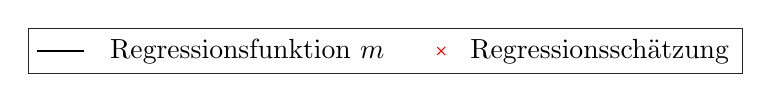
\begin{tikzpicture} 
    \begin{axis}[%
    legend columns=2,
    hide axis,
    xmin=10,
    xmax=50,
    ymin=0,
    ymax=0.4,
    legend style={draw=white!15!black,legend cell align=left,column sep=0.25cm}
    ]
    \addlegendimage{no markers,black}
    \addlegendentry{Regressionsfunktion $m \quad$};
     \addlegendimage{only marks,red,mark=x}
    \addlegendentry{Regressionsschätzung};
    \end{axis}
\end{tikzpicture}}
    \end{subfigure}
     \caption{Approximation der Regressionsfunktion $m(x) = \sin\big(\frac{\pi}{2} \cdot x^2\big)$ durch unseren Neuronale-Netze-Regressionsschätzer mit Parametern $d = 1$, $q = 2$, $R = 10^6$, $a = 3$, $M = 16$ und $N \in \{2,4,8,16\}$.}
    \label{fig:subfig.a.4}
\end{figure}
\begin{figure}
    \begin{subfigure}[b]{0.5\textwidth}
        \centering
        \scalebox{0.9}{
          % This file was created by tikzplotlib v0.9.0.
\begin{tikzpicture}

\begin{axis}[
tick align=outside,
tick pos=left,
title={$N = 2$, $M = 16$},
x grid style={white!69.0196078431373!black},
xmin=-3.34207441715318, xmax=3.35388433148518,
xtick style={color=black},
y grid style={white!69.0196078431373!black},
ymin=\ymin, ymax=\ymax,
ytick style={color=black}
]
\addplot [only marks, mark=x, draw=red, fill=red, colormap/viridis]
table{%
x                      y
2.76238288932011 -0.463161140690246
-2.97867143721344 1.11170632483828
1.34016626636584 0.328103900221429
-2.34602979642214 0.622726053028161
0.262724949982951 0.0932936493533496
0.761496100082008 0.816091744633529
-1.54231724537519 -0.556175431996082
2.48306325147965 -0.206831095835292
0.733875172149707 0.740106936985581
-1.60983185163084 -0.79607432496739
1.62079312559885 -0.801268369711307
-2.36695752001599 0.506958965874763
0.331351911188067 0.172439177397827
-2.43026358118505 0.122820282304857
0.485904436050117 0.348793128272332
-1.48211932367887 -0.26636541363796
0.896800847728478 0.977508873999964
1.29496171714908 0.478516181437511
0.145113687411967 0.0392009166832592
0.945128446218661 0.985127193977801
1.87976307195033 -0.720145744730991
1.84507362985819 -0.821088836712398
0.718091952323177 0.72496250146298
-0.293385227275351 0.133690161783831
-0.552300065715795 0.446007004779764
2.24848571942618 1.10690258854518
1.21759039268623 0.706705010760207
-1.89038986575959 -0.647337063259848
0.39439287977558 0.260129660964836
2.45284819380034 -0.031760800929817
-2.09586004651037 0.547186944572658
2.07310605318424 0.432987962213411
1.9212147978921 -0.42268229011325
-0.00395339221299285 -0.00611598362893603
-2.77449689108578 -0.359048475126319
-2.11498496761839 0.633593665755028
2.53583216813203 -0.578584942642351
-2.73507122380883 -0.591137264797007
-0.765007401567843 0.802265105569046
0.714237808352825 0.702728823520778
-1.8183117665159 -0.893160368520196
2.88647854344178 0.40196424771843
-2.06414860173947 0.391192263526636
0.238075170967647 0.107923152796403
0.708067946079868 0.693809941447383
-1.61406030798178 -0.80237832801808
-0.202146064743951 0.0661752597398166
-0.0539488252024247 0.00467641103052243
1.60117425795925 -0.759221498053604
0.80568451664324 0.883054978089857
-0.194699681607962 0.0657669957348491
1.00165525916385 1.01194312434435
-0.27973544086681 0.132993232649915
0.154269548048458 0.0448735976622029
0.951408249350171 0.97991469529514
-1.91282770827683 -0.494968830008023
1.72829730703384 -0.95265383141678
0.617192025230384 0.542773428611432
2.88199731082397 0.34710537510434
-1.66570083881295 -0.912376899827822
-0.202401155000559 0.0682922335779912
2.37385081559668 0.48990422515938
0.608600458192729 0.529933173808962
1.35575307509289 0.254137742303486
-0.517979014791838 0.402636606867873
1.10585773098792 0.954418295263262
2.67633017908538 -0.956372040261256
-1.79888360556407 -0.930612576634317
1.84419158326392 -0.818575560400849
2.81722807259938 -0.0679580540811622
-2.91258760942001 0.590570951739607
-1.70874248043343 -0.96103507381328
-2.29573847812122 0.903866093881658
1.60454110644872 -0.776723926277638
-2.5127004843436 -0.397618493618822
2.99048135154545 1.1476633703161
-0.662327904724169 0.616087437308203
2.43121659559824 0.0768393232081559
-1.86853437900319 -0.770367755639925
-0.354766801066255 0.189828591452233
2.06887091403722 0.430739557253923
0.571618684039537 0.468378160189806
-0.227051419851858 0.0962063754756209
0.0758984805427056 0.00440032773889413
0.443313161354085 0.29932150950588
-0.358084754486441 0.188772875750377
-1.83864625365714 -0.852579920290961
-2.31620543124488 0.793842041782595
-2.09263243577911 0.532118240625332
-2.6850542168812 -0.861870518303429
0.352058466381789 0.220971405181751
2.08632608421606 0.477348602468043
-0.845283966455336 0.906118498458334
-2.54813476418509 -0.623932706417743
-0.445653528089303 0.290127149013454
0.612047030832008 0.545395976628396
-0.447579206546175 0.31109107137991
1.86432740164422 -0.773626460452391
2.65131747712023 -1.01168670547952
2.21946463961013 1.02986209506946
1.22399698967933 0.715341207285279
-0.178206451306949 0.0586245704236229
1.09618825741951 0.948118498944542
-2.91949013666082 0.64450312547968
2.89486871101226 0.479669686064954
-1.96753600902662 -0.147333755833701
2.43756237577009 0.0856073247905787
1.84265940999664 -0.838022468427495
1.80083810632193 -0.893716240971356
-1.38638365328961 0.147189055446752
-1.68507716545645 -0.939834481817083
-0.427195842515467 0.284818756737455
2.09622660438393 0.529541549093289
-0.297722145169678 0.135173251906132
2.61252068404237 -1.06910605449426
-0.883924036489572 0.945811190170227
0.716352994180558 0.715537304482471
2.88419421813468 0.36779217404373
0.86077513344483 0.929738285328964
-2.72701070375638 -0.628031522435125
-0.218657454289729 0.0799483966696581
-0.991491937718017 1.00055015148373
0.193089291130048 0.0641434561039283
-1.29152274832121 0.485291119828091
-2.26643261861998 1.06097045595707
1.00973393250481 0.993537432134799
1.08815852934784 0.976706533638035
2.20283579999453 0.987892919550483
-2.20571103862358 1.00523980988622
1.79172184966819 -0.911241627435459
1.96061243043077 -0.230791033743328
0.879299614506912 0.946711959907842
-1.7704671253162 -0.958005077057877
-1.43147571356497 -0.0417584295740311
-0.489019094764946 0.35927964111015
0.250794436696388 0.0898393138889789
-0.135372266446698 0.0382754231576303
-0.195240647727783 0.0590833986655301
2.039044261186 0.202943022593416
2.22061419184541 1.01906787645756
1.9005237862606 -0.552821779931867
2.2668085118082 1.00022921431333
0.426052571622439 0.289248182255265
2.78421680003449 -0.278782101155095
0.639266089502806 0.559710312825165
0.623686446478088 0.546320626286095
-1.08421357755229 0.966156657009412
1.08722510470211 0.965170412392293
-2.68820586896783 -0.844143425526716
-2.19272147392835 0.959441060818508
-2.21854699456341 1.04904894369745
0.931207723348414 0.977239534127049
-1.94800444937197 -0.272444504243364
-0.953119060490716 0.981374988096537
-2.73413006500137 -0.59308615160625
-1.59759383930094 -0.753073020888769
2.78534594909577 -0.300131273778273
0.0548364150982064 0.0166918507026227
-2.09355288917141 0.536874786405437
0.138051190406785 0.0295550173370536
2.66105630346648 -1.0106443747517
2.194116084038 0.949641080213007
-0.647604786417679 0.59350062211445
-1.29679490415958 0.472555586334796
1.57037917615645 -0.689148205311893
-1.55709405118147 -0.611196066890769
-1.47460587205589 -0.234138180968196
-2.49548187492042 -0.285234790121326
2.18486456858416 0.911023620109852
-0.312606506278321 0.148741912637024
0.370717563659841 0.225099583267408
1.42026574616112 -0.0121022470556269
1.77893320278717 -0.951438230119911
-0.314951166058117 0.150300460688523
-1.89523466294521 -0.616636045163312
1.97239710916981 -0.124459609744577
-2.81401224103046 -0.104711576452358
2.68036961764771 -0.938675626295439
0.461867078865009 0.312234129758818
2.25233243070412 1.07890743526328
0.651392621841352 0.5903785269043
-1.49004249508606 -0.307677087605436
-1.22322045902457 0.693326609360435
0.197535354189919 0.0799343715089901
2.77246927708256 -0.410877450420673
-1.89302637305893 -0.629590947758836
0.0593902688586541 -0.00156337009736348
-0.937271379378934 0.980221925837238
1.61835206974311 -0.795169607318235
1.81719891859454 -0.850141931932902
-0.4526405381867 0.32138197823583
-1.77526500003398 -0.956024679598113
-2.59746323802687 -0.960521403143004
-1.80811041347663 -0.913497985823252
-1.36559489922371 0.224108649032642
0.592733507455263 0.4999420604217
2.23850098364661 1.07473088392933
-2.23061436692708 1.09110584221959
2.74913245028938 -0.564446119019849
1.09902506312488 0.951038376670626
};
\addplot [semithick, black]
table {%
-3 1
-2.99 0.995576734820054
-2.98 0.982404791977482
-2.97 0.960687140310815
-2.96 0.930698746339696
-2.95 0.892782465918225
-2.94 0.847344438774256
-2.93 0.794849046139829
-2.92 0.735813493407208
-2.91 0.670802080787205
-2.9 0.6004202253259
-2.89 0.525308297382294
-2.88 0.446135333817727
-2.87 0.363592688736647
-2.86 0.278387680690676
-2.85 0.191237292858769
-2.84 0.102861979893671
-2.83 0.0139796319282911
-2.82 -0.0747002572851044
-2.81 -0.162482174923344
-2.8 -0.248689887164819
-2.79 -0.332671415810564
-2.78 -0.413803662790115
-2.77 -0.491496656276015
-2.76000000000001 -0.565197396549224
-2.75000000000001 -0.63439328416361
-2.74000000000001 -0.698615117310616
-2.73000000000001 -0.7574396495474
-2.72000000000001 -0.810491703188593
-2.71000000000001 -0.857445837641644
-2.70000000000001 -0.898027575760592
-2.69000000000001 -0.932014194877928
-2.68000000000001 -0.959235092527838
-2.67000000000001 -0.979571739978357
-2.66000000000001 -0.992957239530362
-2.65000000000001 -0.999375504106505
-2.64000000000001 -0.998860079935072
-2.63000000000001 -0.991492635127341
-2.62000000000001 -0.977401138650261
-2.61000000000001 -0.956757755609883
-2.60000000000001 -0.929776485888277
-2.59000000000001 -0.896710574023413
-2.58000000000001 -0.857849718795458
-2.57000000000001 -0.813517111294285
-2.56000000000001 -0.764066330303094
-2.55000000000001 -0.709878123655345
-2.54000000000001 -0.651357103821107
-2.53000000000001 -0.588928385370132
-2.52000000000001 -0.523034191158988
-2.51000000000001 -0.454130453115695
-2.50000000000001 -0.382683432365167
-2.49000000000001 -0.309166382170306
-2.48000000000001 -0.234056275775223
-2.47000000000001 -0.157830619746354
-2.46000000000001 -0.0809643718325892
-2.45000000000001 -0.00392698072389465
-2.44000000000001 0.072820436603254
-2.43000000000001 0.148827765990005
-2.42000000000001 0.223658403427451
-2.41000000000001 0.296891588141009
-2.40000000000001 0.368124552684589
-2.39000000000001 0.43697448301218
-2.38000000000001 0.503080283168017
-2.37000000000001 0.56610414086275
-2.36000000000001 0.625732891772279
-2.35000000000001 0.681679181898872
-2.34000000000001 0.733682428763456
-2.33000000000001 0.781509583546624
-2.32000000000001 0.824955697558263
-2.31000000000001 0.863844297587357
-2.30000000000001 0.898027575760569
-2.29000000000002 0.927386400518292
-2.28000000000002 0.951830156198068
-2.27000000000002 0.971296419496836
-2.26000000000002 0.985750481765479
-2.25000000000002 0.995184726672186
-2.24000000000002 0.999617873256875
-2.23000000000002 0.999094094789406
-2.22000000000002 0.993682024142277
-2.21000000000002 0.983473656597255
-2.20000000000002 0.96858316112866
-2.19000000000002 0.949145611247931
-2.18000000000002 0.925315646459183
-2.17000000000002 0.897266075268519
-2.16000000000002 0.865186430515806
-2.15000000000002 0.829281487561826
-2.14000000000002 0.789769755571343
-2.13000000000002 0.746881951789148
-2.12000000000002 0.700859468316991
-2.11000000000002 0.651952840469899
-2.10000000000002 0.600420225325985
-2.09000000000002 0.546525898589853
-2.08000000000002 0.490538777371198
-2.07000000000002 0.432730975942088
-2.06000000000002 0.373376400983612
-2.05000000000002 0.31274939226965
-2.04000000000002 0.251123414166708
-2.03000000000002 0.188769802758421
-2.02000000000002 0.125956572835066
-2.01000000000002 0.062947288426061
-2.00000000000002 1.33870012014889e-13
-1.99000000000002 -0.062633749083271
-1.98000000000002 -0.124709844813965
-1.97000000000002 -0.185992451913749
-1.96000000000002 -0.246254789302508
-1.95000000000002 -0.305279831055913
-1.94000000000002 -0.3628609327075
-1.93000000000002 -0.418802383167873
-1.92000000000002 -0.472919882928091
-1.91000000000002 -0.525040949582032
-1.90000000000002 -0.575005252043164
-1.89000000000002 -0.622664875144035
-1.88000000000002 -0.667884516592001
-1.87000000000002 -0.710541618511978
-1.86000000000002 -0.750526436036607
-1.85000000000002 -0.787742045606543
-1.84000000000002 -0.822104295818981
-1.83000000000002 -0.85354170381174
-1.82000000000003 -0.881995300293982
-1.81000000000003 -0.907418426433774
-1.80000000000003 -0.929776485888198
-1.79000000000003 -0.949046655314642
-1.78000000000003 -0.965217556733346
-1.77000000000003 -0.978288895122437
-1.76000000000003 -0.988271064618766
-1.75000000000003 -0.995184726672183
-1.74000000000003 -0.99906036345861
-1.73000000000003 -0.999937809799883
-1.72000000000003 -0.997865766766904
-1.71000000000003 -0.992901300058717
-1.70000000000003 -0.985109326154799
-1.69000000000003 -0.974562089132473
-1.68000000000003 -0.961338630927184
-1.67000000000003 -0.945524257691589
-1.66000000000003 -0.92721000478115
-1.65000000000003 -0.906492102760418
-1.64000000000003 -0.883471446686396
-1.63000000000003 -0.858253070784441
-1.62000000000003 -0.830945630488965
-1.61000000000003 -0.801660893676759
-1.60000000000003 -0.770513242775885
-1.59000000000003 -0.737619189288572
-1.58000000000003 -0.703096902123257
-1.57000000000003 -0.667065750989361
-1.56000000000003 -0.629645865969377
-1.55000000000003 -0.590957714246878
-1.54000000000003 -0.5511216948366
-1.53000000000003 -0.510257752034371
-1.52000000000003 -0.468485008180726
-1.51000000000003 -0.425921416212823
-1.50000000000003 -0.382683432365229
-1.49000000000003 -0.338885709271396
-1.48000000000003 -0.29464080961443
-1.47000000000003 -0.250058940378286
-1.46000000000003 -0.205247707658841
-1.45000000000003 -0.16031189190854
-1.44000000000003 -0.115353243408457
-1.43000000000003 -0.0704702976877775
-1.42000000000003 -0.0257582105426693
-1.41000000000003 0.018691387755514
-1.40000000000003 0.0627905195291638
-1.39000000000003 0.106454968557562
-1.38000000000003 0.149604371296494
-1.37000000000003 0.192162291056312
-1.36000000000003 0.234056275774993
-1.35000000000004 0.275217900052248
-1.34000000000004 0.315582792135412
-1.33000000000004 0.355090646567928
-1.32000000000004 0.393685223226887
-1.31000000000004 0.431314333487567
-1.30000000000004 0.467929814260443
-1.29000000000004 0.503487490649953
-1.28000000000004 0.537947127984647
-1.27000000000004 0.571272373965398
-1.26000000000004 0.603430691672474
-1.25000000000004 0.634393284163532
-1.24000000000004 0.664135011383361
-1.23000000000004 0.692634300092632
-1.22000000000004 0.719873047507249
-1.21000000000004 0.745836519322339
-1.20000000000004 0.770513242775697
-1.19000000000004 0.79389489538482
-1.18000000000004 0.815976189969678
-1.17000000000004 0.836754756550324
-1.16000000000004 0.856231021684473
-1.15000000000004 0.87440808578545
-1.14000000000004 0.891291598935659
-1.13000000000004 0.906889635684947
-1.12000000000004 0.921212569297285
-1.11000000000004 0.93427294588298
-1.10000000000004 0.9460853588275
-1.09000000000004 0.956666323901834
-1.08000000000004 0.966034155413461
-1.07000000000004 0.974208843731348
-1.06000000000004 0.981211934493193
-1.05000000000004 0.987066409778344
-1.04000000000004 0.991796571505593
-1.03000000000004 0.995427927291427
-1.02000000000004 0.997987078981312
-1.01000000000004 0.999501614044331
-1.00000000000004 1
-0.990000000000043 0.999511482025296
-0.980000000000043 0.998065983870084
-0.970000000000043 0.995694012190007
-0.960000000000043 0.992426564387702
-0.950000000000044 0.988295040035889
-0.940000000000044 0.983331155939389
-0.930000000000044 0.977566864877576
-0.920000000000044 0.971034278054095
-0.910000000000045 0.963765591266851
-0.900000000000045 0.955793014798367
-0.890000000000045 0.94714870701456
-0.880000000000045 0.937864711648732
-0.870000000000045 0.927972898737259
-0.860000000000046 0.917504909163832
-0.850000000000046 0.906492102760406
-0.840000000000046 0.894965509904969
-0.830000000000046 0.882955786549018
-0.820000000000046 0.870493172601118
-0.810000000000047 0.857607453587072
-0.800000000000047 0.844327925502078
-0.790000000000047 0.830683362765738
-0.780000000000047 0.816701989186866
-0.770000000000048 0.802411451841723
-0.760000000000048 0.787838797766522
-0.750000000000048 0.773010453362809
-0.740000000000048 0.757952206412552
-0.730000000000048 0.742689190598499
-0.720000000000049 0.727245872424471
-0.710000000000049 0.711646040429847
-0.700000000000049 0.695912796592392
-0.690000000000049 0.68006854981388
-0.680000000000049 0.664135011383549
-0.67000000000005 0.648133192315342
-0.66000000000005 0.632083402456062
-0.65000000000005 0.61600525126299
-0.64000000000005 0.599917650151169
-0.630000000000051 0.583838816312412
-0.620000000000051 0.567786277910133
-0.610000000000051 0.551776880556293
-0.600000000000051 0.535826794979078
-0.590000000000051 0.519951525792427
-0.580000000000052 0.504165921281037
-0.570000000000052 0.488484184117171
-0.560000000000052 0.472919882928293
-0.550000000000052 0.457485964637341
-0.540000000000052 0.442194767500267
-0.530000000000053 0.427058034768333
-0.520000000000053 0.4120869289055
-0.510000000000053 0.397292046294142
-0.500000000000053 0.382683432365167
-0.490000000000054 0.368270597091477
-0.480000000000054 0.354062530786545
-0.470000000000054 0.340067720152659
-0.460000000000054 0.326294164526146
-0.450000000000054 0.312749392269599
-0.440000000000055 0.299440477263786
-0.430000000000055 0.286374055454505
-0.420000000000055 0.273556341412193
-0.410000000000055 0.260993144864562
-0.400000000000055 0.248689887164922
-0.390000000000056 0.23665161766118
-0.380000000000056 0.22488302993274
-0.370000000000056 0.213388477864702
-0.360000000000056 0.202171991530836
-0.350000000000056 0.191237292858801
-0.340000000000057 0.180587811053027
-0.330000000000057 0.170226697752469
-0.320000000000057 0.160156841902239
-0.310000000000057 0.150380884319751
-0.300000000000058 0.140901231937636
-0.290000000000058 0.131720071707145
-0.280000000000058 0.122839384147215
-0.270000000000058 0.114260956525697
-0.260000000000058 0.105986395660502
-0.250000000000059 0.0980171403296064
-0.240000000000059 0.0903544732799798
-0.230000000000059 0.0829995328265039
-0.220000000000059 0.0759533240329385
-0.210000000000059 0.0692167294678623
-0.20000000000006 0.0627905195293508
-0.19000000000006 0.0566753623329036
-0.18000000000006 0.0508718331578319
-0.17000000000006 0.0453804234479493
-0.160000000000061 0.0402015493629836
-0.150000000000061 0.0353355598776498
-0.140000000000061 0.0307827444257893
-0.130000000000061 0.0265433400874004
-0.120000000000061 0.0226175383167529
-0.110000000000062 0.019005491210107
-0.100000000000062 0.0157073173118401
-0.090000000000062 0.012723106958029
-0.0800000000000622 0.0100529271567463
-0.0700000000000625 0.00769682600450373
-0.0600000000000627 0.00565483663842069
-0.0500000000000629 0.00392698072381588
-0.0400000000000631 0.00251327147701166
-0.0300000000000633 0.00141371622321359
-0.0200000000000635 0.000628318489380248
-0.0100000000000637 0.000157079632035528
-6.3948846218409e-14 6.42370078682459e-27
0.00999999999993584 0.00015707963203151
0.0199999999999356 0.000628318489372212
0.0299999999999354 0.00141371622320154
0.0399999999999352 0.00251327147699558
0.049999999999935 0.00392698072379579
0.0599999999999348 0.00565483663839659
0.0699999999999346 0.00769682600447561
0.0799999999999343 0.0100529271567142
0.0899999999999341 0.0127231069579928
0.0999999999999339 0.0157073173117999
0.109999999999934 0.0190054912100628
0.119999999999933 0.0226175383167047
0.129999999999933 0.0265433400873482
0.139999999999933 0.0307827444257331
0.149999999999933 0.0353355598775896
0.159999999999933 0.0402015493629194
0.169999999999932 0.045380423447881
0.179999999999932 0.0508718331577597
0.189999999999932 0.0566753623328273
0.199999999999932 0.0627905195292706
0.209999999999932 0.0692167294677781
0.219999999999931 0.0759533240328503
0.229999999999931 0.0829995328264118
0.239999999999931 0.0903544732798837
0.249999999999931 0.0980171403295065
0.259999999999931 0.105986395660398
0.26999999999993 0.114260956525589
0.27999999999993 0.122839384147103
0.28999999999993 0.131720071707029
0.29999999999993 0.140901231937517
0.309999999999929 0.150380884319628
0.319999999999929 0.160156841902112
0.329999999999929 0.170226697752338
0.339999999999929 0.180587811052893
0.349999999999929 0.191237292858663
0.359999999999928 0.202171991530694
0.369999999999928 0.213388477864557
0.379999999999928 0.224883029932591
0.389999999999928 0.236651617661028
0.399999999999928 0.248689887164767
0.409999999999927 0.260993144864403
0.419999999999927 0.273556341412031
0.429999999999927 0.28637405545434
0.439999999999927 0.299440477263618
0.449999999999926 0.312749392269427
0.459999999999926 0.326294164525971
0.469999999999926 0.340067720152481
0.479999999999926 0.354062530786364
0.489999999999926 0.368270597091294
0.499999999999925 0.382683432364981
0.509999999999925 0.397292046293954
0.519999999999925 0.412086928905309
0.529999999999925 0.42705803476814
0.539999999999925 0.442194767500072
0.549999999999924 0.457485964637144
0.559999999999924 0.472919882928095
0.569999999999924 0.488484184116971
0.579999999999924 0.504165921280836
0.589999999999923 0.519951525792225
0.599999999999923 0.535826794978874
0.609999999999923 0.551776880556088
0.619999999999923 0.567786277909928
0.629999999999923 0.583838816312206
0.639999999999922 0.599917650150963
0.649999999999922 0.616005251262785
0.659999999999922 0.632083402455857
0.669999999999922 0.648133192315137
0.679999999999922 0.664135011383345
0.689999999999921 0.680068549813677
0.699999999999921 0.69591279659219
0.709999999999921 0.711646040429646
0.719999999999921 0.727245872424273
0.72999999999992 0.742689190598303
0.73999999999992 0.757952206412358
0.74999999999992 0.773010453362617
0.75999999999992 0.787838797766334
0.76999999999992 0.802411451841539
0.779999999999919 0.816701989186685
0.789999999999919 0.830683362765561
0.799999999999919 0.844327925501906
0.809999999999919 0.857607453586905
0.819999999999919 0.870493172600956
0.829999999999918 0.882955786548861
0.839999999999918 0.894965509904818
0.849999999999918 0.906492102760262
0.859999999999918 0.917504909163694
0.869999999999918 0.927972898737128
0.879999999999917 0.93786471164861
0.889999999999917 0.947148707014445
0.899999999999917 0.955793014798261
0.909999999999917 0.963765591266753
0.919999999999916 0.971034278054007
0.929999999999916 0.977566864877497
0.939999999999916 0.98333115593932
0.949999999999916 0.988295040035831
0.959999999999916 0.992426564387655
0.969999999999915 0.995694012189971
0.979999999999915 0.99806598387006
0.989999999999915 0.999511482025283
0.999999999999915 1
1.00999999999991 0.999501614044344
1.01999999999991 0.997987078981338
1.02999999999991 0.995427927291467
1.03999999999991 0.991796571505646
1.04999999999991 0.987066409778411
1.05999999999991 0.981211934493276
1.06999999999991 0.974208843731445
1.07999999999991 0.966034155413573
1.08999999999991 0.956666323901962
1.09999999999991 0.946085358827643
1.10999999999991 0.934272945883139
1.11999999999991 0.92121256929746
1.12999999999991 0.906889635685138
1.13999999999991 0.891291598935866
1.14999999999991 0.874408085785674
1.15999999999991 0.856231021684713
1.16999999999991 0.836754756550582
1.17999999999991 0.815976189969952
1.18999999999991 0.793894895385111
1.19999999999991 0.770513242776004
1.20999999999991 0.745836519322663
1.21999999999991 0.719873047507589
1.22999999999991 0.692634300092988
1.23999999999991 0.664135011383733
1.24999999999991 0.63439328416392
1.25999999999991 0.603430691672878
1.26999999999991 0.571272373965817
1.27999999999991 0.537947127985081
1.28999999999991 0.503487490650401
1.29999999999991 0.467929814260904
1.30999999999991 0.431314333488042
1.31999999999991 0.393685223227375
1.32999999999991 0.355090646568427
1.33999999999991 0.315582792135923
1.34999999999991 0.27521790005277
1.35999999999991 0.234056275775525
1.36999999999991 0.192162291056853
1.37999999999991 0.149604371297043
1.38999999999991 0.106454968558117
1.39999999999991 0.0627905195297253
1.40999999999991 0.0186913877560805
1.41999999999991 -0.0257582105420993
1.42999999999991 -0.0704702976872039
1.43999999999991 -0.115353243407883
1.44999999999991 -0.160311891907964
1.4599999999999 -0.205247707658268
1.4699999999999 -0.250058940377715
1.4799999999999 -0.294640809613862
1.4899999999999 -0.338885709270833
1.4999999999999 -0.382683432364672
1.5099999999999 -0.425921416212274
1.5199999999999 -0.468485008180186
1.5299999999999 -0.510257752033843
1.5399999999999 -0.551121694836084
1.5499999999999 -0.590957714246376
1.5599999999999 -0.62964586596889
1.5699999999999 -0.667065750988891
1.5799999999999 -0.703096902122806
1.5899999999999 -0.73761918928814
1.5999999999999 -0.770513242775475
1.6099999999999 -0.801660893676373
1.6199999999999 -0.830945630488602
1.6299999999999 -0.858253070784105
1.6399999999999 -0.883471446686087
1.6499999999999 -0.906492102760138
1.6599999999999 -0.9272100047809
1.6699999999999 -0.945524257691371
1.6799999999999 -0.961338630926998
1.6899999999999 -0.974562089132321
1.6999999999999 -0.985109326154682
1.7099999999999 -0.992901300058635
1.7199999999999 -0.997865766766859
1.7299999999999 -0.999937809799876
1.7399999999999 -0.99906036345864
1.7499999999999 -0.995184726672251
1.7599999999999 -0.988271064618874
1.7699999999999 -0.978288895122584
1.7799999999999 -0.965217556733533
1.7899999999999 -0.949046655314868
1.7999999999999 -0.929776485888465
1.8099999999999 -0.90741842643408
1.8199999999999 -0.881995300294327
1.8299999999999 -0.853541703812123
1.8399999999999 -0.822104295819402
1.8499999999999 -0.787742045607001
1.8599999999999 -0.750526436037101
1.8699999999999 -0.710541618512508
1.8799999999999 -0.667884516592564
1.8899999999999 -0.622664875144629
1.8999999999999 -0.575005252043788
1.9099999999999 -0.525040949582685
1.9199999999999 -0.47291988292877
1.92999999999989 -0.418802383168577
1.93999999999989 -0.362860932708227
1.94999999999989 -0.305279831056659
1.95999999999989 -0.246254789303272
1.96999999999989 -0.185992451914526
1.97999999999989 -0.124709844814754
1.98999999999989 -0.0626337490840697
1.99999999999989 -6.69931457813724e-13
2.00999999999989 0.0629472884252544
2.01999999999989 0.12595657283426
2.02999999999989 0.18876980275762
2.03999999999989 0.251123414165916
2.04999999999989 0.312749392268867
2.05999999999989 0.373376400982844
2.06999999999989 0.432730975941339
2.07999999999989 0.490538777370471
2.08999999999989 0.54652589858915
2.09999999999989 0.600420225325311
2.10999999999989 0.651952840469257
2.11999999999989 0.700859468316383
2.12999999999989 0.746881951788579
2.13999999999989 0.789769755570817
2.14999999999989 0.829281487561343
2.15999999999989 0.865186430515371
2.16999999999989 0.897266075268134
2.17999999999989 0.925315646458851
2.18999999999989 0.949145611247653
2.19999999999989 0.968583161128441
2.20999999999989 0.983473656597094
2.21999999999989 0.993682024142177
2.22999999999989 0.999094094789368
2.23999999999989 0.9996178732569
2.24999999999989 0.995184726672274
2.25999999999989 0.985750481765632
2.26999999999989 0.971296419497053
2.27999999999989 0.951830156198348
2.28999999999989 0.927386400518636
2.29999999999989 0.898027575760974
2.30999999999989 0.863844297587825
2.31999999999989 0.82495569755879
2.32999999999989 0.781509583547208
2.33999999999989 0.733682428764095
2.34999999999989 0.681679181899562
2.35999999999989 0.625732891773019
2.36999999999989 0.566104140863535
2.37999999999989 0.503080283168843
2.38999999999989 0.436974483013044
2.39999999999988 0.368124552685486
2.40999999999988 0.296891588141934
2.41999999999988 0.2236584034284
2.42999999999988 0.148827765990971
2.43999999999988 0.072820436604232
2.44999999999988 -0.00392698072291233
2.45999999999988 -0.0809643718316048
2.46999999999988 -0.157830619745374
2.47999999999988 -0.234056275774253
2.48999999999988 -0.309166382169355
2.49999999999988 -0.382683432364238
2.50999999999988 -0.454130453114798
2.51999999999988 -0.523034191158123
2.52999999999988 -0.58892838536931
2.53999999999988 -0.651357103820333
2.54999999999988 -0.709878123654623
2.55999999999988 -0.764066330302429
2.56999999999988 -0.813517111293685
2.57999999999988 -0.857849718794925
2.58999999999988 -0.896710574022952
2.59999999999988 -0.929776485887892
2.60999999999988 -0.956757755609577
2.61999999999988 -0.977401138650039
2.62999999999988 -0.991492635127203
2.63999999999988 -0.998860079935021
2.64999999999988 -0.999375504106543
2.65999999999988 -0.992957239530489
2.66999999999988 -0.979571739978573
2.67999999999988 -0.959235092528142
2.68999999999988 -0.93201419487832
2.69999999999988 -0.898027575761069
2.70999999999988 -0.857445837642205
2.71999999999988 -0.810491703189233
2.72999999999988 -0.757439649548115
2.73999999999988 -0.698615117311402
2.74999999999988 -0.634393284164464
2.75999999999988 -0.565197396550139
2.76999999999988 -0.491496656276984
2.77999999999988 -0.413803662791132
2.78999999999988 -0.332671415811622
2.79999999999988 -0.248689887165909
2.80999999999988 -0.162482174924459
2.81999999999988 -0.0747002572862345
2.82999999999988 0.0139796319271562
2.83999999999988 0.102861979892536
2.84999999999988 0.191237292857646
2.85999999999988 0.278387680689572
2.86999999999987 0.36359268873557
2.87999999999987 0.44613533381669
2.88999999999987 0.525308297381304
2.89999999999987 0.600420225324967
2.90999999999987 0.670802080786339
2.91999999999987 0.735813493406414
2.92999999999987 0.794849046139114
2.93999999999987 0.847344438773628
2.94999999999987 0.892782465917691
2.95999999999987 0.930698746339261
2.96999999999987 0.960687140310484
2.97999999999987 0.982404791977258
2.98999999999987 0.995576734819941
};
\end{axis}

\end{tikzpicture}
}
          \label{test2}
    \end{subfigure}
    \begin{subfigure}[b]{0.5\textwidth}
    \centering
    \scalebox{0.9}{
           % This file was created by tikzplotlib v0.9.0.
\begin{tikzpicture}

\begin{axis}[
tick align=outside,
tick pos=left,
title={$N = 4$, $M = 9$},
x grid style={white!69.0196078431373!black},
xmin=-3.34207441715318, xmax=3.35388433148518,
xtick style={color=black},
y grid style={white!69.0196078431373!black},
ymin=\ymin, ymax=\ymax,
ytick style={color=black}
]
\addplot [only marks, mark=x, draw=red, fill=red, colormap/viridis]
table{%
x                      y
2.76238288932011 -0.517095249307967
-2.97867143721344 1.37061814914596
1.34016626636584 0.472377538424305
-2.34602979642214 0.752116061084845
0.262724949982951 0.120767416328344
0.761496100082008 0.822733431300647
-1.54231724537519 -0.543570008860521
2.48306325147965 -0.277499297454561
0.733875172149707 0.748224504109002
-1.60983185163084 -0.896484455897655
1.62079312559885 -0.861526093493598
-2.36695752001599 0.610030733667231
0.331351911188067 0.236583910439349
-2.43026358118505 0.137706236366698
0.485904436050117 0.425143232003497
-1.48211932367887 -0.244608149775098
0.896800847728478 0.988562584870182
1.29496171714908 0.413534101156168
0.145113687411967 0.0427639496337842
0.945128446218661 1.01101782990031
1.87976307195033 -0.616412322487849
1.84507362985819 -0.73948190291735
0.718091952323177 0.678508707555179
-0.293385227275351 0.122115896438473
-0.552300065715795 0.473563498833174
2.24848571942618 0.96980394904679
1.21759039268623 0.735131061388096
-1.89038986575959 -0.433997064505982
0.39439287977558 0.23994330433402
2.45284819380034 -0.110954655304946
-2.09586004651037 0.479337077008519
2.07310605318424 0.411108080574449
1.9212147978921 -0.330299481899987
-0.00395339221299285 0.0798707072496855
-2.77449689108578 -0.520720037018834
-2.11498496761839 0.573926962866648
2.53583216813203 -0.684400371146222
-2.73507122380883 -0.658859760944423
-0.765007401567843 0.807638415374486
0.714237808352825 0.71053619383886
-1.8183117665159 -0.732998911614185
2.88647854344178 0.197543121993093
-2.06414860173947 0.34545901707234
0.238075170967647 0.0314363601274662
0.708067946079868 0.770243510797042
-1.61406030798178 -0.902480022891297
-0.202146064743951 0.0398159633290017
-0.0539488252024247 0.0827682358240614
1.60117425795925 -0.838598684603757
0.80568451664324 0.797591099153452
-0.194699681607962 0.0458691620939335
1.00165525916385 0.975587362011215
-0.27973544086681 0.102926796578904
0.154269548048458 0.0750774675650994
0.951408249350171 0.96817354830566
-1.91282770827683 -0.320623384751374
1.72829730703384 -1.02872841542274
0.617192025230384 0.593223474523237
2.88199731082397 0.250674935825301
-1.66570083881295 -1.19219884787885
-0.202401155000559 0.105344271625217
2.37385081559668 0.511221279409992
0.608600458192729 0.534231871595205
1.35575307509289 0.158514801507645
-0.517979014791838 0.404952085362249
1.10585773098792 0.944185181168384
2.67633017908538 -0.868248969817628
-1.79888360556407 -0.80951884948892
1.84419158326392 -0.662872543308299
2.81722807259938 -0.195910958466151
-2.91258760942001 0.508235330829329
-1.70874248043343 -1.11233897663238
-2.29573847812122 0.883921535963352
1.60454110644872 -0.833984157216494
-2.5127004843436 -0.329510450422096
2.99048135154545 1.4347682229741
-0.662327904724169 0.622300719369605
2.43121659559824 0.0536608801501041
-1.86853437900319 -0.512921909109836
-0.354766801066255 0.129524277218901
2.06887091403722 0.4093443744687
0.571618684039537 0.528162101110831
-0.227051419851858 0.103107920821338
0.0758984805427056 0.0596464971600453
0.443313161354085 0.311205270429855
-0.358084754486441 0.151926219101392
-1.83864625365714 -0.630267086055063
-2.31620543124488 0.881517341557598
-2.09263243577911 0.466479919403559
-2.6850542168812 -0.739377211048862
0.352058466381789 0.222544120819151
2.08632608421606 0.41217052873169
-0.845283966455336 0.877607637851162
-2.54813476418509 -0.498688554563954
-0.445653528089303 0.277785075176291
0.612047030832008 0.559374437524647
-0.447579206546175 0.303416572251721
1.86432740164422 -0.688287890549278
2.65131747712023 -0.782787058658197
2.21946463961013 0.97891867694362
1.22399698967933 0.644460951074003
-0.178206451306949 0.0847064263135998
1.09618825741951 0.921466089166719
-2.91949013666082 0.572706439131069
2.89486871101226 0.319081324507739
-1.96753600902662 -0.0556643704125329
2.43756237577009 -0.046613776644945
1.84265940999664 -0.800864172052358
1.80083810632193 -0.797839569448004
-1.38638365328961 0.174286737093842
-1.68507716545645 -1.1457072195658
-0.427195842515467 0.256869100826428
2.09622660438393 0.384459115582955
-0.297722145169678 0.0889364877393498
2.61252068404237 -0.702980907266519
-0.883924036489572 0.91811390748038
0.716352994180558 0.703791663645502
2.88419421813468 0.210117772070745
0.86077513344483 0.871191369908247
-2.72701070375638 -0.682164581508055
-0.218657454289729 0.0974697329508443
-0.991491937718017 1.01251477647784
0.193089291130048 0.0538154209691093
-1.29152274832121 0.51114310688388
-2.26643261861998 0.862622232674629
1.00973393250481 1.07521233138725
1.08815852934784 0.986741962826321
2.20283579999453 0.965419765552822
-2.20571103862358 0.809497499163095
1.79172184966819 -0.991185850741632
1.96061243043077 -0.184944785469812
0.879299614506912 0.917239166159193
-1.7704671253162 -0.92028003333676
-1.43147571356497 -0.0252198979909884
-0.489019094764946 0.340379529401216
0.250794436696388 0.0744947437740209
-0.135372266446698 0.00961039925229678
-0.195240647727783 0.0442512797228618
2.039044261186 0.252434278932765
2.22061419184541 0.980403470307336
1.9005237862606 -0.43566314537627
2.2668085118082 1.00474161230843
0.426052571622439 0.235320740430228
2.78421680003449 -0.490009258661558
0.639266089502806 0.62304849523063
0.623686446478088 0.537071387417394
-1.08421357755229 0.9571373339504
1.08722510470211 1.02286231941429
-2.68820586896783 -0.728134554110707
-2.19272147392835 0.780698967596735
-2.21854699456341 0.839928481597721
0.931207723348414 0.997703854583266
-1.94800444937197 -0.159860940725491
-0.953119060490716 0.99366066810153
-2.73413006500137 -0.657233308344879
-1.59759383930094 -0.807450726892544
2.78534594909577 -0.439271347569913
0.0548364150982064 0.0410734151900478
-2.09355288917141 0.481316279859282
0.138051190406785 0.0325159928676616
2.66105630346648 -0.952222556080768
2.194116084038 0.952846321938394
-0.647604786417679 0.615992088537527
-1.29679490415958 0.500734323403926
1.57037917615645 -0.724855034372997
-1.55709405118147 -0.611043305657295
-1.47460587205589 -0.192250704085788
-2.49548187492042 -0.236022051454879
2.18486456858416 0.878138820593733
-0.312606506278321 0.15103489523274
0.370717563659841 0.180309963784226
1.42026574616112 -0.00681625333992493
1.77893320278717 -0.974578717945337
-0.314951166058117 0.124554331449597
-1.89523466294521 -0.401513706090525
1.97239710916981 -0.111021157507268
-2.81401224103046 -0.306303066428906
2.68036961764771 -0.825522021650802
0.461867078865009 0.344822252453656
2.25233243070412 1.03189154265088
0.651392621841352 0.658016287698185
-1.49004249508606 -0.297609508233063
-1.22322045902457 0.700742534472009
0.197535354189919 0.0538267305009223
2.77246927708256 -0.473261002976371
-1.89302637305893 -0.400281269257716
0.0593902688586541 -0.000447585719847817
-0.937271379378934 0.970397238890148
1.61835206974311 -0.829931788043143
1.81719891859454 -0.886291797545599
-0.4526405381867 0.296072001239353
-1.77526500003398 -0.884620062901837
-2.59746323802687 -0.65054488987353
-1.80811041347663 -0.783697345600194
-1.36559489922371 0.242253178454142
0.592733507455263 0.538965388915579
2.23850098364661 1.08266311731778
-2.23061436692708 0.860756978807439
2.74913245028938 -0.3965951637636
1.09902506312488 1.00552228510154
};
\addplot [semithick, black]
table {%
-3 1
-2.99 0.995576734820054
-2.98 0.982404791977482
-2.97 0.960687140310815
-2.96 0.930698746339696
-2.95 0.892782465918225
-2.94 0.847344438774256
-2.93 0.794849046139829
-2.92 0.735813493407208
-2.91 0.670802080787205
-2.9 0.6004202253259
-2.89 0.525308297382294
-2.88 0.446135333817727
-2.87 0.363592688736647
-2.86 0.278387680690676
-2.85 0.191237292858769
-2.84 0.102861979893671
-2.83 0.0139796319282911
-2.82 -0.0747002572851044
-2.81 -0.162482174923344
-2.8 -0.248689887164819
-2.79 -0.332671415810564
-2.78 -0.413803662790115
-2.77 -0.491496656276015
-2.76000000000001 -0.565197396549224
-2.75000000000001 -0.63439328416361
-2.74000000000001 -0.698615117310616
-2.73000000000001 -0.7574396495474
-2.72000000000001 -0.810491703188593
-2.71000000000001 -0.857445837641644
-2.70000000000001 -0.898027575760592
-2.69000000000001 -0.932014194877928
-2.68000000000001 -0.959235092527838
-2.67000000000001 -0.979571739978357
-2.66000000000001 -0.992957239530362
-2.65000000000001 -0.999375504106505
-2.64000000000001 -0.998860079935072
-2.63000000000001 -0.991492635127341
-2.62000000000001 -0.977401138650261
-2.61000000000001 -0.956757755609883
-2.60000000000001 -0.929776485888277
-2.59000000000001 -0.896710574023413
-2.58000000000001 -0.857849718795458
-2.57000000000001 -0.813517111294285
-2.56000000000001 -0.764066330303094
-2.55000000000001 -0.709878123655345
-2.54000000000001 -0.651357103821107
-2.53000000000001 -0.588928385370132
-2.52000000000001 -0.523034191158988
-2.51000000000001 -0.454130453115695
-2.50000000000001 -0.382683432365167
-2.49000000000001 -0.309166382170306
-2.48000000000001 -0.234056275775223
-2.47000000000001 -0.157830619746354
-2.46000000000001 -0.0809643718325892
-2.45000000000001 -0.00392698072389465
-2.44000000000001 0.072820436603254
-2.43000000000001 0.148827765990005
-2.42000000000001 0.223658403427451
-2.41000000000001 0.296891588141009
-2.40000000000001 0.368124552684589
-2.39000000000001 0.43697448301218
-2.38000000000001 0.503080283168017
-2.37000000000001 0.56610414086275
-2.36000000000001 0.625732891772279
-2.35000000000001 0.681679181898872
-2.34000000000001 0.733682428763456
-2.33000000000001 0.781509583546624
-2.32000000000001 0.824955697558263
-2.31000000000001 0.863844297587357
-2.30000000000001 0.898027575760569
-2.29000000000002 0.927386400518292
-2.28000000000002 0.951830156198068
-2.27000000000002 0.971296419496836
-2.26000000000002 0.985750481765479
-2.25000000000002 0.995184726672186
-2.24000000000002 0.999617873256875
-2.23000000000002 0.999094094789406
-2.22000000000002 0.993682024142277
-2.21000000000002 0.983473656597255
-2.20000000000002 0.96858316112866
-2.19000000000002 0.949145611247931
-2.18000000000002 0.925315646459183
-2.17000000000002 0.897266075268519
-2.16000000000002 0.865186430515806
-2.15000000000002 0.829281487561826
-2.14000000000002 0.789769755571343
-2.13000000000002 0.746881951789148
-2.12000000000002 0.700859468316991
-2.11000000000002 0.651952840469899
-2.10000000000002 0.600420225325985
-2.09000000000002 0.546525898589853
-2.08000000000002 0.490538777371198
-2.07000000000002 0.432730975942088
-2.06000000000002 0.373376400983612
-2.05000000000002 0.31274939226965
-2.04000000000002 0.251123414166708
-2.03000000000002 0.188769802758421
-2.02000000000002 0.125956572835066
-2.01000000000002 0.062947288426061
-2.00000000000002 1.33870012014889e-13
-1.99000000000002 -0.062633749083271
-1.98000000000002 -0.124709844813965
-1.97000000000002 -0.185992451913749
-1.96000000000002 -0.246254789302508
-1.95000000000002 -0.305279831055913
-1.94000000000002 -0.3628609327075
-1.93000000000002 -0.418802383167873
-1.92000000000002 -0.472919882928091
-1.91000000000002 -0.525040949582032
-1.90000000000002 -0.575005252043164
-1.89000000000002 -0.622664875144035
-1.88000000000002 -0.667884516592001
-1.87000000000002 -0.710541618511978
-1.86000000000002 -0.750526436036607
-1.85000000000002 -0.787742045606543
-1.84000000000002 -0.822104295818981
-1.83000000000002 -0.85354170381174
-1.82000000000003 -0.881995300293982
-1.81000000000003 -0.907418426433774
-1.80000000000003 -0.929776485888198
-1.79000000000003 -0.949046655314642
-1.78000000000003 -0.965217556733346
-1.77000000000003 -0.978288895122437
-1.76000000000003 -0.988271064618766
-1.75000000000003 -0.995184726672183
-1.74000000000003 -0.99906036345861
-1.73000000000003 -0.999937809799883
-1.72000000000003 -0.997865766766904
-1.71000000000003 -0.992901300058717
-1.70000000000003 -0.985109326154799
-1.69000000000003 -0.974562089132473
-1.68000000000003 -0.961338630927184
-1.67000000000003 -0.945524257691589
-1.66000000000003 -0.92721000478115
-1.65000000000003 -0.906492102760418
-1.64000000000003 -0.883471446686396
-1.63000000000003 -0.858253070784441
-1.62000000000003 -0.830945630488965
-1.61000000000003 -0.801660893676759
-1.60000000000003 -0.770513242775885
-1.59000000000003 -0.737619189288572
-1.58000000000003 -0.703096902123257
-1.57000000000003 -0.667065750989361
-1.56000000000003 -0.629645865969377
-1.55000000000003 -0.590957714246878
-1.54000000000003 -0.5511216948366
-1.53000000000003 -0.510257752034371
-1.52000000000003 -0.468485008180726
-1.51000000000003 -0.425921416212823
-1.50000000000003 -0.382683432365229
-1.49000000000003 -0.338885709271396
-1.48000000000003 -0.29464080961443
-1.47000000000003 -0.250058940378286
-1.46000000000003 -0.205247707658841
-1.45000000000003 -0.16031189190854
-1.44000000000003 -0.115353243408457
-1.43000000000003 -0.0704702976877775
-1.42000000000003 -0.0257582105426693
-1.41000000000003 0.018691387755514
-1.40000000000003 0.0627905195291638
-1.39000000000003 0.106454968557562
-1.38000000000003 0.149604371296494
-1.37000000000003 0.192162291056312
-1.36000000000003 0.234056275774993
-1.35000000000004 0.275217900052248
-1.34000000000004 0.315582792135412
-1.33000000000004 0.355090646567928
-1.32000000000004 0.393685223226887
-1.31000000000004 0.431314333487567
-1.30000000000004 0.467929814260443
-1.29000000000004 0.503487490649953
-1.28000000000004 0.537947127984647
-1.27000000000004 0.571272373965398
-1.26000000000004 0.603430691672474
-1.25000000000004 0.634393284163532
-1.24000000000004 0.664135011383361
-1.23000000000004 0.692634300092632
-1.22000000000004 0.719873047507249
-1.21000000000004 0.745836519322339
-1.20000000000004 0.770513242775697
-1.19000000000004 0.79389489538482
-1.18000000000004 0.815976189969678
-1.17000000000004 0.836754756550324
-1.16000000000004 0.856231021684473
-1.15000000000004 0.87440808578545
-1.14000000000004 0.891291598935659
-1.13000000000004 0.906889635684947
-1.12000000000004 0.921212569297285
-1.11000000000004 0.93427294588298
-1.10000000000004 0.9460853588275
-1.09000000000004 0.956666323901834
-1.08000000000004 0.966034155413461
-1.07000000000004 0.974208843731348
-1.06000000000004 0.981211934493193
-1.05000000000004 0.987066409778344
-1.04000000000004 0.991796571505593
-1.03000000000004 0.995427927291427
-1.02000000000004 0.997987078981312
-1.01000000000004 0.999501614044331
-1.00000000000004 1
-0.990000000000043 0.999511482025296
-0.980000000000043 0.998065983870084
-0.970000000000043 0.995694012190007
-0.960000000000043 0.992426564387702
-0.950000000000044 0.988295040035889
-0.940000000000044 0.983331155939389
-0.930000000000044 0.977566864877576
-0.920000000000044 0.971034278054095
-0.910000000000045 0.963765591266851
-0.900000000000045 0.955793014798367
-0.890000000000045 0.94714870701456
-0.880000000000045 0.937864711648732
-0.870000000000045 0.927972898737259
-0.860000000000046 0.917504909163832
-0.850000000000046 0.906492102760406
-0.840000000000046 0.894965509904969
-0.830000000000046 0.882955786549018
-0.820000000000046 0.870493172601118
-0.810000000000047 0.857607453587072
-0.800000000000047 0.844327925502078
-0.790000000000047 0.830683362765738
-0.780000000000047 0.816701989186866
-0.770000000000048 0.802411451841723
-0.760000000000048 0.787838797766522
-0.750000000000048 0.773010453362809
-0.740000000000048 0.757952206412552
-0.730000000000048 0.742689190598499
-0.720000000000049 0.727245872424471
-0.710000000000049 0.711646040429847
-0.700000000000049 0.695912796592392
-0.690000000000049 0.68006854981388
-0.680000000000049 0.664135011383549
-0.67000000000005 0.648133192315342
-0.66000000000005 0.632083402456062
-0.65000000000005 0.61600525126299
-0.64000000000005 0.599917650151169
-0.630000000000051 0.583838816312412
-0.620000000000051 0.567786277910133
-0.610000000000051 0.551776880556293
-0.600000000000051 0.535826794979078
-0.590000000000051 0.519951525792427
-0.580000000000052 0.504165921281037
-0.570000000000052 0.488484184117171
-0.560000000000052 0.472919882928293
-0.550000000000052 0.457485964637341
-0.540000000000052 0.442194767500267
-0.530000000000053 0.427058034768333
-0.520000000000053 0.4120869289055
-0.510000000000053 0.397292046294142
-0.500000000000053 0.382683432365167
-0.490000000000054 0.368270597091477
-0.480000000000054 0.354062530786545
-0.470000000000054 0.340067720152659
-0.460000000000054 0.326294164526146
-0.450000000000054 0.312749392269599
-0.440000000000055 0.299440477263786
-0.430000000000055 0.286374055454505
-0.420000000000055 0.273556341412193
-0.410000000000055 0.260993144864562
-0.400000000000055 0.248689887164922
-0.390000000000056 0.23665161766118
-0.380000000000056 0.22488302993274
-0.370000000000056 0.213388477864702
-0.360000000000056 0.202171991530836
-0.350000000000056 0.191237292858801
-0.340000000000057 0.180587811053027
-0.330000000000057 0.170226697752469
-0.320000000000057 0.160156841902239
-0.310000000000057 0.150380884319751
-0.300000000000058 0.140901231937636
-0.290000000000058 0.131720071707145
-0.280000000000058 0.122839384147215
-0.270000000000058 0.114260956525697
-0.260000000000058 0.105986395660502
-0.250000000000059 0.0980171403296064
-0.240000000000059 0.0903544732799798
-0.230000000000059 0.0829995328265039
-0.220000000000059 0.0759533240329385
-0.210000000000059 0.0692167294678623
-0.20000000000006 0.0627905195293508
-0.19000000000006 0.0566753623329036
-0.18000000000006 0.0508718331578319
-0.17000000000006 0.0453804234479493
-0.160000000000061 0.0402015493629836
-0.150000000000061 0.0353355598776498
-0.140000000000061 0.0307827444257893
-0.130000000000061 0.0265433400874004
-0.120000000000061 0.0226175383167529
-0.110000000000062 0.019005491210107
-0.100000000000062 0.0157073173118401
-0.090000000000062 0.012723106958029
-0.0800000000000622 0.0100529271567463
-0.0700000000000625 0.00769682600450373
-0.0600000000000627 0.00565483663842069
-0.0500000000000629 0.00392698072381588
-0.0400000000000631 0.00251327147701166
-0.0300000000000633 0.00141371622321359
-0.0200000000000635 0.000628318489380248
-0.0100000000000637 0.000157079632035528
-6.3948846218409e-14 6.42370078682459e-27
0.00999999999993584 0.00015707963203151
0.0199999999999356 0.000628318489372212
0.0299999999999354 0.00141371622320154
0.0399999999999352 0.00251327147699558
0.049999999999935 0.00392698072379579
0.0599999999999348 0.00565483663839659
0.0699999999999346 0.00769682600447561
0.0799999999999343 0.0100529271567142
0.0899999999999341 0.0127231069579928
0.0999999999999339 0.0157073173117999
0.109999999999934 0.0190054912100628
0.119999999999933 0.0226175383167047
0.129999999999933 0.0265433400873482
0.139999999999933 0.0307827444257331
0.149999999999933 0.0353355598775896
0.159999999999933 0.0402015493629194
0.169999999999932 0.045380423447881
0.179999999999932 0.0508718331577597
0.189999999999932 0.0566753623328273
0.199999999999932 0.0627905195292706
0.209999999999932 0.0692167294677781
0.219999999999931 0.0759533240328503
0.229999999999931 0.0829995328264118
0.239999999999931 0.0903544732798837
0.249999999999931 0.0980171403295065
0.259999999999931 0.105986395660398
0.26999999999993 0.114260956525589
0.27999999999993 0.122839384147103
0.28999999999993 0.131720071707029
0.29999999999993 0.140901231937517
0.309999999999929 0.150380884319628
0.319999999999929 0.160156841902112
0.329999999999929 0.170226697752338
0.339999999999929 0.180587811052893
0.349999999999929 0.191237292858663
0.359999999999928 0.202171991530694
0.369999999999928 0.213388477864557
0.379999999999928 0.224883029932591
0.389999999999928 0.236651617661028
0.399999999999928 0.248689887164767
0.409999999999927 0.260993144864403
0.419999999999927 0.273556341412031
0.429999999999927 0.28637405545434
0.439999999999927 0.299440477263618
0.449999999999926 0.312749392269427
0.459999999999926 0.326294164525971
0.469999999999926 0.340067720152481
0.479999999999926 0.354062530786364
0.489999999999926 0.368270597091294
0.499999999999925 0.382683432364981
0.509999999999925 0.397292046293954
0.519999999999925 0.412086928905309
0.529999999999925 0.42705803476814
0.539999999999925 0.442194767500072
0.549999999999924 0.457485964637144
0.559999999999924 0.472919882928095
0.569999999999924 0.488484184116971
0.579999999999924 0.504165921280836
0.589999999999923 0.519951525792225
0.599999999999923 0.535826794978874
0.609999999999923 0.551776880556088
0.619999999999923 0.567786277909928
0.629999999999923 0.583838816312206
0.639999999999922 0.599917650150963
0.649999999999922 0.616005251262785
0.659999999999922 0.632083402455857
0.669999999999922 0.648133192315137
0.679999999999922 0.664135011383345
0.689999999999921 0.680068549813677
0.699999999999921 0.69591279659219
0.709999999999921 0.711646040429646
0.719999999999921 0.727245872424273
0.72999999999992 0.742689190598303
0.73999999999992 0.757952206412358
0.74999999999992 0.773010453362617
0.75999999999992 0.787838797766334
0.76999999999992 0.802411451841539
0.779999999999919 0.816701989186685
0.789999999999919 0.830683362765561
0.799999999999919 0.844327925501906
0.809999999999919 0.857607453586905
0.819999999999919 0.870493172600956
0.829999999999918 0.882955786548861
0.839999999999918 0.894965509904818
0.849999999999918 0.906492102760262
0.859999999999918 0.917504909163694
0.869999999999918 0.927972898737128
0.879999999999917 0.93786471164861
0.889999999999917 0.947148707014445
0.899999999999917 0.955793014798261
0.909999999999917 0.963765591266753
0.919999999999916 0.971034278054007
0.929999999999916 0.977566864877497
0.939999999999916 0.98333115593932
0.949999999999916 0.988295040035831
0.959999999999916 0.992426564387655
0.969999999999915 0.995694012189971
0.979999999999915 0.99806598387006
0.989999999999915 0.999511482025283
0.999999999999915 1
1.00999999999991 0.999501614044344
1.01999999999991 0.997987078981338
1.02999999999991 0.995427927291467
1.03999999999991 0.991796571505646
1.04999999999991 0.987066409778411
1.05999999999991 0.981211934493276
1.06999999999991 0.974208843731445
1.07999999999991 0.966034155413573
1.08999999999991 0.956666323901962
1.09999999999991 0.946085358827643
1.10999999999991 0.934272945883139
1.11999999999991 0.92121256929746
1.12999999999991 0.906889635685138
1.13999999999991 0.891291598935866
1.14999999999991 0.874408085785674
1.15999999999991 0.856231021684713
1.16999999999991 0.836754756550582
1.17999999999991 0.815976189969952
1.18999999999991 0.793894895385111
1.19999999999991 0.770513242776004
1.20999999999991 0.745836519322663
1.21999999999991 0.719873047507589
1.22999999999991 0.692634300092988
1.23999999999991 0.664135011383733
1.24999999999991 0.63439328416392
1.25999999999991 0.603430691672878
1.26999999999991 0.571272373965817
1.27999999999991 0.537947127985081
1.28999999999991 0.503487490650401
1.29999999999991 0.467929814260904
1.30999999999991 0.431314333488042
1.31999999999991 0.393685223227375
1.32999999999991 0.355090646568427
1.33999999999991 0.315582792135923
1.34999999999991 0.27521790005277
1.35999999999991 0.234056275775525
1.36999999999991 0.192162291056853
1.37999999999991 0.149604371297043
1.38999999999991 0.106454968558117
1.39999999999991 0.0627905195297253
1.40999999999991 0.0186913877560805
1.41999999999991 -0.0257582105420993
1.42999999999991 -0.0704702976872039
1.43999999999991 -0.115353243407883
1.44999999999991 -0.160311891907964
1.4599999999999 -0.205247707658268
1.4699999999999 -0.250058940377715
1.4799999999999 -0.294640809613862
1.4899999999999 -0.338885709270833
1.4999999999999 -0.382683432364672
1.5099999999999 -0.425921416212274
1.5199999999999 -0.468485008180186
1.5299999999999 -0.510257752033843
1.5399999999999 -0.551121694836084
1.5499999999999 -0.590957714246376
1.5599999999999 -0.62964586596889
1.5699999999999 -0.667065750988891
1.5799999999999 -0.703096902122806
1.5899999999999 -0.73761918928814
1.5999999999999 -0.770513242775475
1.6099999999999 -0.801660893676373
1.6199999999999 -0.830945630488602
1.6299999999999 -0.858253070784105
1.6399999999999 -0.883471446686087
1.6499999999999 -0.906492102760138
1.6599999999999 -0.9272100047809
1.6699999999999 -0.945524257691371
1.6799999999999 -0.961338630926998
1.6899999999999 -0.974562089132321
1.6999999999999 -0.985109326154682
1.7099999999999 -0.992901300058635
1.7199999999999 -0.997865766766859
1.7299999999999 -0.999937809799876
1.7399999999999 -0.99906036345864
1.7499999999999 -0.995184726672251
1.7599999999999 -0.988271064618874
1.7699999999999 -0.978288895122584
1.7799999999999 -0.965217556733533
1.7899999999999 -0.949046655314868
1.7999999999999 -0.929776485888465
1.8099999999999 -0.90741842643408
1.8199999999999 -0.881995300294327
1.8299999999999 -0.853541703812123
1.8399999999999 -0.822104295819402
1.8499999999999 -0.787742045607001
1.8599999999999 -0.750526436037101
1.8699999999999 -0.710541618512508
1.8799999999999 -0.667884516592564
1.8899999999999 -0.622664875144629
1.8999999999999 -0.575005252043788
1.9099999999999 -0.525040949582685
1.9199999999999 -0.47291988292877
1.92999999999989 -0.418802383168577
1.93999999999989 -0.362860932708227
1.94999999999989 -0.305279831056659
1.95999999999989 -0.246254789303272
1.96999999999989 -0.185992451914526
1.97999999999989 -0.124709844814754
1.98999999999989 -0.0626337490840697
1.99999999999989 -6.69931457813724e-13
2.00999999999989 0.0629472884252544
2.01999999999989 0.12595657283426
2.02999999999989 0.18876980275762
2.03999999999989 0.251123414165916
2.04999999999989 0.312749392268867
2.05999999999989 0.373376400982844
2.06999999999989 0.432730975941339
2.07999999999989 0.490538777370471
2.08999999999989 0.54652589858915
2.09999999999989 0.600420225325311
2.10999999999989 0.651952840469257
2.11999999999989 0.700859468316383
2.12999999999989 0.746881951788579
2.13999999999989 0.789769755570817
2.14999999999989 0.829281487561343
2.15999999999989 0.865186430515371
2.16999999999989 0.897266075268134
2.17999999999989 0.925315646458851
2.18999999999989 0.949145611247653
2.19999999999989 0.968583161128441
2.20999999999989 0.983473656597094
2.21999999999989 0.993682024142177
2.22999999999989 0.999094094789368
2.23999999999989 0.9996178732569
2.24999999999989 0.995184726672274
2.25999999999989 0.985750481765632
2.26999999999989 0.971296419497053
2.27999999999989 0.951830156198348
2.28999999999989 0.927386400518636
2.29999999999989 0.898027575760974
2.30999999999989 0.863844297587825
2.31999999999989 0.82495569755879
2.32999999999989 0.781509583547208
2.33999999999989 0.733682428764095
2.34999999999989 0.681679181899562
2.35999999999989 0.625732891773019
2.36999999999989 0.566104140863535
2.37999999999989 0.503080283168843
2.38999999999989 0.436974483013044
2.39999999999988 0.368124552685486
2.40999999999988 0.296891588141934
2.41999999999988 0.2236584034284
2.42999999999988 0.148827765990971
2.43999999999988 0.072820436604232
2.44999999999988 -0.00392698072291233
2.45999999999988 -0.0809643718316048
2.46999999999988 -0.157830619745374
2.47999999999988 -0.234056275774253
2.48999999999988 -0.309166382169355
2.49999999999988 -0.382683432364238
2.50999999999988 -0.454130453114798
2.51999999999988 -0.523034191158123
2.52999999999988 -0.58892838536931
2.53999999999988 -0.651357103820333
2.54999999999988 -0.709878123654623
2.55999999999988 -0.764066330302429
2.56999999999988 -0.813517111293685
2.57999999999988 -0.857849718794925
2.58999999999988 -0.896710574022952
2.59999999999988 -0.929776485887892
2.60999999999988 -0.956757755609577
2.61999999999988 -0.977401138650039
2.62999999999988 -0.991492635127203
2.63999999999988 -0.998860079935021
2.64999999999988 -0.999375504106543
2.65999999999988 -0.992957239530489
2.66999999999988 -0.979571739978573
2.67999999999988 -0.959235092528142
2.68999999999988 -0.93201419487832
2.69999999999988 -0.898027575761069
2.70999999999988 -0.857445837642205
2.71999999999988 -0.810491703189233
2.72999999999988 -0.757439649548115
2.73999999999988 -0.698615117311402
2.74999999999988 -0.634393284164464
2.75999999999988 -0.565197396550139
2.76999999999988 -0.491496656276984
2.77999999999988 -0.413803662791132
2.78999999999988 -0.332671415811622
2.79999999999988 -0.248689887165909
2.80999999999988 -0.162482174924459
2.81999999999988 -0.0747002572862345
2.82999999999988 0.0139796319271562
2.83999999999988 0.102861979892536
2.84999999999988 0.191237292857646
2.85999999999988 0.278387680689572
2.86999999999987 0.36359268873557
2.87999999999987 0.44613533381669
2.88999999999987 0.525308297381304
2.89999999999987 0.600420225324967
2.90999999999987 0.670802080786339
2.91999999999987 0.735813493406414
2.92999999999987 0.794849046139114
2.93999999999987 0.847344438773628
2.94999999999987 0.892782465917691
2.95999999999987 0.930698746339261
2.96999999999987 0.960687140310484
2.97999999999987 0.982404791977258
2.98999999999987 0.995576734819941
};
\end{axis}

\end{tikzpicture}
}
           \label{fig:test}
    \end{subfigure}
       \hspace{0.1cm}
    \begin{subfigure}[b]{0.5\textwidth}
    \centering
    \scalebox{0.9}{
	% This file was created by tikzplotlib v0.9.0.
\begin{tikzpicture}

\begin{axis}[
tick align=outside,
tick pos=left,
title={$N = 9$, $M = 4$},
x grid style={white!69.0196078431373!black},
xmin=-3.34207441715318, xmax=3.35388433148518,
xtick style={color=black},
y grid style={white!69.0196078431373!black},
ymin=\ymin, ymax=\ymax,
ytick style={color=black}
]
\addplot [only marks, mark=x, draw=red, fill=red, colormap/viridis]
table{%
x                      y
2.76238288932011 -0.321371560780203
-2.97867143721344 0.849443944525206
1.34016626636584 0.281559558822544
-2.34602979642214 0.218770827943331
0.262724949982951 0.166669136232755
0.761496100082008 0.794475699422135
-1.54231724537519 -0.943833552005572
2.48306325147965 -0.132242467815711
0.733875172149707 0.737114700719805
-1.60983185163084 -0.822193924169596
1.62079312559885 -0.968347259022528
-2.36695752001599 0.236313642126447
0.331351911188067 0.220026415915197
-2.43026358118505 0.0306496807324947
0.485904436050117 0.396415970349624
-1.48211932367887 -0.811051211348541
0.896800847728478 1.08477505903135
1.29496171714908 0.464787461829617
0.145113687411967 0.0497745464242065
0.945128446218661 0.985975439228621
1.87976307195033 -0.65591612774287
1.84507362985819 -0.745998446565013
0.718091952323177 0.710619844795061
-0.293385227275351 0.160381426017169
-0.552300065715795 0.454566034769151
2.24848571942618 0.771503934416213
1.21759039268623 0.83291265576892
-1.89038986575959 -0.132280140330352
0.39439287977558 0.305313565369716
2.45284819380034 0.177906818972232
-2.09586004651037 0.234688950743021
2.07310605318424 0.782341822088997
1.9212147978921 -0.36656996720401
-0.00395339221299285 -0.0257489585975934
-2.77449689108578 -0.119678011228075
-2.11498496761839 0.306892323538762
2.53583216813203 -0.574990607787897
-2.73507122380883 -0.234173311777568
-0.765007401567843 0.751841857743948
0.714237808352825 0.731114963904621
-1.8183117665159 -0.342164697086048
2.88647854344178 1.13843456937711
-2.06414860173947 0.221606566885384
0.238075170967647 0.152448938646082
0.708067946079868 0.732320386979022
-1.61406030798178 -0.797821561793313
-0.202146064743951 0.0886703217228515
-0.0539488252024247 -0.0542538257922569
1.60117425795925 -0.727041757435287
0.80568451664324 0.805928444024686
-0.194699681607962 0.0536739770528438
1.00165525916385 0.977794040754293
-0.27973544086681 0.111032846865795
0.154269548048458 0.0236327545880961
0.951408249350171 1.10301825352256
-1.91282770827683 -0.033913591888961
1.72829730703384 -1.03525692851086
0.617192025230384 0.554299745174466
2.88199731082397 0.468514320188301
-1.66570083881295 -0.698205192667075
-0.202401155000559 0.0618070613050232
2.37385081559668 0.679664670489948
0.608600458192729 0.531230225819328
1.35575307509289 0.237336987856867
-0.517979014791838 0.41818040446439
1.10585773098792 0.897861607077544
2.67633017908538 -1.0186549654768
-1.79888360556407 -0.325902790622422
1.84419158326392 -0.767741684003923
2.81722807259938 -0.224062870358231
-2.91258760942001 0.456167567885586
-1.70874248043343 -0.609231338388241
-2.29573847812122 0.234099202367702
1.60454110644872 -0.788358205847164
-2.5127004843436 -0.0295723477850061
2.99048135154545 1.29559817896515
-0.662327904724169 0.617243713208666
2.43121659559824 0.524558341185891
-1.86853437900319 -0.16806088919526
-0.354766801066255 0.23899552979347
2.06887091403722 0.487814688688263
0.571618684039537 0.4705910938136
-0.227051419851858 0.0898676748499767
0.0758984805427056 -0.0573295782135448
0.443313161354085 0.295297100490654
-0.358084754486441 0.259411910746921
-1.83864625365714 -0.246711393081853
-2.31620543124488 0.32563645640198
-2.09263243577911 0.289885894862209
-2.6850542168812 -0.125810220538256
0.352058466381789 0.230054576159167
2.08632608421606 0.701966961810522
-0.845283966455336 0.8380725053484
-2.54813476418509 -0.0638311877465867
-0.445653528089303 0.311403359149587
0.612047030832008 0.542002191364354
-0.447579206546175 0.315247026659286
1.86432740164422 -0.52374999098599
2.65131747712023 -1.07449303795706
2.21946463961013 0.762379201146065
1.22399698967933 0.703327637311846
-0.178206451306949 0.0849687758316691
1.09618825741951 0.921713402374091
-2.91949013666082 0.321180676914537
2.89486871101226 0.885325344679586
-1.96753600902662 0.0922008937021133
2.43756237577009 0.265236063363107
1.84265940999664 -0.698793699790188
1.80083810632193 -0.993656859836597
-1.38638365328961 0.11677253124418
-1.68507716545645 -0.636060966933655
-0.427195842515467 0.291589961172722
2.09622660438393 0.691669357658064
-0.297722145169678 0.149902786927392
2.61252068404237 -0.94451112661463
-0.883924036489572 0.901112590893014
0.716352994180558 0.70888991541804
2.88419421813468 0.389646563882347
0.86077513344483 0.938830835345902
-2.72701070375638 -0.317006228876153
-0.218657454289729 0.113825600973275
-0.991491937718017 0.96482071048159
0.193089291130048 0.104301748151276
-1.29152274832121 0.603180114682729
-2.26643261861998 0.382262891184496
1.00973393250481 0.938909247149911
1.08815852934784 0.977590304987119
2.20283579999453 0.866033492500263
-2.20571103862358 0.294559135515726
1.79172184966819 -1.20639816390625
1.96061243043077 -0.323546225781207
0.879299614506912 1.00919013494391
-1.7704671253162 -0.466555517311576
-1.43147571356497 -0.29315941610102
-0.489019094764946 0.37402478965301
0.250794436696388 0.125520390229348
-0.135372266446698 0.0525381686974598
-0.195240647727783 0.0323775990933033
2.039044261186 0.226960084874786
2.22061419184541 0.720535119041075
1.9005237862606 -0.276862285703245
2.2668085118082 1.02133446530121
0.426052571622439 0.294817138552778
2.78421680003449 -0.580623351028854
0.639266089502806 0.633945985495985
0.623686446478088 0.595011289865075
-1.08421357755229 0.998378955840323
1.08722510470211 0.957558514820078
-2.68820586896783 -0.303538626217005
-2.19272147392835 0.351231456384767
-2.21854699456341 0.344365225241631
0.931207723348414 1.08366460194843
-1.94800444937197 0.00320665790906105
-0.953119060490716 0.956570956186539
-2.73413006500137 -0.151477286365662
-1.59759383930094 -0.846062675688557
2.78534594909577 -0.38925725043755
0.0548364150982064 -0.110576289909113
-2.09355288917141 0.269120249339778
0.138051190406785 -0.00441342255771549
2.66105630346648 -0.917993108835667
2.194116084038 0.775154913047702
-0.647604786417679 0.597787490607175
-1.29679490415958 0.567039396606702
1.57037917615645 -0.436593616941099
-1.55709405118147 -0.913278808169935
-1.47460587205589 -0.673862083651642
-2.49548187492042 -0.0319723027441796
2.18486456858416 1.1044627737838
-0.312606506278321 0.137453164049511
0.370717563659841 0.221587462115727
1.42026574616112 -0.0263415354470202
1.77893320278717 -0.931971706466526
-0.314951166058117 0.164402409286353
-1.89523466294521 -0.126106605922189
1.97239710916981 -0.083655798030839
-2.81401224103046 -0.0905672137025704
2.68036961764771 -1.29321895172406
0.461867078865009 0.344499418510676
2.25233243070412 0.733996657850415
0.651392621841352 0.568213732028016
-1.49004249508606 -0.878842003820267
-1.22322045902457 0.781974608714449
0.197535354189919 0.0929786380714424
2.77246927708256 -0.896555181019816
-1.89302637305893 -0.114367759985385
0.0593902688586541 -0.120655623866982
-0.937271379378934 0.914574980043547
1.61835206974311 -0.871215871041515
1.81719891859454 -0.815680653728749
-0.4526405381867 0.347129166960837
-1.77526500003398 -0.421508886557433
-2.59746323802687 -0.166511772007311
-1.80811041347663 -0.347114496495294
-1.36559489922371 0.190064590073774
0.592733507455263 0.514455932343573
2.23850098364661 0.734334793530222
-2.23061436692708 0.288443422681155
2.74913245028938 -0.897321136385918
1.09902506312488 0.968359370458194
};
\addplot [semithick, black]
table {%
-3 1
-2.99 0.995576734820054
-2.98 0.982404791977482
-2.97 0.960687140310815
-2.96 0.930698746339696
-2.95 0.892782465918225
-2.94 0.847344438774256
-2.93 0.794849046139829
-2.92 0.735813493407208
-2.91 0.670802080787205
-2.9 0.6004202253259
-2.89 0.525308297382294
-2.88 0.446135333817727
-2.87 0.363592688736647
-2.86 0.278387680690676
-2.85 0.191237292858769
-2.84 0.102861979893671
-2.83 0.0139796319282911
-2.82 -0.0747002572851044
-2.81 -0.162482174923344
-2.8 -0.248689887164819
-2.79 -0.332671415810564
-2.78 -0.413803662790115
-2.77 -0.491496656276015
-2.76000000000001 -0.565197396549224
-2.75000000000001 -0.63439328416361
-2.74000000000001 -0.698615117310616
-2.73000000000001 -0.7574396495474
-2.72000000000001 -0.810491703188593
-2.71000000000001 -0.857445837641644
-2.70000000000001 -0.898027575760592
-2.69000000000001 -0.932014194877928
-2.68000000000001 -0.959235092527838
-2.67000000000001 -0.979571739978357
-2.66000000000001 -0.992957239530362
-2.65000000000001 -0.999375504106505
-2.64000000000001 -0.998860079935072
-2.63000000000001 -0.991492635127341
-2.62000000000001 -0.977401138650261
-2.61000000000001 -0.956757755609883
-2.60000000000001 -0.929776485888277
-2.59000000000001 -0.896710574023413
-2.58000000000001 -0.857849718795458
-2.57000000000001 -0.813517111294285
-2.56000000000001 -0.764066330303094
-2.55000000000001 -0.709878123655345
-2.54000000000001 -0.651357103821107
-2.53000000000001 -0.588928385370132
-2.52000000000001 -0.523034191158988
-2.51000000000001 -0.454130453115695
-2.50000000000001 -0.382683432365167
-2.49000000000001 -0.309166382170306
-2.48000000000001 -0.234056275775223
-2.47000000000001 -0.157830619746354
-2.46000000000001 -0.0809643718325892
-2.45000000000001 -0.00392698072389465
-2.44000000000001 0.072820436603254
-2.43000000000001 0.148827765990005
-2.42000000000001 0.223658403427451
-2.41000000000001 0.296891588141009
-2.40000000000001 0.368124552684589
-2.39000000000001 0.43697448301218
-2.38000000000001 0.503080283168017
-2.37000000000001 0.56610414086275
-2.36000000000001 0.625732891772279
-2.35000000000001 0.681679181898872
-2.34000000000001 0.733682428763456
-2.33000000000001 0.781509583546624
-2.32000000000001 0.824955697558263
-2.31000000000001 0.863844297587357
-2.30000000000001 0.898027575760569
-2.29000000000002 0.927386400518292
-2.28000000000002 0.951830156198068
-2.27000000000002 0.971296419496836
-2.26000000000002 0.985750481765479
-2.25000000000002 0.995184726672186
-2.24000000000002 0.999617873256875
-2.23000000000002 0.999094094789406
-2.22000000000002 0.993682024142277
-2.21000000000002 0.983473656597255
-2.20000000000002 0.96858316112866
-2.19000000000002 0.949145611247931
-2.18000000000002 0.925315646459183
-2.17000000000002 0.897266075268519
-2.16000000000002 0.865186430515806
-2.15000000000002 0.829281487561826
-2.14000000000002 0.789769755571343
-2.13000000000002 0.746881951789148
-2.12000000000002 0.700859468316991
-2.11000000000002 0.651952840469899
-2.10000000000002 0.600420225325985
-2.09000000000002 0.546525898589853
-2.08000000000002 0.490538777371198
-2.07000000000002 0.432730975942088
-2.06000000000002 0.373376400983612
-2.05000000000002 0.31274939226965
-2.04000000000002 0.251123414166708
-2.03000000000002 0.188769802758421
-2.02000000000002 0.125956572835066
-2.01000000000002 0.062947288426061
-2.00000000000002 1.33870012014889e-13
-1.99000000000002 -0.062633749083271
-1.98000000000002 -0.124709844813965
-1.97000000000002 -0.185992451913749
-1.96000000000002 -0.246254789302508
-1.95000000000002 -0.305279831055913
-1.94000000000002 -0.3628609327075
-1.93000000000002 -0.418802383167873
-1.92000000000002 -0.472919882928091
-1.91000000000002 -0.525040949582032
-1.90000000000002 -0.575005252043164
-1.89000000000002 -0.622664875144035
-1.88000000000002 -0.667884516592001
-1.87000000000002 -0.710541618511978
-1.86000000000002 -0.750526436036607
-1.85000000000002 -0.787742045606543
-1.84000000000002 -0.822104295818981
-1.83000000000002 -0.85354170381174
-1.82000000000003 -0.881995300293982
-1.81000000000003 -0.907418426433774
-1.80000000000003 -0.929776485888198
-1.79000000000003 -0.949046655314642
-1.78000000000003 -0.965217556733346
-1.77000000000003 -0.978288895122437
-1.76000000000003 -0.988271064618766
-1.75000000000003 -0.995184726672183
-1.74000000000003 -0.99906036345861
-1.73000000000003 -0.999937809799883
-1.72000000000003 -0.997865766766904
-1.71000000000003 -0.992901300058717
-1.70000000000003 -0.985109326154799
-1.69000000000003 -0.974562089132473
-1.68000000000003 -0.961338630927184
-1.67000000000003 -0.945524257691589
-1.66000000000003 -0.92721000478115
-1.65000000000003 -0.906492102760418
-1.64000000000003 -0.883471446686396
-1.63000000000003 -0.858253070784441
-1.62000000000003 -0.830945630488965
-1.61000000000003 -0.801660893676759
-1.60000000000003 -0.770513242775885
-1.59000000000003 -0.737619189288572
-1.58000000000003 -0.703096902123257
-1.57000000000003 -0.667065750989361
-1.56000000000003 -0.629645865969377
-1.55000000000003 -0.590957714246878
-1.54000000000003 -0.5511216948366
-1.53000000000003 -0.510257752034371
-1.52000000000003 -0.468485008180726
-1.51000000000003 -0.425921416212823
-1.50000000000003 -0.382683432365229
-1.49000000000003 -0.338885709271396
-1.48000000000003 -0.29464080961443
-1.47000000000003 -0.250058940378286
-1.46000000000003 -0.205247707658841
-1.45000000000003 -0.16031189190854
-1.44000000000003 -0.115353243408457
-1.43000000000003 -0.0704702976877775
-1.42000000000003 -0.0257582105426693
-1.41000000000003 0.018691387755514
-1.40000000000003 0.0627905195291638
-1.39000000000003 0.106454968557562
-1.38000000000003 0.149604371296494
-1.37000000000003 0.192162291056312
-1.36000000000003 0.234056275774993
-1.35000000000004 0.275217900052248
-1.34000000000004 0.315582792135412
-1.33000000000004 0.355090646567928
-1.32000000000004 0.393685223226887
-1.31000000000004 0.431314333487567
-1.30000000000004 0.467929814260443
-1.29000000000004 0.503487490649953
-1.28000000000004 0.537947127984647
-1.27000000000004 0.571272373965398
-1.26000000000004 0.603430691672474
-1.25000000000004 0.634393284163532
-1.24000000000004 0.664135011383361
-1.23000000000004 0.692634300092632
-1.22000000000004 0.719873047507249
-1.21000000000004 0.745836519322339
-1.20000000000004 0.770513242775697
-1.19000000000004 0.79389489538482
-1.18000000000004 0.815976189969678
-1.17000000000004 0.836754756550324
-1.16000000000004 0.856231021684473
-1.15000000000004 0.87440808578545
-1.14000000000004 0.891291598935659
-1.13000000000004 0.906889635684947
-1.12000000000004 0.921212569297285
-1.11000000000004 0.93427294588298
-1.10000000000004 0.9460853588275
-1.09000000000004 0.956666323901834
-1.08000000000004 0.966034155413461
-1.07000000000004 0.974208843731348
-1.06000000000004 0.981211934493193
-1.05000000000004 0.987066409778344
-1.04000000000004 0.991796571505593
-1.03000000000004 0.995427927291427
-1.02000000000004 0.997987078981312
-1.01000000000004 0.999501614044331
-1.00000000000004 1
-0.990000000000043 0.999511482025296
-0.980000000000043 0.998065983870084
-0.970000000000043 0.995694012190007
-0.960000000000043 0.992426564387702
-0.950000000000044 0.988295040035889
-0.940000000000044 0.983331155939389
-0.930000000000044 0.977566864877576
-0.920000000000044 0.971034278054095
-0.910000000000045 0.963765591266851
-0.900000000000045 0.955793014798367
-0.890000000000045 0.94714870701456
-0.880000000000045 0.937864711648732
-0.870000000000045 0.927972898737259
-0.860000000000046 0.917504909163832
-0.850000000000046 0.906492102760406
-0.840000000000046 0.894965509904969
-0.830000000000046 0.882955786549018
-0.820000000000046 0.870493172601118
-0.810000000000047 0.857607453587072
-0.800000000000047 0.844327925502078
-0.790000000000047 0.830683362765738
-0.780000000000047 0.816701989186866
-0.770000000000048 0.802411451841723
-0.760000000000048 0.787838797766522
-0.750000000000048 0.773010453362809
-0.740000000000048 0.757952206412552
-0.730000000000048 0.742689190598499
-0.720000000000049 0.727245872424471
-0.710000000000049 0.711646040429847
-0.700000000000049 0.695912796592392
-0.690000000000049 0.68006854981388
-0.680000000000049 0.664135011383549
-0.67000000000005 0.648133192315342
-0.66000000000005 0.632083402456062
-0.65000000000005 0.61600525126299
-0.64000000000005 0.599917650151169
-0.630000000000051 0.583838816312412
-0.620000000000051 0.567786277910133
-0.610000000000051 0.551776880556293
-0.600000000000051 0.535826794979078
-0.590000000000051 0.519951525792427
-0.580000000000052 0.504165921281037
-0.570000000000052 0.488484184117171
-0.560000000000052 0.472919882928293
-0.550000000000052 0.457485964637341
-0.540000000000052 0.442194767500267
-0.530000000000053 0.427058034768333
-0.520000000000053 0.4120869289055
-0.510000000000053 0.397292046294142
-0.500000000000053 0.382683432365167
-0.490000000000054 0.368270597091477
-0.480000000000054 0.354062530786545
-0.470000000000054 0.340067720152659
-0.460000000000054 0.326294164526146
-0.450000000000054 0.312749392269599
-0.440000000000055 0.299440477263786
-0.430000000000055 0.286374055454505
-0.420000000000055 0.273556341412193
-0.410000000000055 0.260993144864562
-0.400000000000055 0.248689887164922
-0.390000000000056 0.23665161766118
-0.380000000000056 0.22488302993274
-0.370000000000056 0.213388477864702
-0.360000000000056 0.202171991530836
-0.350000000000056 0.191237292858801
-0.340000000000057 0.180587811053027
-0.330000000000057 0.170226697752469
-0.320000000000057 0.160156841902239
-0.310000000000057 0.150380884319751
-0.300000000000058 0.140901231937636
-0.290000000000058 0.131720071707145
-0.280000000000058 0.122839384147215
-0.270000000000058 0.114260956525697
-0.260000000000058 0.105986395660502
-0.250000000000059 0.0980171403296064
-0.240000000000059 0.0903544732799798
-0.230000000000059 0.0829995328265039
-0.220000000000059 0.0759533240329385
-0.210000000000059 0.0692167294678623
-0.20000000000006 0.0627905195293508
-0.19000000000006 0.0566753623329036
-0.18000000000006 0.0508718331578319
-0.17000000000006 0.0453804234479493
-0.160000000000061 0.0402015493629836
-0.150000000000061 0.0353355598776498
-0.140000000000061 0.0307827444257893
-0.130000000000061 0.0265433400874004
-0.120000000000061 0.0226175383167529
-0.110000000000062 0.019005491210107
-0.100000000000062 0.0157073173118401
-0.090000000000062 0.012723106958029
-0.0800000000000622 0.0100529271567463
-0.0700000000000625 0.00769682600450373
-0.0600000000000627 0.00565483663842069
-0.0500000000000629 0.00392698072381588
-0.0400000000000631 0.00251327147701166
-0.0300000000000633 0.00141371622321359
-0.0200000000000635 0.000628318489380248
-0.0100000000000637 0.000157079632035528
-6.3948846218409e-14 6.42370078682459e-27
0.00999999999993584 0.00015707963203151
0.0199999999999356 0.000628318489372212
0.0299999999999354 0.00141371622320154
0.0399999999999352 0.00251327147699558
0.049999999999935 0.00392698072379579
0.0599999999999348 0.00565483663839659
0.0699999999999346 0.00769682600447561
0.0799999999999343 0.0100529271567142
0.0899999999999341 0.0127231069579928
0.0999999999999339 0.0157073173117999
0.109999999999934 0.0190054912100628
0.119999999999933 0.0226175383167047
0.129999999999933 0.0265433400873482
0.139999999999933 0.0307827444257331
0.149999999999933 0.0353355598775896
0.159999999999933 0.0402015493629194
0.169999999999932 0.045380423447881
0.179999999999932 0.0508718331577597
0.189999999999932 0.0566753623328273
0.199999999999932 0.0627905195292706
0.209999999999932 0.0692167294677781
0.219999999999931 0.0759533240328503
0.229999999999931 0.0829995328264118
0.239999999999931 0.0903544732798837
0.249999999999931 0.0980171403295065
0.259999999999931 0.105986395660398
0.26999999999993 0.114260956525589
0.27999999999993 0.122839384147103
0.28999999999993 0.131720071707029
0.29999999999993 0.140901231937517
0.309999999999929 0.150380884319628
0.319999999999929 0.160156841902112
0.329999999999929 0.170226697752338
0.339999999999929 0.180587811052893
0.349999999999929 0.191237292858663
0.359999999999928 0.202171991530694
0.369999999999928 0.213388477864557
0.379999999999928 0.224883029932591
0.389999999999928 0.236651617661028
0.399999999999928 0.248689887164767
0.409999999999927 0.260993144864403
0.419999999999927 0.273556341412031
0.429999999999927 0.28637405545434
0.439999999999927 0.299440477263618
0.449999999999926 0.312749392269427
0.459999999999926 0.326294164525971
0.469999999999926 0.340067720152481
0.479999999999926 0.354062530786364
0.489999999999926 0.368270597091294
0.499999999999925 0.382683432364981
0.509999999999925 0.397292046293954
0.519999999999925 0.412086928905309
0.529999999999925 0.42705803476814
0.539999999999925 0.442194767500072
0.549999999999924 0.457485964637144
0.559999999999924 0.472919882928095
0.569999999999924 0.488484184116971
0.579999999999924 0.504165921280836
0.589999999999923 0.519951525792225
0.599999999999923 0.535826794978874
0.609999999999923 0.551776880556088
0.619999999999923 0.567786277909928
0.629999999999923 0.583838816312206
0.639999999999922 0.599917650150963
0.649999999999922 0.616005251262785
0.659999999999922 0.632083402455857
0.669999999999922 0.648133192315137
0.679999999999922 0.664135011383345
0.689999999999921 0.680068549813677
0.699999999999921 0.69591279659219
0.709999999999921 0.711646040429646
0.719999999999921 0.727245872424273
0.72999999999992 0.742689190598303
0.73999999999992 0.757952206412358
0.74999999999992 0.773010453362617
0.75999999999992 0.787838797766334
0.76999999999992 0.802411451841539
0.779999999999919 0.816701989186685
0.789999999999919 0.830683362765561
0.799999999999919 0.844327925501906
0.809999999999919 0.857607453586905
0.819999999999919 0.870493172600956
0.829999999999918 0.882955786548861
0.839999999999918 0.894965509904818
0.849999999999918 0.906492102760262
0.859999999999918 0.917504909163694
0.869999999999918 0.927972898737128
0.879999999999917 0.93786471164861
0.889999999999917 0.947148707014445
0.899999999999917 0.955793014798261
0.909999999999917 0.963765591266753
0.919999999999916 0.971034278054007
0.929999999999916 0.977566864877497
0.939999999999916 0.98333115593932
0.949999999999916 0.988295040035831
0.959999999999916 0.992426564387655
0.969999999999915 0.995694012189971
0.979999999999915 0.99806598387006
0.989999999999915 0.999511482025283
0.999999999999915 1
1.00999999999991 0.999501614044344
1.01999999999991 0.997987078981338
1.02999999999991 0.995427927291467
1.03999999999991 0.991796571505646
1.04999999999991 0.987066409778411
1.05999999999991 0.981211934493276
1.06999999999991 0.974208843731445
1.07999999999991 0.966034155413573
1.08999999999991 0.956666323901962
1.09999999999991 0.946085358827643
1.10999999999991 0.934272945883139
1.11999999999991 0.92121256929746
1.12999999999991 0.906889635685138
1.13999999999991 0.891291598935866
1.14999999999991 0.874408085785674
1.15999999999991 0.856231021684713
1.16999999999991 0.836754756550582
1.17999999999991 0.815976189969952
1.18999999999991 0.793894895385111
1.19999999999991 0.770513242776004
1.20999999999991 0.745836519322663
1.21999999999991 0.719873047507589
1.22999999999991 0.692634300092988
1.23999999999991 0.664135011383733
1.24999999999991 0.63439328416392
1.25999999999991 0.603430691672878
1.26999999999991 0.571272373965817
1.27999999999991 0.537947127985081
1.28999999999991 0.503487490650401
1.29999999999991 0.467929814260904
1.30999999999991 0.431314333488042
1.31999999999991 0.393685223227375
1.32999999999991 0.355090646568427
1.33999999999991 0.315582792135923
1.34999999999991 0.27521790005277
1.35999999999991 0.234056275775525
1.36999999999991 0.192162291056853
1.37999999999991 0.149604371297043
1.38999999999991 0.106454968558117
1.39999999999991 0.0627905195297253
1.40999999999991 0.0186913877560805
1.41999999999991 -0.0257582105420993
1.42999999999991 -0.0704702976872039
1.43999999999991 -0.115353243407883
1.44999999999991 -0.160311891907964
1.4599999999999 -0.205247707658268
1.4699999999999 -0.250058940377715
1.4799999999999 -0.294640809613862
1.4899999999999 -0.338885709270833
1.4999999999999 -0.382683432364672
1.5099999999999 -0.425921416212274
1.5199999999999 -0.468485008180186
1.5299999999999 -0.510257752033843
1.5399999999999 -0.551121694836084
1.5499999999999 -0.590957714246376
1.5599999999999 -0.62964586596889
1.5699999999999 -0.667065750988891
1.5799999999999 -0.703096902122806
1.5899999999999 -0.73761918928814
1.5999999999999 -0.770513242775475
1.6099999999999 -0.801660893676373
1.6199999999999 -0.830945630488602
1.6299999999999 -0.858253070784105
1.6399999999999 -0.883471446686087
1.6499999999999 -0.906492102760138
1.6599999999999 -0.9272100047809
1.6699999999999 -0.945524257691371
1.6799999999999 -0.961338630926998
1.6899999999999 -0.974562089132321
1.6999999999999 -0.985109326154682
1.7099999999999 -0.992901300058635
1.7199999999999 -0.997865766766859
1.7299999999999 -0.999937809799876
1.7399999999999 -0.99906036345864
1.7499999999999 -0.995184726672251
1.7599999999999 -0.988271064618874
1.7699999999999 -0.978288895122584
1.7799999999999 -0.965217556733533
1.7899999999999 -0.949046655314868
1.7999999999999 -0.929776485888465
1.8099999999999 -0.90741842643408
1.8199999999999 -0.881995300294327
1.8299999999999 -0.853541703812123
1.8399999999999 -0.822104295819402
1.8499999999999 -0.787742045607001
1.8599999999999 -0.750526436037101
1.8699999999999 -0.710541618512508
1.8799999999999 -0.667884516592564
1.8899999999999 -0.622664875144629
1.8999999999999 -0.575005252043788
1.9099999999999 -0.525040949582685
1.9199999999999 -0.47291988292877
1.92999999999989 -0.418802383168577
1.93999999999989 -0.362860932708227
1.94999999999989 -0.305279831056659
1.95999999999989 -0.246254789303272
1.96999999999989 -0.185992451914526
1.97999999999989 -0.124709844814754
1.98999999999989 -0.0626337490840697
1.99999999999989 -6.69931457813724e-13
2.00999999999989 0.0629472884252544
2.01999999999989 0.12595657283426
2.02999999999989 0.18876980275762
2.03999999999989 0.251123414165916
2.04999999999989 0.312749392268867
2.05999999999989 0.373376400982844
2.06999999999989 0.432730975941339
2.07999999999989 0.490538777370471
2.08999999999989 0.54652589858915
2.09999999999989 0.600420225325311
2.10999999999989 0.651952840469257
2.11999999999989 0.700859468316383
2.12999999999989 0.746881951788579
2.13999999999989 0.789769755570817
2.14999999999989 0.829281487561343
2.15999999999989 0.865186430515371
2.16999999999989 0.897266075268134
2.17999999999989 0.925315646458851
2.18999999999989 0.949145611247653
2.19999999999989 0.968583161128441
2.20999999999989 0.983473656597094
2.21999999999989 0.993682024142177
2.22999999999989 0.999094094789368
2.23999999999989 0.9996178732569
2.24999999999989 0.995184726672274
2.25999999999989 0.985750481765632
2.26999999999989 0.971296419497053
2.27999999999989 0.951830156198348
2.28999999999989 0.927386400518636
2.29999999999989 0.898027575760974
2.30999999999989 0.863844297587825
2.31999999999989 0.82495569755879
2.32999999999989 0.781509583547208
2.33999999999989 0.733682428764095
2.34999999999989 0.681679181899562
2.35999999999989 0.625732891773019
2.36999999999989 0.566104140863535
2.37999999999989 0.503080283168843
2.38999999999989 0.436974483013044
2.39999999999988 0.368124552685486
2.40999999999988 0.296891588141934
2.41999999999988 0.2236584034284
2.42999999999988 0.148827765990971
2.43999999999988 0.072820436604232
2.44999999999988 -0.00392698072291233
2.45999999999988 -0.0809643718316048
2.46999999999988 -0.157830619745374
2.47999999999988 -0.234056275774253
2.48999999999988 -0.309166382169355
2.49999999999988 -0.382683432364238
2.50999999999988 -0.454130453114798
2.51999999999988 -0.523034191158123
2.52999999999988 -0.58892838536931
2.53999999999988 -0.651357103820333
2.54999999999988 -0.709878123654623
2.55999999999988 -0.764066330302429
2.56999999999988 -0.813517111293685
2.57999999999988 -0.857849718794925
2.58999999999988 -0.896710574022952
2.59999999999988 -0.929776485887892
2.60999999999988 -0.956757755609577
2.61999999999988 -0.977401138650039
2.62999999999988 -0.991492635127203
2.63999999999988 -0.998860079935021
2.64999999999988 -0.999375504106543
2.65999999999988 -0.992957239530489
2.66999999999988 -0.979571739978573
2.67999999999988 -0.959235092528142
2.68999999999988 -0.93201419487832
2.69999999999988 -0.898027575761069
2.70999999999988 -0.857445837642205
2.71999999999988 -0.810491703189233
2.72999999999988 -0.757439649548115
2.73999999999988 -0.698615117311402
2.74999999999988 -0.634393284164464
2.75999999999988 -0.565197396550139
2.76999999999988 -0.491496656276984
2.77999999999988 -0.413803662791132
2.78999999999988 -0.332671415811622
2.79999999999988 -0.248689887165909
2.80999999999988 -0.162482174924459
2.81999999999988 -0.0747002572862345
2.82999999999988 0.0139796319271562
2.83999999999988 0.102861979892536
2.84999999999988 0.191237292857646
2.85999999999988 0.278387680689572
2.86999999999987 0.36359268873557
2.87999999999987 0.44613533381669
2.88999999999987 0.525308297381304
2.89999999999987 0.600420225324967
2.90999999999987 0.670802080786339
2.91999999999987 0.735813493406414
2.92999999999987 0.794849046139114
2.93999999999987 0.847344438773628
2.94999999999987 0.892782465917691
2.95999999999987 0.930698746339261
2.96999999999987 0.960687140310484
2.97999999999987 0.982404791977258
2.98999999999987 0.995576734819941
};
\end{axis}

\end{tikzpicture}
}
	\label{teat1}
    \end{subfigure}
    \begin{subfigure}[b]{0.5\textwidth}
    \centering
     \scalebox{0.9}{
           % This file was created by tikzplotlib v0.9.0.
\begin{tikzpicture}

\begin{axis}[
tick align=outside,
tick pos=left,
title={$N = 16$, $M = 2$},
x grid style={white!69.0196078431373!black},
xmin=-3.34207441715318, xmax=3.35388433148518,
xtick style={color=black},
y grid style={white!69.0196078431373!black},
ymin=\ymin, ymax=\ymax,
ytick style={color=black}
]
\addplot [only marks, mark=x, draw=red, fill=red, colormap/viridis]
table{%
x                      y
2.76238288932011 -0.766325584595689
-2.97867143721344 0.945972626392604
1.34016626636584 0.359459037342129
-2.34602979642214 0.796439864331818
0.262724949982951 0.11697884998794
0.761496100082008 0.826019898546403
-1.54231724537519 -0.50444448564422
2.48306325147965 -0.163379516037402
0.733875172149707 0.763973351678569
-1.60983185163084 -0.737120008728139
1.62079312559885 -0.827829522688127
-2.36695752001599 0.674869910004027
0.331351911188067 0.151868986403466
-2.43026358118505 0.239623424197933
0.485904436050117 0.341925938426166
-1.48211932367887 -0.237314469473873
0.896800847728478 0.966034627540416
1.29496171714908 0.480147772472872
0.145113687411967 0.0270108476204783
0.945128446218661 1.01035019990797
1.87976307195033 -0.611683546975155
1.84507362985819 -0.795076304770272
0.718091952323177 0.733965401288443
-0.293385227275351 0.132727176527533
-0.552300065715795 0.45208402171629
2.24848571942618 0.92528092780685
1.21759039268623 0.738609518565516
-1.89038986575959 -0.580111925801957
0.39439287977558 0.258794449086443
2.45284819380034 0.0631130541912442
-2.09586004651037 0.581982610555187
2.07310605318424 0.42472702133845
1.9212147978921 -0.423936952914823
-0.00395339221299285 0.0478843203817596
-2.77449689108578 -0.532245446691913
-2.11498496761839 0.622216094808593
2.53583216813203 -0.45431837588596
-2.73507122380883 -0.955116815815519
-0.765007401567843 0.792719597554144
0.714237808352825 0.710169847835892
-1.8183117665159 -0.873344605318397
2.88647854344178 0.598550513662334
-2.06414860173947 0.448605924099559
0.238075170967647 0.0967925788905418
0.708067946079868 0.729469699813195
-1.61406030798178 -0.823280177876845
-0.202146064743951 0.0295503219242715
-0.0539488252024247 0.0189879243978371
1.60117425795925 -0.774601047946271
0.80568451664324 0.878444379972392
-0.194699681607962 0.036321273210657
1.00165525916385 0.996116103793614
-0.27973544086681 0.114304892851678
0.154269548048458 0.029967596543592
0.951408249350171 0.989994728795778
-1.91282770827683 -0.454529854224978
1.72829730703384 -0.956682599580512
0.617192025230384 0.528943821689262
2.88199731082397 0.489716678801003
-1.66570083881295 -0.988235964670645
-0.202401155000559 0.0378205866162211
2.37385081559668 0.545429174087794
0.608600458192729 0.4976616948579
1.35575307509289 0.268707456301176
-0.517979014791838 0.418078423471025
1.10585773098792 0.923634013933351
2.67633017908538 -0.992814762837324
-1.79888360556407 -0.975392358992915
1.84419158326392 -0.779129508561444
2.81722807259938 -0.247308687468421
-2.91258760942001 0.638235599256928
-1.70874248043343 -1.01675515448634
-2.29573847812122 0.89295432601305
1.60454110644872 -0.767058329116834
-2.5127004843436 -0.364617406018911
2.99048135154545 0.509285880171684
-0.662327904724169 0.603709522380593
2.43121659559824 0.164999565026513
-1.86853437900319 -0.670944349254661
-0.354766801066255 0.21183332735161
2.06887091403722 0.393618615043543
0.571618684039537 0.444241160687973
-0.227051419851858 0.0548993056320555
0.0758984805427056 0.0217118512581678
0.443313161354085 0.338236590005564
-0.358084754486441 0.215830235438439
-1.83864625365714 -0.789129066937444
-2.31620543124488 0.825704007328304
-2.09263243577911 0.577315406796979
-2.6850542168812 -1.10356452806455
0.352058466381789 0.184846101105912
2.08632608421606 0.515960535033473
-0.845283966455336 0.922164978821915
-2.54813476418509 -0.588155479779903
-0.445653528089303 0.34512363386809
0.612047030832008 0.498187881396715
-0.447579206546175 0.352681919329291
1.86432740164422 -0.71777144900056
2.65131747712023 -0.997908502794843
2.21946463961013 0.955484680671926
1.22399698967933 0.72399418807463
-0.178206451306949 0.0214524370649
1.09618825741951 0.952268292280324
-2.91949013666082 0.710074962115307
2.89486871101226 0.650551568902872
-1.96753600902662 -0.133046626465561
2.43756237577009 0.114420336054236
1.84265940999664 -0.803387821191435
1.80083810632193 -0.867443886008529
-1.38638365328961 0.181509613264514
-1.68507716545645 -0.953145642621713
-0.427195842515467 0.318907817229158
2.09622660438393 0.565411542954988
-0.297722145169678 0.136989062006555
2.61252068404237 -0.982579994559999
-0.883924036489572 0.963191537463801
0.716352994180558 0.723410914709831
2.88419421813468 0.550743732995324
0.86077513344483 0.953927730442908
-2.72701070375638 -0.9687746217173
-0.218657454289729 0.0582721735615733
-0.991491937718017 1.00122108227183
0.193089291130048 0.102132836112914
-1.29152274832121 0.493605529607443
-2.26643261861998 0.955343109338322
1.00973393250481 0.992142368266578
1.08815852934784 0.932748403299171
2.20283579999453 0.940178924631622
-2.20571103862358 0.945232995848325
1.79172184966819 -0.94230593934244
1.96061243043077 -0.221001483239006
0.879299614506912 0.956137824195825
-1.7704671253162 -0.9906305765333
-1.43147571356497 -0.0261703171063605
-0.489019094764946 0.394462975611696
0.250794436696388 0.134090872809203
-0.135372266446698 0.00993489840682106
-0.195240647727783 0.0316465469541166
2.039044261186 0.33303048439445
2.22061419184541 0.888731273016752
1.9005237862606 -0.561321326430926
2.2668085118082 0.909945091144731
0.426052571622439 0.298993295373075
2.78421680003449 -0.455526407814202
0.639266089502806 0.569065784128471
0.623686446478088 0.530430122875644
-1.08421357755229 0.925171721659108
1.08722510470211 0.933563939428368
-2.68820586896783 -1.02586908349711
-2.19272147392835 0.890667476085183
-2.21854699456341 0.954828276166595
0.931207723348414 0.986465203989037
-1.94800444937197 -0.267086463176899
-0.953119060490716 0.999529336410753
-2.73413006500137 -0.854823962304677
-1.59759383930094 -0.710123122723663
2.78534594909577 -0.532162046993591
0.0548364150982064 0.0107398402794998
-2.09355288917141 0.526712166030853
0.138051190406785 0.026487017375763
2.66105630346648 -1.060421531295
2.194116084038 0.88615414036398
-0.647604786417679 0.563927118496397
-1.29679490415958 0.461138260089159
1.57037917615645 -0.617982010825825
-1.55709405118147 -0.568729721104781
-1.47460587205589 -0.167275764459825
-2.49548187492042 -0.237791144865769
2.18486456858416 0.956928638490545
-0.312606506278321 0.150467999138229
0.370717563659841 0.209753728278046
1.42026574616112 0.0181787242776163
1.77893320278717 -0.961324549535883
-0.314951166058117 0.157958505650292
-1.89523466294521 -0.542853788375741
1.97239710916981 -0.175369400893344
-2.81401224103046 -0.134481018740555
2.68036961764771 -0.965480585573514
0.461867078865009 0.325158744858177
2.25233243070412 0.926491076161369
0.651392621841352 0.595360983704299
-1.49004249508606 -0.322174343135326
-1.22322045902457 0.674286427889597
0.197535354189919 0.0819004224918271
2.77246927708256 -0.645517948880053
-1.89302637305893 -0.563944936249319
0.0593902688586541 -0.0377340592096357
-0.937271379378934 1.00491030062006
1.61835206974311 -0.818713736861854
1.81719891859454 -0.827064932302617
-0.4526405381867 0.364059298647535
-1.77526500003398 -0.990119656461944
-2.59746323802687 -0.990358557298789
-1.80811041347663 -0.90811047655358
-1.36559489922371 0.228479295987492
0.592733507455263 0.469988997286455
2.23850098364661 0.901108202213205
-2.23061436692708 0.939618664057149
2.74913245028938 -0.817245874810982
1.09902506312488 0.932252472880929
};
\addplot [semithick, black]
table {%
-3 1
-2.99 0.995576734820054
-2.98 0.982404791977482
-2.97 0.960687140310815
-2.96 0.930698746339696
-2.95 0.892782465918225
-2.94 0.847344438774256
-2.93 0.794849046139829
-2.92 0.735813493407208
-2.91 0.670802080787205
-2.9 0.6004202253259
-2.89 0.525308297382294
-2.88 0.446135333817727
-2.87 0.363592688736647
-2.86 0.278387680690676
-2.85 0.191237292858769
-2.84 0.102861979893671
-2.83 0.0139796319282911
-2.82 -0.0747002572851044
-2.81 -0.162482174923344
-2.8 -0.248689887164819
-2.79 -0.332671415810564
-2.78 -0.413803662790115
-2.77 -0.491496656276015
-2.76000000000001 -0.565197396549224
-2.75000000000001 -0.63439328416361
-2.74000000000001 -0.698615117310616
-2.73000000000001 -0.7574396495474
-2.72000000000001 -0.810491703188593
-2.71000000000001 -0.857445837641644
-2.70000000000001 -0.898027575760592
-2.69000000000001 -0.932014194877928
-2.68000000000001 -0.959235092527838
-2.67000000000001 -0.979571739978357
-2.66000000000001 -0.992957239530362
-2.65000000000001 -0.999375504106505
-2.64000000000001 -0.998860079935072
-2.63000000000001 -0.991492635127341
-2.62000000000001 -0.977401138650261
-2.61000000000001 -0.956757755609883
-2.60000000000001 -0.929776485888277
-2.59000000000001 -0.896710574023413
-2.58000000000001 -0.857849718795458
-2.57000000000001 -0.813517111294285
-2.56000000000001 -0.764066330303094
-2.55000000000001 -0.709878123655345
-2.54000000000001 -0.651357103821107
-2.53000000000001 -0.588928385370132
-2.52000000000001 -0.523034191158988
-2.51000000000001 -0.454130453115695
-2.50000000000001 -0.382683432365167
-2.49000000000001 -0.309166382170306
-2.48000000000001 -0.234056275775223
-2.47000000000001 -0.157830619746354
-2.46000000000001 -0.0809643718325892
-2.45000000000001 -0.00392698072389465
-2.44000000000001 0.072820436603254
-2.43000000000001 0.148827765990005
-2.42000000000001 0.223658403427451
-2.41000000000001 0.296891588141009
-2.40000000000001 0.368124552684589
-2.39000000000001 0.43697448301218
-2.38000000000001 0.503080283168017
-2.37000000000001 0.56610414086275
-2.36000000000001 0.625732891772279
-2.35000000000001 0.681679181898872
-2.34000000000001 0.733682428763456
-2.33000000000001 0.781509583546624
-2.32000000000001 0.824955697558263
-2.31000000000001 0.863844297587357
-2.30000000000001 0.898027575760569
-2.29000000000002 0.927386400518292
-2.28000000000002 0.951830156198068
-2.27000000000002 0.971296419496836
-2.26000000000002 0.985750481765479
-2.25000000000002 0.995184726672186
-2.24000000000002 0.999617873256875
-2.23000000000002 0.999094094789406
-2.22000000000002 0.993682024142277
-2.21000000000002 0.983473656597255
-2.20000000000002 0.96858316112866
-2.19000000000002 0.949145611247931
-2.18000000000002 0.925315646459183
-2.17000000000002 0.897266075268519
-2.16000000000002 0.865186430515806
-2.15000000000002 0.829281487561826
-2.14000000000002 0.789769755571343
-2.13000000000002 0.746881951789148
-2.12000000000002 0.700859468316991
-2.11000000000002 0.651952840469899
-2.10000000000002 0.600420225325985
-2.09000000000002 0.546525898589853
-2.08000000000002 0.490538777371198
-2.07000000000002 0.432730975942088
-2.06000000000002 0.373376400983612
-2.05000000000002 0.31274939226965
-2.04000000000002 0.251123414166708
-2.03000000000002 0.188769802758421
-2.02000000000002 0.125956572835066
-2.01000000000002 0.062947288426061
-2.00000000000002 1.33870012014889e-13
-1.99000000000002 -0.062633749083271
-1.98000000000002 -0.124709844813965
-1.97000000000002 -0.185992451913749
-1.96000000000002 -0.246254789302508
-1.95000000000002 -0.305279831055913
-1.94000000000002 -0.3628609327075
-1.93000000000002 -0.418802383167873
-1.92000000000002 -0.472919882928091
-1.91000000000002 -0.525040949582032
-1.90000000000002 -0.575005252043164
-1.89000000000002 -0.622664875144035
-1.88000000000002 -0.667884516592001
-1.87000000000002 -0.710541618511978
-1.86000000000002 -0.750526436036607
-1.85000000000002 -0.787742045606543
-1.84000000000002 -0.822104295818981
-1.83000000000002 -0.85354170381174
-1.82000000000003 -0.881995300293982
-1.81000000000003 -0.907418426433774
-1.80000000000003 -0.929776485888198
-1.79000000000003 -0.949046655314642
-1.78000000000003 -0.965217556733346
-1.77000000000003 -0.978288895122437
-1.76000000000003 -0.988271064618766
-1.75000000000003 -0.995184726672183
-1.74000000000003 -0.99906036345861
-1.73000000000003 -0.999937809799883
-1.72000000000003 -0.997865766766904
-1.71000000000003 -0.992901300058717
-1.70000000000003 -0.985109326154799
-1.69000000000003 -0.974562089132473
-1.68000000000003 -0.961338630927184
-1.67000000000003 -0.945524257691589
-1.66000000000003 -0.92721000478115
-1.65000000000003 -0.906492102760418
-1.64000000000003 -0.883471446686396
-1.63000000000003 -0.858253070784441
-1.62000000000003 -0.830945630488965
-1.61000000000003 -0.801660893676759
-1.60000000000003 -0.770513242775885
-1.59000000000003 -0.737619189288572
-1.58000000000003 -0.703096902123257
-1.57000000000003 -0.667065750989361
-1.56000000000003 -0.629645865969377
-1.55000000000003 -0.590957714246878
-1.54000000000003 -0.5511216948366
-1.53000000000003 -0.510257752034371
-1.52000000000003 -0.468485008180726
-1.51000000000003 -0.425921416212823
-1.50000000000003 -0.382683432365229
-1.49000000000003 -0.338885709271396
-1.48000000000003 -0.29464080961443
-1.47000000000003 -0.250058940378286
-1.46000000000003 -0.205247707658841
-1.45000000000003 -0.16031189190854
-1.44000000000003 -0.115353243408457
-1.43000000000003 -0.0704702976877775
-1.42000000000003 -0.0257582105426693
-1.41000000000003 0.018691387755514
-1.40000000000003 0.0627905195291638
-1.39000000000003 0.106454968557562
-1.38000000000003 0.149604371296494
-1.37000000000003 0.192162291056312
-1.36000000000003 0.234056275774993
-1.35000000000004 0.275217900052248
-1.34000000000004 0.315582792135412
-1.33000000000004 0.355090646567928
-1.32000000000004 0.393685223226887
-1.31000000000004 0.431314333487567
-1.30000000000004 0.467929814260443
-1.29000000000004 0.503487490649953
-1.28000000000004 0.537947127984647
-1.27000000000004 0.571272373965398
-1.26000000000004 0.603430691672474
-1.25000000000004 0.634393284163532
-1.24000000000004 0.664135011383361
-1.23000000000004 0.692634300092632
-1.22000000000004 0.719873047507249
-1.21000000000004 0.745836519322339
-1.20000000000004 0.770513242775697
-1.19000000000004 0.79389489538482
-1.18000000000004 0.815976189969678
-1.17000000000004 0.836754756550324
-1.16000000000004 0.856231021684473
-1.15000000000004 0.87440808578545
-1.14000000000004 0.891291598935659
-1.13000000000004 0.906889635684947
-1.12000000000004 0.921212569297285
-1.11000000000004 0.93427294588298
-1.10000000000004 0.9460853588275
-1.09000000000004 0.956666323901834
-1.08000000000004 0.966034155413461
-1.07000000000004 0.974208843731348
-1.06000000000004 0.981211934493193
-1.05000000000004 0.987066409778344
-1.04000000000004 0.991796571505593
-1.03000000000004 0.995427927291427
-1.02000000000004 0.997987078981312
-1.01000000000004 0.999501614044331
-1.00000000000004 1
-0.990000000000043 0.999511482025296
-0.980000000000043 0.998065983870084
-0.970000000000043 0.995694012190007
-0.960000000000043 0.992426564387702
-0.950000000000044 0.988295040035889
-0.940000000000044 0.983331155939389
-0.930000000000044 0.977566864877576
-0.920000000000044 0.971034278054095
-0.910000000000045 0.963765591266851
-0.900000000000045 0.955793014798367
-0.890000000000045 0.94714870701456
-0.880000000000045 0.937864711648732
-0.870000000000045 0.927972898737259
-0.860000000000046 0.917504909163832
-0.850000000000046 0.906492102760406
-0.840000000000046 0.894965509904969
-0.830000000000046 0.882955786549018
-0.820000000000046 0.870493172601118
-0.810000000000047 0.857607453587072
-0.800000000000047 0.844327925502078
-0.790000000000047 0.830683362765738
-0.780000000000047 0.816701989186866
-0.770000000000048 0.802411451841723
-0.760000000000048 0.787838797766522
-0.750000000000048 0.773010453362809
-0.740000000000048 0.757952206412552
-0.730000000000048 0.742689190598499
-0.720000000000049 0.727245872424471
-0.710000000000049 0.711646040429847
-0.700000000000049 0.695912796592392
-0.690000000000049 0.68006854981388
-0.680000000000049 0.664135011383549
-0.67000000000005 0.648133192315342
-0.66000000000005 0.632083402456062
-0.65000000000005 0.61600525126299
-0.64000000000005 0.599917650151169
-0.630000000000051 0.583838816312412
-0.620000000000051 0.567786277910133
-0.610000000000051 0.551776880556293
-0.600000000000051 0.535826794979078
-0.590000000000051 0.519951525792427
-0.580000000000052 0.504165921281037
-0.570000000000052 0.488484184117171
-0.560000000000052 0.472919882928293
-0.550000000000052 0.457485964637341
-0.540000000000052 0.442194767500267
-0.530000000000053 0.427058034768333
-0.520000000000053 0.4120869289055
-0.510000000000053 0.397292046294142
-0.500000000000053 0.382683432365167
-0.490000000000054 0.368270597091477
-0.480000000000054 0.354062530786545
-0.470000000000054 0.340067720152659
-0.460000000000054 0.326294164526146
-0.450000000000054 0.312749392269599
-0.440000000000055 0.299440477263786
-0.430000000000055 0.286374055454505
-0.420000000000055 0.273556341412193
-0.410000000000055 0.260993144864562
-0.400000000000055 0.248689887164922
-0.390000000000056 0.23665161766118
-0.380000000000056 0.22488302993274
-0.370000000000056 0.213388477864702
-0.360000000000056 0.202171991530836
-0.350000000000056 0.191237292858801
-0.340000000000057 0.180587811053027
-0.330000000000057 0.170226697752469
-0.320000000000057 0.160156841902239
-0.310000000000057 0.150380884319751
-0.300000000000058 0.140901231937636
-0.290000000000058 0.131720071707145
-0.280000000000058 0.122839384147215
-0.270000000000058 0.114260956525697
-0.260000000000058 0.105986395660502
-0.250000000000059 0.0980171403296064
-0.240000000000059 0.0903544732799798
-0.230000000000059 0.0829995328265039
-0.220000000000059 0.0759533240329385
-0.210000000000059 0.0692167294678623
-0.20000000000006 0.0627905195293508
-0.19000000000006 0.0566753623329036
-0.18000000000006 0.0508718331578319
-0.17000000000006 0.0453804234479493
-0.160000000000061 0.0402015493629836
-0.150000000000061 0.0353355598776498
-0.140000000000061 0.0307827444257893
-0.130000000000061 0.0265433400874004
-0.120000000000061 0.0226175383167529
-0.110000000000062 0.019005491210107
-0.100000000000062 0.0157073173118401
-0.090000000000062 0.012723106958029
-0.0800000000000622 0.0100529271567463
-0.0700000000000625 0.00769682600450373
-0.0600000000000627 0.00565483663842069
-0.0500000000000629 0.00392698072381588
-0.0400000000000631 0.00251327147701166
-0.0300000000000633 0.00141371622321359
-0.0200000000000635 0.000628318489380248
-0.0100000000000637 0.000157079632035528
-6.3948846218409e-14 6.42370078682459e-27
0.00999999999993584 0.00015707963203151
0.0199999999999356 0.000628318489372212
0.0299999999999354 0.00141371622320154
0.0399999999999352 0.00251327147699558
0.049999999999935 0.00392698072379579
0.0599999999999348 0.00565483663839659
0.0699999999999346 0.00769682600447561
0.0799999999999343 0.0100529271567142
0.0899999999999341 0.0127231069579928
0.0999999999999339 0.0157073173117999
0.109999999999934 0.0190054912100628
0.119999999999933 0.0226175383167047
0.129999999999933 0.0265433400873482
0.139999999999933 0.0307827444257331
0.149999999999933 0.0353355598775896
0.159999999999933 0.0402015493629194
0.169999999999932 0.045380423447881
0.179999999999932 0.0508718331577597
0.189999999999932 0.0566753623328273
0.199999999999932 0.0627905195292706
0.209999999999932 0.0692167294677781
0.219999999999931 0.0759533240328503
0.229999999999931 0.0829995328264118
0.239999999999931 0.0903544732798837
0.249999999999931 0.0980171403295065
0.259999999999931 0.105986395660398
0.26999999999993 0.114260956525589
0.27999999999993 0.122839384147103
0.28999999999993 0.131720071707029
0.29999999999993 0.140901231937517
0.309999999999929 0.150380884319628
0.319999999999929 0.160156841902112
0.329999999999929 0.170226697752338
0.339999999999929 0.180587811052893
0.349999999999929 0.191237292858663
0.359999999999928 0.202171991530694
0.369999999999928 0.213388477864557
0.379999999999928 0.224883029932591
0.389999999999928 0.236651617661028
0.399999999999928 0.248689887164767
0.409999999999927 0.260993144864403
0.419999999999927 0.273556341412031
0.429999999999927 0.28637405545434
0.439999999999927 0.299440477263618
0.449999999999926 0.312749392269427
0.459999999999926 0.326294164525971
0.469999999999926 0.340067720152481
0.479999999999926 0.354062530786364
0.489999999999926 0.368270597091294
0.499999999999925 0.382683432364981
0.509999999999925 0.397292046293954
0.519999999999925 0.412086928905309
0.529999999999925 0.42705803476814
0.539999999999925 0.442194767500072
0.549999999999924 0.457485964637144
0.559999999999924 0.472919882928095
0.569999999999924 0.488484184116971
0.579999999999924 0.504165921280836
0.589999999999923 0.519951525792225
0.599999999999923 0.535826794978874
0.609999999999923 0.551776880556088
0.619999999999923 0.567786277909928
0.629999999999923 0.583838816312206
0.639999999999922 0.599917650150963
0.649999999999922 0.616005251262785
0.659999999999922 0.632083402455857
0.669999999999922 0.648133192315137
0.679999999999922 0.664135011383345
0.689999999999921 0.680068549813677
0.699999999999921 0.69591279659219
0.709999999999921 0.711646040429646
0.719999999999921 0.727245872424273
0.72999999999992 0.742689190598303
0.73999999999992 0.757952206412358
0.74999999999992 0.773010453362617
0.75999999999992 0.787838797766334
0.76999999999992 0.802411451841539
0.779999999999919 0.816701989186685
0.789999999999919 0.830683362765561
0.799999999999919 0.844327925501906
0.809999999999919 0.857607453586905
0.819999999999919 0.870493172600956
0.829999999999918 0.882955786548861
0.839999999999918 0.894965509904818
0.849999999999918 0.906492102760262
0.859999999999918 0.917504909163694
0.869999999999918 0.927972898737128
0.879999999999917 0.93786471164861
0.889999999999917 0.947148707014445
0.899999999999917 0.955793014798261
0.909999999999917 0.963765591266753
0.919999999999916 0.971034278054007
0.929999999999916 0.977566864877497
0.939999999999916 0.98333115593932
0.949999999999916 0.988295040035831
0.959999999999916 0.992426564387655
0.969999999999915 0.995694012189971
0.979999999999915 0.99806598387006
0.989999999999915 0.999511482025283
0.999999999999915 1
1.00999999999991 0.999501614044344
1.01999999999991 0.997987078981338
1.02999999999991 0.995427927291467
1.03999999999991 0.991796571505646
1.04999999999991 0.987066409778411
1.05999999999991 0.981211934493276
1.06999999999991 0.974208843731445
1.07999999999991 0.966034155413573
1.08999999999991 0.956666323901962
1.09999999999991 0.946085358827643
1.10999999999991 0.934272945883139
1.11999999999991 0.92121256929746
1.12999999999991 0.906889635685138
1.13999999999991 0.891291598935866
1.14999999999991 0.874408085785674
1.15999999999991 0.856231021684713
1.16999999999991 0.836754756550582
1.17999999999991 0.815976189969952
1.18999999999991 0.793894895385111
1.19999999999991 0.770513242776004
1.20999999999991 0.745836519322663
1.21999999999991 0.719873047507589
1.22999999999991 0.692634300092988
1.23999999999991 0.664135011383733
1.24999999999991 0.63439328416392
1.25999999999991 0.603430691672878
1.26999999999991 0.571272373965817
1.27999999999991 0.537947127985081
1.28999999999991 0.503487490650401
1.29999999999991 0.467929814260904
1.30999999999991 0.431314333488042
1.31999999999991 0.393685223227375
1.32999999999991 0.355090646568427
1.33999999999991 0.315582792135923
1.34999999999991 0.27521790005277
1.35999999999991 0.234056275775525
1.36999999999991 0.192162291056853
1.37999999999991 0.149604371297043
1.38999999999991 0.106454968558117
1.39999999999991 0.0627905195297253
1.40999999999991 0.0186913877560805
1.41999999999991 -0.0257582105420993
1.42999999999991 -0.0704702976872039
1.43999999999991 -0.115353243407883
1.44999999999991 -0.160311891907964
1.4599999999999 -0.205247707658268
1.4699999999999 -0.250058940377715
1.4799999999999 -0.294640809613862
1.4899999999999 -0.338885709270833
1.4999999999999 -0.382683432364672
1.5099999999999 -0.425921416212274
1.5199999999999 -0.468485008180186
1.5299999999999 -0.510257752033843
1.5399999999999 -0.551121694836084
1.5499999999999 -0.590957714246376
1.5599999999999 -0.62964586596889
1.5699999999999 -0.667065750988891
1.5799999999999 -0.703096902122806
1.5899999999999 -0.73761918928814
1.5999999999999 -0.770513242775475
1.6099999999999 -0.801660893676373
1.6199999999999 -0.830945630488602
1.6299999999999 -0.858253070784105
1.6399999999999 -0.883471446686087
1.6499999999999 -0.906492102760138
1.6599999999999 -0.9272100047809
1.6699999999999 -0.945524257691371
1.6799999999999 -0.961338630926998
1.6899999999999 -0.974562089132321
1.6999999999999 -0.985109326154682
1.7099999999999 -0.992901300058635
1.7199999999999 -0.997865766766859
1.7299999999999 -0.999937809799876
1.7399999999999 -0.99906036345864
1.7499999999999 -0.995184726672251
1.7599999999999 -0.988271064618874
1.7699999999999 -0.978288895122584
1.7799999999999 -0.965217556733533
1.7899999999999 -0.949046655314868
1.7999999999999 -0.929776485888465
1.8099999999999 -0.90741842643408
1.8199999999999 -0.881995300294327
1.8299999999999 -0.853541703812123
1.8399999999999 -0.822104295819402
1.8499999999999 -0.787742045607001
1.8599999999999 -0.750526436037101
1.8699999999999 -0.710541618512508
1.8799999999999 -0.667884516592564
1.8899999999999 -0.622664875144629
1.8999999999999 -0.575005252043788
1.9099999999999 -0.525040949582685
1.9199999999999 -0.47291988292877
1.92999999999989 -0.418802383168577
1.93999999999989 -0.362860932708227
1.94999999999989 -0.305279831056659
1.95999999999989 -0.246254789303272
1.96999999999989 -0.185992451914526
1.97999999999989 -0.124709844814754
1.98999999999989 -0.0626337490840697
1.99999999999989 -6.69931457813724e-13
2.00999999999989 0.0629472884252544
2.01999999999989 0.12595657283426
2.02999999999989 0.18876980275762
2.03999999999989 0.251123414165916
2.04999999999989 0.312749392268867
2.05999999999989 0.373376400982844
2.06999999999989 0.432730975941339
2.07999999999989 0.490538777370471
2.08999999999989 0.54652589858915
2.09999999999989 0.600420225325311
2.10999999999989 0.651952840469257
2.11999999999989 0.700859468316383
2.12999999999989 0.746881951788579
2.13999999999989 0.789769755570817
2.14999999999989 0.829281487561343
2.15999999999989 0.865186430515371
2.16999999999989 0.897266075268134
2.17999999999989 0.925315646458851
2.18999999999989 0.949145611247653
2.19999999999989 0.968583161128441
2.20999999999989 0.983473656597094
2.21999999999989 0.993682024142177
2.22999999999989 0.999094094789368
2.23999999999989 0.9996178732569
2.24999999999989 0.995184726672274
2.25999999999989 0.985750481765632
2.26999999999989 0.971296419497053
2.27999999999989 0.951830156198348
2.28999999999989 0.927386400518636
2.29999999999989 0.898027575760974
2.30999999999989 0.863844297587825
2.31999999999989 0.82495569755879
2.32999999999989 0.781509583547208
2.33999999999989 0.733682428764095
2.34999999999989 0.681679181899562
2.35999999999989 0.625732891773019
2.36999999999989 0.566104140863535
2.37999999999989 0.503080283168843
2.38999999999989 0.436974483013044
2.39999999999988 0.368124552685486
2.40999999999988 0.296891588141934
2.41999999999988 0.2236584034284
2.42999999999988 0.148827765990971
2.43999999999988 0.072820436604232
2.44999999999988 -0.00392698072291233
2.45999999999988 -0.0809643718316048
2.46999999999988 -0.157830619745374
2.47999999999988 -0.234056275774253
2.48999999999988 -0.309166382169355
2.49999999999988 -0.382683432364238
2.50999999999988 -0.454130453114798
2.51999999999988 -0.523034191158123
2.52999999999988 -0.58892838536931
2.53999999999988 -0.651357103820333
2.54999999999988 -0.709878123654623
2.55999999999988 -0.764066330302429
2.56999999999988 -0.813517111293685
2.57999999999988 -0.857849718794925
2.58999999999988 -0.896710574022952
2.59999999999988 -0.929776485887892
2.60999999999988 -0.956757755609577
2.61999999999988 -0.977401138650039
2.62999999999988 -0.991492635127203
2.63999999999988 -0.998860079935021
2.64999999999988 -0.999375504106543
2.65999999999988 -0.992957239530489
2.66999999999988 -0.979571739978573
2.67999999999988 -0.959235092528142
2.68999999999988 -0.93201419487832
2.69999999999988 -0.898027575761069
2.70999999999988 -0.857445837642205
2.71999999999988 -0.810491703189233
2.72999999999988 -0.757439649548115
2.73999999999988 -0.698615117311402
2.74999999999988 -0.634393284164464
2.75999999999988 -0.565197396550139
2.76999999999988 -0.491496656276984
2.77999999999988 -0.413803662791132
2.78999999999988 -0.332671415811622
2.79999999999988 -0.248689887165909
2.80999999999988 -0.162482174924459
2.81999999999988 -0.0747002572862345
2.82999999999988 0.0139796319271562
2.83999999999988 0.102861979892536
2.84999999999988 0.191237292857646
2.85999999999988 0.278387680689572
2.86999999999987 0.36359268873557
2.87999999999987 0.44613533381669
2.88999999999987 0.525308297381304
2.89999999999987 0.600420225324967
2.90999999999987 0.670802080786339
2.91999999999987 0.735813493406414
2.92999999999987 0.794849046139114
2.93999999999987 0.847344438773628
2.94999999999987 0.892782465917691
2.95999999999987 0.930698746339261
2.96999999999987 0.960687140310484
2.97999999999987 0.982404791977258
2.98999999999987 0.995576734819941
};
\end{axis}

\end{tikzpicture}
}
           \label{test3}
    \end{subfigure}
    \begin{subfigure}[b]{1\textwidth}
        \centering
        \scalebox{0.9}{
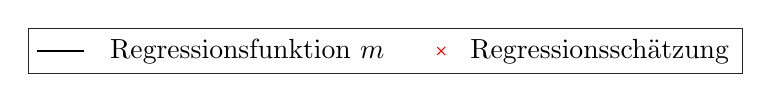
\begin{tikzpicture} 
    \begin{axis}[%
    legend columns=2,
    hide axis,
    xmin=10,
    xmax=50,
    ymin=0,
    ymax=0.4,
    legend style={draw=white!15!black,legend cell align=left,column sep=0.25cm}
    ]
    \addlegendimage{no markers,black}
    \addlegendentry{Regressionsfunktion $m \quad$};
     \addlegendimage{only marks,red,mark=x}
    \addlegendentry{Regressionsschätzung};
    \end{axis}
\end{tikzpicture}}
    \end{subfigure}
     \caption{Approximation der Regressionsfunktion $m(x) = \sin\big(\frac{\pi}{2} \cdot x^2\big)$ durch unseren Neuronale-Netze-Regressionsschätzer mit Parametern $d = 1$, $q = 2$, $R = 10^6$, $a = 3$, $M \in \{2,4,8,9,16\}$ und $N \in \{2,4,8,9,16\}$, wobei wir immer Kombinationen von $M$ und $N$ betrachten, sodass $(M + 1)\cdot(N + 1) \approx 51$ gilt.}
    \label{fig:subfig.a.5}
\end{figure}
\newpage
\section{Vergleich des empirischen $L_2$-Fehlers}

In diesem Abschnitt führen wir nun einen Vergleich des empirischen $L_2$-Fehlers zwischen dem in Abschnitt \ref{Studie} vorgestellten Regressionsschätzer und den Standardschätzern durch, die im Verlauf dieses Abschnitts vorgestellt werden.
Die simulierten Daten, welche wir verwenden werden, sehen wie folgt aus:
Wir wählen $X$ gleichverteilt auf $[-2, 2]^d$, wobei $d \in \{1,2\}$ die Dimension des Inputs ist. Zudem wählen wir $\epsilon$ standardnormalverteilt und unabhängig von $X$ und wir definieren $Y$ durch:
\begin{equation}
    \label{eq:Y}
    Y = m_d(X) + \sigma \cdot \lambda_d \cdot \epsilon,
\end{equation}
wobei $m_d \colon [-2, 2]^d \to \R$ den Regressionsfunktionen
$$ m_1(x) =  \sin\big(0.2 \cdot x^2\big) + \exp(0.5 \cdot x) + x^3$$
und
$$ m_2(x_0, x_1) = \sin\big(\sqrt[2]{x_0^2 + x_1^2}\big)$$
entspricht.
Den Skalierungsfaktor $\lambda_d > 0$ wählen wir als Interquartilsabstand \emph{(IQA)} einer Stichprobe von $m(X)$. Für den Rauschfaktor $\sigma$ gilt $\sigma \in \{0.05, 0.1\}.$ Mit diesen Daten lässt sich nun auch $Y$ darstellen. 

Als Nächstes kommen wir zu den Schätzern, die wir in diesem Abschnitt vergleichen möchten. Für die Wahl der Parameter der jeweiligen Schätzer haben wir uns an \cite{kohler19} orientiert.
Der Schätzer \textit{fc\_neural\_1\_estimate} \todo{Keras erwähnen s.o.} ($m_{n,2}$) ist ein neuronales Netz mit Architektur~$(1,\bk)$, wobei die Anzahl an Neuronen $\bk$ aus der Menge $\{5, 10, 25, 50, 75\}$ stammt. Für das neuronale Netz haben wir die \emph{ReLu} Aktivierungsfunktion $f(x) = \max\{0,x\}$ verwendet. Die Anzahl der Neuronen in der verborgenen Schicht ist so gewählt, dass diese zu einem minimalen empirischen $L_2$-Risiko des Schätzers führt.

Unser nächster Schätzer \textit{nearest\_neighbor\_estimate} ($m_{n,3}$) ist ein Nächste-Nachbar-Schätzer \cite[Kapitel~7.1]{fahrmeir2009regression}, bei dem die Anzahl an nächsten Nachbarn so aus der Menge $\{ 2,3,\dots,9\}$ ausgewählt wird, dass dieser zu einem minimalen empirischen $L_2$-Risiko führt.

Um die Qualität der Schätzung mittels Kennzahlen zu quantifizieren und um diese mit anderen Schätzern zu vergleichen, betrachten wir in Tabelle~\ref{tab:truthTablesm1} und Tabelle~\ref{tab:truthTablesm2} den Interquartilsabstand und den Median des skalierten $L_2$-Fehlers $\epsilon_{L_2}(m_{n,i})$ der einzelnen Schätzer $m_{n,i}$ von einer Stichprobe von Schätzungen. 

Für die Schätzung von $m_1$ setzen wir: $d = 1$, $N = 3$, $q = 2$, $R = 10^6$, $a = 2$, $M = 2$, da diese Wahl der Parameter bereits sehr gute und schnelle Schätzungen liefert. Für die Schätzung von $m_2$ erhalten wir bereits mit: $d = 2$, $N = 2$, $q = 2$, $R = 10^6$, $a = 2$, $M = 2$ sehr gute Schätzungen.

Wir betrachten ein skaliertes Fehlermaß, da wir die zu schätzenden Regressionsfunktionen $m_d$ kennen und der Fehler stark von der Komplexität der zu schätzenden Funktion abhängt. \todo{2 mal gleicher Satzanfang} Dieses skalierte Fehlermaß ist so zu verstehen, dass wir den empirischen $L_2$-Fehler im Verhältnis zum Median des empirischen $L_2$-Fehlers $\bar{\epsilon}_{L_2}$ des simpelsten Schätzers von $m_d$, einer konstanten Funktion, welchen wir als \textit{konstanten Schätzer} bezeichnen, betrachten. Dieses skalierte Fehlermaß ist so zu deuten, dass ein großer Fehler eines Regressionsschätzers im Falle, dass der Fehler des konstanten Schätzers klein ist, auf eine noch schlechtere Leistung hindeutet.

Unser Vorgehen zum Vergleich der drei hier betrachteten Regressionsschätzer gestaltet sich wie folgt:
Da die resultierenden skalierten Fehler noch von der Stichprobe von $(X, Y)$ abhängen und um diese Werte besser vergleichen zu können, führen wir die Fehlerberechnung jeweils $50$ mal durch und geben dann den Median und den Interquartilsabstand für die Schätzung der betrachteten Regressionsschätzer aus.
Um diesen skalierten $L_2$-Fehler in jeder der 50 Iterationen zu bestimmen, gehen wir folgt vor:

Wir teilen die Stichprobe von $X$ in ein Learning-Sample $X_{\text{train}}$ der Größe $n_{\text{train}} = 800$ und in ein Testing-Sample $X_{\text{test}}$ der Größe $n_{\text{test}} = 200$ auf.
Auf dem Learning-Sample werden nun auch die Werte $Y_{\text{train}}$ als Realisierung der Zufallsvariable $Y$ aus Gleichung~\eqref{eq:Y} bestimmt. Jedem einzelnen dieser Schätzer wird nun der Datensatz $(X_{\text{train}},Y_{\text{train}})$ zum Lernen bzw.\@ Festlegen der Parameter gegeben. Wir bestimmen als Erstes den $L_2$-Fehler der einzelnen Schätzer \todo{was ist n?} $m_{n,i}$ mit $i = 1,2,3$ approximativ durch den empirischen $L_2$-Fehler $\epsilon_{L_2}(m_{n,i})$ auf einer unabhängigen Stichprobe $X_{\text{test}}$ der Größe $200.$ Mit dem konstanten Schätzer bestimmen wir nun 25-mal den empirischen $L_2$-Fehler auf einer unabhängigen Stichprobe von $X$ der Größe 200.
Von dieser Stichprobe von Fehlern nehmen wir nun den Median und erhalten so das skalierte Fehlermaß $\epsilon_{L_2}(m_{n,i}) / \bar{\epsilon}_{L_2}.$

%\begin{figure}
%\centering
%%\input{tikzfigure1.tikz}
%\begin{tikzpicture}
%\begin{axis}[x dir=reverse]
%\addplot3 [scatter, only marks]
%  table[x=x, y=y, z=f, col sep=comma] {plotpostpro_sort.csv};
%\end{axis}
%\end{tikzpicture}
%\end{figure}

Wie wir in Tabelle~\ref{tab:truthTablesm1} und Tabelle~\ref{tab:truthTablesm2} anhand des Medians und des IQA des skalierten $L_2$-Fehlers sehen können, übertrifft unserer Neuronale-Netze-Regressionsschätzer in allen Fällen die Leistung der anderen Schätzer. 
\begin{table}
\centering
\begin{tabular}{ |p{5cm}||p{4cm}|p{4cm}|}
 \hline
 & \multicolumn{2}{|c|}{$m_1$}\\
 \hline
 $\sigma$& $5\%$ & $10\%$ \\
 \hline
 $\bar{\epsilon}_{L_2,N}$& $13.4482362$ & $13.3925910$ \\
 \hline
 \textit{Lageparam. (Streuungsmaß) }&  Median (IQA) &  Median (IQA)   \\
 \hline
 new\_neural\_network\_estimate & $\mathbf{2.482\textbf{e-}05 \; (1.612\textbf{e-}05)}$   & $\mathbf{6.908\textbf{e-}05 \; (3.936\textbf{e-}05)}$  \\
 fc\_neural\_1\_estimate & $4.384\text{e-}04 \; (2.14\text{e-}03)$ &   $7.261\text{e-}04 \; (4.57\text{e-}03)$ \\
 nearest\_neighbor\_estimate & $2.9527\text{e-}04 \; (9.312\text{e-}05)$ & $9.0864\text{e-}04 \; (2.895\text{e-}04)$\\
 \hline
\end{tabular}
    \caption{Median und IQR von $50$ skalierten empirischen $L_2$-Fehlers für Schätzungen für $m_1$.}
     \label{tab:truthTablesm1}   
\end{table}
    
    \begin{table}
\centering
\begin{tabular}{ |p{5cm}||p{4cm}|p{4cm}|}
 \hline
 & \multicolumn{2}{|c|}{$m_2$}\\
 \hline
 $\sigma$& $5\%$ & $10\%$ \\
 \hline
 $\bar{\epsilon}_{L_2,N}$& $0.0324$ & $0.0311$ \\
 \hline
 \textit{Lageparam. (Streuungsmaß)}&  Median (IQA) &  Median (IQA)   \\
 \hline
 new\_neural\_network\_estimate & $\mathbf{0.003961 \; (0.000932)}$   & $\mathbf{0.00431 \; (0.000973)}$  \\
 fc\_neural\_1\_estimate & $0.0257 \; (0.3803)$ &   $0.0559 \; (0.52033)$ \\
 nearest\_neighbor\_estimate & $0.01616 \; (0.005906)$ &$0.01763 \; (0.007081)$\\
 \hline
\end{tabular}
    \caption{Median und IQR von $50$ skalierten empirischen $L_2$-Fehlers für Schätzungen $m_2$.}
    \label{tab:truthTablesm2}   
\end{table}
